% !TeX program = xelatex
% 本文档编写于 2022 年 9 月 13 日,使用 TeXLive 2022 编译通过
% 请使用不低于 2021 版的 TeXLive (在苹果系统上可以是 MacTeX) 编译此文档
% 其它编译器不保证编译效果的正确性,不要使用早已过时并且存在许多 bug 的 CTeX 套装

%==============================%
%   清华大学求真书院讲义模板   %
%   清华大学求真书院版权所有   %
%==============================%

% \documentclass[UTF8,oneside,12pt]{book}
\documentclass[oneside,12pt]{book}
                               % UTF8 指定文件编码
                               % oneside 指定书籍为单开页 (防止多余的空白页出现)
\usepackage[a4paper,margin=1in]{geometry}
                               % 设置纸张大小为 A4,页边距为1英寸

\usepackage{amsmath}           % AMS 的主包
% \usepackage{amssymb}           % AMS 符号包,会自动加载 amsfonts
% \usepackage{latexsym}          % 几个额外的特殊符号,包括 \Box
\usepackage{mathrsfs}          % \mathscr 字体样式
% \usepackage{eucal}             % 更改 \mathcal 的字体样式
\usepackage{amsthm}            % AMS 的定理环境
\usepackage{mathtools}         % 一些额外的数学环境功能,包括 \dfrac
\usepackage{stmaryrd}          % 更更多的特殊符号
\usepackage{esint}             % 更多积分符号
\usepackage{extarrows}         % 提供在箭头上下写字的命令
\usepackage{enumerate}         % 带序号列表环境
\usepackage{xcolor}            % 让 latex 支持花里胡哨的颜色的包
\usepackage{graphicx}          % 插入各种类型图片支持
\usepackage{tikz}              % tikz 绘图环境
\usepackage{tikz-3dplot}       % 一个简单的 tikz 3d 绘图宏包
\usepackage{tikz-cd}           % 基于 tikz 的交换图表绘制工具
\usepackage[all,cmtip]{xy}     % 交换图表绘制工具,命令为 \xymatrix
\usepackage{pgfplots}          % 高级绘图包,基于 tikz,包括 2d 和 3d 绘图
\pgfplotsset{compat=newest}    % 设置 pgfplots 兼容性选项,以使用新功能
\usepackage{subcaption}        % 可以交叉引用的图表并排环境
\usepackage[ocgcolorlinks,linkcolor=blue]{hyperref}
                               % 更 fancy (如带颜色,可以点击等等) 的引用
\usepackage{cleveref}          % 更“聪明”的引用,使用此宏包,在引用一个公式/定理等时
                               % 请使用 \cref 而非 \ref
\usepackage[hyperref=true,backend=biber,style=alphabetic,backref=true,url=false]{biblatex}
                               % 使用 biblatex 管理参考文献,后端采用 biber,取代
                               % 古老的 natbib + bibtex,使用方法自行上网查阅
                               % 如果需要用 natbib,请自行注释掉这一行然后正常使用
\usepackage{tcolorbox}         % 绘制彩色文本框的宏包
\tcbuselibrary{most}           % 加载 tcolorbox 的库
% \usepackage{bm}                % 为所有数学字体添加粗体,命令 \bm{abcd}
\usepackage{slashed}           % 在符号上添加反划线,命令 \slashed

%==============================%
%     请在这里添加其它宏包     %
%------------------------------%
% \usepackage{float}           % 我用来防止插图浮动 <- 你不需要它
\usepackage{tensor}            % 张量指标
\usepackage{commath}
\usepackage{physics}           % 提供了方便地打出 d/dx 等符号的命令
\usepackage{engord}            % 英文中的序数    
%==============================%
\usepackage[warnings-off={mathtools-colon,mathtools-overbracket}]{unicode-math}
\usepackage[default]{fontsetup}
%==============================%


%==============================%
%    私货,定义了一些小命令    %
%------------------------------%
\DeclareMathOperator{\sign}{sign}
\DeclareMathOperator{\dom}{dom}
\DeclareMathOperator{\ran}{ran}
\DeclareMathOperator{\ord}{ord}
\DeclareMathOperator{\Span}{span}
\DeclareMathOperator{\img}{Im}
\newcommand{\card}{\texttt{\#}}
\newcommand{\ie}{{\itshape{}\/i.e.}}
\newcommand{\st}{{\itshape{}\/s.t.}}
\newcommand{\eps}{\varepsilon}
\newcommand{\vphi}{\varphi}
\newcommand{\vthe}{\vartheta}
\newcommand{\II}{I\!I}
\renewcommand{\emptyset}{\varnothing}


%==============================%

%==============================%
%         定理环境设置         %
%------------------------------%
\theoremstyle{plain}\newtheorem{theorem}{Theorem}
\theoremstyle{definition}\newtheorem{definition}[theorem]{Definition}
\theoremstyle{plain}\newtheorem{axiom}[theorem]{Axiom}
\theoremstyle{plain}\newtheorem{corollary}[theorem]{Corollary}
\theoremstyle{plain}\newtheorem{lemma}[theorem]{Lemma}
\theoremstyle{plain}\newtheorem{proposition}[theorem]{Proposition}
\theoremstyle{plain}\newtheorem{prop}[theorem]{Proposition}
\theoremstyle{plain}\newtheorem{conjecture}[theorem]{Conjecture}
\theoremstyle{plain}\newtheorem{problem}[theorem]{Problem}
\theoremstyle{plain}\newtheorem{example}[theorem]{Example}
\theoremstyle{plain}\newtheorem{construction}[theorem]{Construction}
\theoremstyle{remark}\newtheorem{notation}[theorem]{Notation}
\theoremstyle{definition}\newtheorem*{question}{Question}
\theoremstyle{definition}\newtheorem*{answer}{Answer}
\theoremstyle{definition}\newtheorem*{goal}{Goal}
\theoremstyle{plain}\newtheorem*{application}{Application}
\theoremstyle{plain}\newtheorem*{exercise}{Exercise}
\theoremstyle{remark}\newtheorem*{remark}{Remark}
\theoremstyle{remark}\newtheorem*{note}{\small{Note}}
\numberwithin{equation}{section}
\numberwithin{theorem}{section}
\numberwithin{figure}{section}
%==============================%

%==============================%
%    定义标题图片和背景图片    %
%------------------------------%
\usepackage{fancyhdr}
\pagestyle{fancy}
\fancypagestyle{plain}{
    \renewcommand{\headrulewidth}{0pt}
    \fancyhead{}
    \chead{
\includegraphics[width=0.4\linewidth]{picture/qiuzhen.png}} 
}
\renewcommand{\headrulewidth}{0pt}
\addtolength{\headheight}{0.030\paperheight}
\addtolength{\topmargin}{-0.030\paperheight}
\fancyhead{}
\chead{
\includegraphics[width=0.4\linewidth]{picture/qiuzhen.png}} 
%------------------------------%
% \usepackage{eso-pic}
\DeclareHookRule{shipout/background}{title/opac}{before}{pgfrcs}
\AddToHook{shipout/background}[title/opac]{
    \begin{tikzpicture}[remember picture,overlay]
        \centering
        \node [opacity=0.1] at (current page.center) {
            
\includegraphics[height=0.2\paperheight]{picture/redqiuzhen.png}
        };
    \end{tikzpicture}
}
%==============================%

%==============================%
%  添加参考文献库 (.bib 文件)  %
%  例 \addbibresource{XX.bib}  %
%------------------------------%

\addbibresource{}

%==============================%

%==============================%
% 定义封面样式,请将 XX 替换为 %
% 具体的课程名和人名           %
%------------------------------%
\title{
    \huge{Differential Geometry~~Lecture Notes}
    \vspace{0.4\paperheight}
}
\author{
    \Large{Instructor: Zhang Yingying}\\
    \Large{Notes Taker: Xue Haotian, Yan Guangxi}
    \vspace{0.1\paperheight}
}
\date{
    \Large{Qiuzhen College, Tsinghua University}\\
    \Large{2022 Fall}
}                                         
%==============================%

\begin{document}
\maketitle
\frontmatter
\tableofcontents
\newpage

%==============================%
%           正文内容           %
%------------------------------%

\mainmatter{}

\chapter*{\centering Preface}
\addcontentsline{toc}{chapter}{Preface}
\setlength{\headheight}{33.24858pt}
\section*{Textbook Reference}
\begin{enumerate}[(1)]
    \item Do Carmo: Differential Geometry of Curves and Surfaces.
    \item Sebasti\'an Montiel, Antorio Ros: Curves and Surfaces.
    \item \textit{Chinese Title, add later}
\end{enumerate}
\section*{Course Introduction}
The Goal of this course is to study the ``differential geometry of curves and surfaces''.

\noindent
$\bullet$ \textbf{Geometry}: How is a geometric object curved / How to measure the curvedness of a geometric object? 
\begin{example}
     In the illustration below, (1) differs by ``topology''. In (2), they are topologically the same, while the lower curve is ``more curved'' than the upper curve.
\end{example}

\begin{center}
    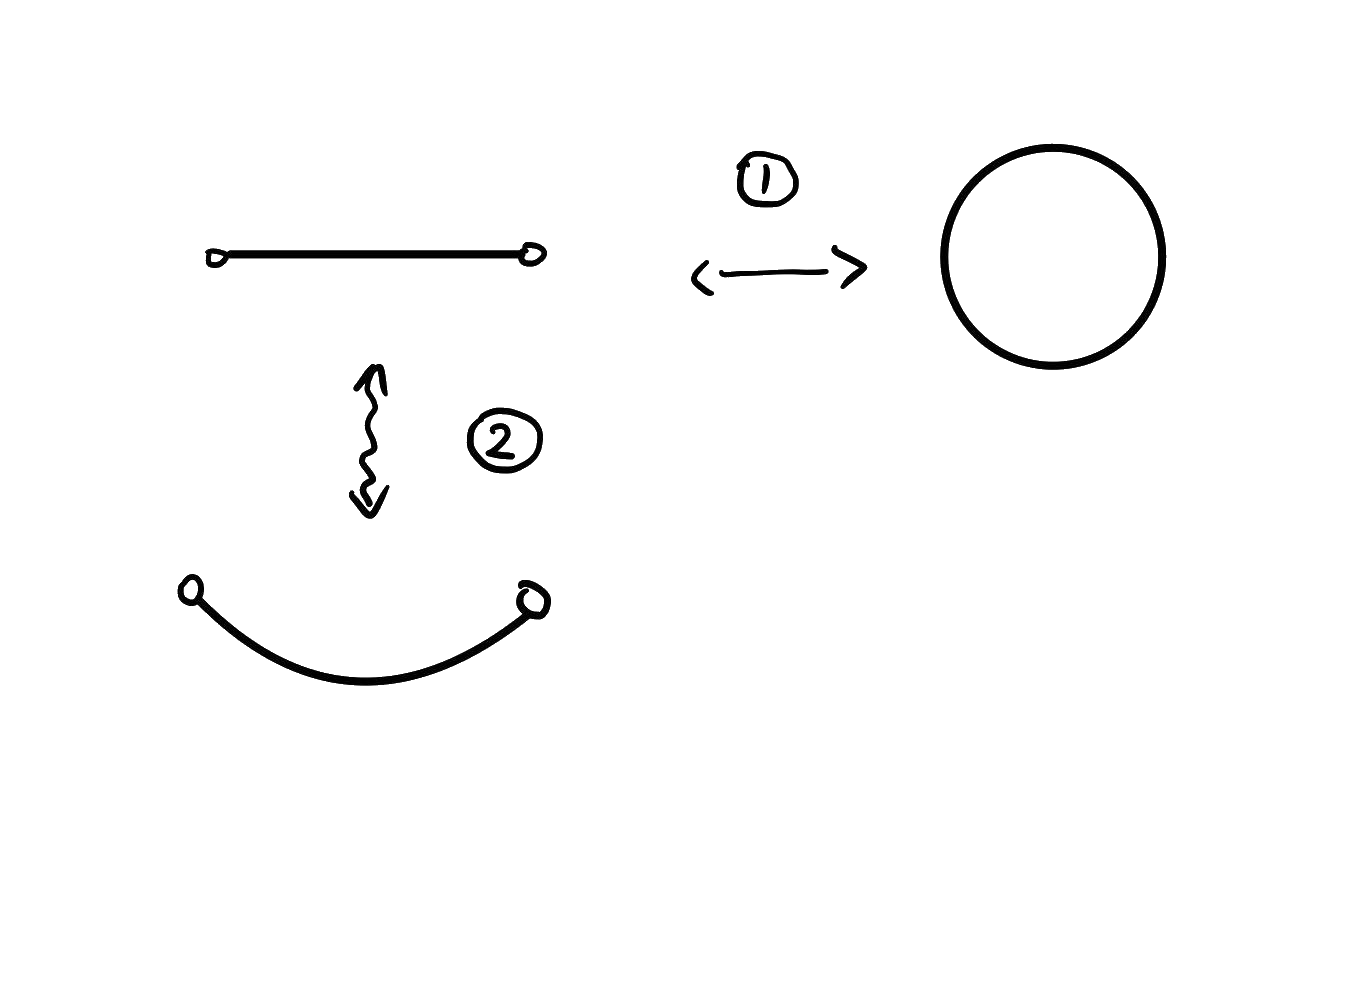
\includegraphics[scale=0.3]{picture/preface/preface_example1.png}
\end{center}

\begin{example}
    (3) differs by ``topology'', but in (4) $\mathbb{S}^2(1)$ is more curve than $\mathbb{S}^2(2)$, even topologically they are the same.(either homeomorphically or diffeomorhically).
\end{example}

\begin{center}
    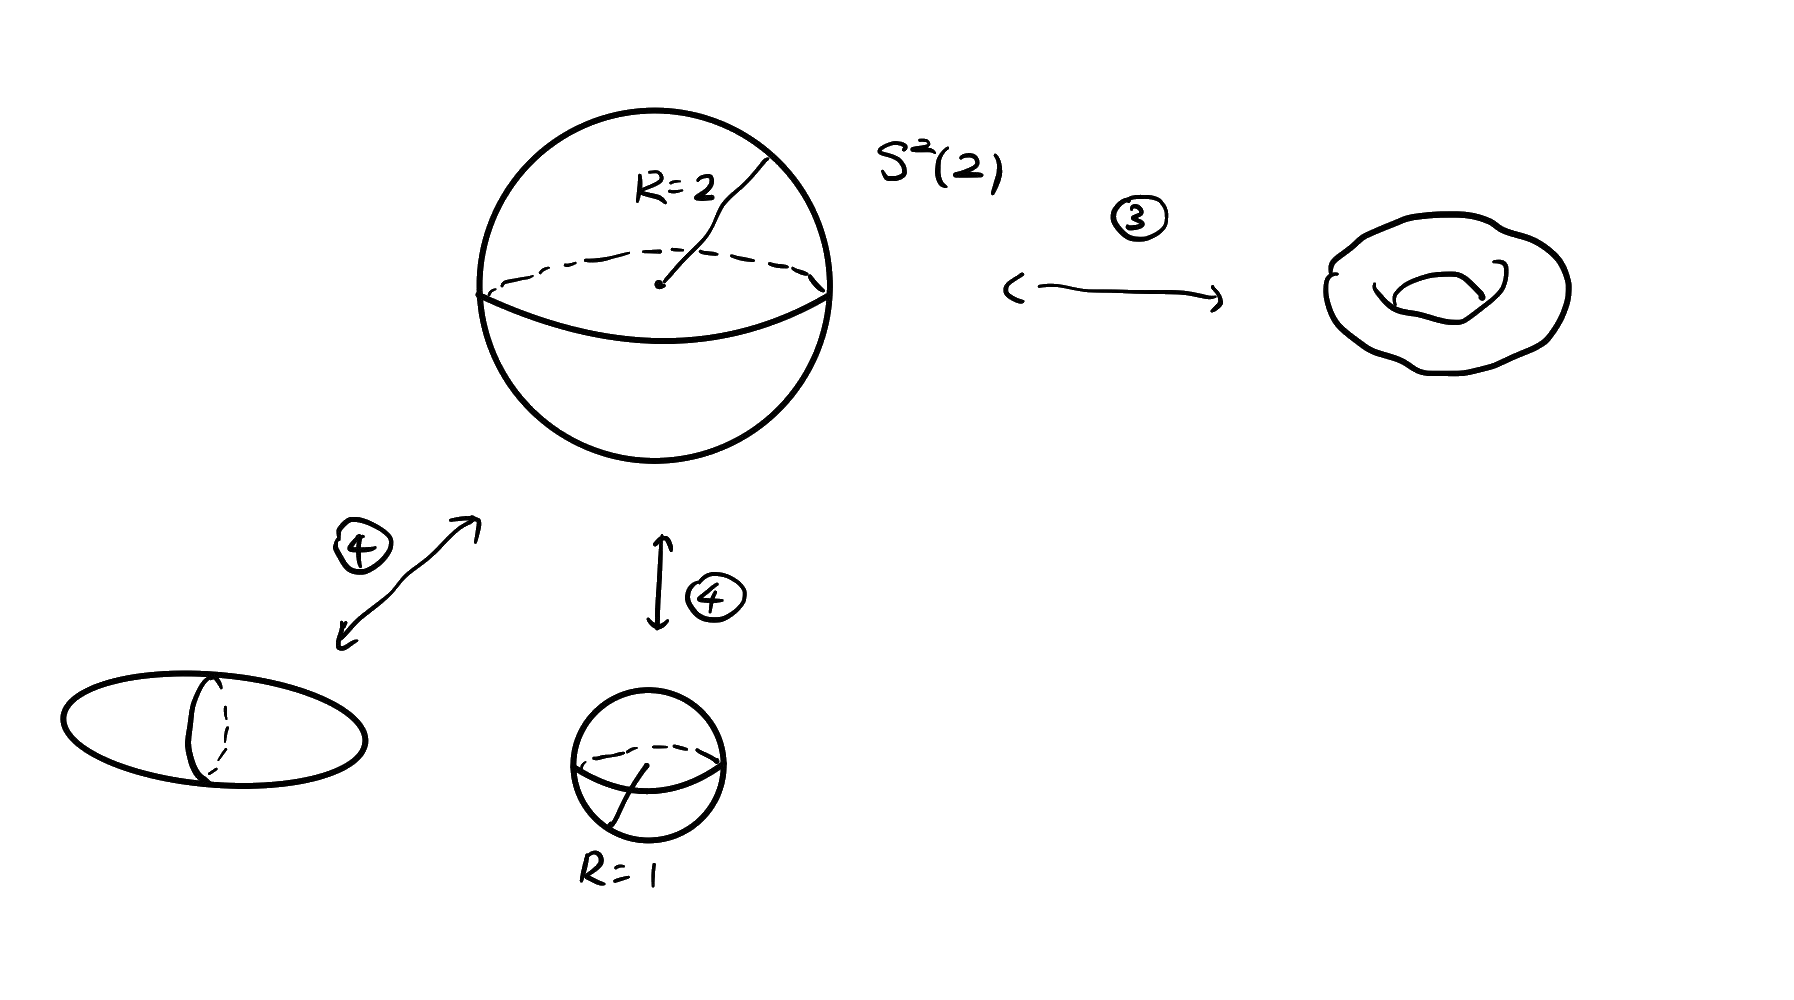
\includegraphics[scale=0.2]{picture/preface/preface_example2.png}
\end{center}

The ``Curved property'' also affects geometric quantities, like length, area, volume, angle between the curves, etc.

\textbf{Local Geometry}: How does a ``curved '' space look like in a neighborhood of a point?
 
\textbf{Global Geometry}: If we know how a ``curved space'' is look like at each point, can we observe how such space looks like globally? This is usually related to topological problems.

$\bullet$ \textbf{Differential}: In this course, by ``smoothness'' we mean the geometric objects we'll study are ``nice'' enough so we can apply ``calculus'' tools to study them.

\textbf{Main tool}: Calculus! We'll see how powerful calculus is in this course, especially, like the maximal principle, integration by parts(stoke's theorem), Taylor's expansion, implicit function theory, etc.

\begin{center}
    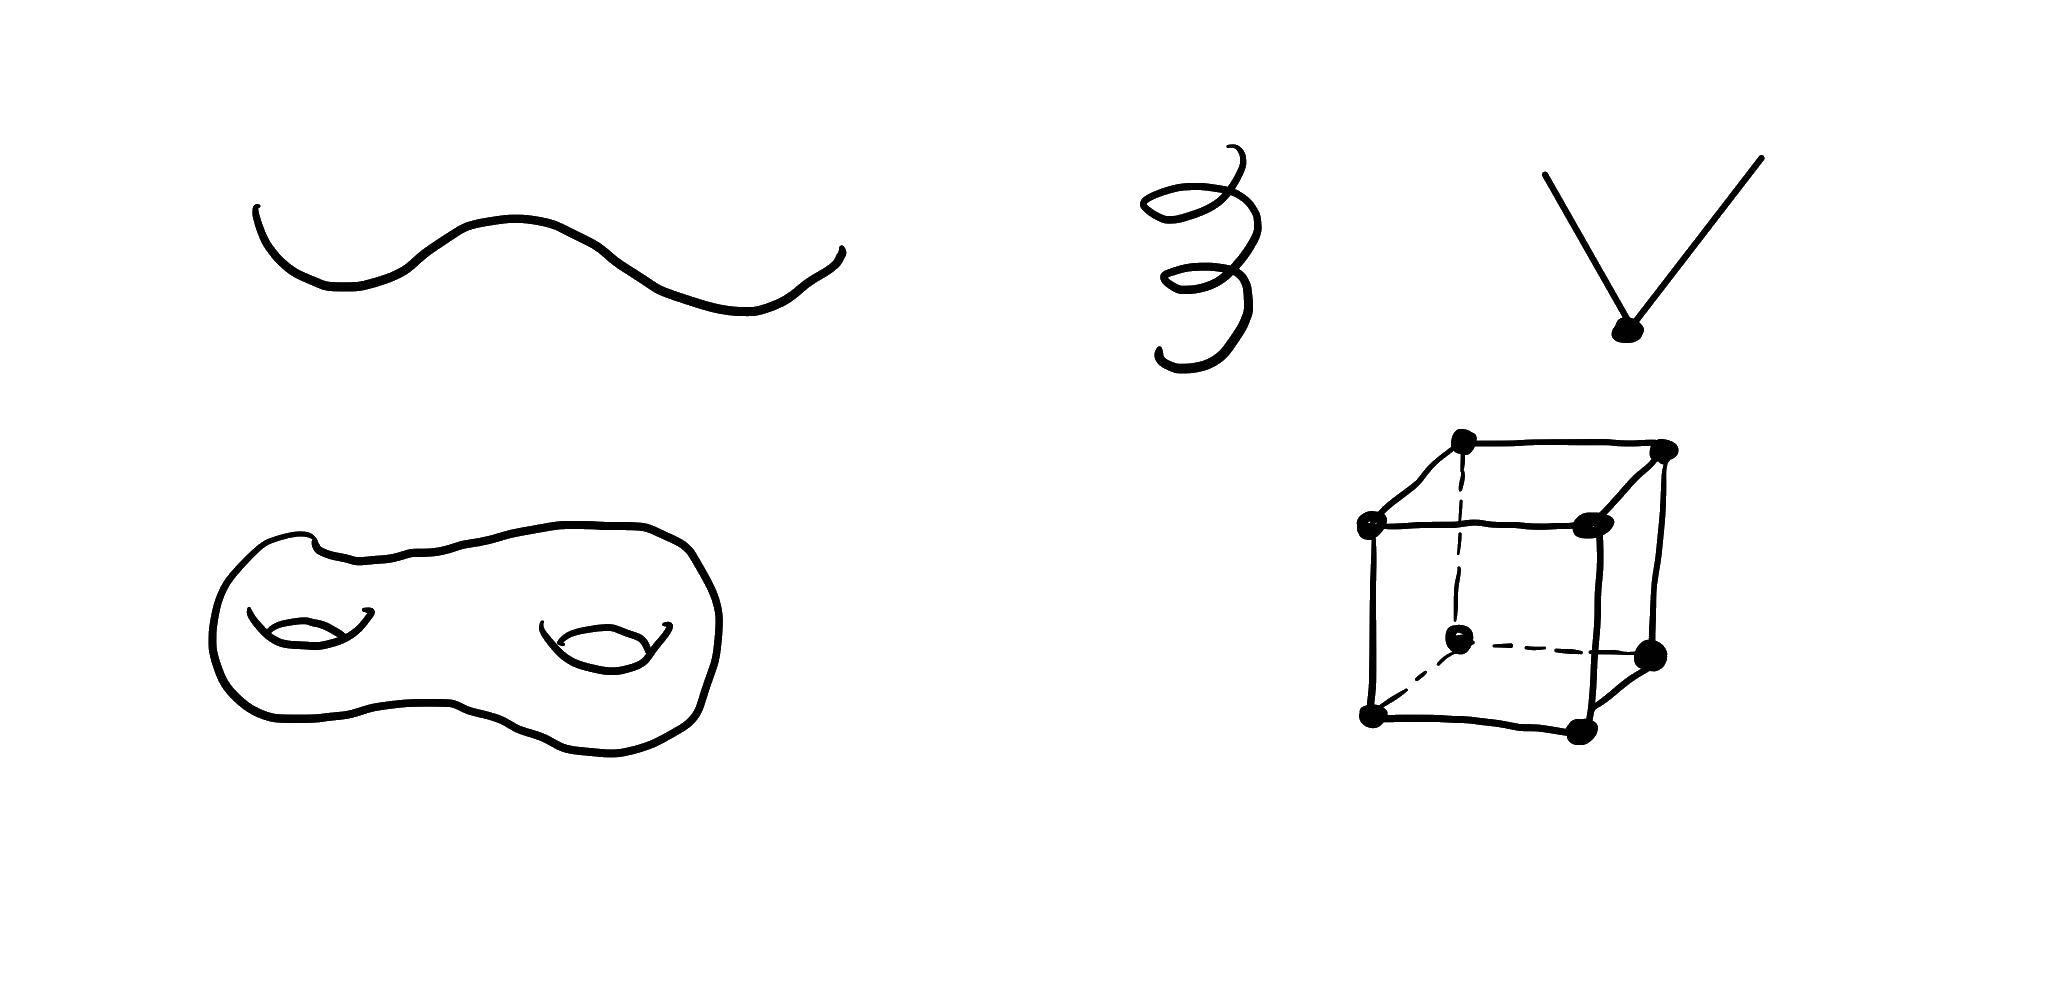
\includegraphics[scale=0.2]{picture/preface/preface_example3.png}
\end{center}

Queastion: How to tell the ``smoothness''?(Need to find good parametrization)Finding a good ``gauge''(that is ``coordinate'') to work with is also an important question in geometry.

$\bullet$Curves: 1-d geometric object.

Surfaces: 2-d geometric object.
\begin{remark}
    In this course, we only focus on curves and surfaces in $\mathbb{R}^3$.However, as a training on preparing for later geometry course, I suggest you also try to think about the ambiant space is $\mathbb{S}^3$ or $\mathbb{H}^3$.

\end{remark}
$\bullet$\textbf{Intrinsic geometry}: Study the geometric object without considering the ambient space. This begins from the Gauss's elegant theorem and was developed by Riemann.
\begin{example}
    Consider the unit sphere $\mathbb{S}^2$

    Extrinsic geometry: view it as $x^2+y^2+z^2=1$ in $\mathbb{R}^3$.

    Intrinsic geometry: $(\theta,\varphi)$ or $(\varphi,\theta)$ are ``essential'' coordinates on $\mathbb{S}^2$. \[
        \dd s^2=\dd \varphi^2+(\sin\varphi)^2 \dd\theta^2
    \]

    (Caution: $(\theta,\varphi)$ is outer normal, while $(\varphi,\theta)$ is inner normal.)
\end{example}
$\bullet$ Useful / Common techniques:
\begin{enumerate}[1)]
    \item Comparison: compare the studied geometric object with ``model space''. It's very important to study examples in geometry. As a suggestion you are expected to spend time to play with $\mathbb{S}^2$.For example: How is $\mathbb{S}^2$ curved? What's the shortest line in $\mathbb{S}^2$? How many symmetries are there on $\mathbb{S}^2$? Can you add ``extra structure'' on$\mathbb{S}^2$ to make it a complex object? Is this ``extra structure'' ``rigid''?What/s the ``moment map'' on $\mathbb{S}^2$? Does there exist a ``holomorphic'' map from $\mathbb{S}^2$ to a torus, or a surface of arbitrary genus? 
 
    If we consider an ``Energy minimizing map'' from $\mathbb{S}^2$ to $\mathbb{S}^2$, what can we say about such map?(It is  holomorphic/antiholomorphic.)
 
    After you have learned Riemann Geometry, you'll see an energy minimizing map from $\mathbb{S}^2$ to a Riemannian manifold must be an angle-preserving map(conformal map).
 
    What kinds of 2-d geometric space could be $\mathbb{S}^2$ ?(this is a global geometry problem.)(\ie\ what kinds of geometric conditions can characterize $\mathbb{S}^2$ ?)
    \item To study higher dimensional objects,it's also important to understand lower dimensional objects, and it's also important to understand lower dimensional objects contained in the studied objects.
    \item Study ``functions'' (more generally sections, including functions, vector fields, differential forms, etc.) on a given geometric object.
\end{enumerate}
\begin{example}
    On a closed surface ( $\mathbb{S}^2$,$\mathbb{T}^2$,$\Sigma_g$)(compact without boundary) there is no non-constant harmonic function.(i.e. $\Delta u=0$)(Analysis will get involved.)
\end{example}
We usually care about those functions related to geometry, such as distance functions, curvature-related functions, etc.
\begin{example}[More trivial than the last one]
    Consider $f''(x)=0$, what can you say of the solution of it when $x$ lies on a line and when $x$ lies on a circle?
\end{example}


\chapter{Differential Geometry of Curves}
\section{Linear algebra convention and its geometric explanation}
\begin{itemize}
    \item We use ``ROW VECTOR'' in this course, \ie\
    \[v\in \mathbb{R}^n, v=(v_1,v_2,\cdots,v_n)\]
    \item let $e_1=(1,0,\cdots,0),\cdots,e_n=(0,\cdots,1)$ be the standard basis, then 
    \[v=\sum_{i=1}^nv^i e_i=
    \begin{bmatrix}
        v^1& v^2& \cdots & v^n
    \end{bmatrix}
    \begin{bmatrix}
        e_1\\
        e_2\\
        \vdots\\
        e_n
    \end{bmatrix}
    \]
    \item $\varphi\colon \mathbb{R}^n\to \mathbb{R}^n$ (non-degenerate) linear map
    \[v\mapsto \varphi(v)=v\cdot A.\]
    This corresponds to the right action of $GL(n,\mathbb{R})$ on $\mathbb{R}^n$.
    \[\Rightarrow \varphi(e_i)=e_j \cdot A=\sum_{i=1}^n A\indices{_j^i}e_i\text{ (taking the j-th row of }A\text{)}\]
    
    \[A\indices{_j^i}\begin{cases}
        \text{upper index: column index}\\
        \text{lower index: row index}
    \end{cases}\]
    \[\Rightarrow \varphi\begin{bmatrix}
        e_1\\
        e_2\\
        \vdots\\
        e_n
    \end{bmatrix}=\begin{bmatrix}
       \varphi( e_1)\\
        \varphi (e_2)\\
        \vdots\\
        \varphi(e_n)
    \end{bmatrix}=\begin{bmatrix}
        e_1\cdot A\\
        e_2\cdot A\\
        \vdots\\
        e_n\cdot A
    \end{bmatrix}=
    A \begin{bmatrix}
        e_1\\
        e_2\\
        \vdots\\
        e_n
    \end{bmatrix}\]
\end{itemize}
\begin{remark}[Important!]
    In row vector convention, a non-degenerate linear map corresponds to the right action of $GL(n,\mathbb{R})$ on $\mathbb{R}^n$. But this induces left action of $GL(n,\mathbb{R})$ on the orthonormal basis (frame) $\{e_1,e_2,\ldots,e_n\}$. This phenomenon provides an important example in differential geometry, which will be explained later in the theory of principle bundle.(\ie\ let $G$ be a lie group, $G\curvearrowright M$ being a right action, where $M$ is a differentiable manifold, then this right action induces a left action of $G$ on the frame bundle of $M$.)
 \end{remark}
 
 
 Let $\{\tilde{e}_1,\ldots,\tilde{e}_n\}$ be another basis of $\mathbb{R}^n$. Let $f$ be the corresponding linear map, \ie\
 \[f\begin{bmatrix}
    e_1\\
    e_2\\
    \vdots\\
    e_n
\end{bmatrix}=\begin{bmatrix}
    \tilde{e}_1\\
    \tilde{e}_2\\
    \vdots\\
    \tilde{e}_n
\end{bmatrix}=B \cdot \begin{bmatrix}
    e_1\\
    e_2\\
    \vdots\\
    e_n
\end{bmatrix}\]
\[\Rightarrow \tilde{e}_k=\sum_{j=1}^n B\indices{_k^j}e_j\]
We compare the matrix of $\varphi$ in terms of $\left\{\tilde{e}_1 \cdots \tilde{e}_n\right\}$
\[
    \varphi\left[\begin{array}{c}\tilde{e}_1 \\ \vdots \\ \tilde{e}_n\end{array}\right]=\varphi\left[B\left[\begin{array}{c}\tilde{e}_1 \\ \vdots \\ e_n\end{array}\right]\right]=B \cdot \varphi\left[\begin{array}{c}e_1 \\ \vdots \\ e_n\end{array}\right]\text{(linearity of }\varphi\text{)}
\]
\[
    =B A\left[\begin{array}{c}
    e_1 \\
    \vdots \\
    e_n
    \end{array}\right]=B A B^{-1}\left[\begin{array}{c}
    \tilde{e}_1 \\
    \vdots \\
    e_n
    \end{array}\right]
\]
Note in this case.
\[
(\varphi \circ f)\left[\begin{array}{c}
e_1 \\
\vdots \\
e_n
\end{array}\right]=B A\left[\begin{array}{c}
e_1 \\
\vdots \\
e_n
\end{array}\right]
\]
In terms of entries,
\begin{align*}
    \varphi(\tilde{e}_k) &=\varphi(\sum_{j=1}^n B\indices{_k^j} e_j)=\sum_{j=1}^n B\indices{_k^j} \varphi(e_j) \quad \text { (linearity) } \\
    &=\sum_{i, j=1}^n B\indices{_k^j} A\indices{_j^i} e_i=\sum_{i,j,p=1}^n B\indices{_k^j} A\indices{_j^i}(B^{-1})\indices{_i^p} \widetilde{e}_p
\end{align*}
\begin{remark}
    This computation tells that the row vector convention yields to the fact that $GL(n,\mathbb{R})$ acting on itself from the right when we consider the action of $GL(n, \mathbb{R})$ on $\mathbb{R}^n$.
    In modern Geometry, it's more common to use column vector as convention. This row vector convention was adopted by S.S. Chern and also Do Cormo's book.
\end{remark}
\section{Parametrized Curves}
\begin{definition}
    Let $I=(a,b)$, if $\alpha\colon I\to \mathbb{R}^3$ is a $C^\infty$ map,
    \[t \mapsto (x(t),y(t),z(t))\]
    then $\alpha(t)$ is a parametrized differentiable curve in $\mathbb{R}^3$. The image of $\alpha$ is called the trace of the curve. 
\end{definition}
\begin{remark}
    \hfill
    \begin{enumerate}[1)]
        \item $a,b$ could be finite number or infinity.
        \item Same curve may have different parametrizations.
        \item The parametrization automatically gives the direction of the motion on the curve.
        \item ``Differentiable'' just means $\alpha(t)$ is a $C^\infty$ \textbf{map}, it does not say the (trace of) curve can not have singularities.
    \end{enumerate}
\end{remark}
\begin{example}
    \hfill
    \begin{enumerate}[(1)]
        \item $\alpha(t)=(t,|t|)$ is not a differentiable curve.
        \begin{center}
            \begin{tikzpicture}
                \draw[domain=-2:0,smooth,variable=\t,black]
                plot (\t,{-\t});
                \draw[domain=0:2,smooth,variable=\t,black]
                plot (\t,\t);    
                \draw (0,0) node{$\bullet$};
                \draw[->] (-2,0) -- (2,0) node[right] {$x$};
                \draw[->] (0,-0.5) -- (0,2.5) node[above] {$y$};
            \end{tikzpicture}
        \end{center}
        \item $\alpha=(t^3,t^2)$ is a differentiable curve. It can be also given by a equation $y^3=x^2$, which is a cuspidal cubic curve.
        \begin{center}
            \begin{tikzpicture}
                \draw[domain=-1.5:1.5,smooth,variable=\t,black]
                plot ({\t^3},{\t*\t});
                \draw (0,0) node{$\bullet$};
                \draw[->] (-2,0) -- (2,0) node[right] {$x$};
                \draw[->] (0,-0.5) -- (0,2.5) node[above] {$y$};
            \end{tikzpicture}
        \end{center}
        \item $\alpha(t)=(t^2-1,t^3-t)$. This parametrization appers in the ``blow-up'' process of $y^2=x^3+x^2$. Here ``blow-up'' is introducing tangents to seperate points.
        \begin{center}
            \begin{tikzpicture}
                \draw[domain=-1.5:1.5,smooth,variable=\t,black]
                plot ({\t*\t-1},{\t^3-\t});
                \draw (0,0) node{$\bullet$};
                \draw[->] (-2,0) -- (2,0) node[right] {$x$};
                \draw[->] (0,-2.5) -- (0,2.5) node[above] {$y$};
            \end{tikzpicture}
        \end{center}
    \end{enumerate}
\end{example}
\begin{remark}
    (2) and (3) above may be the first examples you'll see in an algebraic geometry course.
\end{remark}
\noindent
\textbf{Question}: At the origin, what can you obsefve on (2) and (3)?

\noindent
\textbf{Answer}:
    (2) $\alpha'(0)=0$.
    (3) $\alpha$ is not one to one, but $\alpha'(0)\neq 0$.

\noindent 
\textbf{Question}: Define a differentiable curve in $\mathbb{R}^3$ and $\mathbb{S}^n$.
\begin{remark}
    Among above differentiable parametrizations, (2) and (3) are differentiable curves. However, if we take $\beta(t)=(t,t^{\frac{2}{3}})$, this also parametrizes (2), but it's not a differentiable curve!
\end{remark}
\begin{definition}
    Let $\alpha(t)\colon I\to \mathbb{R}^3$ be a parametrized differentiable curve, then at $t_0\in I$.
    \[ \alpha'(t_0)=(x'(t_0),y'(t_0),z'(t_0))\]
    is the velocity of $\alpha(t)$ at $t_0$.
    \begin{enumerate}[(1)]
        \item If $\alpha'(t_0)\neq 0$, we call $\alpha(t_0)$ a regular point.
        \item If $\alpha'(t_0) = 0$, we call $\alpha(t_0)$ a singular point.
        \item If for all $t\in I$, $\alpha'(t)\neq 0$, we call $\alpha(t)$ a regular curve.
    \end{enumerate}
\end{definition}
\noindent
\textbf{Question}: What can you say about $C^\infty$ parametrization for a regular curve?
\begin{quotation}
Regular curve $\Longleftrightarrow $ at each point, there is a unique tangent line.
\end{quotation}
\begin{example}
$\alpha(t)=(t^3,t^2)$ is not a regular curve. (Since $\alpha'(0)=0$)
\begin{center}
    \begin{tikzpicture}
        \draw[domain=-1.5:1.5,smooth,variable=\t,black]
        plot ({\t^3},{\t*\t});
        \draw (0,0) node{$\bullet$};
        \draw[->] (-2,0) -- (2,0) node[right] {$x$};
        \draw[->] (0,-0.5) -- (0,2.5) node[above] {$y$};
    \end{tikzpicture}
\end{center}
\end{example}
\begin{example}
$\alpha(t)=(t^2-1,t^3,t)$ is a regular curve.
\begin{center}
    \begin{tikzpicture}
        \draw[domain=-1.5:1.5,smooth,variable=\t,black]
        plot ({\t*\t-1},{\t^3-\t});
        \draw (0,0) node{$\bullet$};
        \draw[->] (-2,0) -- (2,0) node[right] {$x$};
        \draw[->] (0,-2.5) -- (0,2.5) node[above] {$y$};
    \end{tikzpicture}
\end{center}
\end{example}
\begin{definition}
Let $\alpha(t)$ be a regular curve, then the tangent line at $t_0$ is \[l(t)=\alpha(t_0)+\alpha'(t_0)(t-t_0))\]
\begin{center}
    \begin{tikzpicture}[scale=1.25]
    \draw (0, -1) .. controls (1.5, 2) and (2, -3) .. (4,1.5)    % 绘制曲线
        node[
            pos = 0.6,    % 设置切点在曲线上的位置
            sloped,    % 设置node按曲线斜率旋转
            anchor = south west
            ] (N) {};
         

    \draw[blue]($(N.south west)!0.6cm!180:(N.south east)$) -- ($(N.south west)!0.6cm!(N.south east)$);
    \draw (0, -1) .. controls (1.5, 2) and (2, -3) .. (4,1.5)
        node[
        pos = 0.2,    % 设置切点在曲线上的位置
        sloped,    % 设置node按曲线斜率旋转
        anchor = south west
        ] (M) {}; 
    \draw[cyan]($(M.south west)!0.6cm!180:(M.south east)$) -- ($(M.south west)!0.6cm!(M.south east)$);
    \draw (0, -1) .. controls (1.5, 2) and (2, -3) .. (4,1.5)
        node[
        pos = 0.9,    % 设置切点在曲线上的位置
        sloped,    % 设置node按曲线斜率旋转
        anchor = south west
        ] (M) {}; 
    \draw($(M.south west)!1cm!180:(M.south east)$) -- ($(M.south west)!1cm!(M.south east)$);
    \end{tikzpicture}
\end{center}
\end{definition}
\begin{definition}
    Let $\alpha(t)$ be a regular curve, the arc-length of $\alpha(t)$ is 
    \[s(t)=\int_{t_0}^t \left|\alpha'(t)\right|\dd t.\]
    Then $s'(t)=\left|\alpha'(t)\right|$
\end{definition}
\textbf{Question} What's $\left|\alpha'(t)\right|$?

 
$\alpha(t)\colon I\to \mathbb{R}^3$ is a curve in $\mathbb{R}^3$. Here on $\mathbb{R}^3$, as the Euclidean space, we always assume the standard Euclidean inner product on it, \ie\ $\forall u=(u_1,u_2,u_3),v=(v_1,v_2,v_3)$
\[\langle u,v\rangle=u_1 v_1+u_2 v_2+ u_3 v_3=\sum_{i,j=1}^3\delta_{ij}u_i v_j\]
Let $\alpha(t)=(x(t),y(t),z(t)),\alpha'(t)=(x'(t),y'(t),z'(t))$, then $\left|\alpha'(t)\right|=\sqrt{\langle\alpha'(t),\alpha'(t)\rangle}$
\begin{exercise}
    Review vector Calculations, such as dot product, cross product and their properties, especially geometric meanie of these calculation, such as length, area, volume, angle, orientation, etc.
\end{exercise}
\noindent
\textbf{Question}: Can you define the arclength of a regular curve in $\mathbb{R}^n$? How about on $\mathbb{S}^n$? \\
$\bullet$ Arclength parameter(an intrinsic parametrization of a curve)
\begin{example}
On a straight line, x=t describes the distance of the point away from the origin.
\begin{center}
    \begin{tikzpicture}
        \draw[->] (-2,0) -- (2,0) node[right] {};
        \draw (-1,0.05) node{$\bullet$};
        \draw (0.2,0.2) node{$t$};
        \draw[->,blue] (-1,0.1)--(0,0.1) node[right] {};
    \end{tikzpicture}
\end{center}
\end{example}
On a general curve, we also want ``some'' parameter, which describes the arclength of point away from the initial point. This can happen iff $|\alpha'(t)|=1$,\ie\ a point on the curve moves in a unit speed.
\[\Rightarrow s(t)=\int_0^t \dd t=t.\]
\textbf{Question}: For a given regular curve $\alpha(t)\colon I\to \mathbb{R}^3$, how to find such parameter?

\noindent 
\textbf{Answer}: $s(t)=\int_{t_0}^t \left|\alpha'(t)\right|\dd t$ is a function in t, and $s'(t)=\left|\alpha'(t)\right|\neq 0$(because the curve is regular). By the implicit function theorem, there is a function 
\[
    t=t(s),t'(s)=\frac{1}{\left|\alpha'(t)\right|}.
\]
This implies that 
\[
    \alpha(t)=\alpha(t(s))=(x(t(s)),y(t(s)),z(t(s)))
\]
\[
    \left|\alpha'(s)\right|=\left|\alpha'(t)t'(s)\right|=\left|\alpha'(t)\right|\left|t'(s)\right|=1
\]

\boxed{\textbf{Convention}} In this course, we only consider differentiable regular curves, which are parametrized by the arclength (for convenience).
\begin{remark}
    In this course, we only consider the curve without self-intersecting points, i.e curves ``embedded into'' $\mathbb{R}^3$. Here ``embedded'' means $d\alpha$ is a linear isomorphism and $\alpha$ is homeomorphic to its image.
\end{remark}

\section{Local theory of a regular space curve}

\begin{goal}
    Describe a space curve by using geometric quantities.
\end{goal}

\begin{ques}
    How to make a space curve? 
\end{ques}
Starting with a straight line, we can bend it and twist it in a given way to
produce a space curve.
\begin{itemize}
    \item Bending the line \(\longrightarrow\) ``curvature''.
    \item Twisting \(\longrightarrow\) ``torsion''.
    \item Their relations are contained in Frenet formula.
    \item Conversely, fundamental theorem of the local theory of curves
        tells, once we're given two function, \(\kappa(s),\tau(s)\), we can
        describe a unique curve in \(\mathbb{R}^3\) up to a rigid motion,
        \st\ \(\kappa(s)\) is its curvature and \(\tau(s)\) is its torsion.
\end{itemize}

\noindent\underline{\bf Recall:} In Calculus, if \(y=f(x)\) represents a curve, then
\(f''(x)\) tells the convexity of the curve. It measures how fast the velocity
changes. It's also related to how straight line is bent.


Let \(\alpha\colon I\to \mathbb{R}^2\) be a regular plane curve, parametrized by
arc length, \ie\ \(|\alpha'(s)|=1\). Then \(\left<\alpha'(s),\alpha''(s)\right> =0\),
and hence \(\alpha''(s)\perp\alpha'(s)\). For a plane curve, we take normal of the
curve to be counterclockwise \(90^\circ\) rotation of the tangent vector.

% Figure fig:w2-plane-curve-eg here

Let \(N\) be the unit normal vector along \(\alpha(s)\), we have \[
    \left<\alpha''(s),N(s)\right> =\pm|\alpha''(s)|
.\] 
\begin{defn}
    The curvature of a plane curve \(\alpha(s)\) is defined as \[
        \kappa(s)=\left<\alpha''(s),N(s)\right>
    .\] 
\end{defn}
\begin{defn}
    Further we denote \(T\) be the unit tangent vector, then the Frenet equation
    of \(\alpha(s)\) is \[
        \begin{cases}
            T'=\kappa N \\
            N'=-\kappa T
        \end{cases}
    .\] Note that \[
        \left<T',N\right> =\kappa\implies \left<T,N'\right> =-\kappa
    .\] 
\end{defn}

\begin{itemize}
    \item \(\kappa>0\implies \) the point on the curve moves counterclockwise
        direction or say ``to its left''.
    \item \(\kappa<0\implies \) the point on the curve moves clockwise direction
        or say ``to its right''.
\end{itemize}

\begin{ques}
    For the curve in \cref{fig:w2-plane-curve-eg}, can you tell where \(\kappa>0\)
    and where \(\kappa<0\) without doing calculation?
\end{ques}

\begin{remark}
    The sign of the curvature of the plane curve is caused by the direction
    convention of the unit normal vector. This could change according to the
    orientation of a curve.
\end{remark}

Next, we take a look at the geometric meaning of \(|\alpha''(s)|\) at some point
\(\alpha(s_0)\). By definition: \[
    |\alpha''(s_0)|=\lim_{h \to 0} \left|\frac{\alpha'(s_0+h)-\alpha'(s_0)}{h}\right|
.\] 
% May be figure here
We have
\begin{align*}
    |\alpha'(s_0+h)-\alpha'(s_0)|
    &= \left(|\alpha'(s_0+h)|^2+|\alpha'(s_0)|^2-2\left<\alpha'(s_0+h),
    \alpha'(s_0)\right> \right)^{\frac{1}{2}} \\
    &= (2-2\cos\theta_h)^{\frac{1}{2}} \\
    &= (2-2(1-\frac{1}{2}\theta_h^2)+\tilde{o}(\theta_h)^4)^{\frac{1}{2}} \\
    &= (\theta_h^2+\tilde{o}(\theta_h)^4)^{\frac{1}{2}}
.\end{align*}
Hence \[
    |\alpha''(s_0)|=\lim_{h \to 0} \left|\frac{\alpha'(s_0+h)-\alpha'(s_0)}{h}\right|
    =\lim_{h \to 0} \left|\frac{\theta_h}{h}\right|=|\theta'(s_0)|
.\] \ie\ \(|\alpha''(s)|\) measures the changing rate of angle of tangents.

\section{Global theory of plane curves}

The global theory is related to ``topology'' of the geometric objects.
For 1-dimensional geometry, \ie\ curves, it's always oriented. And the simplest distinction in topology
is ``open'' and ``closed''.

\begin{definition}[Closed curves]
    \begin{itemize}\hfill
        \item We say
              \(\alpha\colon I=[a,b]\to \mathbb{R}
              ^3\)
              (or \(\mathbb{R}^2\))
              is a closed regular curve, if
              \(\alpha(a)=\alpha(b)\)
              and
              \(\alpha^{(k)}
              (a)=\alpha^{(k)}(b)\)
              (in another word,
              \(\alpha\colon \mathbb{S}^1\to \mathbb{R}^3\)
              is a differentiable curve).
        \item Furthermore, if
              \(\alpha\)
              has no
              self-intersection point other than
              $\alpha(a)=\alpha(b)$,
              then we call $\alpha(s)$ to be a simple closed curve.
    \end{itemize}
\end{definition}
\begin{center}
    \begin{tikzpicture}
        \draw plot [smooth cycle] coordinates {(0,0) (1,1) (3,1) (1,0) (2,-1)};
    \end{tikzpicture}
\end{center}

\subsection{Isoperimetric inequality}
This is one of the oldest and most famous problem in geometry. It's still attracting mathematicians to investigate such problem in various geometric formulations nowadays.
\begin{question}
    Given a closed plane curve \(C\) with. Let \(D\) be the
    region bounded by \(C\). When does the region have the
    maximal area, if \(C\) is among all the curves with
    fixed length?
\end{question}
\begin{answer}
    \(C\) must be a circle when the maximal area is
    achieved.
\end{answer}
\begin{remark}
    Even though we'll only handle smooth, simple closed
    curves in the following discussion, in general we
    don't have to assume the curve to be simple:
    {\ooalign{$\bigcirc $\cr $\ \ \,\bigcirc $}}
    has less area than $\bigcirc $.(caution: their boundaries are intended to have the same length). Thick about how
        {\ooalign{$\bigcirc $\cr $\ \ \,\bigcirc $}}
    comes from $\bigcirc $.
\end{remark}

\subsubsection*{Proofs of the Isoperimetric inequality}
\begin{proof}1 (Hurwitz's proof) This relies on the ``Wirtinger's inequality''.

    Let $\alpha(t)$ be a closed, simple smooth curve, where $t$ can be any parameter. The length of it is
    \[L=\int_a^b\sqrt{x'(t)^2+y'(t)^2}\dd t.\]

    Observe that we need to find the lower bound of $L^2$.
    Generally, for an integral $L=\int \sqrt{f}\dd t$, H\"older
    inequality (or Cauchy-Schwarz) naturally gives estimate of
    L. Hence, it's natural to find a ``good parameter'' to
    clear. Although the arclength $s$ is a good candidate, it
    turns out in this case that another good parameter is
    \[\theta=\frac{2\pi}{L}s.\]
    $s\in [0,L]\Rightarrow \theta \in [0,2\pi]$.
    (This parameter $\theta$ comes from the ``Wirtinger's inequality', but of course a rescaling of wirtinger's inequality allows us to use $s$ as usual).

    Let's take $\theta=\frac{2\pi}{L}s$, then
    \[\left(\frac{\dd x}{\dd \theta}\right)^2+\left(\frac{\dd y}{\dd \theta}\right)^2=\left(\left(\frac{\dd x}{\dd s}\right)^2+\left(\frac{\dd y}{\dd s}\right)^2\right)\left(\frac{\dd s}{\dd \theta}\right)^2=\left(\frac{L}{2\pi}\right)^2.\]
    \[\Rightarrow \frac{L^2}{2\pi}=\frac{L^2}{4\pi^2}\cdot 2\pi=\int_0^{2\pi}\left(x'(\theta)^2+y'(\theta)^2\right)\dd \theta.\]
    Therefore,
    \begin{align}
        2\left(\frac{L^2}{4\pi}-A\right) & =\int_0^{2\pi}\left(x'(\theta)^2+y'(\theta)^2\right)\dd \theta-2\int_0^{2\pi}x(\theta)y'(\theta)\dd \theta \notag \\
                                         & =\int_0^{2\pi}x'(\theta)^2-x(\theta)^2+\underbrace{(y'(\theta)-x(\theta))^2}_{\ge 0}\dd \theta \notag             \\
                                         & \ge \int_0^{2\pi}x'(\theta)^2-x(\theta)^2 \dd \theta \tag{$\bigstar$}
        .\end{align}
    Now, the proof reduces to the following lemma.

    \begin{lemma}[Wirtinger's inequality]
        Let $f\colon\mathbb{R}\to \mathbb{R}$ be a $2\pi$-periodic smooth
        function and $\int_0^{2\pi}f(\theta)\dd \theta=0$, Then
        \[\int_0^{2\pi}f(\theta)^2\dd \theta\le \int_0^{2\pi}f'(\theta)^2\dd \theta,\]
        and equality holds iff $f(\theta)=a\cos(\theta)+b\sin(\theta)$.
    \end{lemma}
    (Proof of the lemma is left as a homework problem.)

    To apply this to $(\bigstar)$, we need to assume $\int_0^{2\pi}x(\theta)\dd \theta=0$. However, we know the center of mass of the curve is $\left(\frac{\int x(\theta)\dd \theta}{L},\frac{\int y(\theta)\dd \theta}{L}\right)$, and by choosing the origin of $\mathbb{R}^2$ as the center of mass, we can guarantee $\int_0^{2\pi}x(\theta)\dd \theta=0$, this yields $\bigstar\ge 0$, \ie\ $L^2\ge 4\pi A$. Moreover, equality implies
    \[x(\theta)=a\cos(\theta)+b\sin(\theta)\text{ and }y'(\theta)=x(\theta)\Rightarrow\]
    \[y(\theta)=a\sin(\theta)-b\cos(\theta)+c.\]
    So $(x(\theta),y(\theta))$ is a circle.
\end{proof}
\begin{proof}2 (By Schmidt)
    See Do Carmo's book (page 33-35). It will be lectured by TA in a recitation.
\end{proof}
\begin{remark}\hfill
    \begin{enumerate}[(1)]
        \item There are many other proofs of Isoperimetric
              inequality. In the homework 3, we will use a
              modern tool-curve shortening flow to give a proof.
        \item
              \begin{align*}
                  L^2                                                                                & \ge 4 \pi A  \Rightarrow \frac{L^2}{4\pi}\ge A \Rightarrow
                  \frac{L^2}{4\pi^2 r^2}\ge \frac{A}{\pi r^2}(\text{take }r=1)                                                                                    \\
                  \Rightarrow \frac{L}{2\pi}\ge \left(\frac{A}{\pi}\right)^{\frac{1}{2}}\text{\ie\ } &
                  \frac{\text{length of curve}}{\text{length of the unit circle}}
                  \ge \left(\frac{\text{Area bounded by the curve}}{\text{Area of the unit disk}}\right)^{\frac{1}{2}}
                  .\end{align*}
    \end{enumerate}
\end{remark}
$\bullet$ \textbf{Generalization}: Let $E$ be a compact domain in $\mathbb{R}^n$ with smooth boundary $\partial E$, then
\[
    \frac{\text{Area}(\partial E)}{\text{Area of the unit sphere in }\mathbb
        {R}^n}\ge \left(\frac{\text{Volume of }E}{\text{Volume of the unit
            ball}}\right)^{\frac{n-1}{n}}
\]
For simplicity, we write
\[
    \frac{|\partial E|}{\partial B^n} \ge \left(\frac{|E|}{|B^n|}\right)^
    {\frac{n-1}{n}}.
\]
\begin{question}
    Can you propose some generalizations of isoperimetric inequality?
    Isoperimetric inequality is one of the motivation to develop geometric measure theory!
\end{question}
\subsection{Four-vertex theorem}
\begin{theorem}\label{thm:four-vertex theorem}
    A simple closed convex plane curve has at least four vertices.
\end{theorem}
\begin{remark}
    The four-vertex theorem holds also for simple closed non-convex curves.
    The proof is harder, however.
\end{remark}
\begin{definition}[Convex curves]
    $\alpha(s)$ is a convex curve, if at each point $\alpha(s_0)$, the whole curve lies on the same side of the tangent line.
\end{definition}




\tikzset{every picture/.style={line width=0.75pt}} %set default line width to 0.75pt        

\begin{tikzpicture}[x=0.75pt,y=0.75pt,yscale=-0.9,xscale=0.9]
    %uncomment if require: \path (0,300); %set diagram left start at 0, and has height of 300

    %Shape: Ellipse [id:dp6953189046620603] 
    \draw   (48.45,88.74) .. controls (48.45,62.65) and (86.87,41.5) .. (134.27,41.5) .. controls (181.67,41.5) and (220.09,62.65) .. (220.09,88.74) .. controls (220.09,114.83) and (181.67,135.97) .. (134.27,135.97) .. controls (86.87,135.97) and (48.45,114.83) .. (48.45,88.74) -- cycle ;
    %Straight Lines [id:da8702738615642636] 
    \draw    (220.09,57.77) -- (222.1,161) ;
    %Straight Lines [id:da3706263383184776] 
    \draw    (64.66,42.75) -- (221.43,39) ;
    %Straight Lines [id:da3054598329478624] 
    \draw    (39.2,129.09) -- (242.2,145.36) ;
    %Straight Lines [id:da15509227924350344] 
    \draw    (41.21,44.63) -- (57.96,149.74) ;
    %Curve Lines [id:da726485353707341] 
    \draw    (265.2,30) .. controls (274.4,117) and (369.2,233) .. (398.2,30) ;
    %Straight Lines [id:da03667314517418263] 
    \draw    (265.2,47) -- (319.2,187) ;
    %Straight Lines [id:da7191564753420123] 
    \draw    (247.2,131) -- (416.2,153) ;
    %Straight Lines [id:da8951764820712218] 
    \draw    (433.2,59) -- (335.2,162) ;
    %Curve Lines [id:da7789942846266422] 
    \draw    (466.2,160) .. controls (478.4,60) and (608.2,50) .. (610.2,172) ;
    %Straight Lines [id:da306587637969457] 
    \draw    (455,71) -- (630.2,95) ;
    %Straight Lines [id:da1811450298421866] 
    \draw    (532.2,39) -- (442,175) ;
    %Straight Lines [id:da35817044779115514] 
    \draw    (544,60) -- (644,160) ;

\end{tikzpicture}
The convex curve has the following useful characterization.
\begin{proposition}
    $\alpha(s)$ is a convex curve $\Leftrightarrow $ at each point $\alpha(s_0)$, only one of the following holds:
    \begin{quotation}
        For all $s\in I$, either $(\alpha(s)-\alpha(s_0))\cdot \vec{n}(s_0)\ge 0$ or $(\alpha(s)-\alpha(s_0))\cdot \vec{n}(s_0)\le 0$.
    \end{quotation}
    Geometrically, this means at a convex point, the angle between vector $\alpha(s)-\alpha(s_0)$ and $\vec{n}(s_0)$ should be either $[0,\frac{\pi}{2}]$ or $[\pi,\frac{3\pi}{2}]$.
\end{proposition}
\begin{example}\hfill

    \tikzset{every picture/.style={line width=0.75pt}} %set default line width to 0.75pt        

    \begin{center}
        \begin{tikzpicture}[x=0.75pt,y=0.75pt,yscale=-1,xscale=1]
            %uncomment if require: \path (0,300); %set diagram left start at 0, and has height of 300

            %Shape: Ellipse [id:dp7591861540053348] 
            \draw   (52.86,98.9) .. controls (52.86,68.33) and (68.16,43.55) .. (87.03,43.55) .. controls (105.9,43.55) and (121.2,68.33) .. (121.2,98.9) .. controls (121.2,129.48) and (105.9,154.26) .. (87.03,154.26) .. controls (68.16,154.26) and (52.86,129.48) .. (52.86,98.9) -- cycle ;
            %Straight Lines [id:da06336028525669235] 
            \draw    (31.5,154.07) -- (140.55,154.44) ;
            \draw [shift={(142.55,154.45)}, rotate = 180.19] [color={rgb, 255:red, 0; green, 0; blue, 0 }  ][line width=0.75]    (10.93,-3.29) .. controls (6.95,-1.4) and (3.31,-0.3) .. (0,0) .. controls (3.31,0.3) and (6.95,1.4) .. (10.93,3.29)   ;
            %Straight Lines [id:da8240848008506814] 
            \draw    (87.03,154.26) -- (115.29,74.05) ;
            \draw [shift={(115.95,72.17)}, rotate = 109.41] [color={rgb, 255:red, 0; green, 0; blue, 0 }  ][line width=0.75]    (10.93,-3.29) .. controls (6.95,-1.4) and (3.31,-0.3) .. (0,0) .. controls (3.31,0.3) and (6.95,1.4) .. (10.93,3.29)   ;
            %Straight Lines [id:da8702455490360739] 
            \draw    (87.03,154.26) -- (87.03,59.36) -- (86.74,22.8) ;
            \draw [shift={(86.73,20.8)}, rotate = 89.55] [color={rgb, 255:red, 0; green, 0; blue, 0 }  ][line width=0.75]    (10.93,-3.29) .. controls (6.95,-1.4) and (3.31,-0.3) .. (0,0) .. controls (3.31,0.3) and (6.95,1.4) .. (10.93,3.29)   ;
            %Straight Lines [id:da8932284835920707] 
            \draw    (87.03,154.26) -- (57.39,123.32) ;
            \draw [shift={(56,121.88)}, rotate = 46.23] [color={rgb, 255:red, 0; green, 0; blue, 0 }  ][line width=0.75]    (10.93,-3.29) .. controls (6.95,-1.4) and (3.31,-0.3) .. (0,0) .. controls (3.31,0.3) and (6.95,1.4) .. (10.93,3.29)   ;
            \draw  [line width=1.5]  (110.87,127.44) .. controls (114.91,124.19) and (117.7,120.57) .. (119.23,116.56) .. controls (118.95,120.94) and (119.93,125.68) .. (122.16,130.8) ;
            %Shape: Ellipse [id:dp3057067643925675] 
            \draw   (264.85,98.9) .. controls (264.85,68.33) and (248.58,43.55) .. (228.51,43.55) .. controls (208.45,43.55) and (192.18,68.33) .. (192.18,98.9) .. controls (192.18,129.48) and (208.45,154.26) .. (228.51,154.26) .. controls (248.58,154.26) and (264.85,129.48) .. (264.85,98.9) -- cycle ;
            %Straight Lines [id:da7048479708357958] 
            \draw    (287.55,154.07) -- (171.47,154.44) ;
            \draw [shift={(169.47,154.45)}, rotate = 359.82] [color={rgb, 255:red, 0; green, 0; blue, 0 }  ][line width=0.75]    (10.93,-3.29) .. controls (6.95,-1.4) and (3.31,-0.3) .. (0,0) .. controls (3.31,0.3) and (6.95,1.4) .. (10.93,3.29)   ;
            %Straight Lines [id:da9292206875165037] 
            \draw    (228.51,154.26) -- (262.22,82.86) ;
            \draw [shift={(263.07,81.05)}, rotate = 115.27] [color={rgb, 255:red, 0; green, 0; blue, 0 }  ][line width=0.75]    (10.93,-3.29) .. controls (6.95,-1.4) and (3.31,-0.3) .. (0,0) .. controls (3.31,0.3) and (6.95,1.4) .. (10.93,3.29)   ;
            %Straight Lines [id:da8265464948656487] 
            \draw    (228.51,154.26) -- (228.51,59.36) -- (229.07,24.31) ;
            \draw [shift={(229.1,22.31)}, rotate = 90.91] [color={rgb, 255:red, 0; green, 0; blue, 0 }  ][line width=0.75]    (10.93,-3.29) .. controls (6.95,-1.4) and (3.31,-0.3) .. (0,0) .. controls (3.31,0.3) and (6.95,1.4) .. (10.93,3.29)   ;
            %Straight Lines [id:da8724360322486144] 
            \draw    (228.51,154.26) -- (193.28,100.58) ;
            \draw [shift={(192.18,98.9)}, rotate = 56.72] [color={rgb, 255:red, 0; green, 0; blue, 0 }  ][line width=0.75]    (10.93,-3.29) .. controls (6.95,-1.4) and (3.31,-0.3) .. (0,0) .. controls (3.31,0.3) and (6.95,1.4) .. (10.93,3.29)   ;
            \draw  [line width=1.5]  (203.16,127.44) .. controls (198.86,124.19) and (195.9,120.57) .. (194.28,116.56) .. controls (194.56,120.94) and (193.53,125.68) .. (191.15,130.8) ;
            %Straight Lines [id:da3485129106090552] 
            \draw    (228.51,154.26) -- (229.07,186) ;
            \draw [shift={(229.1,188)}, rotate = 269] [color={rgb, 255:red, 0; green, 0; blue, 0 }  ][line width=0.75]    (10.93,-3.29) .. controls (6.95,-1.4) and (3.31,-0.3) .. (0,0) .. controls (3.31,0.3) and (6.95,1.4) .. (10.93,3.29)   ;
            %Shape: Polygon Curved [id:ds10755820169219077] 
            \draw   (345.25,79.55) .. controls (369.98,14.77) and (376.88,101.99) .. (412.7,99.13) .. controls (448.52,96.27) and (450.16,23.06) .. (477.14,69) .. controls (504.12,114.95) and (485.38,154.86) .. (425.44,158.63) .. controls (365.49,162.4) and (320.53,144.32) .. (345.25,79.55) -- cycle ;
            %Straight Lines [id:da35610041851976515] 
            \draw    (412.7,99.13) -- (362.99,102.75) ;
            \draw [shift={(360.99,102.9)}, rotate = 355.83] [color={rgb, 255:red, 0; green, 0; blue, 0 }  ][line width=0.75]    (10.93,-3.29) .. controls (6.95,-1.4) and (3.31,-0.3) .. (0,0) .. controls (3.31,0.3) and (6.95,1.4) .. (10.93,3.29)   ;
            %Straight Lines [id:da6090255533817175] 
            \draw    (412.7,99.13) -- (416.92,130.29) ;
            \draw [shift={(417.19,132.27)}, rotate = 262.27] [color={rgb, 255:red, 0; green, 0; blue, 0 }  ][line width=0.75]    (10.93,-3.29) .. controls (6.95,-1.4) and (3.31,-0.3) .. (0,0) .. controls (3.31,0.3) and (6.95,1.4) .. (10.93,3.29)   ;
            %Straight Lines [id:da9846059751183915] 
            \draw    (412.7,99.13) -- (371.96,151.78) ;
            \draw [shift={(370.73,153.36)}, rotate = 307.73] [color={rgb, 255:red, 0; green, 0; blue, 0 }  ][line width=0.75]    (10.93,-3.29) .. controls (6.95,-1.4) and (3.31,-0.3) .. (0,0) .. controls (3.31,0.3) and (6.95,1.4) .. (10.93,3.29)   ;
            %Straight Lines [id:da9899745827591568] 
            \draw    (412.7,99.13) -- (470.23,61.07) ;
            \draw [shift={(471.9,59.96)}, rotate = 146.51] [color={rgb, 255:red, 0; green, 0; blue, 0 }  ][line width=0.75]    (10.93,-3.29) .. controls (6.95,-1.4) and (3.31,-0.3) .. (0,0) .. controls (3.31,0.3) and (6.95,1.4) .. (10.93,3.29)   ;
            %Curve Lines [id:da7720258932280717] 
            \draw    (86.73,117.21) .. controls (94.97,111.93) and (98.72,122.48) .. (97.22,123.23) ;
            %Curve Lines [id:da3500113291593643] 
            \draw    (228.81,171.13) .. controls (247.09,171.43) and (256.08,144.32) .. (238.1,133.02) ;
            %Curve Lines [id:da041829079173997474] 
            \draw    (402.96,113.44) .. controls (404.45,117.96) and (411.2,118.71) .. (414.94,115.7) ;
            %Curve Lines [id:da01241211464079428] 
            \draw    (415.69,111.93) .. controls (438.92,105.91) and (437.43,104.4) .. (431.43,87.08) ;

            % Text Node
            \draw (98.78,161.33) node [anchor=north west][inner sep=0.75pt]    {$\alpha '( s_{0})$};
            % Text Node
            \draw (113.4,42.15) node [anchor=north west][inner sep=0.75pt]    {$\alpha ( s) -\alpha ( s_{0})$};
            % Text Node
            \draw (51.95,186.49) node [anchor=north west][inner sep=0.75pt]    {$0\leq \theta \leq \frac{\pi }{2}$};
            % Text Node
            \draw (171.47,157.85) node [anchor=north west][inner sep=0.75pt]    {$\alpha '( s_{0})$};
            % Text Node
            \draw (260.02,40.68) node [anchor=north west][inner sep=0.75pt]    {$\alpha ( s) -\alpha ( s_{0})$};
            % Text Node
            \draw (93.72,10.56) node [anchor=north west][inner sep=0.75pt]    {$\vec{n}( s_{0})$};
            % Text Node
            \draw (238.06,169.13) node [anchor=north west][inner sep=0.75pt]    {$\vec{n}( s_{0})$};
            % Text Node
            \draw (188.45,187.51) node [anchor=north west][inner sep=0.75pt]    {$\pi \leq \theta \leq \frac{3\pi }{2}$};
            % Text Node
            \draw (341.49,79.86) node [anchor=north west][inner sep=0.75pt]    {$\alpha '( s_{0})$};
            % Text Node
            \draw (421.4,111.4) node [anchor=north west][inner sep=0.75pt]    {$\vec{n}( s_{0})$};
            % Text Node
            \draw (308.84,155.08) node [anchor=north west][inner sep=0.75pt]    {$\alpha ( s_{1}) -\alpha ( s_{0})$};
            % Text Node
            \draw (478.76,41.59) node [anchor=north west][inner sep=0.75pt]    {$\alpha ( s_{2}) -\alpha ( s_{0})$};

        \end{tikzpicture}
    \end{center}
\end{example}
\begin{example}
    $\alpha(t)=\left((1+2\cos t)\cos t,(1+2\cos t)\sin t\right),~ t\in \mathbb{R}.$

    \begin{center}
        \begin{tikzpicture}
            \draw[black!50, thin, ->] (0, -2) -- (0, 2) ;
            \draw[black!50, thin, ->] (-2, 0) -- (2, 0) ;
            \draw[smooth,domain=-190:190,variable=\t]
            plot ({(1+2*cos(\t))*cos(\t)},{(1+2*cos(\t))*sin(\t)});
        \end{tikzpicture}
    \end{center}
\end{example}
\begin{proposition}
    \label{week3_prop2}
    $\alpha(s)$ is a simple closed curve, then
    \begin{center}
        $\alpha(s)$ is convex $\Leftrightarrow $ $k(s)\ge 0~\forall s$ or $k(s)\le 0~\forall s$.
    \end{center}
\end{proposition}
Previously, we have seen that $k(s)$ measures the rate of change
of the angle between tangent vectors. Let's see another similar application.
Let $\alpha(s)$ be parametrized by arclength, then $t(s)\equiv\alpha'(s)$
is a unit tangent vector, \ie\ $|t(s)|=1$.
\begin{center}



    \tikzset{every picture/.style={line width=0.75pt}} %set default line width to 0.75pt        

    \begin{tikzpicture}[x=0.75pt,y=0.75pt,yscale=-0.9,xscale=0.9]
        %uncomment if require: \path (0,300); %set diagram left start at 0, and has height of 300

        %Shape: Polygon Curved [id:ds0026171910463155257] 
        \draw   (73,110) .. controls (79.2,96.6) and (52.2,71.6) .. (99.2,76.6) .. controls (146.2,81.6) and (120.8,135.4) .. (163,110) .. controls (205.2,84.6) and (201.2,85.6) .. (235.2,86.6) .. controls (269.2,87.6) and (307.93,168.02) .. (278.2,187.6) .. controls (248.47,207.18) and (251.2,173.6) .. (223.2,154.6) .. controls (195.2,135.6) and (170.2,198.6) .. (132.2,204.6) .. controls (94.2,210.6) and (61.2,223.6) .. (39.2,171.6) .. controls (17.2,119.6) and (66.8,123.4) .. (73,110) -- cycle ;
        %Straight Lines [id:da28106330439471616] 
        \draw    (163,110) -- (128.91,130.57) ;
        \draw [shift={(127.2,131.6)}, rotate = 328.9] [color={rgb, 255:red, 0; green, 0; blue, 0 }  ][line width=0.75]    (10.93,-3.29) .. controls (6.95,-1.4) and (3.31,-0.3) .. (0,0) .. controls (3.31,0.3) and (6.95,1.4) .. (10.93,3.29)   ;
        %Straight Lines [id:da5458817060478207] 
        \draw    (44.2,189.6) -- (82.68,222.3) ;
        \draw [shift={(84.2,223.6)}, rotate = 220.36] [color={rgb, 255:red, 0; green, 0; blue, 0 }  ][line width=0.75]    (10.93,-3.29) .. controls (6.95,-1.4) and (3.31,-0.3) .. (0,0) .. controls (3.31,0.3) and (6.95,1.4) .. (10.93,3.29)   ;
        %Straight Lines [id:da6770916754212748] 
        \draw    (287,174) -- (303.63,118.42) ;
        \draw [shift={(304.2,116.5)}, rotate = 106.65] [color={rgb, 255:red, 0; green, 0; blue, 0 }  ][line width=0.75]    (10.93,-3.29) .. controls (6.95,-1.4) and (3.31,-0.3) .. (0,0) .. controls (3.31,0.3) and (6.95,1.4) .. (10.93,3.29)   ;
        %Straight Lines [id:da6027951537470264] 
        \draw    (73,110) -- (60.97,138.66) ;
        \draw [shift={(60.2,140.5)}, rotate = 292.77] [color={rgb, 255:red, 0; green, 0; blue, 0 }  ][line width=0.75]    (10.93,-3.29) .. controls (6.95,-1.4) and (3.31,-0.3) .. (0,0) .. controls (3.31,0.3) and (6.95,1.4) .. (10.93,3.29)   ;
        %Shape: Circle [id:dp7864834656043427] 
        \draw   (416,151.6) .. controls (416,110.12) and (449.62,76.5) .. (491.1,76.5) .. controls (532.58,76.5) and (566.2,110.12) .. (566.2,151.6) .. controls (566.2,193.08) and (532.58,226.7) .. (491.1,226.7) .. controls (449.62,226.7) and (416,193.08) .. (416,151.6) -- cycle ;
        %Straight Lines [id:da03492115814864438] 
        \draw    (491.1,151.6) -- (653.2,152.49) ;
        \draw [shift={(655.2,152.5)}, rotate = 180.31] [color={rgb, 255:red, 0; green, 0; blue, 0 }  ][line width=0.75]    (10.93,-3.29) .. controls (6.95,-1.4) and (3.31,-0.3) .. (0,0) .. controls (3.31,0.3) and (6.95,1.4) .. (10.93,3.29)   ;
        %Straight Lines [id:da32329772473464935] 
        \draw    (491.1,151.6) -- (489.23,22.5) ;
        \draw [shift={(489.2,20.5)}, rotate = 89.17] [color={rgb, 255:red, 0; green, 0; blue, 0 }  ][line width=0.75]    (10.93,-3.29) .. controls (6.95,-1.4) and (3.31,-0.3) .. (0,0) .. controls (3.31,0.3) and (6.95,1.4) .. (10.93,3.29)   ;
        %Straight Lines [id:da277337811629643] 
        \draw    (491.1,151.6) -- (537.92,95.04) ;
        \draw [shift={(539.2,93.5)}, rotate = 129.62] [color={rgb, 255:red, 0; green, 0; blue, 0 }  ][line width=0.75]    (10.93,-3.29) .. controls (6.95,-1.4) and (3.31,-0.3) .. (0,0) .. controls (3.31,0.3) and (6.95,1.4) .. (10.93,3.29)   ;
        %Straight Lines [id:da5646379423765395] 
        \draw    (491.1,151.6) -- (428.89,112.56) ;
        \draw [shift={(427.2,111.5)}, rotate = 32.11] [color={rgb, 255:red, 0; green, 0; blue, 0 }  ][line width=0.75]    (10.93,-3.29) .. controls (6.95,-1.4) and (3.31,-0.3) .. (0,0) .. controls (3.31,0.3) and (6.95,1.4) .. (10.93,3.29)   ;
        %Straight Lines [id:da018784269523367092] 
        \draw    (491.1,151.6) -- (428.88,191.42) ;
        \draw [shift={(427.2,192.5)}, rotate = 327.38] [color={rgb, 255:red, 0; green, 0; blue, 0 }  ][line width=0.75]    (10.93,-3.29) .. controls (6.95,-1.4) and (3.31,-0.
        3) .. (0,0) .. controls (3.31,0.3) and (6.95,1.4) .. (10.93,3.29)   ;
        %Straight Lines [id:da14325774903874766] 
        \draw    (491.1,151.6) -- (517.48,219.64) ;
        \draw [shift={(518.2,221.5)}, rotate = 248.81] [color={rgb, 255:red, 0; green, 0; blue, 0 }  ][line width=0.75]    (10.93,-3.29) .. controls (6.95,-1.4) and (3.31,-0.3) .. (0,0) .. controls (3.31,0.3) and (6.95,1.4) .. (10.93,3.29)   ;
        %Curve Lines [id:da620705552589145] 
        \draw    (528.2,151.5) .. controls (528.2,137.5) and (527.2,137.5) .. (515.15,122.55) ;

        % Text Node
        \draw (296,175.4) node [anchor=north west][inner sep=0.75pt]    {$(1)$};
        % Text Node
        \draw (138,89.4) node [anchor=north west][inner sep=0.75pt]    {$( 2)$};
        % Text Node
        \draw (42,93.4) node [anchor=north west][inner sep=0.75pt]    {$( 3)$};
        % Text Node
        \draw (635,161.4) node [anchor=north west][inner sep=0.75pt]    {$x$};
        % Text Node
        \draw (496,13.4) node [anchor=north west][inner sep=0.75pt]    {$y$};
        % Text Node
        \draw (506,134.4) node [anchor=north west][inner sep=0.75pt]    {$\theta $};
        % Text Node
        \draw (537,68.4) node [anchor=north west][inner sep=0.75pt]    {$( 1)$};
        % Text Node
        \draw (396,98.4) node [anchor=north west][inner sep=0.75pt]    {$( 2)$};
        % Text Node
        \draw (394,195.4) node [anchor=north west][inner sep=0.75pt]    {$( 3)$};
        % Text Node
        \draw (524,229.4) node [anchor=north west][inner sep=0.75pt]    {$( 4)$};


    \end{tikzpicture}
\end{center}
Let $\theta$ be the angle between $t(s)$ and the $x$-axis, \ie\ $t(s)=(\cos \theta,\sin \theta)$
\[
    \left. \begin{array}{lll}
        t'(s)=(-\sin \theta,\cos \theta)\dfrac{\dd \theta}{\dd s}=
        \dfrac{\dd \theta}{\dd s}\cdot\vec{n} \\
        \text{on the other hand, }t'(s)=k\cdot\vec{n}
    \end{array}\right\}
    \Rightarrow \boxed{k(s)=\frac{\dd \theta}{\dd s}}
    .\]
As an application, if $k(s)\not\equiv 0$, then $s=s(\theta)$
is defined so that $\frac{\dd s}{\dd \theta}=\frac{1}{k}$,
\ie\ $\theta$ can be used as a parameter
of $\alpha(s)$. Such $\theta$ is called the angle parameter.\\
{\LARGE\textbf{!}} In the study of geometry, the sign of the curvature is a
very important thing to keep in mind.
\begin{definition}
    Let $\alpha\colon I\to \mathbb{R}^3$ be a regular curve. The point at
    which $k'(t_0)=0$ is called a vertex of $\alpha$.(critical point of
    the curvature $k(t)$)
\end{definition}
\begin{proof}[Proof of \cref{week3_prop2}]\hfill

    \textbf{Claim 1}: $\alpha(s)$ is Globally convex $\Rightarrow$ either $k\ge 0$ or $k\le 0$ locally for all $s$.

    W.L.O.G., we assume $c$ is oriented counterclockwise, $\vec{n}$ is the
    inner unit normal vector. We'll show
    \begin{center}
        convex$\Rightarrow k\ge 0$ for all s.
    \end{center}

    Assuming not, then $\exists s_0$ such that $k(s_0)<0$. By the
    continuity of k(s), we can assume $k(s_0)=\min k(s)$. Establish a
    coordinate system at $\alpha(s_0)$ such that $\alpha(s_0)$ is the
    origin, $\alpha'(s_0)$ corresponds to the $x$-axis and $\vec{n}(s_0)$
    to the $y$-axis. We'll show that $\exists s_1,s_2$ such that
    \[\langle \alpha(s_1),\vec{n}(s_0)\rangle<0,\quad
        \langle \alpha(s_2),\vec{n}(s_0)\rangle>0.\]
    Consider the function
    \[f(s)=\langle \alpha''(s),\vec{n}(s_0)\rangle,\]
    then $f(s_0)=k(s_0)\le 0$, which implies that there exists a neighborhood
    $I_\epsilon=(s_0-\epsilon,s_0+\epsilon)$, so that $f(s)<0$ for $s\in I_\epsilon$.
    \[\Rightarrow \langle \alpha''(s),\vec{n}(s_0)\rangle<0
        \Rightarrow \langle \alpha'(s),\vec{n}(s_0)\rangle<
        \langle \alpha(s_0),\vec{n}(s_0)\rangle=0
    \]
    \[\Rightarrow \langle \alpha(s),\vec{n}(s_0)\rangle<
        \langle \alpha(s_0),\vec{n}(s_0)\rangle=0
        .\]
    So there exists an $s_1$ such that $\langle \alpha(s_1),\vec{n}(s_0)\rangle<0.$

    If for all $s\in I$, $\langle \alpha(s),\vec{n}(s_0)\rangle\le 0$, then this means that all points lie on the opposite side of $\vec{n}$. Hence, $\vec{n}$ is ``outer'' normal, a contradiction to our assumption on the direction of $\vec{n}$. So $\exists s_2$ such that $\alpha(s_2)>0$. But this contradicts the assumption on convexity.

    \textbf{Claim 2}: $k\ge 0 \Rightarrow$ global convexity.

    If not, there exists an $s_0$ such that the curve has points on both sides of the tangent line of $\alpha(s_0)$. Consider the height function
    \[h(s)=\langle \alpha(s)-\alpha(s_0),\vec{n}(s_0)\rangle,\]
    then $\exists~s_1, s_2$ such that $h(s_1)<0=h(s_0)<h(s_2)$.
    We can assume that $s_0<s_1<s_2<s_0+l$, where $l$ is the length of $\alpha(s)$. By the continuity of $h$, we can further assume
    \begin{align*}
                    & h(s_1)=\min h(s),~ h(s_2)=\max h(s).            \\
        \Rightarrow & h'(s_1)=\langle\alpha'(s_1),\vec{n}(s_0)\rangle
        =0 \Rightarrow \alpha'(s_1) \perp \vec{n}(s_0)                \\
                    & h'(s_2)=\langle\alpha'(s_2),\vec{n}(s_0)\rangle
        =0 \Rightarrow  \alpha'(s_2) \perp \vec{n}(s_0)
        ,\end{align*}
    and we also know $\alpha'(s_0)\perp \vec{n}(s_0)$.

    $\therefore$ at least two of $\alpha^{\prime} ( s_0), \alpha^{\prime}(s_1), \alpha^{\prime} (s_2)$ have the same direction. Let's assume.
    \[\alpha^{\prime}\left(s_0\right)=\alpha^{\prime}\left(s_1\right) \quad(\because \text{they have the same length})\]
    Note that they are unit vectors, \ie\ images are on $\mathbb{S}^{1}$.
    \begin{center}
        \tikzset{every picture/.style={line width=0.75pt}} %set default line width to 0.75pt        

        \begin{tikzpicture}[x=0.75pt,y=0.75pt,yscale=-1,xscale=1]
            %uncomment if require: \path (0,300); %set diagram left start at 0, and has height of 300

            %Shape: Axis 2D [id:dp1022754048671688] 
            \draw [color={rgb, 255:red, 155; green, 155; blue, 155 }  ,draw opacity=1 ] (260,143.65) -- (439.2,143.65)(349.2,49.5) -- (349.2,245.5) (432.2,138.65) -- (439.2,143.65) -- (432.2,148.65) (344.2,56.5) -- (349.2,49.5) -- (354.2,56.5)  ;
            %Shape: Circle [id:dp3709466656659819] 
            \draw   (293.83,143.65) .. controls (293.83,113.07) and (318.62,88.28) .. (349.2,88.28) .. controls (379.78,88.28) and (404.58,113.07) .. (404.58,143.65) .. controls (404.58,174.23) and (379.78,199.03) .. (349.2,199.03) .. controls (318.62,199.03) and (293.83,174.23) .. (293.83,143.65) -- cycle ;
            %Straight Lines [id:da5170953335810249] 
            \draw    (349.2,143.65) -- (387.72,108.84) ;
            \draw [shift={(389.2,107.5)}, rotate = 137.89] [color={rgb, 255:red, 0; green, 0; blue, 0 }  ][line width=0.75]    (10.93,-3.29) .. controls (6.95,-1.4) and (3.31,-0.3) .. (0,0) .. controls (3.31,0.3) and (6.95,1.4) .. (10.93,3.29)   ;
            %Curve Lines [id:da2909694502676827] 
            \draw    (377.2,144.5) .. controls (378.2,136.5) and (376.2,133.58) .. (369.2,125.58) ;

            % Text Node
            \draw (404,78.4) node [anchor=north west][inner sep=0.75pt]    {$\alpha '( s_{0}) =\alpha '( s_{1})$};
            % Text Node
            \draw (378,120.4) node [anchor=north west][inner sep=0.75pt]    {$\theta $};


        \end{tikzpicture}
    \end{center}
    As we have discussed in the lecture, if $\theta$ is the angle between $t(s)$ and a fixed direction
    \[k=\frac{\dd \theta}{\dd s}.\]
    Hence, we can consider a function:
    $$
        \theta(s)=\int_{s_0}^s k(s) \dd s .
    $$
    By assumption, $\theta(s)$ is non-decreasing $(k \geq 0)$
    and $\theta\left(s_0\right)=0$
    \[\theta\left(s_0+L\right)=\int_{s_0}^{s_0+L} k(s) \dd s=2 \pi.\]
    (Fact: for a simple closed curve in $\mathbb{R}^2, \int_c k \dd s=2 \pi$)

    Since for each unit vector $\alpha^{\prime}(s)$, we have a unique $\theta(s)\in [0,2 \pi)$
    $$
        \alpha^{\prime}\left(s_0\right)=\alpha^{\prime}\left(s_1\right) \Rightarrow \theta\left(s_0\right)=\theta\left(s_1\right)\in [0,2 \pi) \quad\left(\because \theta:\left[s_0, s_0+L\right) \stackrel{\nearrow }{\rightarrow}[0.2 \pi)\right).
    $$
    But \[s_0<s_1 \Rightarrow \theta(s_0)= \text{constant on } \left[s_0,s_1\right]\]
    \[\Rightarrow \alpha^{\prime}(s)=\text{constant on} \left[s_0 , s_1\right] ,~\alpha'(s)=\alpha^{\prime}(s_0)\]
    \[\Rightarrow \quad \int_{s_0}^{s_1}\left\langle\alpha^{\prime}(s), \vec{n}_0\right\rangle d s=\langle\alpha(s_1)-\alpha(s_0),\vec{n}_0\rangle=h(s_1).\]
    This contradicts $h(s_1)<0$
\end{proof}
\subsubsection*{Further explanation of the four-vertex theorem(sketch)}
Let $L$ be the line passing through $\alpha(s_0)$ and $\alpha(s_1)$, and $\alpha(s_0)$ is a $k_{\min}$ point and $\alpha(s_1)$ is a $k_{\max}$ point.

\textbf{Claim 1}: It can't happen that all points lie on the same side of $L$, \ie\ the configuration in this illustration is impossible.
\begin{center}
    


\tikzset{every picture/.style={line width=0.75pt}} %set default line width to 0.75pt        

\begin{tikzpicture}[x=0.75pt,y=0.75pt,yscale=-1,xscale=1]
%uncomment if require: \path (0,300); %set diagram left start at 0, and has height of 300

%Shape: Polygon Curved [id:ds49662987101642475] 
\draw   (213,87) .. controls (237.2,67.6) and (268.4,63.2) .. (310.2,70.6) .. controls (352,78) and (371.2,94.6) .. (391.2,124.6) .. controls (411.2,154.6) and (385.13,175.92) .. (356.2,167.6) .. controls (327.27,159.28) and (345.2,121.6) .. (298.2,116.6) .. controls (251.2,111.6) and (226.2,156.6) .. (197.2,156.6) .. controls (168.2,156.6) and (188.8,106.4) .. (213,87) -- cycle ;
%Straight Lines [id:da34126944987507324] 
\draw [color={rgb, 255:red, 155; green, 155; blue, 155 }  ,draw opacity=1 ]   (143,154) -- (426.2,173.6) ;
%Shape: Circle [id:dp14005809041388972] 
\draw   (191.7,156.6) .. controls (191.7,155.08) and (192.93,153.85) .. (194.45,153.85) .. controls (195.97,153.85) and (197.2,155.08) .. (197.2,156.6) .. controls (197.2,158.12) and (195.97,159.35) .. (194.45,159.35) .. controls (192.93,159.35) and (191.7,158.12) .. (191.7,156.6) -- cycle ;
%Shape: Circle [id:dp3958585671594774] 
\draw   (366.2,169.6) .. controls (366.2,168.08) and (367.43,166.85) .. (368.95,166.85) .. controls (370.47,166.85) and (371.7,168.08) .. (371.7,169.6) .. controls (371.7,171.12) and (370.47,172.35) .. (368.95,172.35) .. controls (367.43,172.35) and (366.2,171.12) .. (366.2,169.6) -- cycle ;

% Text Node
\draw (358.2,171) node [anchor=north west][inner sep=0.75pt]    {$k_{\min}$};
% Text Node
\draw (176,167.4) node [anchor=north west][inner sep=0.75pt]    {$k_{\max}$};
% Text Node
\draw (433,166.4) node [anchor=north west][inner sep=0.75pt]    {$L$};


\end{tikzpicture}
\end{center}
(Reason: simple closed + convexity $\Rightarrow \theta(s)
$ is increasing on $[0,2\pi]$, the same argument as the previous page.) 
This implies that there must be points on both sides of $L$. 

\textbf{Claim }: No other points of $C$ meet $L$. 
\begin{center}
    


\tikzset{every picture/.style={line width=0.75pt}} %set default line width to 0.75pt        

\begin{tikzpicture}[x=0.75pt,y=0.75pt,yscale=-0.9,xscale=0.9]
%uncomment if require: \path (0,300); %set diagram left start at 0, and has height of 300

%Shape: Polygon Curved [id:ds3071120878409017] 
\draw   (86.68,128.1) .. controls (97.49,100.08) and (128.53,85.42) .. (188.61,93.54) .. controls (248.68,101.67) and (263.51,114.09) .. (271.23,162.66) .. controls (278.95,211.23) and (237.88,219.31) .. (213.32,208.43) .. controls (188.76,197.55) and (189.99,152.5) .. (171.62,153.32) .. controls (153.25,154.14) and (156.95,214.97) .. (107.53,212.17) .. controls (58.11,209.36) and (75.87,156.12) .. (86.68,128.1) -- cycle ;
%Straight Lines [id:da6805550926024335] 
\draw    (30.7,143.05) -- (312.54,163.6) ;
%Shape: Ellipse [id:dp5838511313323707] 
\draw   (168.76,153.32) .. controls (168.76,154.28) and (169.4,155.05) .. (170.19,155.05) .. controls (170.98,155.05) and (171.62,154.28) .. (171.62,153.32) .. controls (171.62,152.37) and (170.98,151.59) .. (170.19,151.59) .. controls (169.4,151.59) and (168.76,152.37) .. (168.76,153.32) -- cycle ;
%Shape: Ellipse [id:dp38388215977449014] 
\draw   (80.35,144.92) .. controls (80.35,145.88) and (80.99,146.65) .. (81.78,146.65) .. controls (82.57,146.65) and (83.21,145.88) .. (83.21,144.92) .. controls (83.21,143.97) and (82.57,143.19) .. (81.78,143.19) .. controls (80.99,143.19) and (80.35,143.97) .. (80.35,144.92) -- cycle ;
%Shape: Ellipse [id:dp36329266716854014] 
\draw   (268.37,162.66) .. controls (268.37,163.62) and (269.01,164.39) .. (269.8,164.39) .. controls (270.59,164.39) and (271.23,163.62) .. (271.23,162.66) .. controls (271.23,161.71) and (270.59,160.93) .. (269.8,160.93) .. controls (269.01,160.93) and (268.37,161.71) .. (268.37,162.66) -- cycle ;
%Shape: Right Angle [id:dp5810238140777244] 
\draw  [color={rgb, 255:red, 226; green, 36; blue, 58 }  ,draw opacity=1 ][line width=3.75]  (321.19,121.39) -- (325.31,134.01) -- (316.42,147.66) ;
%Shape: Right Angle [id:dp947959045950229] 
\draw  [color={rgb, 255:red, 226; green, 36; blue, 58 }  ,draw opacity=1 ][line width=3.75]  (329.43,146.61) -- (325.31,133.99) -- (334.2,120.35) ;

%Shape: Polygon Curved [id:ds8274619497323568] 
\draw   (417.24,180.63) .. controls (371.98,153.54) and (327.65,100.02) .. (381.22,100.7) .. controls (434.78,101.37) and (478.59,148.3) .. (504.05,150.83) .. controls (529.51,153.35) and (624.11,106.12) .. (617.64,137.96) .. controls (611.18,169.79) and (576.08,223.31) .. (518.82,220.6) .. controls (461.56,217.89) and (462.49,207.73) .. (417.24,180.63) -- cycle ;
%Straight Lines [id:da11395275306166774] 
\draw    (345.2,128.47) -- (659.2,173.18) ;
%Shape: Ellipse [id:dp10283110241696836] 
\draw   (499.8,152.59) .. controls (499.8,151.61) and (500.87,150.83) .. (502.2,150.83) .. controls (503.53,150.83) and (504.6,151.61) .. (504.6,152.59) .. controls (504.6,153.56) and (503.53,154.35) .. (502.2,154.35) .. controls (500.87,154.35) and (499.8,153.56) .. (499.8,152.59) -- cycle ;
%Shape: Ellipse [id:dp5551670999500844] 
\draw   (359.42,130.91) .. controls (359.42,129.94) and (360.5,129.15) .. (361.82,129.15) .. controls (363.15,129.15) and (364.22,129.94) .. (364.22,130.91) .. controls (364.22,131.88) and (363.15,132.67) .. (361.82,132.67) .. controls (360.5,132.67) and (359.42,131.88) .. (359.42,130.91) -- cycle ;
%Shape: Right Angle [id:dp5407499071484163] 
\draw  [color={rgb, 255:red, 226; green, 36; blue, 58 }  ,draw opacity=1 ][line width=3.75]  (650.19,121.39) -- (654.31,134.01) -- (645.42,147.66) ;
%Shape: Right Angle [id:dp08794142716571418] 
\draw  [color={rgb, 255:red, 226; green, 36; blue, 58 }  ,draw opacity=1 ][line width=3.75]  (658.43,146.61) -- (654.31,133.99) -- (663.2,120.35) ;


% Text Node
\draw (37.41,147.77) node [anchor=north west][inner sep=0.75pt]    {$\alpha ( s_{1})$};
% Text Node
\draw (222.75,134.5) node [anchor=north west][inner sep=0.75pt]    {$\alpha ( s_{0})$};
% Text Node
\draw (315,158.05) node [anchor=north west][inner sep=0.75pt]    {$L$};
% Text Node
\draw (376.27,110) node [anchor=north west][inner sep=0.75pt]    {$\alpha ( s_{1})$};
% Text Node
\draw (495.71,157.24) node [anchor=north west][inner sep=0.75pt]    {$\alpha ( s_{0})$};
% Text Node
\draw (662,183.05) node [anchor=north west][inner sep=0.75pt]    {$L$};


\end{tikzpicture}
\end{center}
(Reason: same as Claim 1.) Hence, Claim 1 + Claim 2$\Rightarrow$ 
\begin{center}
    


\tikzset{every picture/.style={line width=0.75pt}} %set default line width to 0.75pt        

\begin{tikzpicture}[x=0.75pt,y=0.75pt,yscale=-1,xscale=1]
%uncomment if require: \path (0,300); %set diagram left start at 0, and has height of 300

%Shape: Polygon Curved [id:ds7702382474499099] 
\draw   (140,53) .. controls (160,43) and (225.2,37.5) .. (297.2,51.5) .. controls (369.2,65.5) and (441.2,97.5) .. (367.2,130.5) .. controls (293.2,163.5) and (255.95,156.97) .. (215.2,151.5) .. controls (174.45,146.03) and (184.8,151.5) .. (140,113) .. controls (95.2,74.5) and (120,63) .. (140,53) -- cycle ;
%Straight Lines [id:da6986447532784184] 
\draw    (65.2,73.5) -- (455.2,109.5) ;
%Shape: Circle [id:dp736182231164852] 
\draw   (393.5,103.25) .. controls (393.5,101.46) and (394.96,100) .. (396.75,100) .. controls (398.54,100) and (400,101.46) .. (400,103.25) .. controls (400,105.04) and (398.54,106.5) .. (396.75,106.5) .. controls (394.96,106.5) and (393.5,105.04) .. (393.5,103.25) -- cycle ;
%Shape: Circle [id:dp35739367600902905] 
\draw   (110.5,78.25) .. controls (110.5,76.46) and (111.96,75) .. (113.75,75) .. controls (115.54,75) and (117,76.46) .. (117,78.25) .. controls (117,80.04) and (115.54,81.5) .. (113.75,81.5) .. controls (111.96,81.5) and (110.5,80.04) .. (110.5,78.25) -- cycle ;
%Shape: Right Angle [id:dp7746325035072514] 
\draw  [color={rgb, 255:red, 236; green, 72; blue, 72 }  ,draw opacity=1 ][line width=3.75]  (506.56,78.34) -- (476.22,110.79) -- (467.86,92.95) ;

% Text Node
\draw (448,134.4) node [anchor=north west][inner sep=0.75pt]    {$L$};


\end{tikzpicture}
\end{center}
\textbf{Claim 3}: $\exists$ a third and a fourth vertex. (See the proof)

\begin{exercise}
    Let $\alpha(s)=\left(x(s),y(s)\right)$ be a simple closed curve in 
    $\mathbb{R}^2$. Let $\tilde{\alpha}(s)$ be the image of $\alpha(s)$ 
    under stereographic projection. Show that if $\alpha(s_0)$ is a vertex 
    of $\alpha(s)$, then $\tilde{\alpha}(s_0)$ has vanishing torsion.
\end{exercise}
\begin{example}
    \hfill
    \begin{itemize}
        \item The circle with radius $r$ and curvature $k=\frac{1}{r}$ has infinitely many vertices.
        \begin{center}
            \begin{tikzpicture}
                \draw[smooth,domain=0:360,variable=\t]
                plot ({cos(\t)},{sin(\t)});
            \end{tikzpicture}
        \end{center}
        \item An ellipse has four vertices.
        \begin{center}
            \begin{tikzpicture}
                \draw[smooth,domain=0:360,variable=\t]
                plot ({2*cos(\t)},{1.2*sin(\t)});
                \draw[red] (2,0) node {$\bullet$};
                \draw[red] (-2,0) node {$\bullet$};
                \draw[red] (0,1.2) node {$\bullet$};
                \draw[red] (0,-1.2) node {$\bullet$};
                \draw[red] (2.5,0) node {$k_{\max}$};
                \draw[red] (-2.5,0) node {$k_{\max}$};
                \draw[red] (0,1.5) node {$k_{\min}$};
                \draw[red] (0,-1.5) node {$k_{\min}$};
            \end{tikzpicture}
        \end{center}
        \item Although this is nonconvex, it has more than four vertices.
        \begin{center}
            


\tikzset{every picture/.style={line width=0.75pt}} %set default line width to 0.75pt        

\begin{tikzpicture}[x=0.75pt,y=0.75pt,yscale=-1,xscale=1]
%uncomment if require: \path (0,300); %set diagram left start at 0, and has height of 300

%Shape: Polygon Curved [id:ds4426374143902496] 
\draw   (276.2,124.7) .. controls (296.2,114.7) and (288,52.96) .. (296.2,52.7) .. controls (304.4,52.44) and (323.14,127.79) .. (353.2,126.7) .. controls (383.26,125.61) and (373.2,41.7) .. (383.2,44.7) .. controls (393.2,47.7) and (392.2,119.7) .. (436.2,133.7) .. controls (480.2,147.7) and (468.2,197.7) .. (449.2,216.7) .. controls (430.2,235.7) and (376.11,240.74) .. (353.2,239.7) .. controls (330.29,238.66) and (263.5,210.75) .. (251,192) .. controls (238.5,173.25) and (256.2,134.7) .. (276.2,124.7) -- cycle ;
%Shape: Circle [id:dp24475690948115414] 
\draw   (350.95,241.95) .. controls (350.95,240.71) and (351.96,239.7) .. (353.2,239.7) .. controls (354.44,239.7) and (355.45,240.71) .. (355.45,241.95) .. controls (355.45,243.19) and (354.44,244.2) .. (353.2,244.2) .. controls (351.96,244.2) and (350.95,243.19) .. (350.95,241.95) -- cycle ;
%Shape: Circle [id:dp6463699176238631] 
\draw   (293.95,52.7) .. controls (293.95,51.46) and (294.96,50.45) .. (296.2,50.45) .. controls (297.44,50.45) and (298.45,51.46) .. (298.45,52.7) .. controls (298.45,53.94) and (297.44,54.95) .. (296.2,54.95) .. controls (294.96,54.95) and (293.95,53.94) .. (293.95,52.7) -- cycle ;
%Shape: Circle [id:dp22246063551555872] 
\draw   (419.5,126.25) .. controls (419.5,125.01) and (420.51,124) .. (421.75,124) .. controls (422.99,124) and (424,125.01) .. (424,126.25) .. controls (424,127.49) and (422.99,128.5) .. (421.75,128.5) .. controls (420.51,128.5) and (419.5,127.49) .. (419.5,126.25) -- cycle ;
%Shape: Circle [id:dp15960337604147457] 
\draw   (350.95,126.7) .. controls (350.95,125.46) and (351.96,124.45) .. (353.2,124.45) .. controls (354.44,124.45) and (355.45,125.46) .. (355.45,126.7) .. controls (355.45,127.94) and (354.44,128.95) .. (353.2,128.95) .. controls (351.96,128.95) and (350.95,127.94) .. (350.95,126.7) -- cycle ;
%Shape: Circle [id:dp04023095022735057] 
\draw   (378.7,44.7) .. controls (378.7,43.46) and (379.71,42.45) .. (380.95,42.45) .. controls (382.19,42.45) and (383.2,43.46) .. (383.2,44.7) .. controls (383.2,45.94) and (382.19,46.95) .. (380.95,46.95) .. controls (379.71,46.95) and (378.7,45.94) .. (378.7,44.7) -- cycle ;
%Shape: Circle [id:dp5025388061962088] 
\draw   (276.2,124.7) .. controls (276.2,123.46) and (277.21,122.45) .. (278.45,122.45) .. controls (279.69,122.45) and (280.7,123.46) .. (280.7,124.7) .. controls (280.7,125.94) and (279.69,126.95) .. (278.45,126.95) .. controls (277.21,126.95) and (276.2,125.94) .. (276.2,124.7) -- cycle ;




\end{tikzpicture}
        \end{center}
    \end{itemize}
\end{example}
\begin{proof}[Proof of \cref{thm:four-vertex theorem}]
    Let $\alpha(s)$ be parametrized by arclength. First, since the curvature
    $k(s)$ is a continuous function on $I$, it must have maximum and 
    minimum, at which $k'(s)=0$, \ie\ $\alpha(s)$ has at least $2$ vertices.
    Let $\alpha(s_0)$ be a $k_{\min}$ point, $\alpha(s_1)$ be a $k_{\max}$ 
    point. Consider a line $l$ connecting $\alpha(s_0)$ and $\alpha(s_1)$. For convenience, we assume line $l$ coincides with $x$-axis.
    \begin{center}
        


\tikzset{every picture/.style={line width=0.75pt}} %set default line width to 0.75pt        

\begin{tikzpicture}[x=0.75pt,y=0.75pt,yscale=-1,xscale=1]
%uncomment if require: \path (0,300); %set diagram left start at 0, and has height of 300

%Shape: Polygon Curved [id:ds06277821638958292] 
\draw   (137.2,40.6) .. controls (210.2,20.6) and (258.2,26.6) .. (297.2,48.6) .. controls (336.2,70.6) and (367.2,105.6) .. (314.2,120.6) .. controls (261.2,135.6) and (182.2,147.6) .. (140,111) .. controls (97.8,74.4) and (64.2,60.6) .. (137.2,40.6) -- cycle ;
%Straight Lines [id:da7129598017341983] 
\draw    (62,64) -- (377.2,102.6) ;
%Shape: Circle [id:dp20289567099794015] 
\draw   (90,65.6) .. controls (90,63.61) and (91.61,62) .. (93.6,62) .. controls (95.59,62) and (97.2,63.61) .. (97.2,65.6) .. controls (97.2,67.59) and (95.59,69.2) .. (93.6,69.2) .. controls (91.61,69.2) and (90,67.59) .. (90,65.6) -- cycle ;
%Shape: Circle [id:dp11839975645101264] 
\draw   (338,97.6) .. controls (338,95.61) and (339.61,94) .. (341.6,94) .. controls (343.59,94) and (345.2,95.61) .. (345.2,97.6) .. controls (345.2,99.59) and (343.59,101.2) .. (341.6,101.2) .. controls (339.61,101.2) and (338,99.59) .. (338,97.6) -- cycle ;

% Text Node
\draw (56,40.4) node [anchor=north west][inner sep=0.75pt]    {$\alpha ( s_{1})$};
% Text Node
\draw (346,72.4) node [anchor=north west][inner sep=0.75pt]    {$\alpha ( s_{0})$};
% Text Node
\draw (64,67.4) node [anchor=north west][inner sep=0.75pt]    {$k_{\max}$};
% Text Node
\draw (343.6,104.6) node [anchor=north west][inner sep=0.75pt]    {$k_{\min}$};
% Text Node
\draw (41,102.4) node [anchor=north west][inner sep=0.75pt]    {$k'( s_{1}) =0$};
% Text Node
\draw (335,125.4) node [anchor=north west][inner sep=0.75pt]    {$k'( s_{0}) =0$};


\end{tikzpicture}
    \end{center}

    The First observation is: on $l$, there is no other point of $\alpha(s)$. 
    Hence, $\alpha(s)$ is divided into two pieces. If not, assume 
    $\alpha(s_2)$ is a third point, and W.L.O.G. assume $k'(s_2)=0$. 
    The tangent line at $\alpha(s_2)$ must be the same as $l$. Since the 
    curve $\alpha$ is convex, the whole curve $\alpha(s)$ must lie on the 
    same side of $l$. This forces the tangent lines of $\alpha(s_0)$ and 
    $\alpha(s_1)$ can only be $l$. But $\alpha(s_0)$ is a $k_{\min}$ point
    and $\alpha(s_1)$ is a $k_{\max}$ point, which implies $k(s_0)=k(s_1)=0$. Therefore, $k\equiv 0$ on $\alpha$, a contradiction.

    \begin{center}
        


\tikzset{every picture/.style={line width=0.75pt}} %set default line width to 0.75pt        

\begin{tikzpicture}[x=0.75pt,y=0.75pt,yscale=-1,xscale=1]
%uncomment if require: \path (0,300); %set diagram left start at 0, and has height of 300

%Shape: Polygon Curved [id:ds06277821638958292] 
\draw   (135.27,41.84) .. controls (207.3,18.59) and (255.52,22.43) .. (295.47,42.66) .. controls (335.42,62.89) and (368.74,100.23) .. (316.47,117.6) .. controls (264.19,134.96) and (107.7,154.16) .. (63.9,119.49) .. controls (20.1,84.82) and (63.24,65.1) .. (135.27,41.84) -- cycle ;
%Straight Lines [id:da7129598017341983] 
\draw    (25.55,96.35) -- (365.86,90.26) ;
\draw   (181.2,34.6) -- (166.97,32.25) -- (180.47,27.18) -- (173.9,31.57) -- cycle ;
\draw   (203.5,132.81) -- (217.81,134.63) -- (204.51,140.2) -- (210.9,135.57) -- cycle ;
%Shape: Axis 2D [id:dp6987088884625297] 
\draw  (428,82.77) -- (498.2,82.77)(438.67,20) -- (438.67,88.6) (491.2,77.77) -- (498.2,82.77) -- (491.2,87.77) (433.67,27) -- (438.67,20) -- (443.67,27)  ;

% Text Node
\draw (296,20.4) node [anchor=north west][inner sep=0.75pt]    {$y >0$};
% Text Node
\draw (83,139.4) node [anchor=north west][inner sep=0.75pt]    {$y< 0$};
% Text Node
\draw (347,98.4) node [anchor=north west][inner sep=0.75pt]    {$k_{\min} =\alpha ( s_{2}) =\alpha ( s_{0} +L)$};
% Text Node
\draw (58,72.4) node [anchor=north west][inner sep=0.75pt]    {$k_{\max} =\alpha ( s_{1})$};
% Text Node
\draw (504,71.4) node [anchor=north west][inner sep=0.75pt]    {$x$};
% Text Node
\draw (449,10.4) node [anchor=north west][inner sep=0.75pt]    {$y$};
% Text Node
\draw (352,72.4) node [anchor=north west][inner sep=0.75pt]    {$l$};


\end{tikzpicture}
    \end{center}

    Next, we look for the third vertex. If $\alpha(s)$ has only two vertices
    at $\alpha(s_0)$ and $\alpha(s_1)$, then from $s_0$ to $s_1$, $k'(s)>0$ 
    and from $s_1$ to $s_0+L$, $k'(s)<0$
    \[\Rightarrow y\cdot k'(s)\ge 0,~\forall s\]
    \[\Rightarrow 0<\int_\alpha y\cdot k'(s)\dd s=-\int_\alpha y'(s)k\dd s.\]
    Note that if 
    \[\alpha(s)=\left(x(s),y(s)\right), t(s)=\alpha'(s)\left(x'(s),y'(s)\right).\]
    \[t'(s)=\left(x''(s),y''(s)\right)=k \vec{n}=k(-y',x')\Rightarrow -k'(s)k=x''\]
    \[\therefore \int_\alpha y' k\dd s=\int_\alpha x'' \dd s=0.\]
    A contradiction!. Hence, there must be a third vertex, say $\alpha(s_2)$, at which $k'(s_2)=0$.

    Note that $k'(s)$ changes its sign at vertices, so the number of 
    vertices must be even. Then there are at least $4$ vertices.
\end{proof}
\begin{remark}
    The proof of the four-vertex theorem for non-convex 
    case can be found in Montiel-Ros's book Chapter 9.6. 
    (4-vertex theorem for space curves: simple closed curve on a convex surface has at least four points with vanishing torsion.)
\end{remark}
\subsection{Minkowski problem(1-d)}
\begin{theorem}[1-d Minkowski problem]
    \label{thm: Minkowski problem}
    Given a periodic, strictly positive function k, there is an oval in 
    $\mathbb{R}^2$ (\ie\ simple closed strictly convex curve) such that 
    the curvature function is $k$. 
\end{theorem}
\begin{definition}
    A plane curve $\alpha(t)$ is strictly convex iff $\alpha(t)$ is convex 
    and at each point, the tangent line meets with $\alpha(t)$ at only 
    one point.
\end{definition}
\begin{proposition}
    A simple closed curve is strictly convex iff with inward unit normal 
    vector field, the curvature function $k>0$. 
\end{proposition}
\textbf{Minkowski problem}: Given a strictly positive, periodic function
$k$, does there exist a simple closed convex curve $\alpha$ with $k$
as the curvature function?
\begin{remark}
    This is a prescribed curvature problem. There are a lot of similar 
    questions in geometry. Such problems are usually related to solving
    certain P.D.E.
\end{remark}
Let's derive a differential equation for the above problem. Let $\alpha$ be 
a strictly convex curve, then $k>0$, and we can use the angle parameter $\theta$, \ie\ 
\[\frac{\dd\theta}{\dd s}=k,~\frac{\dd s}{\dd \theta}=\frac{1}{k} \]
\begin{center}
    \begin{tikzpicture}
        \draw[black!50, thin, ->] (0, -2) -- (0, 2) ;
        \draw[black!50, thin, ->] (-3, 0) -- (3, 0) ;
        \draw[smooth,domain=0:370,variable=\t]
        plot ({2*cos(\t)},{1.2*sin(\t)});
        \draw[->,>=stealth,black!60](0,0)to({1.4*2*cos(45)},{1.4*1.2*sin(45)}) node[right]{$\alpha(s)$};
        \draw[smooth,domain=-0.3:0.3,variable=\t,black!80]
        plot ({2*cos(45)+2*(-sin(45))*\t},{1.2*sin(45)+1.2*cos(45)*\t});
        \draw[smooth,domain=0:0.5,variable=\t,black!80,->]
        plot ({2*cos(45)+1.2*cos(45)*\t},{1.2*sin(45)+2*(sin(45))*\t})
        node[above] {$-\vec{n}$};
    \end{tikzpicture}
\end{center}
Consider a function
\[
    h(s)=-\left<\alpha(s),\vec{n}(s)\right>\text{ support function}.
\]
(Recall $\int_C h(s)\dd s=2\cdot\mathrm{Area}$).\\
Clearly $h(0)=h(2\pi)$ if
 we use 
 $h(\theta)=-\langle\alpha\left(s(\theta)\right),\vec{n}\left(s(\theta)\right)\rangle$. 
 \begin{align*}
    h'(\theta)&=-\langle \alpha'(s)\frac{\dd s}{\dd\theta},\vec{n}(s)\rangle
    -\langle \alpha(\theta),\frac{\dd \vec{n}}{\dd s}\frac{\dd s}{\dd \theta}\rangle\\
    &=-\langle \alpha(\theta),-k\cdot\vec{t}\cdot\frac{1}{k}\rangle =\langle\alpha(\theta),\vec{t}\left(s(\theta)\right)\rangle
.\end{align*}
Hence, $h'(0)=h'(2\pi)$.

We also conclude that
\begin{align*}
    \alpha(\theta)&=\langle \alpha(\theta), \vec{t}\rangle \cdot \vec{t}
    +\langle \alpha(\theta), \vec{n}\rangle \cdot \vec{n}\\
    &=h'(\theta)\vec{t}-h(\theta)\vec{n}
,\end{align*}
\ie\ the curve is determined by the support function $h$. \\
$\left(\alpha(s)=h'(s)\dfrac{\dd s}{\dd \theta}\vec{t}-h(s)\vec{n}=h'(s)\dfrac{1}{k}\vec{t}-h(s)\vec{n}\right)$
\begin{align*}
    h''(\theta)&=\langle \alpha'(s)\frac{\dd s}{\dd \theta},\vec{t}\rangle
    +\langle \alpha(\theta),\frac{\dd \vec{t}}{\dd s}\frac{\dd s}{\dd \theta}
    \rangle\\
    &=\frac{1}{k}+\langle\alpha(\theta),k\vec{n}\cdot \frac{1}{k}\rangle=\frac{1}{k}-h
.\end{align*}
\ie\ $\boxed{h''(\theta)+h(\theta)=\frac{1}{k}}$.

Hence, if $\alpha(s)=\alpha(\theta)$ is a strictly convex closed curve, the
support function $h(\theta)=-\langle\alpha,\vec{n}\rangle$ satisfies a second
linear o.d.e.
\[h''(\theta)+h=\frac{1}{k}.\]
\textbf{Observation:} If $\exists~h$ that satisfies the equation above.
Note $\theta\in [0,2\pi)$, then
\begin{align*}
    \int_0^{2\pi}\cos\theta\frac{1}{k}\dd \theta&=
    \int_0^{2\pi} \cos\theta\cdot\left(h''\theta+h\right)\dd \theta\\
    &=\int_0^{2\pi}\sin\theta\cdot h'(\theta)+\int_0^{2\pi}\cos \theta \cdot h\\
    &=-\int_0^{2\pi}\cos\theta \cdot h(\theta)+\int_0^{2\pi}\cos\theta \cdot h=0
.\end{align*}
Similarly,
\[\int_0^{2\pi}\sin\theta\cdot\frac{1}{k}\dd \theta=0,\]
\ie\ if $k$ is the curvature of a strictly convex curve, it must satisfy
\[
    \int_0^{2\pi}\cos\theta\cdot\frac{1}{k}\dd \theta
    =\int_0^{2\pi}\sin\theta\cdot\frac{1}{k}\dd \theta
    =0
.\]

In fact, from o.d.e, we can directly construct the solution like this:
\[
    h(\theta)=-\cos\theta \int_0^\theta \frac{\sin \psi}{k}\dd \psi
    +\sin\theta \int_0^\theta \frac{\cos \psi}{k}\dd \psi  
.\]
Recall that $\vec{t}(s)=(\cos\theta,\sin\theta),~\vec{n}(s)=(-\sin \theta,\cos\theta).$
Since
\begin{align*}
    \alpha(\theta)&=h'(\theta)\vec{t}-h(\theta)\vec{n}\\
    &=\left(
        \cos\theta\sin\theta\int_0^\theta\frac{\sin\psi}{k}
        +\cos^2\theta\int_0^\theta\frac{\cos\psi}{k},
        \sin^2\theta\int_0^\theta\frac{\sin\psi}{k}
        +\sin\theta\cos\theta\int_0^\theta\frac{\cos\psi}{k}
    \right)\\
    &\quad-\left( 
        \sin\theta\cos\theta\int_0^\theta\frac{\sin\psi}{k}
        -\sin^2\theta\int_0^\theta\frac{\cos\psi}{k},
        -\cos^2\theta\int_0^\theta\frac{\sin\psi}{k}
        +\sin\theta\cos\theta\int_0^\theta\frac{\cos\psi}{k}
    \right)\\
    &=\left(
        \int_0^\theta\frac{\cos\psi}{k},
        \int_0^\theta\frac{\sin\psi}{k}
    \right)
\end{align*}
$\alpha(s)$ is closed $\Leftrightarrow~h(0)=h(2\pi),~h'(0)=h'(2\pi)
\Leftrightarrow \int_0^{2\pi}\cos\theta\cdot\dfrac{1}{k}\dd \theta
=\int_0^{2\pi}\sin\theta\cdot\dfrac{1}{k}\dd \theta
=0$.
\begin{remark}
    In general (higher dimensional case) solving a similar P.D.E. equation is highly nontrivial!
    
    Cheng-Yau 1976 CPAM: given a $C^{k,\alpha}$ positive function $k$ on the
    sphere $\mathbb{S}^n$ ($k\ge 3$), there is a strictly convex closed 
    hypersurface $M^n \hookrightarrow \mathbb{R}^{n+1}$ such
    that the Gaussian curvature is $k$.
\end{remark} 


\chapter{Differential Geometry of Surfaces}
\section*{A First Look}
\begin{figure}[htp]
\centering
\begin{subfigure}{0.3\textwidth}
    \centering
    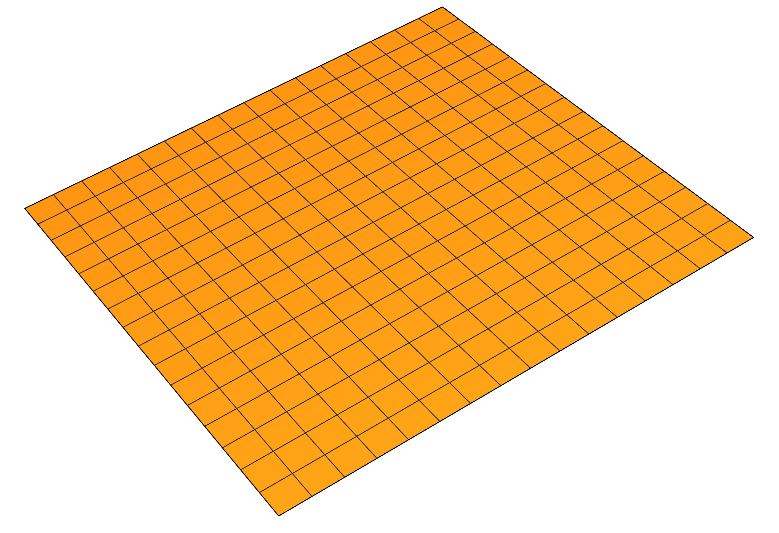
\includegraphics[width=\textwidth]{picture/week4/plane.pdf}
    \caption{Plane}
\end{subfigure}
\begin{subfigure}{0.2\textwidth}
    \centering
    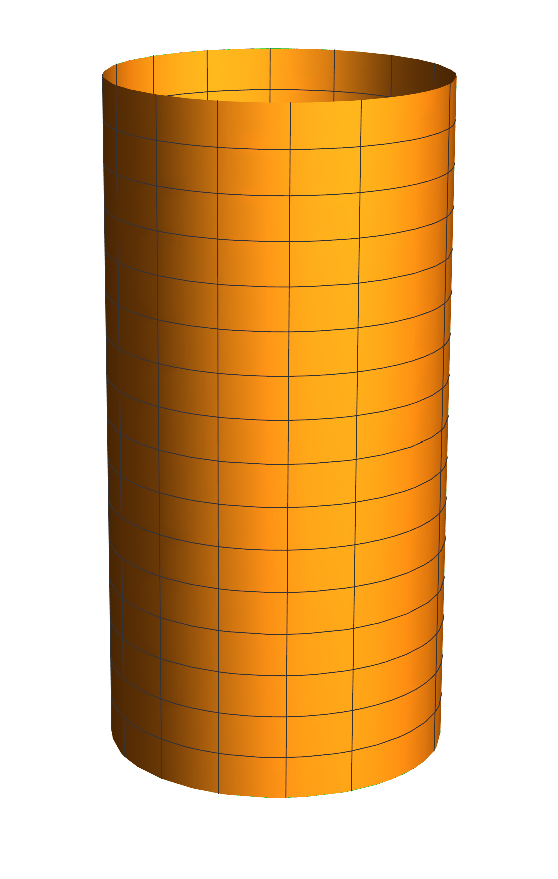
\includegraphics[width=\textwidth]{picture/week4/cylinder.pdf}
    \caption{Cylinder}
\end{subfigure}
\begin{subfigure}{0.4\textwidth}
    \centering
    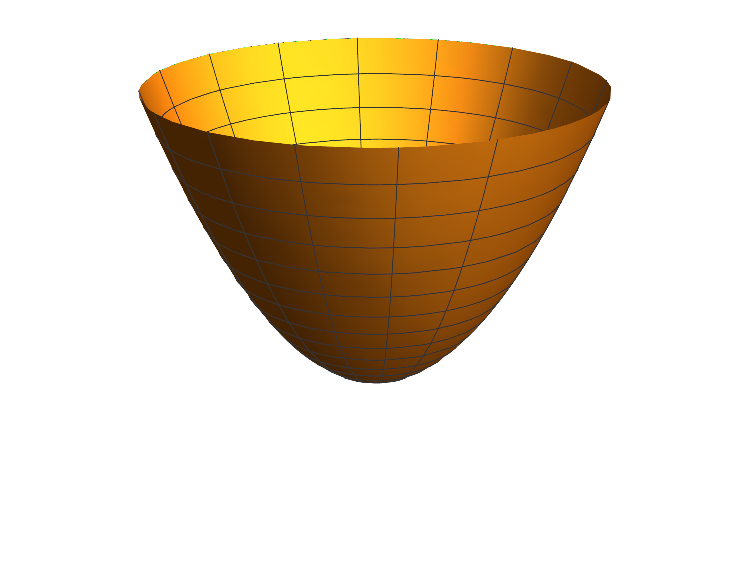
\includegraphics[width=\textwidth]{picture/week4/paraboloid.pdf}
    \caption{Paraboloid}
\end{subfigure}
\begin{subfigure}{0.3\textwidth}
    \centering
    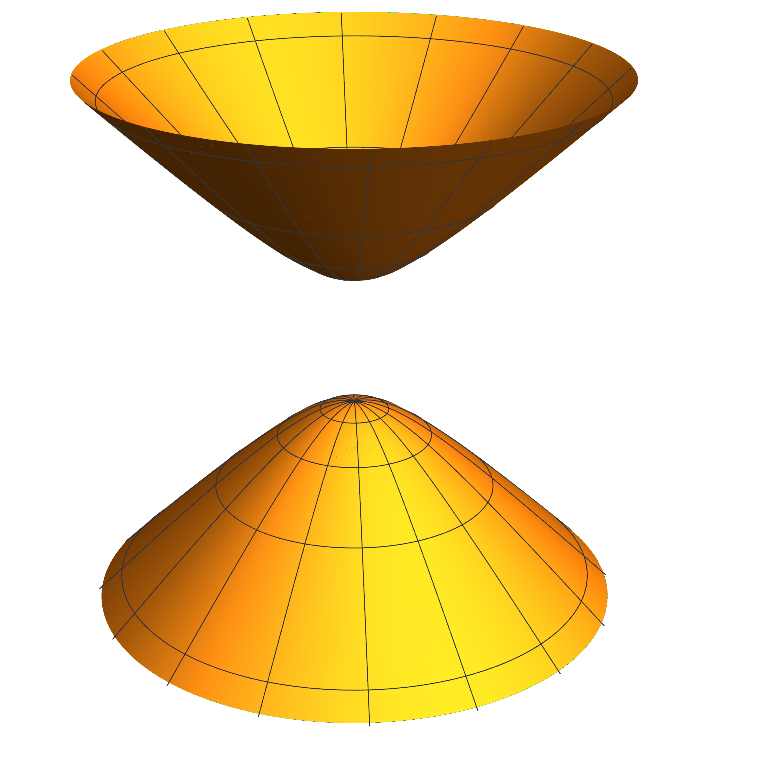
\includegraphics[width=\textwidth]{picture/week4/hyperboloid.pdf}
    \caption{Hyperboloid}
\end{subfigure}
\begin{subfigure}{0.2\textwidth}
    \centering
    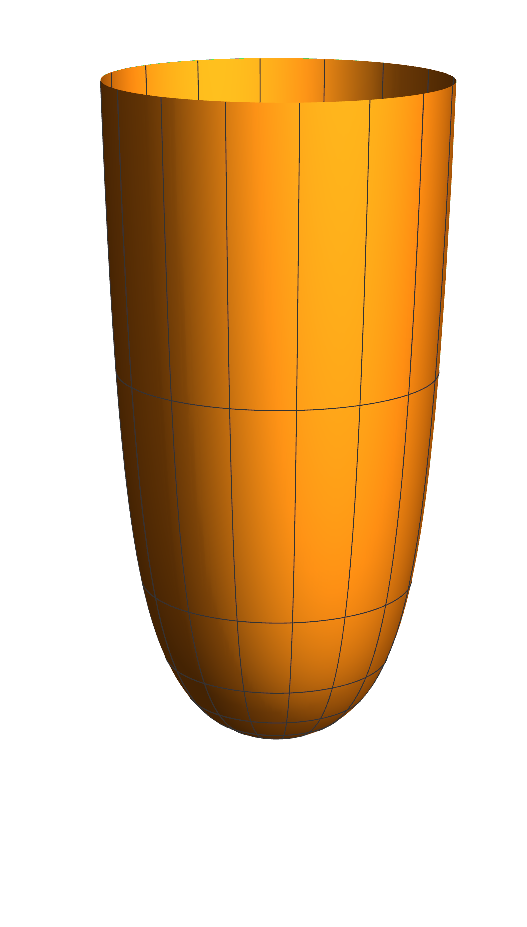
\includegraphics[width=\textwidth]{picture/week4/cigar.pdf}
    \caption{Cigar soliton}
\end{subfigure}
\caption*{Surface collection 1}
\end{figure}

\begin{figure}
\centering
\begin{subfigure}{0.25\textwidth}
    \centering
    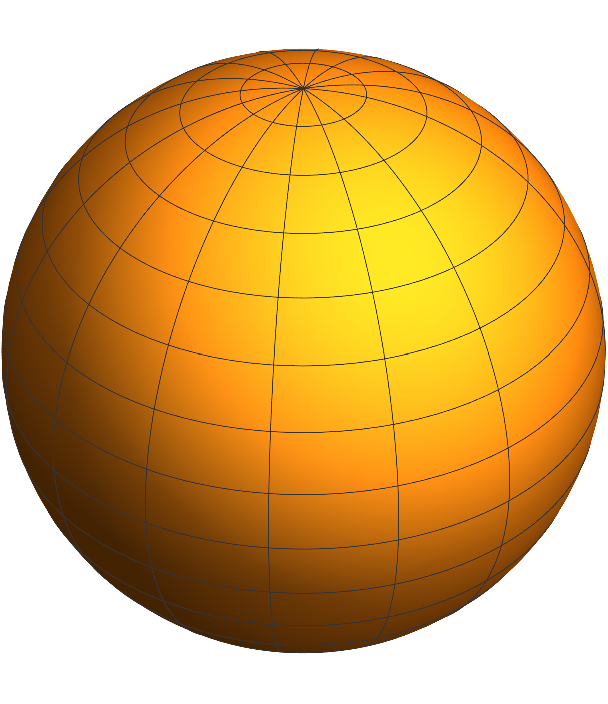
\includegraphics[width=\textwidth]{picture/week4/sphere.pdf}
    \caption{\(\mathbb{S}^2\)}
\end{subfigure}
\begin{subfigure}{0.35\textwidth}
    \centering
    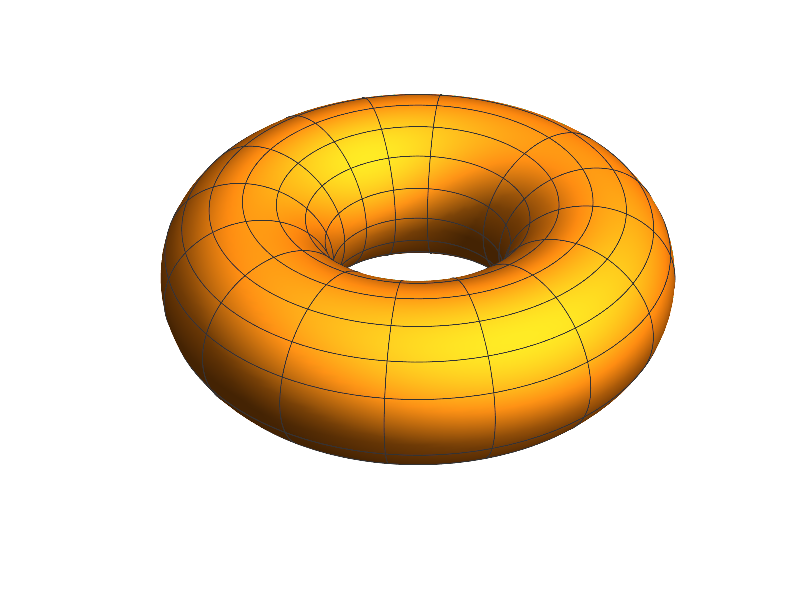
\includegraphics[width=\textwidth]{picture/week4/torus.pdf}
    \caption{\(\mathbb{T}^2\)}
\end{subfigure}
\begin{subfigure}{0.35\textwidth}
    \centering
    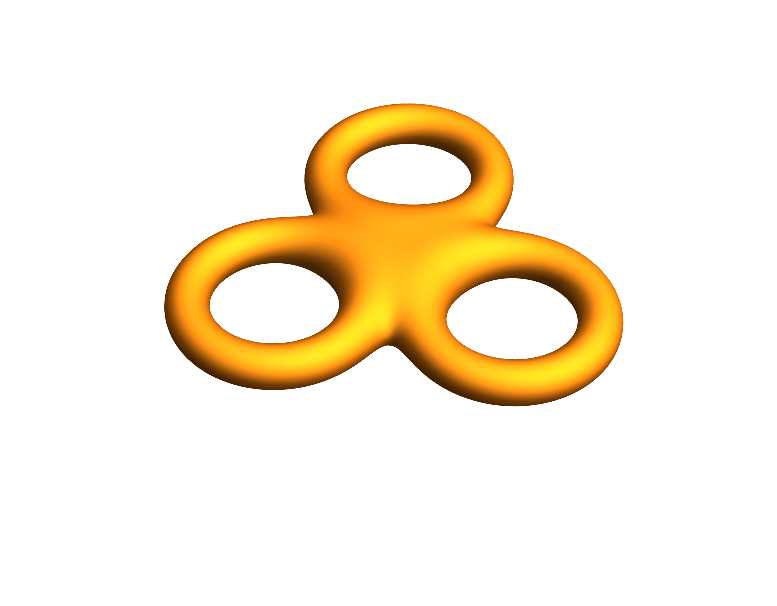
\includegraphics[width=\textwidth]{picture/week4/torus3.pdf}
    \caption{\(\Sigma_g\) for \(g=3\)}
\end{subfigure}
\caption*{Surface collection 2}
\end{figure}

\begin{figure}
\centering
\begin{subfigure}{0.45\textwidth}
    \centering
    
\includegraphics[width=\textwidth]{picture/week4/helicoid.pdf}
    \caption{Helicoid}
\end{subfigure}
\begin{subfigure}{0.45\textwidth}
    \centering
    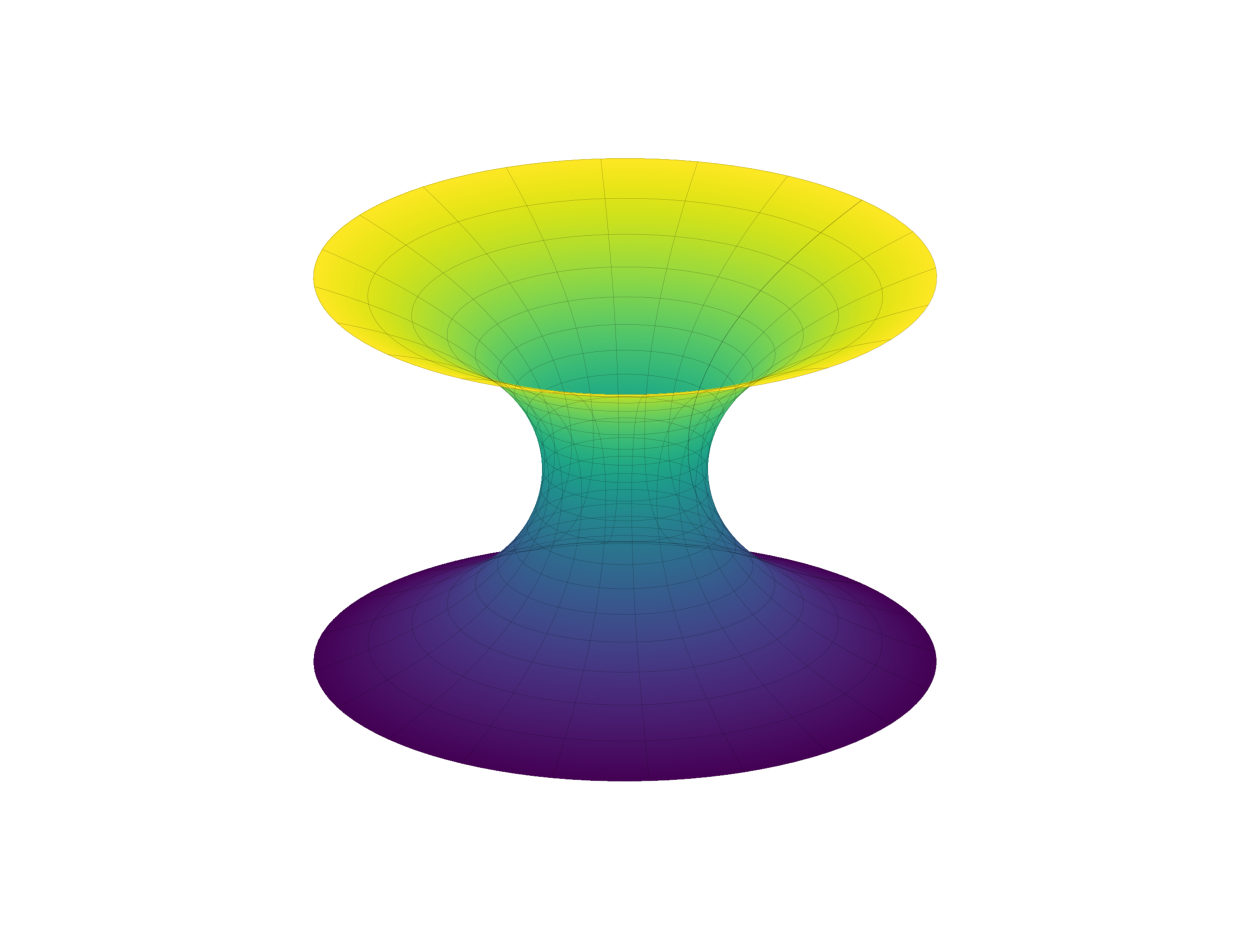
\includegraphics[width=\textwidth]{picture/week4/catenoid.pdf}
    \caption{Catenoid}
\end{subfigure}
\begin{subfigure}{0.5\textwidth}
    \centering
    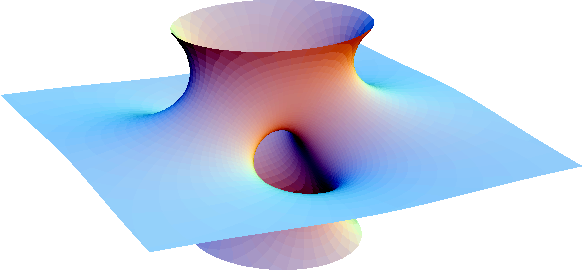
\includegraphics[width=\textwidth]{picture/week4/costa.pdf}
    \caption{Costa minimal surface}
\end{subfigure}
\begin{subfigure}{0.4\textwidth}
    \centering
    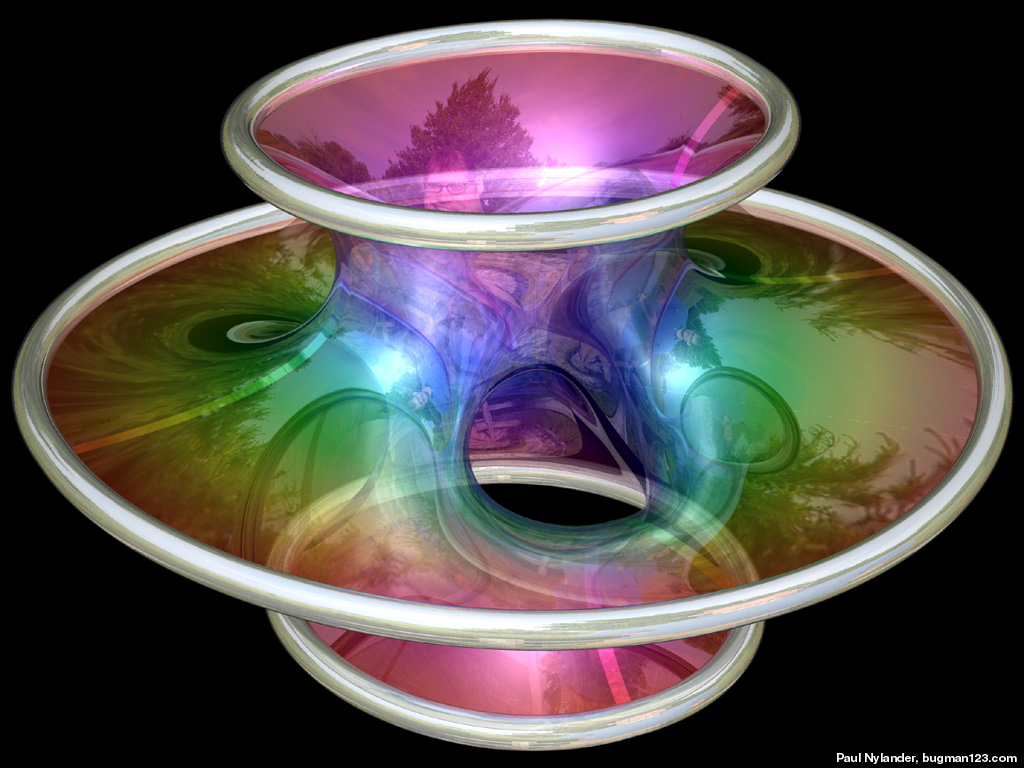
\includegraphics[width=\textwidth]{picture/week4/Costa-large.jpg}
    \caption{Soap bubble}
\end{subfigure}
\caption*{Surface collection 3}
\end{figure}

\begin{figure}
\centering
\begin{subfigure}{0.3\textwidth}
    \centering
    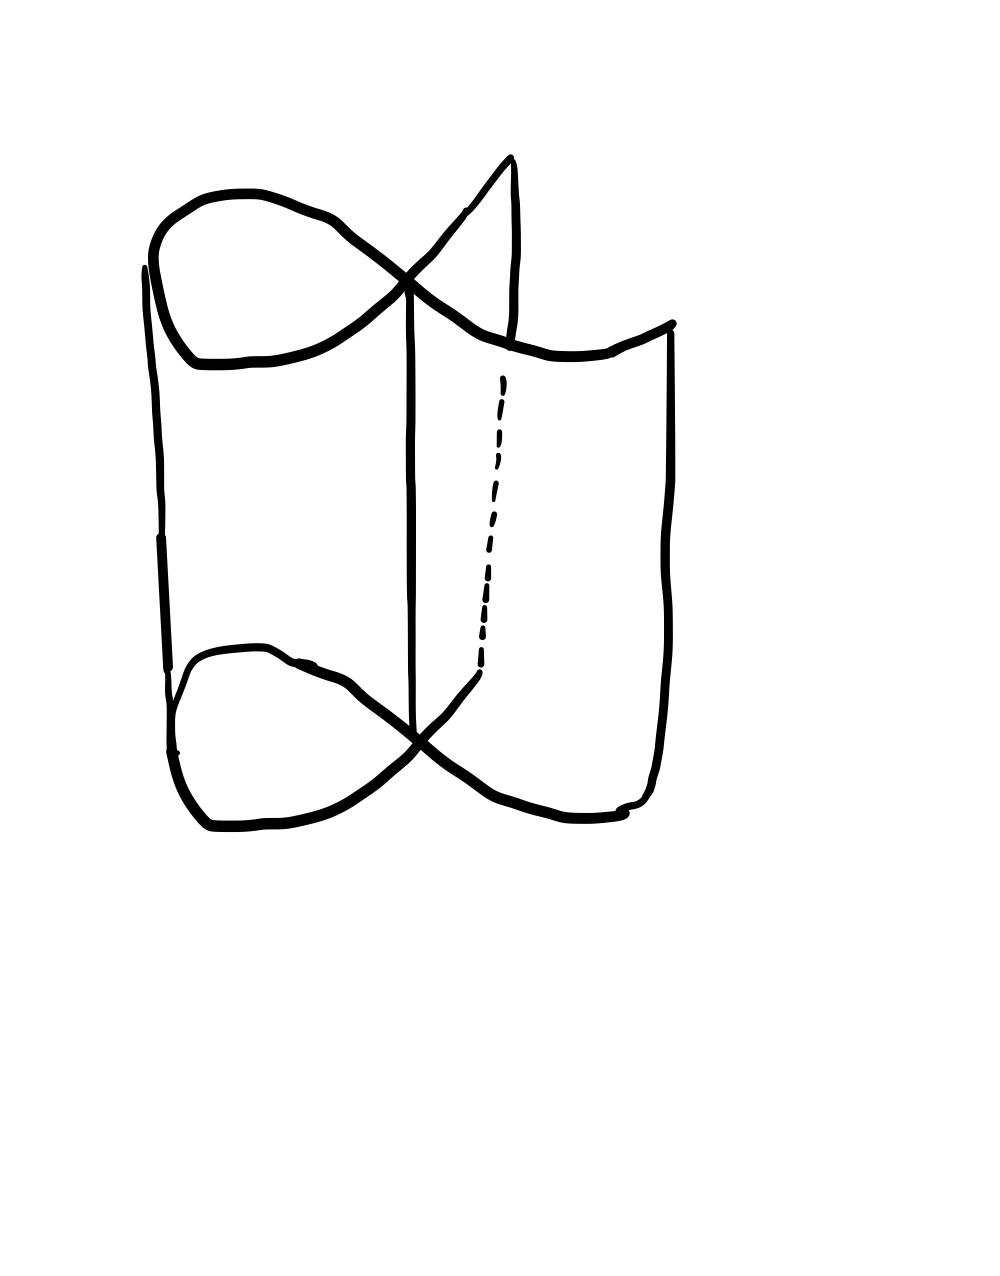
\includegraphics[width=\textwidth]{picture/week4/self-intersetcion.png}
    \caption{Self-intersected}
\end{subfigure}
\begin{subfigure}{0.35\textwidth}
    \centering
    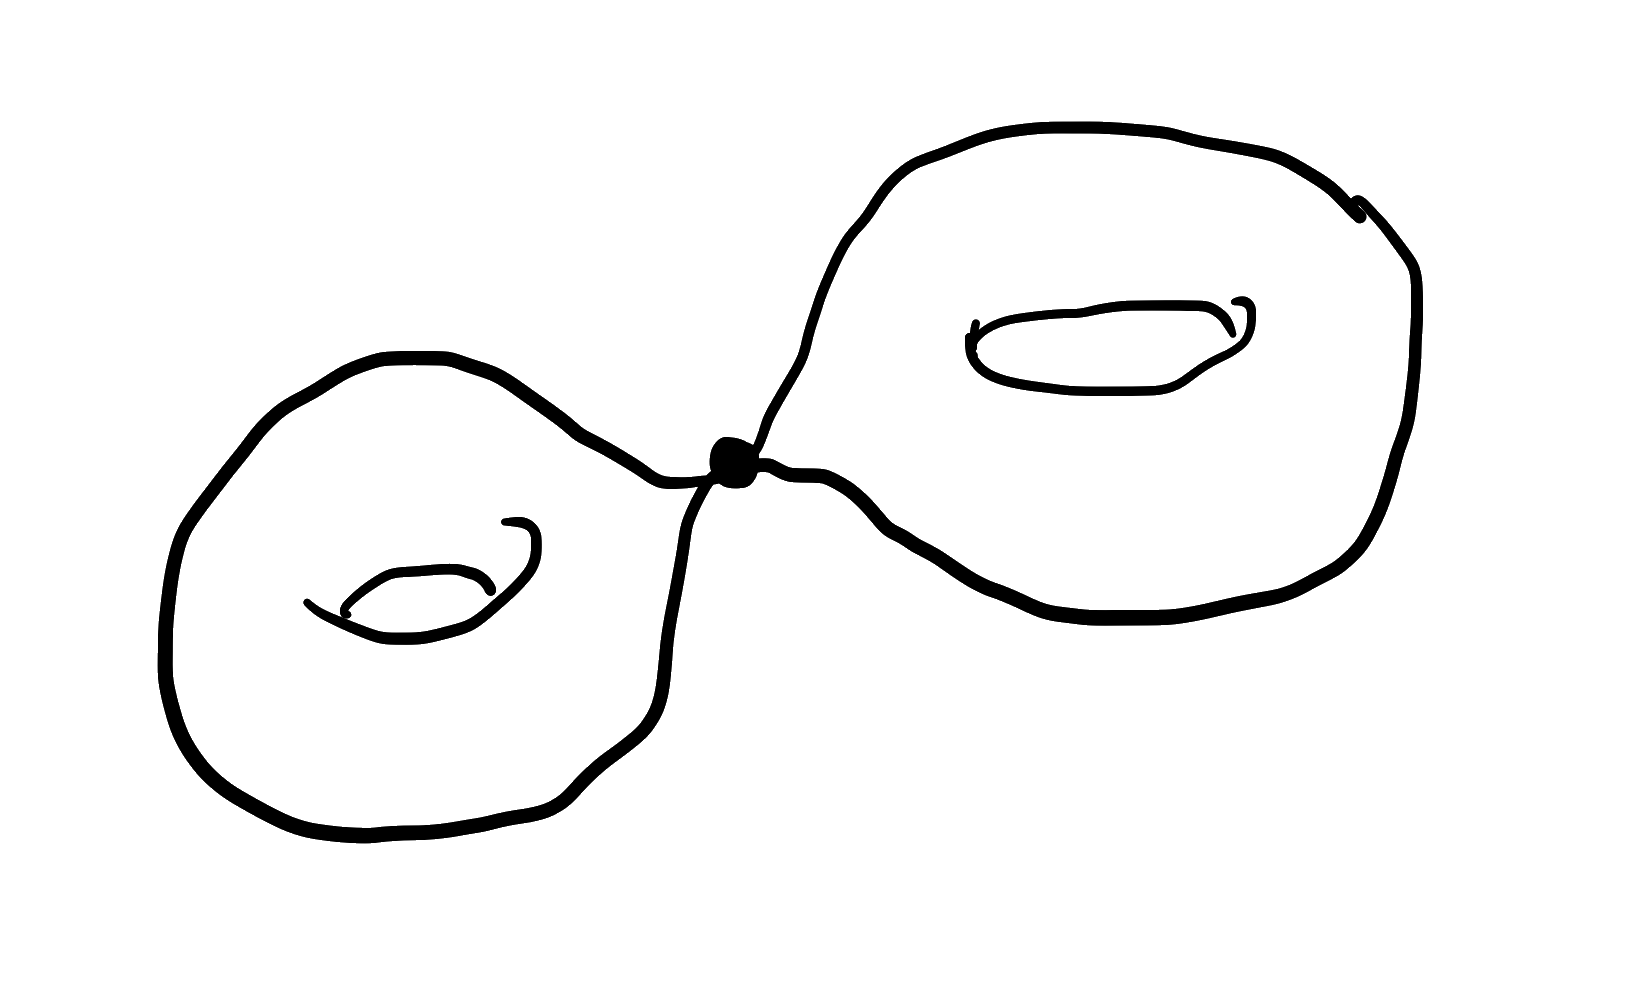
\includegraphics[width=\textwidth]{picture/week4/node.png}
    \caption{Nodal surfaces}
\end{subfigure}
\begin{subfigure}{0.3\textwidth}
    \centering
    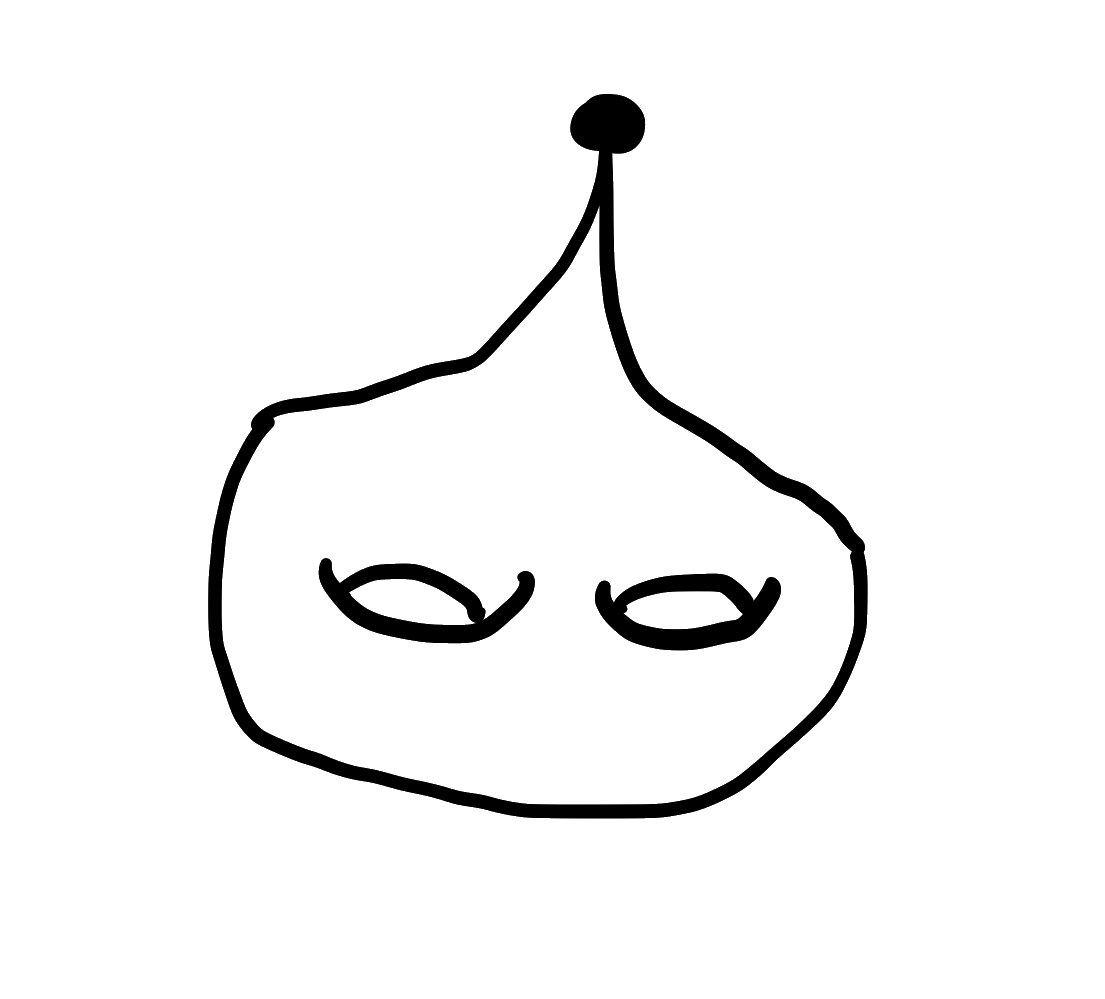
\includegraphics[width=\textwidth]{picture/week4/cusp.png}
    \caption{Cusp}
\end{subfigure}
\caption*{``Surface'' collection 4}
\end{figure}

\begin{example}\hfill
\begin{itemize}
    \item Collection 1 are complete non-compact surfaces.
    \item Collection 2 are compact surfaces without boundary (closed).
    \item Collection 3 are so called minimal surfaces, a very important class
        of surfaces. The term ``minimal'' intuits smallest area in certain sense.
    \item There are surfaces will NOT be investigated in this course, the ones with
        self-intersection, node points or cusps, and non-orientable surfaces.
\end{itemize}    
\end{example}

\section{Definition of Regular Surface}

\begin{definition}[Regular surfaces in \(\mathbb{R}^3\)]\hfill\par
    A subset \(S\subset \mathbb{R}^3\) is called a regular surface, if \(\forall\,p
    \in S\), \(\exists\, V\subset\mathbb{R}^3\) neighborhood of \(p\), an open set
    \(U\subset \mathbb{R}^2\) and a trivialization map \[
        F\colon U\to V\cap S
    .\] \st\ \(F\) is smooth, homeomorphism onto its image, and regular.
\end{definition}
\begin{remark}\hfill
\begin{enumerate}[(1)]
    \item \(F\) is homeomorphism means both \(F\) and \(F^{-1}\) are continuous map.
    \item \(F\) is ``regular'' means \(\forall\,p\in U\), \(\dif F_p\) is an 
        injection as linear map \(\mathbb{R}^2\to \mathbb{R}^3\).
\end{enumerate}
\end{remark}

Let's see what the term ``regular'' means:

Assume \(F\) is written as \(F(u,v)=(x(u,v),y(u,v),z(u,v))\), at \(p\in U\), \[
    \dd{F_p}\colon T_p U\to T_{F(p)}S
\] is a linear map. On \(\mathbb{R}^2\), coordinate vector fields \(\{\pdv{u},
\pdv{v}\}\) form a basis. On \(\mathbb{R}^3\) we also have standard basis
\(\{\pdv{x},\pdv{y},\pdv{z}\}\). Then \[
    \dd{F_p}\begin{bmatrix}
        \pdv{u}\\ \pdv{v}
    \end{bmatrix}
    =\begin{bmatrix}
        \pdv{x}{u} & \pdv{y}{u} & \pdv{z}{u} \\ 
        \pdv{x}{v} & \pdv{y}{v} & \pdv{z}{v}
    \end{bmatrix}
    \begin{bmatrix}
        \pdv{x}\\ \pdv{y}\\ \pdv{z}
    \end{bmatrix}
.\] Hence
\begin{align*}
    \dd{F_p}\text{ is injective}
    \iff & \ker\dd{F_p}=0 \\
    \iff & \pdv{(x,y,z)}{(u,v)}\text{ has rank 2} \\
    \iff & \pdv{F}{u}\text{ \& }\pdv{F}{v}\text{ are linearly independent} \\
    \iff & \pdv{F}{u}\times \pdv{F}{v}\neq 0. \\
    & \text{\small\itshape\/ (Geometrically this defines the normal vector field} \\
    & \text{\small\itshape\/ of the tangent plane)} \\
    \iff & \text{ One of the following minors is non-zero:}\\
    & \quad\left|\pdv{(x,y)}{(u,v)}\right|,\quad\left|\pdv{(x,z)}{(u,v)}\right|,
    \quad\left|\pdv{(y,z)}{(u,v)}\right|
\end{align*}
{\small\itshape
    (Geometrically, this means \((u,v)\) can be viewed as coordinate at \(p\in S\)
    via \(F\). In fact, since ``\(\dd{F_p}\) is injective'' is an open condition,
    \((u,v)\) serves as a local coordinate chart in a neighborhood of \(p\))
}

We also call \(F\) to be a local parametrization of \(S\). Note that such \(F\)
is usually not globally defined.

From the definition, we see a regular surface in \(\mathbb{R}^3\) is characterized
by at each point, we can find a ``smooth'' slice chart in a neighbourhood of the
point. The term ``slice chart'' means coordinate chart with local part of the
surface containing in the chart as a slice.

\begin{question}
    Consider two points \(p,q\) on the surface, live close to each other. It might
    happen that their corresponding coordinate chart overlap. Then in the
    intersection of two charts, there are two different parametrizations. What
    relation between these two parametrizations should be?
\end{question}
% Figure here

Set-up: \(F_1\colon U_1\to V_1\cap S,\ (u,v)\mapsto F_1(u,v)\),\hfill \(F_2\colon
U_2\to V_2\cap S,\ (\alpha,\beta)\mapsto F_2(\alpha,\beta)\)

Let \(W=V_1\cap V_2\cap S\), since \(F_i\) is homeomorphism, \(F_1^{-1}(W)\subset U,
\ F_2^{-1}(W)\subset U_2\).

\noindent\underline{\textbf{Claim:}} (Very important).\par
\(G=F_2^{-1}\circ F_1\colon F_1^{-1}(W)\to F_2^{-1}(W)\) is a diffeomorphism,\ie\ 
both \(G\) and \(G^{-1}\) are smooth functions.

The importance of this claim leads us to give an intrinsic definition of a regular
surface \(S\). \ie\ a regular surface is obtained by padding up open sets in
\(\mathbb{R}^2\), in a smooth way. Later in differential geometry course, we'll
define a smooth manifold by such intrinsic definition. The diffeomorphism \(G\)
above is called the transition map. Different property of \(G\) determines different
structure. If \(G\) is only a homeomorphism, then \(S\) is a topological surface.
If \(G\) is a bi-holomorphism, then \(S\) is a complex surface.

The proof of the claim needs the inverse function theorem.
\begin{theorem}[Inverse function thm]
    \(U\subset \mathbb{R}^n\) open. \(F\colon U\to \mathbb{R}^n\) is a \(C^1\) map,
    \(p\in U\). If \(\dd{F_p}\colon \mathbb{R}^n\to \mathbb{R}^n\) is an isomorphism,
    then there is a neighbourhood of \(p\) and a neighbourhood of \(F(p)\).
    \st\ \(F\colon V\to W\) is invertible. Moreover \(F^{-1}\) is also \(C^1\). If
    condition is substituted to \(F\) smooth, then \(F^{-1}\) has same smoothness.
\end{theorem}

\begin{remark}
    From linear algebra, a linear operator on finite dimensional vector space
    is injective iff it's surjective. Hence it's sufficient to check \(\det(\dd{F_p})
    \neq 0\), \ie\ \(\dd{F_p}\) is non-singular.
\end{remark}

\textbf{\color{red}!!} Apriori, we don't know if \(F_2^{-1}\) is smooth, since we
have not defined what ``smooth map'' on a surface mean.

\begin{proof}[Proof of claim]
    Since \(F_1\) and \(F_2\) are homeomorphism, \(G,G^{-1}\) are continuous.
    \(S\) is a regular surface, so at \(p\in U_1\), \((\dd{F_1})_p\colon\mathbb{R}^2
    \to \mathbb{R}^3\) is injective. W.L.O.G. we can assume \[
        \left|\pdv{(x,y)}{(u,v)}\right|\neq 0\text{ at }p
    .\] Consider a map \(h\colon F_1^{-1}(W)\times (-\eps,\eps)\to \mathbb{R}^3,
    (u,v,t)\mapsto (x(u,v),y(u,v),z(u,v)+t)\). Then \(h\) has Jacobian \[
        \det \begin{bmatrix}
            x_u & y_u & z_u \\
            x_v & y_v & z_v \\
            0 & 0 & 1
        \end{bmatrix}
        =\det\begin{bmatrix}
            x_u & y_u \\
            x_v & y_v 
        \end{bmatrix}\neq 0 \text{ at }p
    .\] By inverse function theorem, \(\exists\) a neighbourhood \(D\subset
    \mathbb{R}^3\) of \((p,t)\) \st\ \(h\) is invertible on \(D\), and \(h^{-1}\)
    smooth. Now since \(F_1^{-1}\circ F_2=\eval{h^{-1}\circ F_2}_{t=0}\), and RHS
    is smooth, we conclude that \(F_1^{-1}\circ F_2\) is smooth. Similarly \(G^{-1}\)
    is smooth.
\end{proof}

Now we give an intrinsic definition (No need to assume \(S\subset \mathbb{R}^3\)).
\begin{definition}
    Topological space \(S\) (second countable, Hausdorff) is called a regular surface
    if \(S\) has a covering \(\{V_\alpha,f_\alpha\}\) \st\ 
    \begin{enumerate}[(1)]
        \item \(f_\alpha\colon V_\alpha\to f_\alpha(V_\alpha)\overset{\text{open}}
            \subset \mathbb{R}^2\) is a homeomorphism.
        \item If \(V_\alpha\cap V_\beta\neq \emptyset\), then \[
            f_\beta\circ f_\alpha^{-1}\colon f_\alpha(v_\alpha\cap V_\beta)\to 
            f_\beta(V_\alpha\cap V_\beta)
        \] is a diffeomorphism, called the transition map.
    \end{enumerate}
\end{definition}
\begin{remark}
    In higher dimension, this definition yields ``smooth manifold''.
\end{remark}

\section{Examples of Regular Surfaces}

\begin{example}[1]
    \(\mathbb{R}^2\hookrightarrow\mathbb{R}^3\) is a regular surface with (trivial)
    global parametrization \[
        F(x,y)=(x,y,0)
    .\] 
\end{example}

\begin{example}[2]
    Standard 2-sphere \(\mathbb{S}^2=\{(x,y,z):x^2+y^2+z^2=1\}\). This is a very
    important example, we'll give (local) parametrization for \(\mathbb{S}^2\)
    in 3 ways.
\end{example}
\noindent (a) Parametrization induced from \(\mathbb{R}^3\).

If the point is on upper hemisphere, let \(U=\{x^2+y^2<1\}\), \[
    F_1\colon U\to \mathbb{S}^2,\ (x,y)\mapsto (x,y,\sqrt{1-x^2-y^2}).
\] Check definition:

\(F_1\) is smooth \checkmark{}. 

\(F_1\colon U\to F_1(U)\) is homeomorphism, since \(F_1^{-1}\) is
projection onto \(xy\)-plane, is also continuous.

\(F_1\) is regular: \[
    \pdv{F_1}{x}=(1,0,-\frac{x}{\sqrt{1-x^2-y^2}}),\quad
    \pdv{F_1}{y}=(0,1,-\frac{y}{\sqrt{1-x^2-y^2}})
.\] Clearly they are linearly independent.

Similarly, if the point is on lower hemisphere, we have \[
    F_2\colon U\to \mathbb{S}^2,\ (x,y)\mapsto (y,x,-\sqrt{1-x^2-y^2})
.\] However, \(F_1(U)\cup F_2(U)\) can not fully cover \(\mathbb{S}^2\), points on
the equator are left. To cover them, we add 4 more charts:
\begin{align*}
    F_3(y,z)&= (\sqrt{1-y^2-z^2},y,z) &&\text{(front hemisphere)} \\
    F_4(y,z)&= (-\sqrt{1-y^2-z^2},z,y) &&\text{(back)} \\
    F_5(z,x)&= (x,\sqrt{1-x^2-z^2},z) &&\text{(right)} \\
    F_6(z,x)&= (z,-\sqrt{1-x^2-z^2},x) &&\text{(left)}
\end{align*}
We can check \(F_2\)-\(F_6\) also satisfy the definition. Hence we have given each
point a smooth chart, and \(\mathbb{S}^2\) is regular.
\begin{exercise}
    Check transition maps between \(F_1\)-\(F_6\) are smooth.
\end{exercise}

\noindent (b) Geographical parametrization.

% Maybe picture here
Let \(U=\{(\theta,\vphi)\in \mathbb{R}^2:0<\theta<2\pi,0<\vphi<\pi\}\), 
\begin{align*}
    &F_1\colon U\to \mathbb{S}^2,\ (\theta,\vphi)\mapsto 
    (\cos\theta\sin\vphi,\sin\theta\sin\vphi,\cos\vphi)
    \quad\text{(missing half of }\{y=0\}\cap \mathbb{S}^2\text{)}\\ 
    &F_2\colon U\to \mathbb{S}^2,\ (\theta,\vphi)\mapsto 
    (\sin\theta\sin\vphi,\cos\vphi,\cos\theta\sin\vphi)
    \quad\text{(missing half of }\{x=0\}\cap \mathbb{S}^2\text{)}\\ 
    &F_3\colon U\to \mathbb{S}^2,\ (\theta,\vphi)\mapsto 
    (\cos\vphi,\cos\theta\sin\vphi,\sin\theta\sin\vphi)
    \quad\text{(missing half of }\{z=0\}\cap \mathbb{S}^2\text{)}
.\end{align*}
Clearly \(\mathbb{S}^2\subset F_1(U)\cup F_2(U)\cup F_3(U)\), each \(F_i\) is smooth
and regular. To see they are homeomorphism, we can compute e.g. \[
    F_1^{-1}(x,y,z)=(\arccos \frac{x}{\sqrt{x^2+y^2}}, \arccos z)
.\] 

\noindent (c) Stereographical parametrization.

Consider the ray connecting north pole \((0,0,1)\) and point \((x,y,z)\) on
\(\mathbb{S}^2\). Then there is a unique point \((u,v)\) on \(xy\)-plane on the
ray, the projection is given by \[
    p_N\colon \mathbb{S}^2\setminus\{N\}\to \mathbb{R}^2,
    \quad (x,y,z)\mapsto (\frac{x}{1-z},\frac{y}{1-z})=\colon(u,v)
\] which is rational map, with inverse \[
    p_N^{-1}(u,v)=(\frac{2u}{1+u^2+v^2},\frac{2v}{1+u^2+v^2},1-\frac{2}{1+u^2+v^2})
\] also rational and normal.

\section{Differential Functions on a regular surface}
\begin{question}[1]
    How to define a function on $\mathbb{S}^2$?
\end{question}
In calculus, we have seen this is just $f\left(x,y,z
    \right)|_{\mathbb{S}^2}$, but what does this mean?
If $p\in $ upper half semi-sphere $\Rightarrow$ $f\left(x,y,\sqrt{1-x^2-y^2}\right)$ $\Rightarrow f$ is just a function on
\[
    U={(x,y)\in \mathbb{R}^3\colon x^2+y^2<1}  .
\]

More precisely, if we let $F\colon U\to \mathbb{S}^2$ be the local parametrization,
\[
    (x,y)\mapsto (x,y,\sqrt{1-x^2-y^2}),
\]
then $\tilde{f}(x,y)\colon U\to \mathbb{R}, \tilde{f}(x,y)=f\circ  F$.

Similarly, if the point lies on other five charts(see \cref{charts on unit sphere}). There is also a function $\tilde{f}$ essentially defined on an open set of $\mathbb{R}^2$ to associate $f$.

\begin{question}[2]
    What does it mean by a ``smooth'' (or differentiable) function on $\mathbb{S}^2$?
\end{question}
\begin{align*}
    f \text{ is smooth near }p \Leftrightarrow &
    \tilde{f}\colon U\subset \mathbb{R}^2 \to \mathbb{R} \text{is smooth,}                                                 \\
                                               & (\because F\colon U\subset \mathbb{R}^2\to \mathbb{S}^2 \text{is smooth})
\end{align*}
\begin{question}[3]
    $p$ could lie on two charts, (\ie\ we can associate two coordinate charts near $p$, will the ``smoothness'' of $f$ be affected?)
\end{question}

\tikzset{every picture/.style={line width=0.75pt}} %set default line width to 0.75pt        

\begin{tikzpicture}[x=0.75pt,y=0.75pt,yscale=-0.9,xscale=0.9]
    %uncomment if require: \path (0,300); %set diagram left start at 0, and has height of 300

    %Shape: Axis 2D [id:dp5905610283034792] 
    \draw  (128,153) -- (228,153)(138,63) -- (138,163) (221,148) -- (228,153) -- (221,158) (133,70) -- (138,63) -- (143,70)  ;
    %Straight Lines [id:da5258527733857374] 
    \draw    (146,144) -- (74.76,221.03) ;
    \draw [shift={(73.4,222.5)}, rotate = 312.76] [color={rgb, 255:red, 0; green, 0; blue, 0 }  ][line width=0.75]    (10.93,-3.29) .. controls (6.95,-1.4) and (3.31,-0.3) .. (0,0) .. controls (3.31,0.3) and (6.95,1.4) .. (10.93,3.29)   ;
    %Shape: Circle [id:dp7596976921705518] 
    \draw   (74.8,153) .. controls (74.8,118.1) and (103.1,89.8) .. (138,89.8) .. controls (172.9,89.8) and (201.2,118.1) .. (201.2,153) .. controls (201.2,187.9) and (172.9,216.2) .. (138,216.2) .. controls (103.1,216.2) and (74.8,187.9) .. (74.8,153) -- cycle ;
    %Shape: Arc [id:dp4458065415749495] 
    \draw  [draw opacity=0] (200.4,152.37) .. controls (200.4,152.37) and (200.4,152.37) .. (200.4,152.37) .. controls (200.4,169.01) and (172.28,182.5) .. (137.6,182.5) .. controls (102.92,182.5) and (74.8,169.01) .. (74.8,152.37) -- (137.6,152.37) -- cycle ; \draw   (200.4,152.37) .. controls (200.4,152.37) and (200.4,152.37) .. (200.4,152.37) .. controls (200.4,169.01) and (172.28,182.5) .. (137.6,182.5) .. controls (102.92,182.5) and (74.8,169.01) .. (74.8,152.37) ;
    %Shape: Arc [id:dp1079879229191647] 
    \draw  [draw opacity=0][dash pattern={on 4.5pt off 4.5pt}] (74.8,152.37) .. controls (74.8,152.37) and (74.8,152.37) .. (74.8,152.37) .. controls (74.8,135.74) and (102.92,122.25) .. (137.6,122.25) .. controls (172.28,122.25) and (200.4,135.74) .. (200.4,152.37) -- (137.6,152.37) -- cycle ; \draw  [dash pattern={on 4.5pt off 4.5pt}] (74.8,152.37) .. controls (74.8,152.37) and (74.8,152.37) .. (74.8,152.37) .. controls (74.8,135.74) and (102.92,122.25) .. (137.6,122.25) .. controls (172.28,122.25) and (200.4,135.74) .. (200.4,152.37) ;
    %Shape: Circle [id:dp8215567727809696] 
    \draw  [fill={rgb, 255:red, 67; green, 243; blue, 243 }  ,fill opacity=0.7 ] (136.48,118.05) .. controls (127.92,110.28) and (128.47,102.27) .. (137.71,100.15) .. controls (146.96,98.03) and (161.39,102.61) .. (169.95,110.38) .. controls (178.51,118.14) and (177.96,126.16) .. (168.71,128.27) .. controls (159.47,130.39) and (145.04,125.81) .. (136.48,118.05) -- cycle ;
    %Shape: Ellipse [id:dp5973540554680155] 
    \draw  [fill={rgb, 255:red, 182; green, 250; blue, 18 }  ,fill opacity=0.7 ] (153.21,114.21) .. controls (156.92,108.46) and (161.1,114.64) .. (162.55,128) .. controls (164.01,141.36) and (162.19,156.86) .. (158.49,162.6) .. controls (154.79,168.35) and (150.6,162.18) .. (149.15,148.81) .. controls (147.69,135.45) and (149.51,119.96) .. (153.21,114.21) -- cycle ;
    %Shape: Circle [id:dp24020151067783413] 
    \draw  [fill={rgb, 255:red, 0; green, 0; blue, 0 }  ,fill opacity=1 ] (155,119.75) .. controls (155,118.51) and (156.01,117.5) .. (157.25,117.5) .. controls (158.49,117.5) and (159.5,118.51) .. (159.5,119.75) .. controls (159.5,120.99) and (158.49,122) .. (157.25,122) .. controls (156.01,122) and (155,120.99) .. (155,119.75) -- cycle ;
    %Shape: Axis 2D [id:dp6541206749950883] 
    \draw  (273,93.05) -- (400.4,93.05)(323.2,11.5) -- (323.2,136) (393.4,88.05) -- (400.4,93.05) -- (393.4,98.05) (318.2,18.5) -- (323.2,11.5) -- (328.2,18.5)  ;
    %Shape: Polygon Curved [id:ds3396588391090478] 
    \draw  [fill={rgb, 255:red, 67; green, 243; blue, 243 }  ,fill opacity=0.7 ] (323.4,36.5) .. controls (343.4,26.5) and (380.4,10.5) .. (392.4,28.5) .. controls (394.54,31.71) and (396.35,34.97) .. (397.81,38.22) .. controls (404.56,53.16) and (404.05,67.85) .. (395.4,76.5) .. controls (386.1,85.8) and (391.98,80.62) .. (356.01,83.08) .. controls (351.25,83.4) and (345.76,83.86) .. (339.4,84.5) .. controls (285,90) and (303.4,46.5) .. (323.4,36.5) -- cycle ;
    %Shape: Axis 2D [id:dp15349087590497468] 
    \draw  (232,218.15) -- (360.4,218.15)(291.87,142.5) -- (291.87,279) (353.4,213.15) -- (360.4,218.15) -- (353.4,223.15) (286.87,149.5) -- (291.87,142.5) -- (296.87,149.5)  ;
    %Shape: Polygon Curved [id:ds9697525934649356] 
    \draw  [fill={rgb, 255:red, 182; green, 250; blue, 18 }  ,fill opacity=0.7 ] (254.4,215.5) .. controls (285.4,172.5) and (341.4,177.5) .. (347,206) .. controls (352.6,234.5) and (333.8,284) .. (293.4,257.5) .. controls (253,231) and (223.4,258.5) .. (254.4,215.5) -- cycle ;
    %Curve Lines [id:da20815011674520578] 
    \draw    (283.4,52.5) .. controls (241.82,39.63) and (218.86,41.46) .. (196.09,81.28) ;
    \draw [shift={(195.4,82.5)}, rotate = 299.29] [color={rgb, 255:red, 0; green, 0; blue, 0 }  ][line width=0.75]    (10.93,-3.29) .. controls (6.95,-1.4) and (3.31,-0.3) .. (0,0) .. controls (3.31,0.3) and (6.95,1.4) .. (10.93,3.29)   ;
    %Curve Lines [id:da056699720507130014] 
    \draw    (233.4,247.5) .. controls (212.82,252.4) and (178.79,248.66) .. (161.44,224.97) ;
    \draw [shift={(160.4,223.5)}, rotate = 55.78] [color={rgb, 255:red, 0; green, 0; blue, 0 }  ][line width=0.75]    (10.93,-3.29) .. controls (6.95,-1.4) and (3.31,-0.3) .. (0,0) .. controls (3.31,0.3) and (6.95,1.4) .. (10.93,3.29)   ;

    % Text Node
    \draw (428,41.4) node [anchor=north west][inner sep=0.75pt]    {$ \begin{array}{l}
                \tilde{f}( x,y) =f\circ F_{1} \\
                \ \ \ \ \ \ \ \ \ \ \ =f\left( x,y,\sqrt{1-x^{2} -y^{2}}\right)
            \end{array}$};
    % Text Node
    \draw (408,177.4) node [anchor=north west][inner sep=0.75pt]    {$ \begin{array}{l}
                \tilde{f}( x,z) =f\circ F_{2} \\
                \ \ \ \ \ \ \ \ \ \ \ =f\left( x,\sqrt{1-x^{2} -z^{2}} ,z\right)
            \end{array}$};
    % Text Node
    \draw (210,22.4) node [anchor=north west][inner sep=0.75pt]    {$F_{1}$};
    % Text Node
    \draw (188,223.4) node [anchor=north west][inner sep=0.75pt]    {$F_{2}$};
    % Text Node
    \draw (351,45.4) node [anchor=north west][inner sep=0.75pt]    {$U_{1}$};
    % Text Node
    \draw (305,237.4) node [anchor=north west][inner sep=0.75pt]    {$U_{2}$};


\end{tikzpicture}

Smoothness is not affected by the coordinate change. Moreover, it's easy to
apply the chain rule to find relation of differentials of f between
different coordinate charts.
\begin{definition}[Differential function]
    $S$ is a regular surface in $\mathbb{R}^3$. A function $f$ is said to
    be differentiable at $p\in S$, if for a local parametrization near $p$
    \[
        x\colon U\subset \mathbb{R}^2\to \mathbb{R}^3,
    \]
    the function $f\circ x\colon \mathbb{R}^2\to \mathbb{R}$ is
    differentiable at $x^{-1}(p)$
\end{definition}
\begin{remark}
    $f\circ x$ is well-defined, since the differentiability is not affected
    by a change of parameter, e.g. if $y\colon V\subset \mathbb{R}^2\to\
        mathbb{R}^3$ is another parametrization near $p$, $f\circ y=f\circ
        x\circ(\underbrace{x^{-1}\circ y}_{\text{change of parameter}})$ is
    differentiable.
\end{remark}
\begin{example}
    Consider $x^2+y^2+(z-1)^2$=1.
    \begin{enumerate}[(1)]
        \item  Consider $\va{X}=(x,y,z)$ be the position vector field in
              $\mathbb{R}^3$. Let $f(x,y,z)=\va{X}\vdot \va{n}$
              where $\va{n}=(0,0,1)$ is the unit normal of $xy$
              plane.
              \begin{center}



                  \tikzset{every picture/.style={line width=0.75pt}} %set default line width to 0.75pt        

                  \begin{tikzpicture}[x=0.75pt,y=0.75pt,yscale=-1,xscale=1]
                      %uncomment if require: \path (0,300); %set diagram left start at 0, and has height of 300

                      %Shape: Axis 2D [id:dp5905610283034792] 
                      \draw  (299.2,197) -- (399.2,197)(302.8,43.42) -- (302.8,215.62) (392.2,192) -- (399.2,197) -- (392.2,202) (297.8,50.42) -- (302.8,43.42) -- (307.8,50.42)  ;
                      %Straight Lines [id:da5258527733857374] 
                      \draw [color={rgb, 255:red, 155; green, 155; blue, 155 }  ,draw opacity=1 ]   (303,197.2) -- (260.68,242.96) -- (231.76,274.23) ;
                      \draw [shift={(230.4,275.7)}, rotate = 312.76] [color={rgb, 255:red, 155; green, 155; blue, 155 }  ,draw opacity=1 ][line width=0.75]    (10.93,-3.29) .. controls (6.95,-1.4) and (3.31,-0.3) .. (0,0) .. controls (3.31,0.3) and (6.95,1.4) .. (10.93,3.29)   ;
                      %Shape: Circle [id:dp7596976921705518] 
                      \draw   (239,133.37) .. controls (239,98.47) and (267.3,70.18) .. (302.2,70.18) .. controls (337.1,70.18) and (365.4,98.47) .. (365.4,133.37) .. controls (365.4,168.28) and (337.1,196.57) .. (302.2,196.57) .. controls (267.3,196.57) and (239,168.28) .. (239,133.37) -- cycle ;
                      %Shape: Arc [id:dp4458065415749495] 
                      \draw  [draw opacity=0] (365.4,133.37) .. controls (365.4,150.01) and (337.28,163.5) .. (302.6,163.5) .. controls (267.92,163.5) and (239.8,150.01) .. (239.8,133.37) -- (302.6,133.37) -- cycle ; \draw   (365.4,133.37) .. controls (365.4,150.01) and (337.28,163.5) .. (302.6,163.5) .. controls (267.92,163.5) and (239.8,150.01) .. (239.8,133.37) ;
                      %Shape: Arc [id:dp1079879229191647] 
                      \draw  [draw opacity=0][dash pattern={on 4.5pt off 4.5pt}] (239.8,133.37) .. controls (239.8,116.74) and (267.92,103.25) .. (302.6,103.25) .. controls (337.28,103.25) and (365.4,116.74) .. (365.4,133.37) -- (302.6,133.37) -- cycle ; \draw  [dash pattern={on 4.5pt off 4.5pt}] (239.8,133.37) .. controls (239.8,116.74) and (267.92,103.25) .. (302.6,103.25) .. controls (337.28,103.25) and (365.4,116.74) .. (365.4,133.37) ;
                      %Straight Lines [id:da4102003893399948] 
                      \draw    (353.4,93.5) -- (302.2,196.57) ;
                      %Shape: Circle [id:dp09109443249657256] 
                      \draw  [color={rgb, 255:red, 0; green, 0; blue, 0 }  ,draw opacity=1 ][fill={rgb, 255:red, 0; green, 0; blue, 0 }  ,fill opacity=1 ] (299.65,135.92) .. controls (299.65,134.52) and (300.79,133.37) .. (302.2,133.37) .. controls (303.61,133.37) and (304.75,134.52) .. (304.75,135.92) .. controls (304.75,137.33) and (303.61,138.47) .. (302.2,138.47) .. controls (300.79,138.47) and (299.65,137.33) .. (299.65,135.92) -- cycle ;
                      %Shape: Parallelogram [id:dp22036772290852347] 
                      \draw  [color={rgb, 255:red, 245; green, 166; blue, 35 }  ,draw opacity=1 ][dash pattern={on 4.5pt off 4.5pt}] (213.05,154.57) -- (466.05,154.57) -- (391.35,238.57) -- (138.35,238.57) -- cycle ;
                      %Straight Lines [id:da5141552556306255] 
                      \draw    (396.4,173.1) -- (396.4,134.1) ;
                      \draw [shift={(396.4,132.1)}, rotate = 90] [color={rgb, 255:red, 0; green, 0; blue, 0 }  ][line width=0.75]    (10.93,-3.29) .. controls (6.95,-1.4) and (3.31,-0.3) .. (0,0) .. controls (3.31,0.3) and (6.95,1.4) .. (10.93,3.29)   ;

                      % Text Node
                      \draw (359,76.4) node [anchor=north west][inner sep=0.75pt]    {$\va{X}=( x,y,z)$};
                      % Text Node
                      \draw (407,120.4) node [anchor=north west][inner sep=0.75pt]    {$\va{n} =( 0,0,1)$};


                  \end{tikzpicture}
              \end{center}
              $\Rightarrow f(x,y,z)=z$.
              At point $(x,y,z)\in \mathbb{S^2},\quad z>1$,
              $f(x,y,z)=1+\sqrt{1-x^2-y^2}$, where $x^2+y^2<1$,
              it's a smooth function.
        \item Consider $d^2(x,y,z)=x^2+y^2+z^2=|\va{X}|
                  ^2$, d
              is the distance function on $\mathbb{R}^2$. $d^2|_
                  {\mathbb{S}^2}=2 z= 2f$ in (1), hence it's a smooth
              function.
    \end{enumerate}
\end{example}
\begin{exercise}
    How does the function $f$ look like in other
    coordinate charts?
\end{exercise}
\begin{definition}[Differentiable mapping between two surfaces]
    $S_1,S_2$ are regular surfaces, $\varphi\colon S_1\to
        S_2$ is a mapping that maps $p\in S_1$ to $\varphi(p)
        \in S_2$. We say $\varphi$ is differentiable at $p\in
        S$, if for some parametrization
    \[
        F\colon U_1\to S_1(\ni p),\quad F_2\colon U_2
        \to S_2(\ni \varphi(p))
    \]
    \[
        F_2^{-1}\circ \varphi \circ F_1\colon U_1\to U_2
        \text{ is differentiable at }F_1^{-1}(p).
    \]
    \begin{center}



        \tikzset{every picture/.style={line width=0.75pt}} %set default line width to 0.75pt        

        \begin{tikzpicture}[x=0.75pt,y=0.75pt,yscale=-1,xscale=1]
            %uncomment if require: \path (0,300); %set diagram left start at 0, and has height of 300

            %Shape: Axis 2D [id:dp3168627496867378] 
            \draw  (118,241.1) -- (249.4,241.1)(148.4,143.1) -- (148.4,273) (242.4,236.1) -- (249.4,241.1) -- (242.4,246.1) (143.4,150.1) -- (148.4,143.1) -- (153.4,150.1)  ;
            %Curve Lines [id:da7660218913325227] 
            \draw [fill={rgb, 255:red, 250; green, 21; blue, 21 }  ,fill opacity=0.5 ][line width=0.75] [line join = round][line cap = round]   (161.75,225.91) .. controls (163.21,229.11) and (167.16,231.03) .. (169.05,234.68) .. controls (171.65,239.71) and (174.3,244.77) .. (176.1,250.14) .. controls (176.37,250.96) and (175,254.77) .. (175.45,255.94) .. controls (177.24,260.61) and (178.88,265.44) .. (181.67,269.58) .. controls (184.83,274.26) and (198.97,271.92) .. (202.28,268.98) .. controls (206.76,265) and (207.31,255.37) .. (208.3,250.85) .. controls (210.41,241.18) and (211.84,231.78) .. (213.89,222.2) .. controls (214.88,217.6) and (216.01,212.95) .. (217.43,208.21) .. controls (218.67,204.05) and (215.96,199.1) .. (212.94,195.97) .. controls (202.48,185.12) and (176.92,192.17) .. (169.33,201.57) .. controls (166.02,205.68) and (167.34,210.96) .. (165.71,215.31) .. controls (164.35,218.95) and (159.15,222.63) .. (160.84,226.33) ;
            %Shape: Axis 2D [id:dp528543087337018] 
            \draw  (410,251.9) -- (580.4,251.9)(468.4,128.1) -- (468.4,292) (573.4,246.9) -- (580.4,251.9) -- (573.4,256.9) (463.4,135.1) -- (468.4,128.1) -- (473.4,135.1)  ;
            %Curve Lines [id:da3774751912241312] 
            \draw [fill={rgb, 255:red, 152; green, 175; blue, 255 }  ,fill opacity=0.7 ][line width=0.75] [line join = round][line cap = round]   (450.96,185.36) .. controls (434.61,210.92) and (424.22,221.45) .. (426.16,250.82) .. controls (426.55,256.8) and (442.57,261.22) .. (445.85,263.2) .. controls (457.8,270.39) and (472.24,281.19) .. (487.08,279.68) .. controls (505.36,277.82) and (530.67,270.45) .. (543.11,255.99) .. controls (559.48,236.96) and (557.22,210.87) .. (540.68,192.4) .. controls (536.12,187.31) and (534.36,191.29) .. (528.8,190.47) .. controls (521.34,189.36) and (514.15,186.78) .. (506.72,185.52) .. controls (505.84,185.38) and (504.96,185.23) .. (504.08,185.1) .. controls (497.07,184.01) and (489.7,183.15) .. (483.79,181.12) .. controls (479.39,179.6) and (475.39,183.81) .. (470.98,183.32) .. controls (470.32,183.25) and (470.56,181.78) .. (469.91,181.63) .. controls (467.04,180.99) and (451.91,183.57) .. (450.42,184.51) ;
            %Curve Lines [id:da0882085470935694] 
            \draw [color={rgb, 255:red, 243; green, 33; blue, 33 }  ,draw opacity=1 ][line width=0.75] [line join = round][line cap = round]   (93.4,109.1) .. controls (100.05,102.45) and (98.71,86.33) .. (102.4,77.1) .. controls (107.6,64.1) and (116.44,53.16) .. (126.4,42.1) .. controls (127.15,41.27) and (132.47,41.38) .. (133.4,41.1) .. controls (139.46,39.28) and (145.17,36.21) .. (151.4,35.1) .. controls (171.15,31.57) and (190.63,30.9) .. (210.4,29.1) .. controls (225.05,27.77) and (238.4,19.66) .. (252.4,18.1) .. controls (255.06,17.8) and (259.8,15.37) .. (262.4,17.1) .. controls (264.88,18.75) and (260.66,23.16) .. (258.4,25.1) .. controls (250.53,31.85) and (242.37,39.98) .. (237.4,49.1) .. controls (231.72,59.52) and (228.23,71.84) .. (223.4,83.1) .. controls (222.2,85.9) and (221.08,97.77) .. (218.4,98.1) .. controls (210.26,99.12) and (209.8,97.24) .. (201.4,97.1) .. controls (184.74,96.82) and (168.06,96.77) .. (151.4,97.1) .. controls (145.91,97.21) and (136.51,107.77) .. (126.4,108.1) .. controls (115.66,108.45) and (102,104.5) .. (94.4,112.1) ;
            %Shape: Circle [id:dp8242457231671785] 
            \draw  [fill={rgb, 255:red, 250; green, 21; blue, 21 }  ,fill opacity=0.5 ] (156,71.05) .. controls (156,61.69) and (163.59,54.1) .. (172.95,54.1) .. controls (182.31,54.1) and (189.9,61.69) .. (189.9,71.05) .. controls (189.9,80.41) and (182.31,88) .. (172.95,88) .. controls (163.59,88) and (156,80.41) .. (156,71.05) -- cycle ;
            %Flowchart: Connector [id:dp6730161602721307] 
            \draw  [fill={rgb, 255:red, 0; green, 0; blue, 0 }  ,fill opacity=1 ] (172.95,71.05) .. controls (172.95,69.42) and (173.71,68.1) .. (174.65,68.1) .. controls (175.59,68.1) and (176.35,69.42) .. (176.35,71.05) .. controls (176.35,72.68) and (175.59,74) .. (174.65,74) .. controls (173.71,74) and (172.95,72.68) .. (172.95,71.05) -- cycle ;
            %Curve Lines [id:da7923666736724548] 
            \draw [line width=0.75] [line join = round][line cap = round]   (459.4,27.9) .. controls (452.91,34.39) and (444.66,36.25) .. (438.4,42.9) .. controls (425.52,56.58) and (427.19,59.97) .. (418.4,78.9) .. controls (414.97,86.29) and (410.67,85.82) .. (415.4,97.9) .. controls (421.83,114.34) and (447.48,115.15) .. (462.4,115.9) .. controls (503.31,117.95) and (551.77,120.48) .. (570.4,77.9) .. controls (573.02,71.9) and (574.12,65.32) .. (575.4,58.9) .. controls (576.71,52.35) and (577.06,45.54) .. (576.4,38.9) .. controls (574.66,21.51) and (552.34,24.33) .. (541.4,22.9) .. controls (535.63,22.15) and (530.09,20.12) .. (524.4,18.9) .. controls (512.69,16.39) and (494.29,11.52) .. (482.4,13.9) .. controls (474.64,15.45) and (459.72,27.9) .. (456.4,27.9) ;
            %Shape: Ellipse [id:dp613533126996973] 
            \draw  [fill={rgb, 255:red, 152; green, 175; blue, 255 }  ,fill opacity=0.5 ] (484,59.95) .. controls (484,47.77) and (497.07,37.9) .. (513.2,37.9) .. controls (529.33,37.9) and (542.4,47.77) .. (542.4,59.95) .. controls (542.4,72.13) and (529.33,82) .. (513.2,82) .. controls (497.07,82) and (484,72.13) .. (484,59.95) -- cycle ;
            %Flowchart: Connector [id:dp9628105035874008] 
            \draw  [fill={rgb, 255:red, 0; green, 0; blue, 0 }  ,fill opacity=1 ] (513.2,59.95) .. controls (513.2,58.32) and (513.96,57) .. (514.9,57) .. controls (515.84,57) and (516.6,58.32) .. (516.6,59.95) .. controls (516.6,61.58) and (515.84,62.9) .. (514.9,62.9) .. controls (513.96,62.9) and (513.2,61.58) .. (513.2,59.95) -- cycle ;
            %Curve Lines [id:da8375553954915891] 
            \draw    (284,59) .. controls (311.69,48.18) and (357.06,50.76) .. (382.11,58.4) ;
            \draw [shift={(384,59)}, rotate = 198.23] [color={rgb, 255:red, 0; green, 0; blue, 0 }  ][line width=0.75]    (10.93,-3.29) .. controls (6.95,-1.4) and (3.31,-0.3) .. (0,0) .. controls (3.31,0.3) and (6.95,1.4) .. (10.93,3.29)   ;
            %Flowchart: Connector [id:dp6818451228307187] 
            \draw  [fill={rgb, 255:red, 0; green, 0; blue, 0 }  ,fill opacity=1 ] (189.95,223.05) .. controls (189.95,221.42) and (190.71,220.1) .. (191.65,220.1) .. controls (192.59,220.1) and (193.35,221.42) .. (193.35,223.05) .. controls (193.35,224.68) and (192.59,226) .. (191.65,226) .. controls (190.71,226) and (189.95,224.68) .. (189.95,223.05) -- cycle ;
            %Flowchart: Connector [id:dp0890863255330927] 
            \draw  [fill={rgb, 255:red, 0; green, 0; blue, 0 }  ,fill opacity=1 ] (508.95,213.05) .. controls (508.95,211.42) and (509.71,210.1) .. (510.65,210.1) .. controls (511.59,210.1) and (512.35,211.42) .. (512.35,213.05) .. controls (512.35,214.68) and (511.59,216) .. (510.65,216) .. controls (509.71,216) and (508.95,214.68) .. (508.95,213.05) -- cycle ;
            %Straight Lines [id:da6324032020825887] 
            \draw    (553,186) -- (553.39,129.9) ;
            \draw [shift={(553.4,127.9)}, rotate = 90.39] [color={rgb, 255:red, 0; green, 0; blue, 0 }  ][line width=0.75]    (10.93,-3.29) .. controls (6.95,-1.4) and (3.31,-0.3) .. (0,0) .. controls (3.31,0.3) and (6.95,1.4) .. (10.93,3.29)   ;
            %Straight Lines [id:da37379828971916673] 
            \draw    (193,176) -- (193.39,119.9) ;
            \draw [shift={(193.4,117.9)}, rotate = 90.39] [color={rgb, 255:red, 0; green, 0; blue, 0 }  ][line width=0.75]    (10.93,-3.29) .. controls (6.95,-1.4) and (3.31,-0.3) .. (0,0) .. controls (3.31,0.3) and (6.95,1.4) .. (10.93,3.29)   ;
            %Curve Lines [id:da43645247135955967] 
            \draw    (284,209) .. controls (311.69,198.18) and (357.06,200.76) .. (382.11,208.4) ;
            \draw [shift={(384,209)}, rotate = 198.23] [color={rgb, 255:red, 0; green, 0; blue, 0 }  ][line width=0.75]    (10.93,-3.29) .. controls (6.95,-1.4) and (3.31,-0.3) .. (0,0) .. controls (3.31,0.3) and (6.95,1.4) .. (10.93,3.29)   ;

            % Text Node
            \draw (196,59.4) node [anchor=north west][inner sep=0.75pt]    {$p$};
            % Text Node
            \draw (69,40.4) node [anchor=north west][inner sep=0.75pt]    {$S_{1}$};
            % Text Node
            \draw (615,25.4) node [anchor=north west][inner sep=0.75pt]    {$S_{2}$};
            % Text Node
            \draw (542,38.4) node [anchor=north west][inner sep=0.75pt]    {$\varphi ( p)$};
            % Text Node
            \draw (327,24.4) node [anchor=north west][inner sep=0.75pt]    {$\varphi $};
            % Text Node
            \draw (168.43,197.61) node [anchor=north west][inner sep=0.75pt]    {$F_{1}^{-1}( p)$};
            % Text Node
            \draw (480,220.4) node [anchor=north west][inner sep=0.75pt]    {$F_{2}^{-1}( \varphi ( p))$};
            % Text Node
            \draw (597,144.4) node [anchor=north west][inner sep=0.75pt]    {$F_{2}$};
            % Text Node
            \draw (203,139.4) node [anchor=north west][inner sep=0.75pt]    {$F_{1}$};
            % Text Node
            \draw (290,165.4) node [anchor=north west][inner sep=0.75pt]    {$F_{2}^{-1} \circ \varphi \circ F_{1}$};
            % Text Node
            \draw (219.43,211.61) node [anchor=north west][inner sep=0.75pt]    {$U_{1}$};
            % Text Node
            \draw (580,218.4) node [anchor=north west][inner sep=0.75pt]    {$U_{2}$};


        \end{tikzpicture}
    \end{center}
    \underline{Locally}, if $(u,v)$ serves as coordinate of $p$, $F_2^{-1}
        \circ\varphi \circ F_1=(\varphi_1,\varphi_2)$, then $\varphi$ is
    differentiable iff $\varphi^1$ and  $\varphi^2$ are differentiable
    Functions.
\end{definition}
\begin{remark}
    In the future, we won't explicitly write $F_1$ and $F_2$, but simply
    write $\varphi\colon S_1\to S_2$ locally as $\varphi(u,v)=\left(\varphi^1(u,v),\varphi^2(u,v)\right)$.
\end{remark}
\begin{definition}[Diffeomorphism]
    $S_1$ and $S_2$ are regular surfaces. $S_1$ is diffeomorphic to $S_2$
    if $\exists f\colon S_1\to S_2$ such that both $f$ and $f^{-1}$ are
    differentiable.
\end{definition}
\begin{remark}
    Diffeomorphism is the equivalent relation we often use in differential
    geometry. Later, we'll introduce a ``stronger'' equivalent relation after defining the 1st fundamental form.
\end{remark}
\begin{question}
    Can you give an intuitive \underline{example} of ``Diffeomorphism''
    between two surfaces?
\end{question}
\begin{example}
    Identity map/ $\mathbb{R}^2$ with translation action, rotation action/
    $\mathbb{S}^2(1)$ by changing radius.
\end{example}
{\Large\textcolor{red}{\textbf{!}}} {All diffeomorphism of a surface}
is a group. (Lie group) (because the composition (multiplication of the group)
of two diffeomorphism is also a diffeomorphism).
\begin{example}
    ${x^2+y^2+z^2=1}$ is diffeomorphic to ${\left(\frac{x}{a}\right)^2
                +\left(\frac{y}{b}\right)^2+\left(\frac{z}{c}\right)^2=1}(a,b,c\neq 0)$.
\end{example}
\begin{proof}
    Consider $\varphi \colon \mathbb{R}^3\to \mathbb{R}^3$
    \[
        (x,y,z)\mapsto (ax,by,cz).
    \]
    This is a diffeomorphism of $\mathbb{R}^3$.(what is $\varphi|_{\mathbb{S}^2}$?)

    If $p\in \mathbb{S}^2$ lies on the upper semi-sphere, we use
    parametrization
    \[
        F(x,y)=(x,y,\sqrt{1-x^2-y^2})\colon U\subset \mathbb{R}^3\to \mathbb
        {R}^3    .
    \]
    So near $p$
    \[
        \varphi|_{\mathbb{S}^2}=(ax,by,cz)=(u,v,w)\Rightarrow
        \left(\frac{u}{a}\right)^2
        +\left(\frac{v}{b}\right)^2+\left(\frac{w}{c}\right)^2=1
        .\]
    By checking points in other five charts on $\mathbb{S}^2$, we obtain $\varphi\colon \mathbb{S}^2\to \text{ellipsoid}$ is a diffeomorphism. ($\varphi^{-1}$ is self-clear in the above expression.)
\end{proof}
\section{Tangent plane and differential of a map}
$\bullet$ Let $S$ be a regular surface, \(p_0\in S\). In Calculus, we
defined the tangent plane at \(p_0\colon T_{p_0}S\) as follows: if
\(F\colon U\subset \mathbb{R}^2\to \mathbb{R}^3\) is a local parametrization near \(p_0\)
\[
    (u,v)\mapsto \left(x(u,v),y(u,v),z(u,v)\right).
\]
Since \(F\) is regular, \(\Rightarrow \pdv{F}{u}\wedge\pdv
{F}{v}\) is a normal vector of the tangent plane. Hence,
\(T_{p_0}S\) has the equation
\[
    \left(\pdv{F}{u}\wedge\pdv{F}{v}\right)\vdot
    (p-p_0)=0,\quad p\in \mathbb{R}^3  .
\]
However, this definition has some deficiency:
\begin{enumerate}[(1)]
    \item We ``have'' not checked what happened if we change the parameter.

      \textcolor{blue}{(In geometry, whenever you define a concept by using
          some parametrization, you should always check that the concept doesn't
          depend on the choice of your param, so it's a well-defined
          definition.)}
    \item When we write the equation of the tangent plane, we have used
      Euclidean inner product in $\mathbb{R}^3$.

      \textcolor{blue}{(The tangent space should be an intrinsic object, \ie\ it depends on the surface itself only.)}
\end{enumerate}
\begin{definition}[Tangent vector]
    $V$ is called a tangent vector at \(p\in S\) if \(\exists\) a smooth
    curve \(\alpha\colon(-\epsilon,\epsilon)\to S\) with \(\alpha(0)=p\)
    such that \(\alpha'(0)=V\).
    \begin{center}



        \tikzset{every picture/.style={line width=0.75pt}} %set default line width to 0.75pt        

        \begin{tikzpicture}[x=0.75pt,y=0.75pt,yscale=-1,xscale=1]
            %uncomment if require: \path (0,300); %set diagram left start at 0, and has height of 300

            %Curve Lines [id:da968109591651267] 
            \draw    (235.4,147.5) .. controls (282.4,127.5) and (374.4,105.5) .. (415.4,112.5) ;
            %Curve Lines [id:da9628832995393517] 
            \draw    (216.4,241.5) .. controls (256.4,211.5) and (347.4,204.5) .. (396.4,206.5) ;
            %Curve Lines [id:da9199503670863729] 
            \draw    (216.4,241.5) .. controls (217.4,212.5) and (218.4,171.5) .. (235.4,147.5) ;
            %Curve Lines [id:da1283058403662014] 
            \draw    (396.4,206.5) .. controls (397.4,177.5) and (398.4,136.5) .. (415.4,112.5) ;
            %Shape: Circle [id:dp20527443514441757] 
            \draw  [fill={rgb, 255:red, 0; green, 0; blue, 0 }  ,fill opacity=1 ] (293.5,157.25) .. controls (293.5,156.01) and (294.51,155) .. (295.75,155) .. controls (296.99,155) and (298,156.01) .. (298,157.25) .. controls (298,158.49) and (296.99,159.5) .. (295.75,159.5) .. controls (294.51,159.5) and (293.5,158.49) .. (293.5,157.25) -- cycle ;
            %Curve Lines [id:da8727495146013418] 
            \draw    (240.4,196.5) .. controls (262.4,159.5) and (292.4,145.5) .. (357.4,166.5) ;
            %Straight Lines [id:da5229930312194522] 
            \draw [color={rgb, 255:red, 208; green, 2; blue, 27 }  ,draw opacity=1 ][line width=1.5]    (263.05,161.63) -- (332.95,152.88) ;

            % Text Node
            \draw (439,98.4) node [anchor=north west][inner sep=0.75pt]    {$S$};
            % Text Node
            \draw (260,168.4) node [anchor=north west][inner sep=0.75pt]    {$p=\alpha ( 0)$};
            % Text Node
            \draw (359.4,169.9) node [anchor=north west][inner sep=0.75pt]    {$\alpha ( s)$};


        \end{tikzpicture}
    \end{center}
\end{definition}
\begin{definition}[Tangent space]
    \(T_p S={\text{all tangent vectors at p}}\).
    (\ie\ Tangent space is the collection of all tangent vectors of
    equivalent classes of curves passing through \(p\).)
\end{definition}
Here, we say two curves \(\alpha_1\colon(-\epsilon,\epsilon)\to S,
\alpha_2\colon(-\epsilon,\epsilon)\to S\) are equivalent at \(p\)
if \(\alpha_1(0)=\alpha_2(0)\) and \(\alpha_1'(0)=\alpha_2'(0)\).
\begin{center}



    \tikzset{every picture/.style={line width=0.75pt}} %set default line width to 0.75pt        

    \begin{tikzpicture}[x=0.75pt,y=0.75pt,yscale=-1,xscale=1]
        %uncomment if require: \path (0,300); %set diagram left start at 0, and has height of 300

        %Curve Lines [id:da968109591651267] 
        \draw    (237.4,109.5) .. controls (284.4,89.5) and (376.4,67.5) .. (417.4,74.5) ;
        %Curve Lines [id:da9628832995393517] 
        \draw    (216.4,241.5) .. controls (256.4,211.5) and (347.4,204.5) .. (396.4,206.5) ;
        %Curve Lines [id:da9199503670863729] 
        \draw    (216.4,241.5) .. controls (193.8,186) and (220.4,133.5) .. (237.4,109.5) ;
        %Shape: Circle [id:dp20527443514441757] 
        \draw  [fill={rgb, 255:red, 0; green, 0; blue, 0 }  ,fill opacity=1 ] (293.5,157.25) .. controls (293.5,156.01) and (294.51,155) .. (295.75,155) .. controls (296.99,155) and (298,156.01) .. (298,157.25) .. controls (298,158.49) and (296.99,159.5) .. (295.75,159.5) .. controls (294.51,159.5) and (293.5,158.49) .. (293.5,157.25) -- cycle ;
        %Curve Lines [id:da8727495146013418] 
        \draw    (240.4,196.5) .. controls (262.4,159.5) and (292.4,145.5) .. (357.4,166.5) ;
        %Straight Lines [id:da5229930312194522] 
        \draw [color={rgb, 255:red, 208; green, 2; blue, 27 }  ,draw opacity=1 ][line width=1.5]    (263.05,161.63) -- (332.95,152.88) ;
        %Curve Lines [id:da5488316181309845] 
        \draw    (396.4,206.5) .. controls (373.8,151) and (400.4,98.5) .. (417.4,74.5) ;
        %Curve Lines [id:da7167451379981096] 
        \draw    (239.4,148.5) .. controls (275.8,168) and (339.2,152.5) .. (350.8,128) ;

        % Text Node
        \draw (414,104.4) node [anchor=north west][inner sep=0.75pt]    {$S$};
        % Text Node
        \draw (350.4,169.9) node [anchor=north west][inner sep=0.75pt]    {$\alpha _{1}$};
        % Text Node
        \draw (350.4,105.9) node [anchor=north west][inner sep=0.75pt]    {$\alpha _{2}$};


    \end{tikzpicture}
\end{center}
\begin{remark}
    \hfill
    \begin{enumerate}[(1)]
        \item This definition is sufficient in the following study of the
              course. Later, we will give another definition of tangent space
              by viewing a tangent vector as an operator acting on some equivalent
              class of \(C^\infty\) functions at a point.(\ie\ a tangent vector
              is a ``directional derivative'', which satisfies ``Linearity'' and
              ``Leibniz rule'') This will tell us how to take derivative of a
              function on a surface.
        \item In algebraic geometry course, you'll also see another
              definition of tangent vector (space) of an algebraic variety.
              You should make a comparison with these definitions, This is
              more abstract.
    \end{enumerate}
\end{remark}
\textbf{Claim:} Local expression of tangent vector is independent of the choice of
local param.
\begin{proof}
    Let \(\alpha(s)\colon (-\epsilon,\epsilon)\to S\) be the regular curve
    such that \(\alpha'(0)=V\) for the given tangent vector \(V\) at \(p\).
    Choose a local parametrization near \(p\),
    \begin{align*}
                     & F\colon  U\subset \mathbb{R}^2\to S \\
        (u,v)\mapsto & \left(x(u,v),y(u,v),z(u,v)\right)
        ,\end{align*}
    then \(\alpha(s)=\left(x\left(u(s),v(s)\right),y\left(u(s),v(s)\right),
    z\left(u(s),v(s)\right)\right)\). In fact, if we define
    \[
        \beta(s)=F^{-1}\circ\alpha(s)\colon (-\epsilon,\epsilon)\to U\subset
        \mathbb{R}^2
        ,\]
    then \(\alpha(s)=F\circ \beta (s)\).
    \begin{center}



        \tikzset{every picture/.style={line width=0.75pt}} %set default line width to 0.75pt        

        \begin{tikzpicture}[x=0.75pt,y=0.75pt,yscale=-1,xscale=1]
            %uncomment if require: \path (0,300); %set diagram left start at 0, and has height of 300

            %Curve Lines [id:da968109591651267] 
            \draw    (317.65,44.2) .. controls (350.81,30.97) and (415.7,16.42) .. (444.63,21.05) ;
            %Curve Lines [id:da9628832995393517] 
            \draw    (302.84,131.5) .. controls (331.05,111.66) and (395.25,107.03) .. (429.81,108.35) ;
            %Curve Lines [id:da9199503670863729] 
            \draw    (302.84,131.5) .. controls (286.89,94.79) and (305.66,60.07) .. (317.65,44.2) ;
            %Shape: Ellipse [id:dp20527443514441757] 
            \draw  [fill={rgb, 255:red, 0; green, 0; blue, 0 }  ,fill opacity=1 ] (357.22,75.78) .. controls (357.22,74.96) and (357.94,74.29) .. (358.81,74.29) .. controls (359.69,74.29) and (360.4,74.96) .. (360.4,75.78) .. controls (360.4,76.6) and (359.69,77.27) .. (358.81,77.27) .. controls (357.94,77.27) and (357.22,76.6) .. (357.22,75.78) -- cycle ;
            %Curve Lines [id:da8727495146013418] 
            \draw    (315.53,92.48) .. controls (331.05,68.01) and (377.19,88.84) .. (398.35,49.16) ;
            %Curve Lines [id:da5488316181309845] 
            \draw    (429.81,108.35) .. controls (413.87,71.65) and (432.64,36.92) .. (444.63,21.05) ;
            %Straight Lines [id:da7604427159074587] 
            \draw [color={rgb, 255:red, 0; green, 50; blue, 219 }  ,draw opacity=1 ][line width=1.5]    (360.4,75.78) -- (410.44,67.02) ;
            \draw [shift={(413.4,66.5)}, rotate = 170.07] [color={rgb, 255:red, 0; green, 50; blue, 219 }  ,draw opacity=1 ][line width=1.5]    (14.21,-4.28) .. controls (9.04,-1.82) and (4.3,-0.39) .. (0,0) .. controls (4.3,0.39) and (9.04,1.82) .. (14.21,4.28)   ;
            %Straight Lines [id:da8896542176151039] 
            \draw    (455,241) -- (596.4,241.5) ;
            %Curve Lines [id:da5641842523044696] 
            \draw    (460.4,231.5) .. controls (450.4,238.5) and (452.4,247.5) .. (460.4,251.5) ;
            %Curve Lines [id:da015954054171630094] 
            \draw    (590.4,231.5) .. controls (598.4,237.5) and (600.4,243.5) .. (590.4,251.5) ;
            %Curve Lines [id:da04574325182537042] 
            \draw    (526.4,203.5) .. controls (514.52,168.85) and (486.96,114.6) .. (449.54,84.41) ;
            \draw [shift={(448.4,83.5)}, rotate = 38.29] [color={rgb, 255:red, 0; green, 0; blue, 0 }  ][line width=0.75]    (10.93,-3.29) .. controls (6.95,-1.4) and (3.31,-0.3) .. (0,0) .. controls (3.31,0.3) and (6.95,1.4) .. (10.93,3.29)   ;
            %Shape: Axis 2D [id:dp9341218118059429] 
            \draw  (140,243.5) -- (264.4,243.5)(183.4,161) -- (183.4,281.5) (257.4,238.5) -- (264.4,243.5) -- (257.4,248.5) (178.4,168) -- (183.4,161) -- (188.4,168)  ;
            %Curve Lines [id:da5440535940443412] 
            \draw    (205.4,158.5) .. controls (210.32,116.14) and (249.21,92.22) .. (282.87,80.05) ;
            \draw [shift={(284.4,79.5)}, rotate = 160.56] [color={rgb, 255:red, 0; green, 0; blue, 0 }  ][line width=0.75]    (10.93,-3.29) .. controls (6.95,-1.4) and (3.31,-0.3) .. (0,0) .. controls (3.31,0.3) and (6.95,1.4) .. (10.93,3.29)   ;
            %Curve Lines [id:da3824738174976394] 
            \draw [fill={rgb, 255:red, 80; green, 227; blue, 194 }  ,fill opacity=0.7 ][line width=0.75] [line join = round][line cap = round]   (162.4,209.5) .. controls (158.54,217.23) and (155.61,225.06) .. (154.4,233.5) .. controls (153.99,236.38) and (149.97,238.65) .. (149.4,241.5) .. controls (148.84,244.32) and (149.93,250.87) .. (153.4,251.5) .. controls (160.88,252.86) and (170.14,251.32) .. (177.4,253.5) .. controls (180.16,254.33) and (181.45,262.26) .. (182.4,262.5) .. controls (188.34,263.98) and (188.09,265.27) .. (192.4,268.5) .. controls (192.93,268.9) and (193.78,268.75) .. (194.4,268.5) .. controls (209.81,262.34) and (222.3,234.01) .. (231.4,221.5) .. controls (235.62,215.7) and (252.35,212.33) .. (250.4,205.5) .. controls (247.02,193.68) and (226.82,191.06) .. (218.4,188.5) .. controls (207.25,185.11) and (198.45,181.5) .. (186.4,182.5) .. controls (184.71,182.64) and (179.2,188.6) .. (177.4,189.5) .. controls (170.45,192.98) and (162.4,200.22) .. (162.4,210.5) ;
            %Curve Lines [id:da19048774017798897] 
            \draw    (168.4,222.5) .. controls (183.4,210.5) and (206.4,232.5) .. (228.4,204.5) ;
            %Shape: Circle [id:dp7678024484359296] 
            \draw  [fill={rgb, 255:red, 0; green, 0; blue, 0 }  ,fill opacity=1 ] (197.4,219.2) .. controls (197.4,217.93) and (198.43,216.9) .. (199.7,216.9) .. controls (200.97,216.9) and (202,217.93) .. (202,219.2) .. controls (202,220.47) and (200.97,221.5) .. (199.7,221.5) .. controls (198.43,221.5) and (197.4,220.47) .. (197.4,219.2) -- cycle ;
            %Curve Lines [id:da9825567076006667] 
            \draw    (448,225) .. controls (418.84,214.66) and (310.71,205.77) .. (273.07,205.51) ;
            \draw [shift={(271.4,205.5)}, rotate = 360] [color={rgb, 255:red, 0; green, 0; blue, 0 }  ][line width=0.75]    (10.93,-3.29) .. controls (6.95,-1.4) and (3.31,-0.3) .. (0,0) .. controls (3.31,0.3) and (6.95,1.4) .. (10.93,3.29)   ;

            % Text Node
            \draw (440.46,38.25) node [anchor=north west][inner sep=0.75pt]    {$S$};
            % Text Node
            \draw (393.65,32.63) node [anchor=north west][inner sep=0.75pt]    {$\alpha ( s)$};
            % Text Node
            \draw (384.76,72.56) node [anchor=north west][inner sep=0.75pt]    {$V$};
            % Text Node
            \draw (358.46,76.94) node [anchor=north west][inner sep=0.75pt]    {$p$};
            % Text Node
            \draw (443.4,247.9) node [anchor=north west][inner sep=0.75pt]    {$-\epsilon $};
            % Text Node
            \draw (592.4,248.9) node [anchor=north west][inner sep=0.75pt]    {$\epsilon $};
            % Text Node
            \draw (520,114.4) node [anchor=north west][inner sep=0.75pt]    {$\alpha $};
            % Text Node
            \draw (209,90.4) node [anchor=north west][inner sep=0.75pt]    {$F$};
            % Text Node
            \draw (340,182.4) node [anchor=north west][inner sep=0.75pt]    {$\beta ( s)$};
            % Text Node
            \draw (134,194.4) node [anchor=north west][inner sep=0.75pt]    {$U$};


        \end{tikzpicture}
    \end{center}
    \begin{equation}
        V=\alpha'(0)=\left.\pdv{(x,y,z)}{(u,v)}
        \vdot \pdv{(u,v)}{s}\right|_{s=0}\tag{1}
        .\end{equation}
    Now, let \(G\) be another parametrization
    \begin{align*}
                               & G \colon V \to S \\
        (\alpha,\beta) \mapsto &
        \left(x\left(\alpha,\beta\right),y\left(\alpha,\beta\right),
        z\left(\alpha,\beta\right)\right).
    \end{align*}
    Let \(\gamma \colon (-\epsilon,\epsilon)\to V\) be \(\gamma(s)=G^{-1}
    \circ \alpha(s)\colon (-\epsilon,\epsilon)\to V\),
    then \(\alpha(s)=G\circ \gamma(s)\), and
    \begin{equation}
        \alpha'(0)=\left.\pdv{(x,y,z)}{(\alpha,\beta)}\vdot \pdv{(\alpha,\beta)}{s}\right|_{s=0}\tag{2}
        .\end{equation}
    (1) and (2) are essentially the same by the chain rule, \ie\
    \[
        \left.\pdv{(x,y,z)}{(u,v)}
        \vdot \pdv{(u,v)}{s}\right|_{s=0}
        =
        \pdv{(x,y,z)}{(\alpha,\beta)}\vdot
        \underbrace{\pdv{(\alpha,\beta)}{(u,v)}\vdot\pdv{(u,v)}{(\alpha,\beta)}}_{\text{identity matrix}}
        \vdot\left. \pdv{(\alpha,\beta)}{s}
        \right|_{s=0}
    \]
\end{proof}
\begin{proposition}
    Let \(F\colon U\subset \mathbb{R}^2\to S\) be a local parametrization near \(p\) with \(F(q)=p\), then \(dF_q\left(\mathbb{R}^2\right)=T_pS\).
\end{proposition}
\begin{proof}
    \hfill
    \begin{enumerate}[(1)]
        \item \(dF_q\left(\mathbb{R}^2\right)\subset T_p S\)

              \(\forall V\in \mathbb{R}^2\), let \(\beta(t)=q+t V\in \mathbb{R}
              ^2\), then \(\beta'(0)=v\). Let \(\alpha(t)=F\left(\beta(t)\right)
              \) is a \(C^\infty\)- curve passing through \(p\), and
              \[T_p S\ni \alpha'(0)=dF_q\left(\beta'(0)\right)=dF_q(V)\]
        \item \(T_p S\subset dF_q\left(\mathbb{R}^2\right)\)

              \(V\in T_p S\). \(\Rightarrow \exists \alpha(t)\colon (-\epsilon,
              \epsilon)\to S\) such that \(\alpha(0)=p\) and \(\alpha'(0)=V\).
              Let $\beta(t)=F^{-1}\left(\alpha(t)\right)$, then \(\alpha(t)=F
              \left(\beta(t)\right)\). We remark \(\beta(t)\) is a \(C^\infty\)
              -curve in \(\mathbb{R}^2\).(Because we have checked the transition
              function is \(C^\infty\) and \(F^{-1}\) comes from the composition
              of transition function) Thus,
              \[V=\alpha'(0)=dF_q\left(\beta'(0)\right)\in \mathrm{im}\,dF_q\]
    \end{enumerate}
\end{proof}
\begin{remark}
    \hfill
    \begin{enumerate}[(1)]
        \item \(T_p S\) is the full image of linear space under a linear map, thus \(T_pS\) is a linear space of dimension 2.
        \item \(dF_q\) is injective \(\Rightarrow\)\(F_u(q),F_v(q)\) are
              linearly independent, and they are tangent vectors of coordinate
              curve \(F(u,v_0)\) and \(F(u_0,v)\) at \((u_0,v_0)=q\),
              which implies that \(T_pS =\Span\left\{F_u(q),F_v(q)\right\}\).
        \item \(TS=\bigsqcup_{p\in S}T_p S=
              \left\{(p,V)|p\in S,V\in T_pS\right\}\).
              This set can be given a smooth coordinate covering, and is called
              the tangent bundle of \(S\), which is a 4-d smooth manifold. The
              projection
              \begin{align*}
                  \pi\colon TS\to S \\
                  (p,V)\mapsto p
              \end{align*}
              is \(C^\infty\)
    \end{enumerate}
\end{remark}
\subsection*{Tangent vector, tangent space, tangent bundle and tangent vector field}
\begin{enumerate}[(1)]
    \item On \(\mathbb{R}^n\).
    \begin{itemize}
        \item A vector is \(V=(v^1,v^2,\ldots,v^n)\).
        \item A standard basis is \(\{e_1,e_2,\ldots,e_n\}\), where 
        \(e_i=(0,\ldots,\mathop{1}\limits^{i^{th}},\ldots,0)\).\\
        \(\Rightarrow V=\sum_{i=1}^n v^i e_i\).
        \item \(f\) is smooth in \(\mathbb{R}^n\), the directional 
        derivative  along a vector \(v\) at \(p\) is 
        \[
            \left(D_V f\right)(p)=\langle\grad f,V\rangle_p
                =\sum_{i=1}^n v^i\left.\pdv{f}{x^i}\right|_p  
                =\left.\left(\sum_{i=1}^n v^i\pdv{x^i}\right)f\right|_p.
        \]
        Hence, we can identify \(e_i=\pdv{x^i}\) for \(i=1,2,\ldots,n\)
        and shall call \(\pdv{x^i}\) the coordinate vector (field).
        \[
            \Rightarrow V=\sum_{i=1}^n  v^i e_i=\sum_{i=1}^n v^i\pdv
            {x^i}.   
        \]
        \item Note in this way, we actually view a vector \(V\) as a 
        first order linear operator acting on smooth functions, \ie\ 
        for \(p\in \mathbb{R}^n\)
        \[
            V_p \colon  C^\infty\left(\mathbb{R}^n\right)\to \mathbb{R}
        ,\]
        \[ 
            f\mapsto  V(f)(p)=\left(D_V f\right)(p)=\left(v^i\pdv{f}{x^i}
            \right)(p)
        .\]
         Furthermore, this defines
         \[
            V\colon C^\infty\left(\mathbb{R}^n\right)\to 
            C^\infty\left(\mathbb{R}^n\right)   
         \]
         \[
            f\mapsto V(f)   
         .\]
        The operator \(V\) satisfies
        \[
            \begin{cases}
                (V+k W)f=V(f)+kW(f)&\text{(Linearity)}\\
                V(fg)=V(f)g +f V(g)&\text{(Leibniz rule)}
            \end{cases}    
        \]
    \end{itemize}
    \item \(S\) is a regular surface in \(\mathbb{R}^3\), \(p\in S\)
    \begin{itemize}
        \item \(C^\infty(S)={\text{all smooth functions on }S}\).
        \item We have defined \(V\in T_p S\), if \(\exists\) a smooth
        curve \(\alpha\colon (-\epsilon,\epsilon)\to S\) such that
        \(\alpha(t)=p\), \(\alpha'(0)=V\).
        \item To compute \(V\), we choose a local parametrization
        \begin{align*}
            F\colon U(\subset \mathbb{R}^2) &\longrightarrow S\subset \mathbb{R}^3\\
            (y^1,y^2) &\longmapsto (x^1,x^2,x^3)
        .\end{align*}
        \(\Rightarrow \alpha(s)=F\left(y^1(s),y^2(s)\right)\) (This is to 
        say we consider 
        \(\alpha\colon(-\epsilon,\epsilon)\to U
        \mathop{\longrightarrow }\limits^{F} S\)).
        \[
            \Rightarrow V=\alpha'(0)=\left.
            \left(
            \sum_{i=1}^2\pdv{x^1}{y^i}\dv{y^i}{s},
            \sum_{i=1}^2\pdv{x^2}{y^i}\dv{y^i}{s},
            \sum_{i=1}^2\pdv{x^3}{y^i}\dv{y^i}{s}
            \right)
            \right|_{p(s=0)}.
        \]
        Notice \(V\) is a vector in \(\mathbb{R}^3\), by using notation
        in (1)
        \[
            V_p=\sum_{\alpha=1}^3\left(\sum_{i=1}^2\pdv{x^\alpha}{y^i}
            \dv{y^i}{s}\right)\left. \pdv{x^\alpha}  \right|_p.
        \]
        Clearly, the linearity and Leibniz rule hold for the 
        \[
            V_p\colon C^\infty(S)\to \mathbb{R}    
        \]
        \[
            f\mapsto V_p(f)=\left(\left(\sum_{\alpha=1}^3 \sum_{i=1}
            ^2 \pdv{x^\alpha}{y^i}\dv{y^i}{s}\pdv{x^\alpha}\right)f\right)
            (p)   \tag{a} 
        .\]
        Note that during the lecture, we have shown
        \[
            T_pS=dF_{F^{-1}(p)}\left(\mathbb{R}^2\right)=\Span
            \left\{F_{y^1},F_{y^2}\right\}    .
        \]
        Moreover, 
        \[
            F_{y^i}=\sum_{\alpha=1}^3\pdv{x^\alpha}{y^i}\pdv
            {x^\alpha},
        \] 
        by using the notation in (1), and we can write
        \[
            F_{y^i}=\pdv{F}{y^i}=dF_{F^{-1}(p)}\left(\pdv{y^i}\right),
            ~i=1,2.
        \]
        \[
            \Rightarrow T_p S=\Span\left\{
                dF_{F^{-1}(p)}\left(\pdv{y^1}\right),
                dF_{F^{-1}(p)}\left(\pdv{y^2}\right)
            \right\}  ,
        \]
        since \(dF_{F^{-1}(p)}\colon \mathbb{R}^2\to T_p S\) is a linear
        isomorphism. By abusing notation here (actually not)
        \[
            T_p S=\Span \left\{\pdv{y^1},\pdv{y^2}\right\}    
        ,\]
        and 
        \[
            V_p (f)=\left(\sum_{i=1}^2\dv{y^i}{s}\pdv{y^i}\right)(f)(p)    
        .\]
        Hence,
        \[
            T_p S=\{\text{all tangent vectors }v\text{ at }p\}.    
        \]
    \end{itemize}
    \begin{remark}
        If \(M\) is a smooth manifold of dimension \(n\). By definition,
        \(M\) is a topological manifold (\ie\ Hausdorff + second countable 
        + locally Euclidean) that admits a smooth structure, which means 
        that \(\exists\) a covering \(\left\{(U_\alpha,\varphi_\alpha)
        \right\}_{\alpha\in \Lambda}\) of \(M\) such that
        \begin{itemize}
            \item \(\varphi_\alpha\colon U_\alpha\to \varphi
            \left(U_\alpha\right)\subset \mathbb{R}^n\) is a 
            homeomorphism.
            \item \(\varphi_\beta\circ \varphi_\alpha^{-1}\colon
            \varphi_\alpha\left(U_\alpha\cap U_\beta\right)
            \to \varphi_\beta\left(U_\alpha\cap U_\beta\right)
            \)
            is \(C^\infty\), \(\forall\alpha,\beta\) such that 
            \(U_\alpha\cap U_\beta\neq \emptyset\).
        \end{itemize}
        \begin{center}
            


\tikzset{every picture/.style={line width=0.75pt}} %set default line width to 0.75pt        

\begin{tikzpicture}[x=0.75pt,y=0.75pt,yscale=-1,xscale=1]
%uncomment if require: \path (0,300); %set diagram left start at 0, and has height of 300

%Curve Lines [id:da41714902560158285] 
\draw    (170,42) .. controls (210,12) and (342.4,0.7) .. (370.4,14.7) ;
%Curve Lines [id:da6592280103805965] 
\draw    (157,135) .. controls (197,105) and (329.4,93.7) .. (357.4,107.7) ;
%Curve Lines [id:da03942270080974852] 
\draw    (157,135) .. controls (165.4,105.7) and (157.4,81.7) .. (170,42) ;
%Curve Lines [id:da4108174147194943] 
\draw    (357.4,107.7) .. controls (365.8,78.4) and (357.8,54.4) .. (370.4,14.7) ;
%Shape: Ellipse [id:dp09147366462581186] 
\draw  [fill={rgb, 255:red, 74; green, 144; blue, 226 }  ,fill opacity=0.5 ] (217.21,69.25) .. controls (213.35,58.9) and (224.89,45.03) .. (243,38.26) .. controls (261.11,31.5) and (278.92,34.41) .. (282.79,44.75) .. controls (286.65,55.1) and (275.11,68.97) .. (257,75.74) .. controls (238.89,82.5) and (221.08,79.59) .. (217.21,69.25) -- cycle ;
%Shape: Ellipse [id:dp0011277621777061597] 
\draw  [fill={rgb, 255:red, 248; green, 231; blue, 28 }  ,fill opacity=0.5 ] (258.61,41.52) .. controls (263.49,31.61) and (281.51,30.51) .. (298.85,39.06) .. controls (316.18,47.61) and (326.28,62.57) .. (321.39,72.48) .. controls (316.51,82.39) and (298.49,83.49) .. (281.15,74.94) .. controls (263.82,66.39) and (253.72,51.43) .. (258.61,41.52) -- cycle ;
%Shape: Circle [id:dp9698509963450805] 
\draw  [fill={rgb, 255:red, 0; green, 0; blue, 0 }  ,fill opacity=1 ] (267.3,49.35) .. controls (267.3,48.05) and (268.35,47) .. (269.65,47) .. controls (270.95,47) and (272,48.05) .. (272,49.35) .. controls (272,50.65) and (270.95,51.7) .. (269.65,51.7) .. controls (268.35,51.7) and (267.3,50.65) .. (267.3,49.35) -- cycle ;
%Shape: Axis 2D [id:dp6551476919278265] 
\draw  (87,240.7) -- (187,240.7)(130.4,177) -- (130.4,277) (180,235.7) -- (187,240.7) -- (180,245.7) (125.4,184) -- (130.4,177) -- (135.4,184)  ;
%Shape: Circle [id:dp177276713898743] 
\draw   (110,231) .. controls (110,217.19) and (121.19,206) .. (135,206) .. controls (148.81,206) and (160,217.19) .. (160,231) .. controls (160,244.81) and (148.81,256) .. (135,256) .. controls (121.19,256) and (110,244.81) .. (110,231) -- cycle ;
%Curve Lines [id:da6569656679367748] 
\draw [fill={rgb, 255:red, 74; green, 144; blue, 226 }  ,fill opacity=0.5 ]   (151,212) .. controls (138.4,219.7) and (133.4,240.7) .. (146.4,252.7) ;
%Curve Lines [id:da7123507841915766] 
\draw [fill={rgb, 255:red, 74; green, 144; blue, 226 }  ,fill opacity=0.5 ]   (151,212) .. controls (165.4,226.7) and (161.4,245.7) .. (146.4,252.7) ;

%Shape: Axis 2D [id:dp8381858872649515] 
\draw  (340,237.7) -- (440,237.7)(383.4,174) -- (383.4,274) (433,232.7) -- (440,237.7) -- (433,242.7) (378.4,181) -- (383.4,174) -- (388.4,181)  ;
%Shape: Circle [id:dp1821947594932496] 
\draw   (363,228) .. controls (363,214.19) and (374.19,203) .. (388,203) .. controls (401.81,203) and (413,214.19) .. (413,228) .. controls (413,241.81) and (401.81,253) .. (388,253) .. controls (374.19,253) and (363,241.81) .. (363,228) -- cycle ;
%Curve Lines [id:da681192978192037] 
\draw [fill={rgb, 255:red, 248; green, 231; blue, 28 }  ,fill opacity=0.5 ]   (375.31,248.74) .. controls (386.84,239.52) and (389.15,218.05) .. (374.74,207.79) ;
%Curve Lines [id:da017656322535560598] 
\draw [fill={rgb, 255:red, 248; green, 231; blue, 28 }  ,fill opacity=0.5 ]   (375.31,248.74) .. controls (359.17,235.98) and (360.74,216.63) .. (374.74,207.79) ;

%Curve Lines [id:da09702567177122501] 
\draw    (370.4,88.7) .. controls (387.36,99.13) and (395.96,137.7) .. (399.16,160.94) ;
\draw [shift={(399.4,162.7)}, rotate = 262.57] [color={rgb, 255:red, 0; green, 0; blue, 0 }  ][line width=0.75]    (10.93,-3.29) .. controls (6.95,-1.4) and (3.31,-0.3) .. (0,0) .. controls (3.31,0.3) and (6.95,1.4) .. (10.93,3.29)   ;
%Curve Lines [id:da6721304677149988] 
\draw    (126.4,72.7) .. controls (101.65,97.45) and (102.38,131.02) .. (109.19,180.2) ;
\draw [shift={(109.4,181.7)}, rotate = 262.03] [color={rgb, 255:red, 0; green, 0; blue, 0 }  ][line width=0.75]    (10.93,-3.29) .. controls (6.95,-1.4) and (3.31,-0.3) .. (0,0) .. controls (3.31,0.3) and (6.95,1.4) .. (10.93,3.29)   ;
%Curve Lines [id:da9747233759845033] 
\draw    (196.4,214.7) .. controls (235.8,197.95) and (306.25,195.76) .. (342.76,211.95) ;
\draw [shift={(344.4,212.7)}, rotate = 205.28] [color={rgb, 255:red, 0; green, 0; blue, 0 }  ][line width=0.75]    (10.93,-3.29) .. controls (6.95,-1.4) and (3.31,-0.3) .. (0,0) .. controls (3.31,0.3) and (6.95,1.4) .. (10.93,3.29)   ;

% Text Node
\draw (395,106.4) node [anchor=north west][inner sep=0.75pt]    {$\varphi _{\beta }$};
% Text Node
\draw (109,122.4) node [anchor=north west][inner sep=0.75pt]    {$\varphi _{\alpha }$};
% Text Node
\draw (242,217.4) node [anchor=north west][inner sep=0.75pt]    {$\varphi _{\beta } \circ \varphi _{\alpha }^{-1}$};
% Text Node
\draw (192,233.4) node [anchor=north west][inner sep=0.75pt]    {$x^{1}$};
% Text Node
\draw (140,169.4) node [anchor=north west][inner sep=0.75pt]    {$x^{n}$};
% Text Node
\draw (447,232.4) node [anchor=north west][inner sep=0.75pt]    {$y^{1}$};
% Text Node
\draw (394,166.4) node [anchor=north west][inner sep=0.75pt]    {$y^{n}$};


\end{tikzpicture}
        \end{center}
        Note that \(\varphi_\alpha\colon U_\alpha \to \varphi_\alpha
        \left(U_\alpha\right)\) actually endow a coordinate on the chart
         \(U_\alpha\), \ie\ \(p\in U_\alpha\), \(\varphi_\alpha(p)
         =\left(x^1(p),x^2(p),\ldots,x^n(p)\right).
         \)
         Hence, \(p\in M\), choose \(U_\alpha\) as its coordinate chart
         \[
            \Rightarrow T_p M=\Span\left\{\pdv{x^1},\ldots,\pdv{x^n}
            \right\}.
         \]
         Note that if at \(p\), there are two coordinate charts
         \[
             \left\lbrace U,\left(x^1,\ldots,x^n\right)\right\rbrace
             \text{ and } 
             \left\lbrace V,\left(y^1,\ldots,y^n\right)\right\rbrace,
         \]
         and a vector \(V\in T_p S\) is expressed as 
         \[
            V=\sum_{i=1}^n V^i\pdv{x^i}=\sum_{\alpha=1}^n 
            \widetilde{V}^\alpha \pdv{y^\alpha}   
         ,\]
         then 
         \[
                \widetilde{V}^\alpha=V^i\pdv{y^\alpha}{x^i}
            \]
    \end{remark}
    \item Tangent (vector) bundle
    
    In (2), we have seen that the tangent space \(T_p S\) of a regular 
    surface does not depend on how we ``put'' \(S\) inside 
    \(\mathbb{R}^3\), and that \(T_p S=\Span\left\{\pdv{y^1},\pdv{y^2}
    \right\}\) for \(\left(y^1,y^2\right)\) a local coordinate in a 
    neighborhood of \(p\). This discussion holds for any smooth manifold.

    In the following, let's just give the general discussion.
    \begin{itemize}
        \item Let \(M\) be a smooth manifold, \(\forall p\in M\), 
        \(T_p M\) is the tangent space at \(p\). Define
        \[
            TM=\bigsqcup_{p\in M}T_p M=\left\{(p,V)| p\in M, V\in 
            T_p M\right\}   
        ,\]
        then there is a projection map 
        \[
            \pi\colon TM\to M
            \]
        \[
            (p,V)\mapsto p.      
            \]
        We shall show that the total space of \(TM\to M\) is a \(2n\)-dim
        smooth manifold such that \(\pi\colon TM \to M\) is a smooth map. 
        To achieve this goal, we need to define a smooth structure on the 
        total space \(TM\).
        \item \(M\) is a smooth manifold, by definition, \(\exists\) a
        countable covering \(\left\{\left(U\alpha,\varphi_\alpha\right)
        \right\}_{\alpha\in \Lambda}\) such that
        \begin{itemize}
            \item \(\varphi_\alpha\colon U_\alpha\to \varphi
            \left(U_\alpha\right)\subset \mathbb{R}^n\) is a 
            homeomorphism,
            \[
                \varphi_\alpha(p)=\left(x^1_\alpha(p),
                x^2_\alpha(p),\ldots,x^n_\alpha(p)\right).
            \]
            \item \(\varphi_\beta\circ \varphi_\alpha^{-1}\colon
            \varphi_\alpha\left(U_\alpha\cap U_\beta\right)
            \to \varphi_\beta\left(U_\alpha\cap U_\beta\right)
            \) is smooth, \(\forall\alpha,\beta\) such that 
            \(U_\alpha\cap U_\beta\neq \emptyset\).
        \end{itemize}
        \item For each \(U_\alpha\), \(\pi^{-1}\left(U_\alpha\right)\)
        contains all pairs \((p,V),p\in U_\alpha,V\in T_p M\). We define
        local trivialization (an local coordinate chart near \((p,V)\) 
        by letting 
        \[
            \widetilde{\varphi}_\alpha\colon 
            \pi^{-1}\left(U_\alpha\right)\to U_\alpha\times 
            \mathbb{R}^n
        \]
        \[
            (p,V)\mapsto \left(\varphi_\alpha(p),V^1,V^2,\ldots,
            V^n\right).    
        \]
        Note \(\widetilde{\varphi}_\alpha(p)=\left(x^1_\alpha(p)
        ,x^2_\alpha(p),\ldots,x^n_\alpha(p)\right)\), 
        \(V=\sum_{i=1}^n V^i(p)\pdv{x^i}\), then
        \[\widetilde{\varphi}_\alpha^{-1}\left(x^1_\alpha
        ,\ldots,x^n_\alpha;V^1,\ldots,V^n\right)=
        \left(p,\sum V^i \pdv{x^i}\right)
        ,\]
        \ie\ \(\widetilde{\varphi}_\alpha\) is bijective and
        \(\widetilde{\varphi}_\alpha\left(\pi^{-1}\left(
            U_\alpha
        \right)\right)\) is an open set.
        Then \(\left\{\widetilde{\varphi}_\alpha^{-1}\left(
            U_\alpha\times \mathbb{R}^n
        \right)\right\}_{\alpha\in \Lambda}\)
        is a countable covering of \(TM\).
        Moreover, this defines a topology on \(TM\), such that
        \[
            \widetilde{\varphi}_\alpha\colon \pi^{-1} 
            \left(U_\alpha\right) \to U_\alpha \times{R}^n  
        \]
        is a homeomorphism.
        Next, if \(\pi^{-1}\left(U_\alpha \right)\cap
        \pi^{-1}\left(U_\beta\right)\neq \emptyset\left(
            \Leftrightarrow U_\alpha\cap U_\beta\neq \emptyset
        \right)\), let \(p\in U_\alpha\cap U_\beta\)
        and 
        \[
            \widetilde{\varphi}_\alpha(p,V)
            = \left(x^1_\alpha(p),
            \cdots,x^n_\alpha(p);
            V^1_\alpha,\ldots,V^n_\alpha
            \right)
        \]
        \[
            \widetilde{\varphi}_\beta(p,V)
            = \left(x^1_\beta(p),
            \cdots,x^n_\beta(p);
            V^1_\beta,\ldots,V^n_\beta
            \right) 
        \]
        \begin{align*}
            \Rightarrow
            \widetilde{\varphi}_\beta\circ 
            \widetilde{\varphi}_\alpha^{-1}
            \left(
                x^1_\alpha(p),
            \cdots,x^n_\alpha(p);
            V^1_\alpha,\ldots,V^n_\alpha
            \right)
            \\=
            \left(x^1_\beta(p),
            \cdots,x^n_\beta(p);
            V^1_\beta,\ldots,V^n_\beta
            \right), 
        \end{align*}
            where
            \[
                V_p=\sum_{i=1}^n V^i_\alpha \pdv{x_\alpha^i}
                =\sum_{j=1}^n V^j_\beta\pdv{x_\beta^j}  
            \]
            \[
                V^j_\beta=\sum_{i=1}^n V^i_\alpha 
                \pdv{y^j_\beta}{x^i_\alpha}    
            ,\]
        \ie\ 
        \begin{align*}
            &\widetilde{\varphi}_\beta\circ 
            \widetilde{\varphi}_\alpha^{-1}
            \left(
                x^1_\alpha(p),
            \cdots,x^n_\alpha(p);
            V^1_\alpha,\ldots,V^n_\alpha
            \right)
            \\&=
            \left(
                \varphi_\beta\circ \varphi_\alpha^{-1}
                \left(x^1_\alpha,\ldots,x^n_\alpha\right);
                \sum_{i=1}^n V^i_\alpha 
                \pdv{y^1_\beta}{x^i_\alpha},
                \cdots,
                \sum_{i=1}^n V^i_\alpha 
                \pdv{y^n_\beta}{x^i_\alpha}
            \right)
        .\end{align*}
        Hence, \(\widetilde{\varphi}_\beta\circ 
        \widetilde{\varphi}_\alpha^{-1}\) is smooth since 
        \(\varphi_\beta\circ \varphi_\alpha^{-1}\)
        is smooth, and the transition function on the vector part 
        is just linear.
        \item The Hausdorff property of \(TM\) is also clear from 
        the Hausdorff property of \(M\).
        \item With the smooth structure defined above, Clearly
        \(\pi\colon TM\to M\) is a smooth map since \(\pi\) is
        just a projection (when expressed in coordinate).
    \end{itemize}
\end{enumerate}
    \textbf{Tangent vector field}
        
\begin{definition}
            A smooth vector field \(V\) is a \(C^\infty\)-map
            \[
                V\colon M\to TM    
            \]
            such that \(\pi\circ V=\mathrm{id}_M\). In a coordinate
            chart \(\left(U_\alpha,\left(x^1_\alpha,\ldots
            x^n_\alpha
            \right)\right)\), \[
              V=\sum_{i=1}^n V^i_\alpha(x)\pdv{x^i_\alpha} 
            \]
\end{definition}
\begin{remark}
            \hfill
        \begin{enumerate}[(1)]
                \item A smooth vector field is also called a smooth
                section of the tangent (vector) bundle.
                \item Since the tangent vector is linear and satisfies
                the Leibniz rule, so is the vector field. Hence,
                \[
                    V\colon C^\infty(M)\to C^\infty(M)    
                \]
                \[
                    f\mapsto V(f)    
                \]
                is characterized by 
                \(V(fg)=V(f)g+fV(g)\).
        \end{enumerate}
\end{remark}
\begin{exercise}
    \hfill
    \begin{enumerate}[(1)]
        \item \(\mathbb{S}^1\): unit circle. 
        \(T\mathbb{S}^1\simeq \mathbb{S}^1 \times \mathbb{R}\) 
        is a diffeomorphism.
        
        Intuitive observation of this diffeomorphism: we can
        choose local charts on \(\mathbb{S}^1\) by 
        \[\theta\in (0,2\pi)=U, ~\varphi \in 
        (\frac{\pi}{2},\frac{3\pi}{2})=V\]
        \ie\ \(\varphi=\theta+\frac{\pi}{2}\), which is simply
        a rotation. 
        \[\left.T\mathbb{S}^1\right|_U=\left\{
            \left(\theta,a(\theta)\pdv{\theta}\right)
        \right\}\]
        \[
            \left.T\mathbb{S}^1\right|_V=\left\{
            \left(\varphi,a(\varphi)\pdv{\varphi}\right)
            \right\}   
        .\]
        In this case, 
        the transition function is just linear by rotation.
        Hence, \(\left.T\mathbb{S}^1\right|_U\) and 
        \(\left.T\mathbb{S}^1\right|_V\) can be glued by shifting 
        \(\frac{\pi}{2}\).
        \item \(\mathbb{S}^2\) unit sphere.
        However, \(T\mathbb{S}^2\ncong \mathbb{S}^2\times 
        \mathbb{R}^2\).
        To see this, we take stereographical parametrization.
        (Since there are only two coordinate charts)
        \begin{align*}
            p_N\colon &\mathbb{S}^2-\{N\}\to \mathbb{R}^2\\
            (x,y,z)&\mapsto \left(\frac{x}{1-z},\frac{y}{1-z}\right)    
        \end{align*}
        \begin{align*}
            p_S\colon &\mathbb{S}^2-\{S\}\to \mathbb{R}^2\\
            (x,y,z)&\mapsto \left(\frac{y}{1+z},\frac{x}{1+z}\right)    
        .\end{align*}
        The transition function is given by 
        \[
          p_S\circ p_N^{-1}(x,y)=\left(\frac{y}{x^2+y^2},
          \frac{x}{x^2+y^2}\right)=(u,v)  
        \]
        \[
            \Rightarrow
            \begin{cases}
                \pdv{x}=-2uv\pdv{u}+\left(v^2-u^2\right)\pdv{v}\\
                \pdv y= \left(u^2-v^2\right)\pdv{u}
                -2uv\pdv{v}
            \end{cases}    
        .\]  
        Note \((x,y)=(0,0)\) is just the north pole and 
        \((u,v)=(0,0)\) is just the south pole. 
        At these two points, the coordinate vector fields 
        are zero vectors, e.g. \(\pdv{x},\pdv{y}\) are zero
        vectors at the south pole.
        This means that we can not extend the tangent 
        plane in the trivialization 
        \(p_N^{-1}\left(\mathbb{R}^2\right)\)
        passing through the south pole, hence we can not
        have a global trivialization of \(T\mathbb{S}^2\).
         \(T\mathbb{S}^2\ncong \mathbb{S}^2\times 
         \mathbb{R}^2\)
    \end{enumerate}         
\end{exercise}
Next, we would like to mention a more abstract way to think 
about the tangent space.
\begin{itemize}
    \item \(M\) is a smooth manifold, \(p\in M\)
    \item \(C_p^\infty(M)\)=\{all \(C^\infty\) functions
    on \(M\) vanishing at \(p\)\}.\\
    \(C_p^\infty(M)^2\)=\{all finite sums 
    \(\sum f_i g_i \) with \(f_i,g_i\in C_p^\infty(M)\)\}
    \[
        \Rightarrow C^\infty(M)=
        \left\{\text{constant functions}\right\}\oplus 
        C^\infty_p(M)=\mathbb{R}\oplus C^\infty_p(M).     
    \]
    \item Let \(V\) be an tangent vector at \(p\), 
    \(V\colon C^\infty(M)\to \mathbb{R}\) and \(V|_{\mathbb{R}}=0\).
    Moreover, it's easy to see by the Leibniz rule that 
    \(V|_{C_p^\infty(M)^2}=0\)
    \[
          \Rightarrow V\colon C_p^\infty(M)/C_p^\infty(M)^2
          \to \mathbb{R}
    \]
    is a linear map, \ie\ \(V\in 
    \left(C_p^\infty(M)/C_p^\infty(M)^2\right)^*\)

    \(\Rightarrow T_p M\simeq 
    \left(C_p^\infty(M)/C_p^\infty(M)^2\right)^*\)
    is an isomorphism. Hence, we can define tangent space
    \(T_p M\) as 
    \(\left(C_p^\infty(M)/C_p^\infty(M)^2\right)^*\)

    This definition tells that a tangent vector is a linear map 
    on \(C^\infty(M)\) vanishing on constants and only depends 
    on the first order Taylor's expansion of a function \(f\)
    at \(p\).

    In algebraic geometry language, the vanishing ideals 
    \(C^\infty_p(M)\) are the maximal ideals in the algebra
     of smooth functions, with \(C_p^\infty(M)^2\) the second
     power. More generally, for any maximal ideal \(I\) in a 
     commutative algebra \(A\), one may define the tangent space as 
    \(\left(I/I^2\right)^*\).
\end{itemize}
\begin{remark}
    This last part is not required in this course.
\end{remark}

\section{Orientation of a regular surface}
\begin{question}
    Consider \(\mathbb{S}^2\) with spherical parametrization, are following two
    parametrizations the same?
    \begin{itemize}
        \item \((\vphi,\theta)\longmapsto(\sin\vphi\cos\theta,\sin\vphi\sin\theta,
            \cos\vphi)\)
        \item \((\theta,\vphi)\longmapsto(\sin\vphi\cos\theta,\sin\vphi\sin\theta,
            \cos\vphi)\)
    \end{itemize}
\end{question}

The answer is NO\@! They give different normal directions which decide ``inside'' and
``outside'' of \(\mathbb{S}^2\).

\noindent\underline{\bfseries Recall:} \(\mathbb{R}^2\) is orientable. It has two
orientations. Given a basis \(\{e_1,e_2\}\), let
\begin{align*}
    J_{+}=\Bigl\{E_{+}=\{e_1^+,e_2^+\}&:E_{+}\text{ has same orientation as }E.\\
    &\text{ \ie\ }\begin{bmatrix}
        e_1^+\\ e_2^+
    \end{bmatrix}=\underbrace{\begin{bmatrix}
        a_{11} & a_{12} \\
        a_{21} & a_{22}
    \end{bmatrix}}_{A_{+}}\begin{bmatrix}
        e_1 \\ e_2
    \end{bmatrix}
    \text{ and }\det A_{+}>0\Bigr\};
\end{align*}
\begin{align*}
    J_{-}=\Bigl\{E_{-}=\{e_1^-,e_2^-\}&:E_{-}\text{ has same orientation as }E.\\
    &\text{ \ie\ }\begin{bmatrix}
        e_1^-\\ e_2^-
    \end{bmatrix}
    =A_{-}\begin{bmatrix}
        e_1 \\ e_2
    \end{bmatrix}
    \text{ and }\det A_{-}>0\Bigr\}.
\end{align*}
Then either \(J_{+}\) or \(J_{-}\) gives an orientation of \(\mathbb{R}^2\).

\begin{question}\hfill
\begin{enumerate}[(1)]
    \item Let \(S\) be a regular surface, how can we define orientation?
    \item Are all surfaces orientable?
\end{enumerate}
\end{question}

Assume we have two parametrizations around \(p\):
\begin{align*}
    F&\colon U\to S &&T_p S\cong \mathbb{R}^2=\Span\{F_u,F_v\} \\
    G&\colon V\to S &&T_p S\cong \mathbb{R}^2=\Span\{G_\alpha,G_\beta\}
.\end{align*}
Note near \(p\), \(F(u,v)=G(\alpha,\beta)\implies \) \[
    \begin{bmatrix}
        G_\alpha \\ G_\beta
    \end{bmatrix}=\begin{bmatrix}
        u_\alpha & v_\alpha \\
        u_\beta & v_\beta
    \end{bmatrix}\begin{bmatrix}
        F_u \\ F_v
    \end{bmatrix}
.\] 
\ie\ Two parametrizations \(F\) and \(G\) give the same orientation iff \[
    \left|\pdv{(u,v)}{(\alpha,\beta)}\right|>0
.\] 

\begin{definition}[Orientation of a regular surface]
    We say a regular surface \(S\) is orientable if there exists a coordinate
    chart covering of \(S\), \st\ if a point \(p\) belongs to two charts, then the
    induced basis on \(T_p S\) by the two parametrizations have the same orientation
    in above sense.
\end{definition}

\begin{remark}\hfill
\begin{enumerate}[(1)]
    \item ``Orientation'' is a global intrinsic property. ``Orientability'' is
    essentially reflected by the topology of the surface. In algebraic topology
    course, you'll see that the orientability is determined by the 1st
    Stiefel-Whitney class in \(H^1(M,\mathbb{Z}/2\mathbb{Z})\) for a vector
    bundle on topological manifold \(M\).
    With additional ``smooth'' structure on \(M\), we have more ways to check
    the orientability, for example, \(\exists\) a nowhere vanishing top
    differential form (or say, a volume form).
    \item One of important applications of ``orientation'' in this course (and
    later in Reimann Geometry) is allowing us to define ``integration'' on a regular
    surface.
\end{enumerate}
\end{remark}

\begin{exercise}
    Give a definition of orientation of \(\mathbb{R}^n\) as a vector space.
\end{exercise}

\begin{example} Helicoid and catenoid (from homework)

In your homework you have found local parametrizations of helicoid and 
catenoid 
\begin{align*}
    H(u,v)&=\left(v\cos u, v\sin u, a u\right)\\
    C(\varphi,\theta)&=\left(a \cosh \theta \cos \varphi,
    a\cosh \theta \sin \varphi ,a \theta \right) .       
\end{align*}
\begin{figure}[h]
    \centering
    \begin{subfigure}{0.3\textwidth}
        \centering
        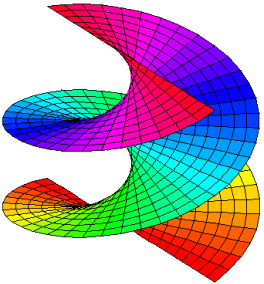
\includegraphics[scale=0.65]{picture/week7/helicoid.png}
        \caption{Helicoid}
    \end{subfigure}
    \begin{subfigure}{0.3\textwidth}
        \centering
        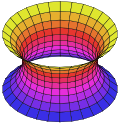
\includegraphics[scale=1.49]{picture/week7/catenoid.png}
        \caption{Catenoid}    
    \end{subfigure}
\end{figure}
\begin{enumerate}[(1)]
    \item Compute the \engordnumber{1} fundamental form of them.
    \[ I_H=\left(v^2+a^2\right)\dd u^2+\dd v^2\]
    \[I_C=\left(a^2\cosh^2\theta\right)\dd\varphi^2+
    \left(a^2\cosh^2\theta\right)\dd \theta^2\]
    \item Show that there is a parametrization on the helicoid, 
    \(\tilde{H}\left(\tilde{u},\tilde{v}\right)\), such that
    \[
        I_{\tilde{H}}=\left(a^2\cosh^2\tilde{v}\right)\dd \tilde{u}^2
        +\left(a^2\cosh^2\tilde{v}^2\right)\dd \tilde{v}^2    
    .\]
    (\(u=\tilde{u},v=a\sinh\tilde{v}\))
\end{enumerate}
\end{example}
\begin{remark}
    In both example 1 and example 3, we have seen that near a point, 
    the two surfaces considered have the same \engordnumber{1} 
    fundamental form
     (after a change of parametrization). Such property is called
      ``local isometry''. We'll make this definition more clear later.
\end{remark}

\(\bullet\)Application of the \engordnumber{1} fundamental form

\begin{enumerate}[(1)]
    \item Arclength of a curve on \(S\).
    
    Note that for a vector \(v\in \mathbb{R}^2\), \(I(v,v)=|v|^2\).
    Let \(\alpha(t)\colon (0,t)\to S\) be a curve in \(S\) and 
    \(\varphi \colon U\to S\), \((u,v)\mapsto\varphi (u,v)\) be a 
    local parametrization satisfying 
    \(\alpha(t)\in \varphi(U)\).
    \[
    \Rightarrow \alpha(t)=\varphi\left(u(t),v(t)\right) .   
    \]
    \[
      \Rightarrow\alpha'(t)=\varphi_u u'(t)+\varphi_v v'(t) .
    \]
    \[\Rightarrow \left|\alpha'(t)\right|^2=
    I\left(\alpha'(t),\alpha'(t)\right)=E u_t^2+2F u_t v_t +G v_t^2.\]
    The arclength of \(\alpha(t)\) is defined by 
    \[
        s(t)=\int_0^t  \left|\alpha'(t)\right|\dd t
        =\int_0^t \sqrt{E u_t^2+2F u_t v_t +G v_t^2}\dd t  .
    \]
    \[
        \Rightarrow \dd s=\sqrt{E u_t^2+2F u_t v_t +G v_t^2}\dd t.
    \]
    \[
        \Rightarrow\left(\dv{s}{t}\right)^2=E u_t^2+2F u_t v_t +G v_t^2.
    \]
    \[
        \Rightarrow \dd s^2=E \dd u^2+2F \dd u \dd v +G \dd v^2    .
    \]
    This explains the ``geometric meaning'' of \(I\), \ie\ it measures 
    the infinitesimal arclength.
    \item Angle between two curves intersecting at \(t_0\).
    
    Let \(\alpha\colon I\to S\), \(\beta\colon I\to S\) be two curves 
    on \(S\), \(\alpha(t_0)=\beta(\bar{t}_0)=p\in S\). 
    \begin{center}
        


\tikzset{every picture/.style={line width=0.75pt}} %set default line width to 0.75pt        

\begin{tikzpicture}[x=0.75pt,y=0.75pt,yscale=-1,xscale=1]
%uncomment if require: \path (0,300); %set diagram left start at 0, and has height of 300

%Curve Lines [id:da9909335153566519] 
\draw    (183,147) .. controls (223,117) and
 (315.4,135.5) .. (363.4,106.5) ;
%Curve Lines [id:da019275275220669075] 
\draw    (167.4,266.5) .. controls (203.4,209.5) and
 (166.4,189.5) .. (183,147) ;
%Curve Lines [id:da6995475257546488] 
\draw    (167.4,266.5) .. controls (207.4,236.5)
 and (299.8,255) .. (347.8,226) ;
%Curve Lines [id:da33316817877336646] 
\draw    (347.8,226) .. controls (383.8,169) and 
(346.8,149) .. (363.4,106.5) ;
%Shape: Circle [id:dp7349369009552857] 
\draw  [fill={rgb, 255:red, 0; green, 0; blue, 0 }  ,fill opacity=1 ] 
(264,167.7) .. controls (264,166.21) and (265.21,165) .. (266.7,165) 
.. controls (268.19,165) and (269.4,166.21) .. (269.4,167.7) .. 
controls (269.4,169.19) and (268.19,170.4) .. (266.7,170.4) .. 
controls (265.21,170.4) and (264,169.19) .. (264,167.7) -- cycle ;
%Curve Lines [id:da09382061994840107] 
\draw    (218,185) .. controls (258,155) and (312.4,171.5) .. (318,185) ;
%Curve Lines [id:da6577705388758515] 
\draw    (245,220) .. controls (258.4,175.5) and (262.4,165.5) .. (302.4,135.5) ;
%Straight Lines [id:da2459893691777446] 
\draw    (266.7,167.7) -- (287.15,142.06) ;
\draw [shift={(288.4,140.5)}, rotate = 128.58] [color={rgb, 255:red, 0; green, 0; blue, 0 }  ]
[line width=0.75]    (10.93,-3.29) .. controls (6.95,-1.4) and (3.31,-0.3) .. (0,0) .. controls 
(3.31,0.3) and (6.95,1.4) .. (10.93,3.29)   ;
%Straight Lines [id:da2821040919294362] 
\draw    (266.7,167.7) -- (304.4,167.51) ;
\draw [shift={(306.4,167.5)}, rotate = 179.71] [color={rgb, 255:red, 0; green, 0; blue, 0 }  ]
[line width=0.75]    (10.93,-3.29) .. controls (6.95,-1.4) and (3.31,-0.3) .. (0,0)
 .. controls (3.31,0.3) 
and (6.95,1.4) .. (10.93,3.29)   ;

% Text Node
\draw (376,118.4) node [anchor=north west][inner sep=0.75pt]    {$S$};
% Text Node
\draw (285,183.4) node [anchor=north west][inner sep=0.75pt]    {$p$};


\end{tikzpicture}
    \end{center}
    Define
        \[
            \cos \theta=\frac{\left\langle\alpha'(t_0),
            \beta'(\bar{t}_0)\right\rangle_{\mathbb{R}^3}}{
            \left|\alpha'(t_0)\right|\left|\beta'(\bar{t}_0) \right|}.
        \]
    \begin{question}
        Given a parametrization \(\varphi(u,v)\),
         we have two coordinate
         curve \(\varphi(u,v_0)\), \(\varphi(u_0,v)\). What's the angle 
         between them?
         \[u\text{-curve: }\alpha(t)=\varphi\left(u(t),c\right)
         \Rightarrow \alpha'(t)=\varphi_u u'.\]
         \[v\text{-curve: }\beta(t)=\varphi\left(c,v(t)\right)
         \Rightarrow \beta'(t)=\varphi_v v'.\] 
         \[
            \Rightarrow \cos \theta= 
            \frac{\left\langle \varphi_u u',\varphi_v v'\right\rangle}{
                \left|\varphi_u u'\right|\left|\varphi_v v'\right|
            }
            =\pm \frac{\left\langle\varphi_u,\varphi_v
            \right\rangle_{\mathbb{R}^3}}{\left|\varphi_u\right|
            \left|\varphi_v\right|}=\pm \frac{F}{\sqrt{EG}}  
         .\]
         In particular, we conclude that
         \[F=0\Leftrightarrow \text{Two coordinate curves are orthogonal,}\]
         and such parametrization is called an orthogonal parametrization.
         (e.g. For \(\mathbb{S}^2\), \((\theta,\varphi)\) and 
         the stereographic projection are two such parametrizations) 
    \end{question}
    \item (Surface) Area.
    
    Let \(S\) be a regular surface. Choose a parametrization 
    \(\varphi\colon U\to S\). Let \(Q\subset S\) be a bounded domain.
    Assume \(Q\subset \varphi(U)\), so \(\varphi^{-1}(Q)\subset U\) is 
    a bounded set in \(\mathbb{R}^2\).
    \begin{center}
\tikzset{every picture/.style={line width=0.75pt}} %set default line width to 0.75pt        

\begin{tikzpicture}[x=0.75pt,y=0.75pt,yscale=-0.9,xscale=0.9]
%uncomment if require: \path (0,300); %set diagram left start at 0, and has height of 300

%Shape: Axis 2D [id:dp30826843172023066] 
\draw  (67,239.62) -- (316.4,239.62)(91.94,114.71) -- (91.94,253.5) (309.4,234.62) -- (316.4,239.62)
 -- (309.4,244.62) (86.94,121.71) -- (91.94,114.71) -- (96.94,121.71)  ;
%Curve Lines [id:da2230443220096674] 
\draw [color={rgb, 255:red, 117; green, 182; blue, 28 }  ,draw opacity=1 ][line width=0.75] 
[line join = round][line cap = round]   (130.65,118.95) .. controls (122.05,125.38) and (127.75,136.1)
.. (124.46,145.32) .. controls (121.04,154.89) and (117.73,154.56) .. (120.74,170.31) .. controls (120.84,170.81) and (138.01,189.7) .. (138.08,189.74) .. controls (142.04,191.95) and (146.26,190.76) .. (150.46,193.9) .. controls (160.22,201.19) and (173.4,214.78) .. (187.61,216.11) .. controls (195.84,216.88) and (204.18,217.17) .. (212.38,216.11) .. controls (218.48,215.32) and (224.1,206.79) .. (229.72,206.39) .. controls (245.72,205.27) and (246.88,208.43) .. (261.91,203.62) .. controls (267,201.99) and (294.17,175.43) .. (297.82,170.31) .. controls (304.87,160.44) and (304.12,147.39) .. (294.11,141.16) .. controls (287.42,136.99) and (273.12,139.67) .. (265.63,138.38) .. controls (261.37,137.65) and (257.55,134.47) .. (253.25,134.22) .. controls (234.05,133.09) and (224.32,137.27) .. (208.67,124.5) .. controls (200.24,117.64) and (182.83,100.69) .. (170.28,99.52) .. controls (154.41,98.04) and (144.45,118.95) .. (130.65,118.95) -- cycle ;
%Curve Lines [id:da779384228982472] 
\draw [line width=0.75] [line join = round][line cap = round]   (176.47,157.04) .. controls (176.47,176.42) and (173.86,179.1) .. (182.66,188.96) .. controls (197.74,205.87) and (228.15,203.16) .. (232.19,173.69) .. controls (232.75,169.62) and (233.14,148.55) .. (228.48,145.93) .. controls (215.25,138.52) and (195.8,139.26) .. (183.9,145.93) .. controls (182.79,146.56) and (180.82,144.74) .. (180.18,145.93) .. controls (179.12,147.92) and (180.91,150.71) .. (180.18,152.87) .. controls (179.34,155.4) and (176.47,157.12) .. (176.47,159.81) ;
%Curve Lines [id:da4093176006038537] 
\draw    (417,115) .. controls (457,85) and (582.4,136.5) .. (622.4,106.5) ;
%Curve Lines [id:da8843839986108935] 
\draw    (421,225) .. controls (461,195) and (586.4,246.5) .. (626.4,216.5) ;
%Curve Lines [id:da3854765584435005] 
\draw    (421,225) .. controls (461,195) and (419.4,153.5) .. (417,115) ;
%Curve Lines [id:da6146348531460317] 
\draw    (626.4,216.5) .. controls (666.4,186.5) and (624.8,145) .. (622.4,106.5) ;
%Curve Lines [id:da8543149552748068] 
\draw [color={rgb, 255:red, 117; green, 182; blue, 28 }  ,draw opacity=1 ][line width=0.75] [line join = round][line cap = round]   (528.4,139.5) .. controls (528.4,138.5) and (528.85,137.39) .. (528.4,136.5) .. controls (527.93,135.57) and (522.09,134.61) .. (521.4,134.5) .. controls (514.38,133.33) and (508.52,128.69) .. (501.4,127.5) .. controls (497.78,126.9) and (494.02,126.9) .. (490.4,127.5) .. controls (488.74,127.78) and (482.76,137.32) .. (482.4,139.5) .. controls (480.99,147.95) and (484.21,151.37) .. (483.4,159.5) .. controls (483,163.53) and (479.56,167.46) .. (479.4,171.5) .. controls (479.09,179.49) and (478.76,187.53) .. (479.4,195.5) .. controls (479.46,196.24) and (481.07,195.83) .. (481.4,196.5) .. controls (489.58,212.86) and (497.61,209.87) .. (513.4,212.5) .. controls (535.53,216.19) and (535.97,204.88) .. (555.4,201.5) .. controls (574.04,198.26) and (600.67,197.05) .. (607.4,173.5) .. controls (611.7,158.44) and (599.25,151.66) .. (589.4,145.5) .. controls (588.77,145.1) and (589.14,143.54) .. (588.4,143.5) .. controls (576.42,142.85) and (564.38,144.11) .. (552.4,143.5) .. controls (548.93,143.32) and (537.92,140.4) .. (533.4,139.5) .. controls (532.08,139.24) and (530.49,135.5) .. (527.4,135.5) ;
%Curve Lines [id:da5437419917187927] 
\draw [line width=0.75] [line join = round][line cap = round]   (524.4,162.5) .. controls (533.93,172.03) and (540,194.41) .. (559.4,186.5) .. controls (570.03,182.17) and (572.69,176.55) .. (575.4,167.5) .. controls (575.66,166.65) and (577.6,162.7) .. (577.4,162.5) .. controls (570.13,155.23) and (537.95,150.97) .. (528.4,151.5) .. controls (524.33,151.73) and (524.4,160.76) .. (524.4,163.5) ;
%Curve Lines [id:da9563040601689965] 
\draw    (318,163) .. controls (358.57,152.71) and (390.12,157.31) .. (416.4,162.67) ;
\draw [shift={(418,163)}, rotate = 191.68] [color={rgb, 255:red, 0; green, 0; blue, 0 }  ][line width=0.75]    (10.93,-3.29) .. controls (6.95,-1.4) and (3.31,-0.3) .. (0,0) .. controls (3.31,0.3) and (6.95,1.4) .. (10.93,3.29)   ;

% Text Node
\draw (178.47,160.44) node [anchor=north west][inner sep=0.75pt]    {$\varphi ^{-1}( Q)$};
% Text Node
\draw (233,106.4) node [anchor=north west][inner sep=0.75pt]    {$U$};
% Text Node
\draw (540,159.4) node [anchor=north west][inner sep=0.75pt]    {$Q$};
% Text Node
\draw (444,140.4) node [anchor=north west][inner sep=0.75pt]    {$\varphi ( U)$};
% Text Node
\draw (661,134.4) node [anchor=north west][inner sep=0.75pt]    {$S$};
% Text Node
\draw (362,133.4) node [anchor=north west][inner sep=0.75pt]    {$\varphi $};
% Text Node
\draw (324,229.4) node [anchor=north west][inner sep=0.75pt]    {$u$};
% Text Node
\draw (85,89.4) node [anchor=north west][inner sep=0.75pt]    {$v$};


\end{tikzpicture}
    \end{center}
    Let's assume the boundary of \(Q\) is a differentiable curve with 
    singularities lying in a measure zero set.
\begin{definition}[Area of \(Q\)]
    \[Area(Q)=\iint_{\varphi(Q)} \left|\varphi_u\wedge 
    \varphi_v \right|\dd u\dd v \quad(\text{double integral in }
    \mathbb{R}^2).\]
    Here, we give the definition in terms of a ``parametrization''. 
    However, the area of \(Q\) is a number only depending on \(Q\)
    itself. We should check that our definition does not depend on 
    the parametrization.
\end{definition}
\textbf{Claim}: 
\textcolor{blue}{\(Area(Q)\) defined above is independent of the
choice of parametrizations.}
\begin{proof} (Left as exercise)

    Let \(\psi(\alpha,\beta)\colon V\to S\) be another parametrization. 
    Let \(H=\psi^{-1}\circ \varphi\) be the change of parametrization,
    \(H(u,v)=(\alpha,\beta)\)\(\Rightarrow\varphi =\psi \circ H\).
    We compute \(\iint_{\varphi(Q)} \left|\varphi_u\wedge 
    \varphi_v \right|\dd u\dd v\).

    By chain rule 
    \[
        \begin{pmatrix}
            \varphi_u\\ \varphi_v
        \end{pmatrix}=
        \pdv{(\alpha,\beta)}{(u,v)}\begin{pmatrix}
            \psi_\alpha\\
            \psi_\beta
        \end{pmatrix}    .
    \]
    \begin{align*}
        \Rightarrow \varphi_u\wedge\varphi_v&=
        \left(\alpha_u\beta_v\right)\psi_\alpha\wedge\psi_\beta+
        \left(\alpha_v\beta_u\right)\psi_\beta\wedge\psi_\alpha\\
        &=\left(\alpha_u\beta_v-\alpha_v\beta_u\right)
        \psi_\alpha\wedge\psi_\beta\\
        &=\det\left(\pdv{(\alpha,\beta)}{(u,v)}\right)
        \psi_\alpha\wedge\psi_\beta.
    \end{align*}
    \[\Rightarrow \left|
        \varphi_u\wedge \varphi_v 
    \right|=\left|\det\left(\pdv{(\alpha,\beta)}{(u,v)}\right)\right|
    \left|\psi_\alpha\wedge\psi_\beta\right|.\]
    
    On the other hand,
    \[
        \begin{pmatrix}
            \dd u\\ \dd v
        \end{pmatrix}
        =\pdv{(u,v)}{(\alpha,\beta)}\begin{pmatrix}
            \dd \alpha\\
            \dd \beta
        \end{pmatrix} .
    \]
    Thus, the change of infinitesimal area element is
    \[
        \dd u\dd v=\left|\dd u\wedge\dd v\right|=
        \left|\det \left(\pdv{(u,v)}{(\alpha,\beta)}\right)\right|
        \left|\dd\alpha\wedge\dd\beta\right|=
        \left|\det \left(\pdv{(u,v)}{(\alpha,\beta)}\right)\right|
        \dd\alpha\dd\beta.
    \]
    \[\Rightarrow \left|\varphi_u\wedge \varphi_v \right|
        \dd u\dd v=\left|\psi_\alpha\wedge\psi_\beta\right|\dd \alpha
        \dd \beta.
    \]
    \[\Rightarrow \iint \left|\varphi_u\wedge \varphi_v \right|
    \dd u\dd v=\iint \left|\psi_\alpha\wedge\psi_\beta\right|\dd \alpha
    \dd \beta.\]
\end{proof}
\begin{remark}
    By the \engordnumber{1} fundamental form 
    \[
        I=E(\dd u)^2+2F \dd u\dd v+G(\dd v)^2    
    \]
    \[\Rightarrow Area=\iint \left|\varphi_u\wedge \varphi_v \right|
    \dd u\dd v=\iint \sqrt{EG-F^2}\dd u\dd v.\]
\end{remark}
\end{enumerate}
\section{Gauss maps and the \texorpdfstring{\engordnumber{2}}{2nd} fundamental form}
\(\bullet\) Gauss maps.
\begin{question}
    \textcolor{blue}{How is a regular surface curved in \(\mathbb{R}^3\)}? 
\end{question}
\underline{\textbf{Recall}}: \(S\subset\mathbb{R}^3\) is an oriented
regular surface. 
\(\Rightarrow\) We can choose a unit vector field 
    \begin{align*}
        \vb{n}\colon S&\to \mathbb{S}^2(1)\\
        p&\mapsto \vb{n}_p,
    \end{align*}
is well-defined everywhere on \(S\). Moreover, \(\vb{n}\) is a
differentiable map with its image lying on the unit sphere, and we 
called the map to be the Gauss map. \(\vb{n}\) determines an 
orientation of \(S\).
\begin{center}
    


\tikzset{every picture/.style={line width=0.75pt}} %set default line width to 0.75pt        

\begin{tikzpicture}[x=0.75pt,y=0.75pt,yscale=-1,xscale=1]
%uncomment if require: \path (0,300); %set diagram left start at 0, and has height of 300

%Curve Lines [id:da28129415507356703] 
\draw    (100,110) .. controls (140,80) and (233.8,125) .. (267.4,89.5) ;
%Curve Lines [id:da9562883564686324] 
\draw    (59,172) .. controls (99,142) and (192.8,187) .. (226.4,151.5) ;
%Curve Lines [id:da748577885122705] 
\draw    (59,172) .. controls (72.4,131.5) and (99.4,129.5) .. (100,110) ;
%Curve Lines [id:da2562375766370064] 
\draw    (226.4,151.5) .. controls (217.4,127.5) and (250.4,106.5) .. (267.4,89.5) ;
%Shape: Parallelogram [id:dp8965230202175429] 
\draw   (145.82,117.5) -- (201.4,117.5) -- (177.58,145.5) -- (122,145.5) -- cycle ;
%Shape: Circle [id:dp3509817579048975] 
\draw  [fill={rgb, 255:red, 0; green, 0; blue, 0 }  ,fill opacity=1 ] (161.7,131.5) .. controls (161.7,130.01) and (162.91,128.8) .. (164.4,128.8) .. controls (165.89,128.8) and (167.1,130.01) .. (167.1,131.5) .. controls (167.1,132.99) and (165.89,134.2) .. (164.4,134.2) .. controls (162.91,134.2) and (161.7,132.99) .. (161.7,131.5) -- cycle ;
%Straight Lines [id:da4477857542457926] 
\draw    (164.4,131.5) -- (163.44,81.5) ;
\draw [shift={(163.4,79.5)}, rotate = 88.9] [color={rgb, 255:red, 0; green, 0; blue, 0 }  ][line width=0.75]    (10.93,-3.29) .. controls (6.95,-1.4) and (3.31,-0.3) .. (0,0) .. controls (3.31,0.3) and (6.95,1.4) .. (10.93,3.29)   ;
%Shape: Axis 2D [id:dp2767501351977306] 
\draw  (465,150) -- (565,150)(475,60) -- (475,160) (558,145) -- (565,150) -- (558,155) (470,67) -- (475,60) -- (480,67)  ;
%Straight Lines [id:da9011328855757925] 
\draw    (475,150) -- (407.83,216.1) ;
\draw [shift={(406.4,217.5)}, rotate = 315.46] [color={rgb, 255:red, 0; green, 0; blue, 0 }  ][line width=0.75]    (10.93,-3.29) .. controls (6.95,-1.4) and (3.31,-0.3) .. (0,0) .. controls (3.31,0.3) and (6.95,1.4) .. (10.93,3.29)   ;
%Shape: Circle [id:dp28714049477405257] 
\draw  [color={rgb, 255:red, 144; green, 19; blue, 254 }  ,draw opacity=1 ] (431.8,150) .. controls (431.8,126.14) and (451.14,106.8) .. (475,106.8) .. controls (498.86,106.8) and (518.2,126.14) .. (518.2,150) .. controls (518.2,173.86) and (498.86,193.2) .. (475,193.2) .. controls (451.14,193.2) and (431.8,173.86) .. (431.8,150) -- cycle ;
%Straight Lines [id:da45439583119974114] 
\draw    (475,150) -- (439.08,126.59) ;
\draw [shift={(437.4,125.5)}, rotate = 33.09] [color={rgb, 255:red, 0; green, 0; blue, 0 }  ][line width=0.75]    (10.93,-3.29) .. controls (6.95,-1.4) and (3.31,-0.3) .. (0,0) .. controls (3.31,0.3) and (6.95,1.4) .. (10.93,3.29)   ;
%Curve Lines [id:da1330380081969107] 
\draw    (283,139) .. controls (322.4,109.45) and (349.58,123.08) .. (381.54,138.3) ;
\draw [shift={(383,139)}, rotate = 205.43] [color={rgb, 255:red, 0; green, 0; blue, 0 }  ][line width=0.75]    (10.93,-3.29) .. controls (6.95,-1.4) and (3.31,-0.3) .. (0,0) .. controls (3.31,0.3) and (6.95,1.4) .. (10.93,3.29)   ;

% Text Node
\draw (190,136.4) node [anchor=north west][inner sep=0.75pt]    {$T_{p} S$};
% Text Node
\draw (158,56.4) node [anchor=north west][inner sep=0.75pt]    {$\vb{n}$};
% Text Node
\draw (147.82,120.9) node [anchor=north west][inner sep=0.75pt]    {$p$};
% Text Node
\draw (262,70.4) node [anchor=north west][inner sep=0.75pt]    {$S$};
% Text Node
\draw (390,214.4) node [anchor=north west][inner sep=0.75pt]    {$x$};
% Text Node
\draw (577,141.4) node [anchor=north west][inner sep=0.75pt]    {$y$};
% Text Node
\draw (469,38.4) node [anchor=north west][inner sep=0.75pt]    {$z$};
% Text Node
\draw (517,93.4) node [anchor=north west][inner sep=0.75pt]    {$\mathbb{S}^{2}$};
% Text Node
\draw (418,102.4) node [anchor=north west][inner sep=0.75pt]   {$\vb{n}_{p}$};
% Text Node
\draw (326,98.4) node [anchor=north west][inner sep=0.75pt]    {$\vb{n}$};


\end{tikzpicture}
\end{center}
Let \(\varphi \colon U\to S\) be a local parametrization near 
\(p\in S\), then 
\[
    \vb{n}=\frac{\varphi_u\wedge\varphi_v}{
        \left|\varphi_u\wedge\varphi_v\right|}.    
\]
Let's compute the differential of the Gauss map at \(p\).
\[
    \dd\vb{n}_p\colon T_p S\to T_{\vb{n}_p}\mathbb{S}^2    .
\]
\(\forall v\in T_p S\), let \(\alpha(s)\) be the curve on \(S\)
such that \(\alpha(0)=p\), \(\alpha'(0)=v\).
\[
    \Rightarrow
    \dd\vb{n}_p(v)=\left.\dv{s}\right|_{s=0}\vb{n}\left(\alpha(s)\right)
    (\text{changing rate of the Gauss map at }p
    \text{ along direction }v).
\]
Note \(\left\langle\vb{n}\left(\alpha(s)\right),
\vb{n}\left(\alpha(s)\right)\right\rangle=1\), taking derivation at 
\(s=0\): 
\[
\left\langle\left.\dv{s}\right|_{s=0}\vb{n}\left(\alpha(s)\right),
\vb{n}_p \right\rangle=0.
\]
\[
    \Rightarrow 
    \dd\vb{n}_p(v)=\left.\dv{s}\right|_{s=0}\vb{n}\left(\alpha(s)\right)
    \in T_p S.
\]
\begin{definition}[The \engordnumber{2} fundamental form]
    \hfill
    \begin{itemize}
        \item \(\forall v\in T_p S\), the \engordnumber{2} fundamental
        form 
        \[\II_p(v,v)=
        -\left\langle \dd\vb{n}_p(v),
        v\right\rangle_{\mathbb{R}^3}\footnotemark.\]
        \footnotetext{Thus, \(\dd\vb{n}_p\colon T_p S\to T_p S\) 
        is a linear map, which is the directional derivation of 
        \(\vb{n}\) along a tangent direction of \(S\).}
        \item More generally \(\forall v,w\in T_p S\), 
        \[
            \II_p\colon T_p S\times T_p S\to T_p \mathbb{R}
        \]
         \[   (v,w)\mapsto \II_p(v,w)=-\left\langle
                \dd\vb{n}_p(v),w\right\rangle_{\mathbb{R}^3}.
        \]

    \end{itemize}
    \(-\dd \vb{n}_p\) is also called the shape operator.
\end{definition}
Before we explore \(\II_p\), let's compute the Gauss map's
differential.

\(\bullet\) Let \(\varphi(u,v)\) be a local parametrization. 
Any curve on \(S\) has parametrization
\[  
    \alpha(t)=\varphi\left(u(t),v(t)\right)=
    \left(x\left(u(t),v(t)\right),
        y\left(u(t),v(t)\right),
        z\left(u(t),v(t)\right)\right).
\]
\[\Rightarrow \alpha'(0)=\varphi_u u'(0)+\varphi_v v'(0).\]
\begin{align*}
    \dd \vb{n}_p\left(\alpha'(0)\right)
    &=\left.\dv{t}\right|_{t=0}\vb{n}\left(\alpha(t)\right)\\
    &=\left.\dv{t}\right|_{t=0}\vb{n}
    \left(x\left(u(t),v(t)\right),
        y\left(u(t),v(t)\right),
        z\left(u(t),v(t)\right)\right)\\
    &=\left(\vb{n}_x x_u+\vb{n}_y y_u+\vb{n}_z z_u\right)u'(0)
    +\left(\vb{n}_x x_v+\vb{n}_y y_v+\vb{n}_z z_v\right)v'(0)\\    
    &=\vb{n}_u u'(0)+\vb{n}_v v'(0).
\end{align*}
On the other hand, by the linearity of \(\dd \vb{n}_p\), 
\[
    \dd\vb{n}_p\left(\alpha'(0)\right)=u'(0)\dd \vb{n}_p
    \left(\varphi_u\right)+v'(0)\dd\vb{n}_p \left(\varphi_v\right).    
\]
\[
    \Rightarrow
    \begin{cases}
        \dd\vb{n}_p\left(\vphi_u\right)=\vb{n}_u,\\
        \dd\vb{n}_p\left(\vphi_v\right)=\vb{n}_v.
    \end{cases}
\]
\begin{align*}
    \left\langle \dd\vb{n}_p\left(\vphi_u\right),\vphi_u
    \right\rangle
    &=\left\langle\vb{n}_u,\vphi_u\right\rangle=
    \pdv{u}\underbrace{\left\langle\vb{n},\vphi_u\right\rangle}_{=0}
    -\left\langle\vb{n},\vphi_{uu}\right\rangle\\
    \left\langle \dd\vb{n}_p\left(\vphi_u\right),\vphi_v
    \right\rangle
    &=\left\langle\vb{n}_u,\vphi_v\right\rangle\\
    &=\pdv{u}\underbrace{\left\langle\vb{n},\vphi_v\right\rangle}_{=0}
    -\left\langle\vb{n},\vphi_{vu}\right\rangle\\
    &=-\left\langle\vb{n},\vphi_{vu}\right\rangle\\
    \left\langle \dd\vb{n}_p\left(\vphi_v\right),\vphi_u
    \right\rangle
    &=\left\langle\vb{n}_v,\vphi_u\right\rangle\\
    &=-\left\langle\vb{n},\vphi_{uv}\right\rangle
    (\text{Note that }\vphi_{uv}=\vphi_{vu}\text{ since }
    \vphi\text{ is smooth})\\
    \left\langle \dd\vb{n}_p\left(\vphi_v\right),\vphi_v
    \right\rangle
    &=\left\langle\vb{n}_v,\vphi_v\right\rangle
    =-\left\langle \vb{n}, \vphi_{vv}\right\rangle.
\end{align*}
Hence, we conclude that: 
\begin{theorem}
    \(\II_p(v,w)=\II_p(w,v)\), \ie\ 
    \(\II_p\) is symmetric in \(v\), \(w\), and
    \(\II_p\) is a bilinear form. 
\end{theorem}
\begin{remark}
    \hfill
    \begin{enumerate}[(1)]
        \item From the computation above, we see that 
        \(\dd\vb{n}_p\) is self-adjoint, \ie\ 
        \(\left\langle \dd\vb{n}_p(v),w\right\rangle=
        \left\langle v, \dd\vb{n}_p(w)\right\rangle
        \).
        \item The \engordnumber{2} fundamental form can be also 
        defined as 
        \[\II_p(v,v)=\left\langle\vb{n}_p,\alpha''(0)\right\rangle,\]
        where \(\alpha\) is a curve with \(\alpha'(0)=v\).
    \end{enumerate}
\end{remark}
\begin{exercise}
    Check that this definition coincides with the previous one.
\end{exercise}
\begin{proof}
    Along the curve \(\alpha(t)\in S\), \(\left\langle
    \vb{n}\left(\alpha(t)\right),\alpha'(t)\right\rangle=0\).
    Therefore, 
    \begin{align*}
        0&=\dv{t}\left\langle\vb{n}\left(\alpha(t)\right),\alpha'(t)
        \right\rangle\\
        &= \left\langle \dd\vb{n}_{\alpha(t)}\left(\alpha'(t)
        ,\alpha'(t)\right)\right\rangle+\left\langle
         \vb{n}\left(\alpha(t)\right),\alpha''(t)\right\rangle.
    \end{align*}
\end{proof}
Just as the \engordnumber{1} fundamental form, we write \(\II\) as 
\[
    \II_p=e\dd u^2+2f\dd u\dd v+g\dd v^2,
\]
where 
\begin{align*}
    e&=-\left\langle \dd\vb{n}_p\left(\varphi_u\right),\varphi_u\right\rangle
    =-\left\langle\vb{n}_u,\varphi_u\right\rangle=\left\langle
        \vb{n},\varphi_{uu}\right\rangle\\
    f&=-\left\langle \dd\vb{n}_p\left(\varphi_u\right),\varphi_v\right\rangle
    =-\left\langle\vb{n}_u,\varphi_v\right\rangle=\left\langle
        \vb{n},\varphi_{uv}\right\rangle\\
        (&=-\left\langle \dd\vb{n}_p\left(\varphi_v\right),\varphi_u
        \right\rangle=-\left\langle\vb{n}_v,\varphi_u\right\rangle
        =\left\langle\vb{n},\varphi_{vu}\right\rangle)\\
        g&=-\left\langle \dd\vb{n}_p\left(\varphi_v\right),\varphi_v
        \right\rangle=-\left\langle\vb{n}_v,\varphi_v
        \right\rangle=\left\langle\vb{n},\varphi_{vv}\right\rangle
\end{align*}
\(\bullet\) Weingarten equations (linear representation of \(\dd\vb{n}\)
in \(\{\varphi_u,\varphi_v\}\))

We have seen \(\dd{\vb{n}}_p\colon T_p S\to T_{\vb{n}_p}\mathbb{S}^2\)
has image actually lying in \(T_p S=\Span\left\{\varphi_u,
\varphi_v\right\}\) in terms of a local parametrization \(\varphi(u,v)\).
\[
    \Rightarrow \begin{cases}
        \dd\vb{n}_p\left(\varphi_u\right)=a_{11}\varphi_u+a_{12}\varphi_v\\
        \dd\vb{n}_p\left(\varphi_v\right)=a_{21}\varphi_u+a_{22}\varphi_v
    \end{cases}
    \ie\ \begin{cases}
        \vb{n}_u=a_{11}\varphi_u+a_{12}\varphi_v\\
        \vb{n}_v=a_{21}\varphi_u+a_{22}\varphi_v
    \end{cases}
\]
We would like to find out the matrix \(\begin{pmatrix}
    a_{11}&a_{12}\\
    a_{21}&a_{22}
\end{pmatrix}\).

Recall that 
\[
    I_p=E\dd u^2+2F \dd u\dd v+G\dd v^2,
\]
where
\[
    E=\left\langle\varphi_u,\varphi_u\right\rangle,
    F=\left\langle\varphi_u,\varphi_v\right\rangle,
    G=\left\langle\varphi_v,\varphi_v\right\rangle.    
\]
Now we consider the matrix 
\[
    \begin{pmatrix}
        \vb{n}_u\\
        \vb{n}_v
    \end{pmatrix}
    \begin{pmatrix}
        \varphi_u &\varphi_v
    \end{pmatrix}=
    \begin{pmatrix}
        \left\langle\vb{n}_u,\varphi_u\right\rangle&
        \left\langle\vb{n}_u,\varphi_v\right\rangle\\
        \left\langle\vb{n}_v,\varphi_u\right\rangle&
        \left\langle\vb{n}_v,\varphi_v\right\rangle
    \end{pmatrix}.    
\]
On the one hand, the R.H.S. is 
\[
    \begin{pmatrix}
    -e&-f\\
    -f&-g
    \end{pmatrix}=-
    \begin{pmatrix}
        e&f\\
        f&g
    \end{pmatrix}.
\]
On the other hand,
\begin{align*}
    \text{R.H.S.}&=\begin{pmatrix}
        a_{11}E+a_{12}F&
        a_{11}F+a_{12}G\\
        a_{21}E+a_{22}F&
        a_{21}F+a_{22}G
    \end{pmatrix}\\
    &=\begin{pmatrix}
        a_{11}&a_{12}\\
        a_{21}&a_{22}
    \end{pmatrix}
    \begin{pmatrix}
        E&F\\
        F&G
    \end{pmatrix}.
\end{align*}
\[
    \Rightarrow 
    -\underbrace{\begin{pmatrix}
        e&f\\
        f&g
    \end{pmatrix}}_{\II}
    =
    \begin{pmatrix}
        a_{11}&a_{12}\\
        a_{21}&a_{22}
    \end{pmatrix}
    \underbrace{\begin{pmatrix}
        E&F\\
        F&G
    \end{pmatrix}}_{I}.
\]
\begin{align*}
    \Rightarrow
    \begin{pmatrix}
        a_{11}&a_{12}\\
        a_{21}&a_{22}
    \end{pmatrix}
    &=-\begin{pmatrix}
        e&f\\
        f&g
    \end{pmatrix}
    \begin{pmatrix}
        E&F\\
        F&G
    \end{pmatrix}^{-1}\\
    &=-\begin{pmatrix}
        e&f\\
        f&g
    \end{pmatrix}
    \frac{1}{\det}\begin{pmatrix}
        G&-F\\
        -F&E
    \end{pmatrix}\\
    &=-\frac{1}{EG-F^2}\begin{pmatrix}
        e&f\\
        f&g
    \end{pmatrix}
    \begin{pmatrix}
        G&-F\\
        -F&E
    \end{pmatrix}\\
    &=\frac{1}{EG-F^2}\begin{pmatrix}
        fF-eG& e F-fE\\
        gF-fG& fF-gE
    \end{pmatrix}\tag{\(\ast \)}.
\end{align*}
The Weingarten equation is \(\dd\vb{n}_p\sim \begin{pmatrix}
    a_{11}&a_{12}\\
    a_{21}&a_{22}
\end{pmatrix}\),
\ie\ 
\[
    \begin{pmatrix}
        \vb{n}_u\\
        \vb{n}_v
    \end{pmatrix}=
    \begin{pmatrix}
        a_{11}&a_{12}\\
        a_{21}&a_{22}
    \end{pmatrix}
    \begin{pmatrix}
        \varphi_u\\
        \varphi_v
    \end{pmatrix},
\]
with \(\begin{pmatrix}
    a_{11}&a_{12}\\
    a_{21}&a_{22}
\end{pmatrix}\) defined in (\(\ast\)).

\begin{itemize}
    \item[{\Large\textcolor{red}{\textbf{!}}}]
    For a regular surface \(S\subset \mathbb{R}^3\), 
    if we know the local parametrization \(\varphi(u,v)\) near 
    a point \(p\), then 
    \[
        I_p=E\dd u^2+2F \dd u\dd v+G\dd v^2,
    \]
    and 
    \[
        \II_p=e\dd u^2+2f\dd u\dd v+g\dd v^2,
    \]
    are fully understood with
    \[
        \begin{pmatrix}
            E&F\\
            F&G
        \end{pmatrix}
        =\begin{pmatrix}
            \left\langle\varphi_u,\varphi_u\right\rangle
            &
            \left\langle\varphi_u,\varphi_v\right\rangle
            \\
            \left\langle\varphi_v,\varphi_u\right\rangle
            &
            \left\langle\varphi_v,\varphi_v\right\rangle
        \end{pmatrix},
    \]
    and 
    \[
        \begin{pmatrix}
            e&f\\
            f&g
        \end{pmatrix}
        =\begin{pmatrix}
            \left\langle\varphi_{uu},\vb{n}\right\rangle&
            \left\langle\varphi_{uv},\vb{n}\right\rangle\\
            \left\langle\varphi_{vu},\vb{n}\right\rangle &
            \left\langle\varphi_{vv},\vb{n}\right\rangle
        \end{pmatrix}.
    \]
\end{itemize}
\begin{example}
    \begin{enumerate}[(1)]
        \hfill
        \item Plane: \(Ax +B y+C z+D=0 \)
        \[\vb{n}=\frac{(A,B,C)}{\sqrt{A^2+B^2+C^2}}\]
        is a constant map. Thus, 
        \(
            \dd\vb{n}=0    
        \) and \(\II(v,v)=-\left\langle \dd\vb{n}(v),v\right\rangle=0\).
        \item \(\mathbb{S}^2(1)=\{x^2+y^2+z^2=1\}\).
        At point \((x,y,z)\), the unit normal vector field is 
        \(\vb{n}_{\pm}=\pm (x,y,z)\), where \(\vb{n}_+\) means 
        the outer normal vector, and \(\vb{n}_-\) the inner normal 
        vector.

        Let's consider \(\vb{n}_-=-(x,y,z)\), let \(\alpha(t)=\left(
        x(t),y(t),z(t)\right)\) be a curve on \(\mathbb{S}^2\), then 
        \[
            \dd\vb{n}_-\left(\alpha'(t)\right)
            =\dv{t}\vb{n}_- \left(\alpha(t)\right)
            =-\dv{t}\left(x(t),y(t),z(t)\right)
            =-\alpha'(t)    
        .\]
        \[\Rightarrow
            \II\left(\alpha'(t),\alpha'(t)\right)
            =-\left\langle \dd\vb{n}_-\left(\alpha'(t)\right)
            \right\rangle=\left\langle\alpha'(t),\alpha'(t)
            \right\rangle=\left|\alpha'(t)\right|^2\ge 0.
        \]
        If we take \(\vb{n}_+\), then 
        \[\II\left(\alpha'(t),\alpha(t)\right)=
        -\left|\alpha'(t)\right|^2\le 0.\]
        \underline{Hence}, sign of the \engordnumber{2} fundamental form
    depends on the choice of orientation (\ie\ the unit normal).
    \item Helicoid (in which every point looks like a saddle point).
    \[H(u,v)=(v\cos u,v\sin u,a u)\]
    \[H_u=(-v\sin u,v\cos u,a),\quad H_v=(\cos u,\sin u,0).\]
    \[H_{uu}=(-v\cos u,-v\sin u,0),H_{uv}=(-\sin u,\cos u,0),
    H_{vv}=(0,0,0).
    \]
    \[
        \vb{n}=\left(-\frac{a\sin u}{\sqrt{a^2+v^2}},
        \frac{a\cos u}{\sqrt{a^2+v^2}},
        -\frac{v}{\sqrt{a^2+v^2}}
        \right).    
    \]
    \[
        \II=\frac{2a}{\sqrt{a^2+v^2}}\dd u\dd v    ,
    \]
    \ie\ 
    \[
        \begin{pmatrix}
            e&f\\
            f&g
        \end{pmatrix}=\begin{pmatrix}
            0&\frac{2a}{\sqrt{a^2+v^2}}\\
            \frac{2a}{\sqrt{a^2+v^2}}&0
        \end{pmatrix},\quad
        \lambda=\pm \frac{a}{\sqrt{a^2+v^2}}\text{ indefinite}.
    \]
    \item Cylinder. \(x^2+y^2=1\)
    \[
        c(\theta,v)=(\cos \theta,\sin\theta,v).    
    \]
    \[
        c_\theta=(-\sin \theta,\cos \theta,0),\quad
        c_v=(0,0,1).    
    \]
    \[
        \vb{n}_+=(\cos\theta,\sin\theta,0)(\text{the outer normal}),    
    \]
    \[
        \vb{n}_-=(-\cos\theta,-\sin\theta,0)(\text{the inner normal}).
    \]
    \[
        c_{\theta\theta}=(-\cos \theta,-\sin\theta,0),\quad
        c_{\theta v}=(0,0,0),\quad
        c_{vv}=(0,0,0).    
    \]
    \[\Rightarrow \II_{\vb{n}_-}=d \theta^2\sim \begin{pmatrix}
        1&0\\0&0
    \end{pmatrix}.\]
    \end{enumerate}  
\end{example}
\begin{remark}
    The cylinder and the plane have the same \engordnumber{1} fundamental
    form, but different \engordnumber{2} fundamental form.
\end{remark}
\section{Geometric meaning of the \texorpdfstring{\engordnumber{2}}{2nd} fundamental form and curvatures}
\underline{Recall}: \begin{itemize}
    \item Gauss map \[\vec{N}\colon S\to \mathbb{S}^2(1),\]
    \[p\mapsto \vec{N}_p.\]
    \item \(d \vec{N}_p\colon T_p S\to T_{\vec{N}(p)}\mathbb{S}^2(1)
    \simeq T_p S\).
    \item \(\forall v \in T_p S\), \(\II(v,v)=-\left\langle d 
    \vec{N}_p(v),v
    \right\rangle=\left\langle \vec{N}_p,
    \alpha''(0)\right\rangle\), where
    \(\alpha\) is a curve with \(\alpha(0)=p\), \(\alpha'(0)=v\).
\end{itemize}
(Note that at \(p\) along direction \(v\), there are indefinitely
many, curves passing through \(p\) with tangent vector \(v\), each
can be obtained by using a plane containing \(p,v\) to intersect with
\(S\)). However, \(\II(v,v)\) only depends on \(\alpha'(0)=v\).

\underline{Goal}: Understanding how \engordnumber{2} fundamental 
form reflects the surface is curved locally near a point.
\subsection{Normal curvature}
    
    Let \(\alpha(s)\) be a regular curve parametrized by the arclength In
    \(S\). 
    \[
        \Rightarrow \alpha'(s)=t(s),\quad \left|\alpha'(s)\right|=1
    \]
    \[
        \alpha''(s)=t'(s)=k(s)\vb{n}(s),\quad k(s):\text{curvature of
        }\alpha(s),\quad\vb{n}:\text{unit normal vector of }\alpha(s)
    \]
\begin{align*}
    \left\langle\alpha''(s),\vec{N}\left(\alpha(s)\right)\right\rangle
    &=\dv{s}\langle\underbrace{\alpha'(s)}_{\in T_{\alpha(s)}S}
    \vec{N}\left(\alpha(s)\right)\rangle-\left\langle
        \alpha'(s),\dv{s}\vec{N}\left(\alpha(s)\right)
    \right\rangle\\
    &=-\left\langle\alpha'(s),d\vec{N}_{\alpha(s)}\left(\alpha'(s)
    \right)\right\rangle\\
    &=\II\left(\alpha'(s),\alpha'(s)\right)
\end{align*}
On the other hand, 
\[
    \left\langle\alpha''(s),\vec{N}(\alpha(s))\right\rangle    
    =\left\langle k(s) \vb{n}(s),\vec{N}(s)\right\rangle
    =k(s)\cos \theta.
\]
This is the projection of ``curvature'' of \(\alpha(s)\) on the normal
vector of the surface. We call the value
\[
    k_{\vb{n}}=k(s)\cos \theta
\]
to be the ``normal curvature of curve \(\alpha(s)\)''.

Hence, the \engordnumber{2} fundamental form
\[
    \II\left(\alpha'(s),\alpha'(s)\right)    
    =\text{normal curvature of }\alpha(s)=k_{\vb{n}}.
\]
But \(\II\left(\alpha'(s),\alpha'(s)\right)\) only depends on 
\(\alpha'(s)\) but not a particular curve. Hence, at \(p\in S\), 
all curves passing through \(p\) with the same unit tangent vector
\(v\) have the same normal curvature. A canonical choice of
such curve is called the ``normal section'' which is a curve 
obtained by intersecting the plane \(\Span\{\underbrace{v}_{unit},N\}\)
with \(S\)
\[
    \Rightarrow k_{\vb{n}}=\pm \text{curvature of normal section along
    direction }v.
\]
\[
    \Rightarrow \II(v,v)= \pm \text{curvature of normal section along
    direction }v.   
\]
\begin{exercise}
    Compute \(k_{\vb{n}}\) in a local parametrization.

    Let \(\alpha(s)=\varphi\left(u(s),v(s)\right)\), 
    \(\alpha'(s)=\varphi_u u'(s)+\varphi_v v'(s)\), where \(s\)
    is the arclength parameter. Then, 
    \[
        \alpha''(s)=\varphi_{uu}\left(u'(s)\right)^2 +2\varphi_{uv}
        u'(s)v'(s)+\varphi_{vv}\left(v'(s)\right)^2
        +\underbrace{\varphi_u u''(s)+\varphi_v v''(s)}_{tangential}.
    \]
    \begin{align*}
        &\left\langle \alpha''(s),
        \vec{N}\left(\alpha(s)\right)\right\rangle\\
        =&\left\langle \varphi_{uu},\vec{N}\right\rangle
        \left(u'(s)\right)^2 +2\left\langle\varphi_{uv},
        \vec{N}\right\rangle u'(s)v'(s)+\left\langle
        \varphi_{vv},\vec{N}\right\rangle\left(v'(s)\right)^2\\
        =&e \left(u'(s)\right)^2+2fu'(s)v'(s)+g\left(v'(s)\right)^2
    .\end{align*}
    Therefore, 
    \[
        k_{\vb{n}}\left(\alpha'(s)\right)=
        e \left(u'(s)\right)^2+2fu'(s)v'(s)+g\left(v'(s)\right)^2.
    \]
    It's also interesting to obtain \(k_{\vb{n}}\) in an 
    arbitrary parametrization. Let \(\alpha(\tau)\) be some parameter,
    \[
        \Rightarrow
        S=\left(\tau\right)    \int_0^\tau \left|\alpha'(\tau)\right|
        \dd \tau
        ,\quad \tau'(s)=\frac{1}{\left|\alpha'(\tau)\right|}.
    \]
    \begin{align*}
        \alpha'(s)&=\alpha'(\tau)\tau'(s),\\
        \alpha''(s)&=\alpha''(\tau)\left(\tau'(s)\right)^2+
        \alpha'(\tau)\tau''(s).
    \end{align*}
    \begin{align*}
        \left\langle\alpha''(s),\vec{N}\left(\alpha(\tau)\right)
        \right\rangle
        &=\left\langle\alpha''(\tau),\vec{N}\left(\alpha(\tau)\right)
        \right\rangle\left(\tau'(s)\right)^2\\
        &=\frac{\II\left(\alpha'(\tau),\alpha'(\tau)\right)}{
            I\left(\alpha'(\tau),\alpha'(\tau)\right)
        }.
    \end{align*}
    \[
        \therefore   k_{\vb{n}}\left(\alpha'(\tau)\right)
        =\frac{\II\left(\alpha'(\tau),\alpha'(\tau)\right)}{
            I\left(\alpha'(\tau),\alpha'(\tau)\right)
        }.
    \]
\end{exercise}
\begin{itemize}
    \item[{\Large\textcolor{red}{\textbf{!}}}] The normal curvature
    along direction \(v\) is \(\II(v,v)\) tells us that how the 
    surface is curved along direction \(v\) at \(p\).
\end{itemize}
\begin{example}\label{normal curvature-sphere}
    Sphere: \(x^2+y^2+z^2=1\).
\end{example}

Normal sections are the great circles of radius \(1\).
         \[\therefore \II(v,v)=1,\quad\forall |v|=1.\]
        \begin{center}
            \begin{tikzpicture}[scale=2]%抄的知乎:https://zhuanlan.zhihu.com/p/494100190
                \pgfmathsetmacro{\R}{2};
                \pgfmathsetmacro{\AngleGamma}{25}
                \tikzset{%>=latex, % option for nice arrows
                    inner sep=0pt,%
                    outer sep=2pt,%
                     mark coordinate/.style=
                     {inner sep=0pt,outer sep=0pt,minimum size=3pt,
                    fill=black,circle}%
                        }
            \newcommand\LongitudePlane[3][current plane]{
            \tikzset{#1/.estyle={cm={cos(#3),sin(#3)*sin(#2),0,cos(#2),(0,0)}}}}
            \newcommand\DrawLongitude[3][\AngleGamma]{
            \LongitudePlane{#1}{#3}
            \tikzset{current plane/.prefix style={scale=#2}}
                             % angle of "visibility"
            \pgfmathsetmacro\angVis{atan(sin(#3)*cos(#1)/sin(#1))} %
            \draw[current plane,thin,black] 
            (\angVis:1) arc (\angVis:\angVis+180:1);
            \draw[current plane,thin,dashed] 
            (\angVis-180:1) arc (\angVis-180:\angVis:1);
            }
            \newcommand\LatitudePlane[3][current plane]{
  \pgfmathsetmacro\yshift{cos(#2)*sin(#3)}
  % 下面 cm 的最后一个参数不能出现乘法,所以定义了 yshift
  \tikzset{#1/.estyle={cm={cos(#3),0,0,cos(#3)*sin(#2),(0,\yshift)}}}
}
% 参数1:【可选】极点的倾斜角,默认 `\AngleGamma`
% 参数2:地球半径
% 参数3:维度(北正南负)
\newcommand\DrawLatitude[3][\AngleGamma]{
  \LatitudePlane{#1}{#3}
  \tikzset{current plane/.prefix style={scale=#2}}
  \pgfmathsetmacro\sinVis{sin(#3)/cos(#3)*sin(#1)/cos(#1)}
  % angle of "visibility"
  \pgfmathsetmacro\angVis{asin(min(1,max(\sinVis,-1)))}
  \draw[current plane,thin,black] (\angVis:1) arc (\angVis:-\angVis-180:1);
  \draw[current plane,thin,dashed] (180-\angVis:1) arc (180-\angVis:\angVis:1);
}        
	        {
                \fill[ball color=white!10] (0,0) circle (\R);
                \coordinate[mark coordinate] (N) at (0,{\R*cos(\AngleGamma)});
                \coordinate[mark coordinate] (O) at (0,0);
                \node[below] at (O) {\(O\)};
                \DrawLongitude{\R}{0};
                \DrawLatitude{\R}{0};
                \draw[->,>=stealth]
                (0,{\R*cos(\AngleGamma)})to({\R*0.8},{\R*cos(\AngleGamma)})
                node[right]{\(v\)};
                \draw[->,>=stealth]
                (0,{\R*cos(\AngleGamma)})to(0,{\R*0.25})
                node[right]{\(\vec{N}\)};
            }
            \end{tikzpicture}
        \end{center}
     \begin{example}\label{normal curvature-cylinder}
         Cylinder: \(x^2+y^2=1\).
     \end{example}
        \[\vec{N}:\text{ inner normal.}\]

        Let \(v_1\) be the unit normal along vertical lines.
        \(\Rightarrow\) normal section is just the line along \(v_1\) 
        \(\Rightarrow k_1=0\). Let \(v_2\) be the unit normal parallel
         to \(xy\) plane.\(\Rightarrow \)
        normal section is a horizontal circle. \(Rightarrow k_2=1\) (that is the 
        curvature of a circle). As we move the horizontal circle to the vertical line
        (\ie\ \(v_2\to v_1\)), the normal curvature is decreasing.
        
        \begin{center}
            \tdplotsetmaincoords{30}{0}
            \begin{tikzpicture}[scale=3,tdplot_main_coords]
                \pgfmathsetmacro{\a}{0};
                \draw[smooth,variable=\x,domain=-180:180]
                plot ({cos(\x)},1,{sin(\x)});
                \draw[smooth,variable=\x,domain=\a:180+\a,dotted]
                plot ({cos(\x)},-1,{sin(\x)});
                \draw[smooth,variable=\x,domain=-180+\a:\a]
                plot ({cos(\x)},-1,{sin(\x)});
                \draw ({cos(\a)},-1,{sin(\a)})--({cos(\a)},1,{sin(\a)});
                \draw[blue] ({-cos(\a)},-1,{-sin(\a)})--({-cos(\a)},1,{-sin(\a)});
                \draw[smooth,variable=\x,domain=\a:180+\a,dotted,cyan]
                plot ({cos(\x)},0,{sin(\x)});
                \draw[smooth,variable=\x,domain=-180+\a:\a,cyan]
                plot ({cos(\x)},0,{sin(\x)});
            \draw[->,>=stealth,thick]
            ({-cos(\a)},0,{-sin(\a)})to({-cos(\a)*0.4},0,{-sin(\a)*0.4})
            node[right]{\(\vec{N}\)};
            \draw[->,>=stealth,thick,blue]
            ({-cos(\a)},0,{-sin(\a)})to({-cos(\a)},0.7,{-sin(\a)})
            node[left]{\(v_1\)};
            \draw[->,>=stealth,thick,cyan]
            ({-cos(\a)},0,{-sin(\a)})to
            (-0.75,0,-1.8)
            node[right]{\(v_2\)};
            \end{tikzpicture}
        \end{center}
        \begin{example}\label{normal curvature-catenoid}
            Catenoid: \(\varphi(u,v)=
            \left(c\cosh\frac{v}{c}\cos u,
            c\cosh\frac{v}{c}\sin u,v\right)\)
        \end{example}

        The normal section obtained by \(S\cap \Span\{v_1,\vec{N}\}\)
        is a catenary, with \(k_1<0\). The normal section obtained by 
        \(S\cap \Span\{v_2,\vec{N}\}\) is a circle, with \(k_2>0\).
        \begin{center}
        \begin{tikzpicture}
            \begin{axis}[xticklabels={,,},%不显示x坐标轴数字
                    yticklabels={,,},
                    zticklabels={,,},
                    axis line style={draw=none},%不显示坐标轴
                    tick style={draw=none},
                    colormap/cool,
                    view={0}{40}
                    ]
                \addplot3 [
                surf,
                shader=interp,
                z buffer=sort,
                domain=0:360, domain y=-1:1,
                samples=30, samples y=30,
                variable=\v, variable y=\u,
                %point meta=u
                ] ({cosh(u)*cos(v)},
                {cosh(u)*sin(v)},
                {u});
                \addplot3 [
                    green,
                    quiver={u=\thisrow{u},v=\thisrow{v},w=\thisrow{w}},
                    -stealth,
                ] table{
                    x y z u v w 
                    -0.96592582628 -0.2588190451 0 0 0 1 
                    -0.96592582628 -0.2588190451 0 0.2588190451 -0.96592582628 0 
                    -0.96592582628 -0.2588190451 0 0.48296291314 0.12940952255 0 
                };
                \addplot3 [
                    green,
                    domain=-180:0,
                    samples=40,
                    samples y=1%防止曲线闭合
                ]({cos(x)},{sin(x)},0);
                \addplot3 [
                    green,
                    dotted,
                    domain=0:180,
                    samples=40,
                    samples y=1%防止曲线闭合
                ]({cos(x)},{sin(x)},0);
                \addplot3 [
                    cyan,
                    domain=-1:1,
                    variable=\t,
                    samples=40,
                    samples y=1
                ]({cosh(t)*-0.96592582628},{cosh(t)*-0.2588190451},{t});
                \node[text=green] at (-0.96,-0.25,1.3) {\(v_1\)};
                \node[text=green] at (-0.60,-1.15,0) {\(v_2\)};
                \node[text=green] at (-0.4,-0.1,-0.2) {\(\vec{N}\)};
            \end{axis}
        \end{tikzpicture}
        \end{center}
    As you may notice, in \cref{normal curvature-sphere}, all 
    normal curvatures are the same at all points and along any 
    direction. In \cref{normal curvature-cylinder} and 
    \cref{normal curvature-catenoid}, at any point there are extremal
    directions at which the normal curvature achieves 
    the maximum and the minimum. Let's discuss more on these two special 
    normal curvatures.
\subsection{Principle curvature and principle direction}
Since \(\dd N_p\colon T_p S\to T_p S\) is linear and 
symmetric (self-adjoint), for any orthonormal basis {\(e_1,e_2\)},
\[
        \dd N_p\begin{pmatrix}
            e_1\\
            e_2
        \end{pmatrix}
        =\underbrace{\begin{pmatrix}
            a_{11}&a_{12}\\
            a_{21}&a_{22}
        \end{pmatrix}}_{symmetric}
        \begin{pmatrix}
            e_1\\
            e_2
        \end{pmatrix}
\]
\(\Rightarrow \exists\) an orthonormal basis {\(\tilde{e_1}
,\tilde{e_2}\)} of \(T_p S\) such that 
\[
        \dd{N}_p \begin{pmatrix}
            \tilde{e_1}\\
            \tilde{e_2}
        \end{pmatrix}
        =\begin{pmatrix}
            -k_1& 0\\
            0&-k_2
        \end{pmatrix}\begin{pmatrix}
            \tilde{e_1}\\
            \tilde{e_2}
        \end{pmatrix}
        \quad (k_1\ge k_2)
\]
\begin{definition}[Principle curvature and principle direction]
    \(k_1\) and \(k_2\) above are called the principle curvature
    and \(\tilde{e_1},\tilde{e_2}\) are called the principle
    directions at \(p\).
\end{definition}
\begin{remark}
    \(k_1\) and \(k_2\) are the maximum and minimum values of 
    the \engordnumber{2} fundamental form \(\II\) restricted on 
    the unit vectors of \(T_p S\).
\end{remark}
\begin{proof}
    \[
    \II\left(\tilde{e_1},\tilde{e_1}\right)=-\left\langle
        \dd N_p\left(\tilde{e_1}\right),\tilde{e_1}\right\rangle
        =\left\langle k_1 \tilde{e_1},\tilde{e_1}\right\rangle
        =k_1.
    \]
    Similarly, \(\II\left(\tilde{e_2},\tilde{e_2}\right)=k_2\).

    For any unit vector \(v\in T_p S\), \(v=
    v_1\tilde{e_1}+v_2\tilde{e_2}\), with \(|v|=1\).
    \begin{align*}
        \II(v,v)&=-\left\langle \dd N_p(v),v\right\rangle\\
        &=-\left\langle v_1 \dd N_p\left(\tilde{e_1}\right)
        +v_2\dd N_p\left(\tilde{e_2}\right),v_1\tilde{e_1}+v_2
        \tilde{e_2}\right\rangle\\
        &=k_1 v_1^2 +k_2 v_2^2=
        \begin{cases}
            k_1+(k_1-k_2)v_2^2\le k_1,\\
            (k_1-k_2)v_1^2+k_2\ge k_2.
        \end{cases}
    \end{align*}
    Hence, \(k_1\) and \(k_2\) are maximum and minimum values of normal
    curvature. Moreover, \(\forall\) unit vector \(v\in T_p S\) and 
    {\(e_1,e_2\)} the principle direction, we can write
    \[
        v=\cos \theta e_1+\sin\theta e_2,
    \]
    \[
        k_{\vb{n}}(v)=k_1 \cos^2\theta +k_2 \sin^2\theta.    
    \]
    The last is called ``Euler formula''.
\end{proof}

\begin{definition}[Gaussian curvature \& mean curvature]
    Follow the definition of principal curvature, we define
    \begin{itemize}
        \item Gaussian curvature: \(K=k_1k_2\).
        \item Mean curvature: \(H=\frac{k_1+k_2}{2}\).
    \end{itemize}
\end{definition}

\begin{remark}
\begin{enumerate}[(1)]
    \item These two curvatures are very import ant in understanding the surface.
    \item Above definition is in terms of orthonormal basis \(\{e_1,e_2\}\) on
        \(T_p S\), at each \(p\in S\). \[
            \dd{N}_p \begin{bmatrix}
                e_1 \\ e_2
            \end{bmatrix}=\begin{bmatrix}
                -k_1 & 0 \\
                0 & -k_2
            \end{bmatrix}\begin{bmatrix}
                e_1 \\ e_2
            \end{bmatrix}
            \qquad
            K \sim \det,\ H \sim\mathrm{trace}
        .\] 
\end{enumerate}
\end{remark}

\begin{exercise}
    Find the expression of \(K\) and \(H\) in arbitrary parametrization.
    The answer is \[
        K=\frac{\det\II}{\det I}=\frac{eg-f^2}{EG-F^2},\quad
        H=\frac{1}{2}\tr_I\II=\frac{1}{2}\frac{eG-2fF+gE}{EG-F^2}
    .\] 
\end{exercise}

Once we know the Gaussian curvature \(K\) and mean curvature \(H\), by
the fact that \(K=\det A,H=-\frac{1}{2}\tr A\), we can write the 
characteristic polynomial of \(A\): \[
    \det(\lambda I-A)=\lambda^2-\tr A \lambda+\det A
    =\lambda^2+2H\lambda+K
.\] Since the principal curvature \(k=-\lambda\), we have \[
    k^2-2Hk+K=0
.\] And principal curvatures are: \[
    k=H\pm \sqrt{H^2-K}
.\] 

\begin{remark}\hfill
\begin{enumerate}[(1)]
    \item 
    The Gaussian curvature is an ``intrinsic'' curvature, it's only determined
    by the surface itself. The Gaussian elegant theorem tell us that the Gaussian
    curvature is only determined by 1st fundamental form. This already sheds light
    on the Riemannian Geometry. (We'll see the theorem later). The most beautiful
    result in surface theory is the Gauss-Bonnet's theorem: If \(S\) is an oriented
    compact surface without boundary, then \[
        \int_{S}K = 2\pi\chi(S)=2\pi(2-2g)
    .\]
    \item 
    The mean curvature is an ``extrinsic curvature''. It depends on the ambient
    space. (Here, our ambient space is \(\mathbb{R}^3\)). One of important problems
    in Differential Geometry is studying the surfaces with vanishing mean curvature.
    Such surface is called ``minimal surface''. (We will explain ``minimal'' later).
    This problem heavily depends on PDE theory (of 2nd order elliptic type).
\end{enumerate}
\end{remark}

Here, let's have a further understanding of principal curvature \& principal
direction from analysis point of view. We have seen:
\begin{enumerate}[(1)]
    \item Normal curvature at \(p\in S\): 
        \begin{align*}
            k_n\colon \mathbb{S}^1(T_p S) &\longrightarrow \mathbb{R} \\
            v &\longmapsto k_n(v)
        .\end{align*}
    \item Principal direction is at which \(k_n\) attains maximum / minimum.
    \item \(\forall\,v\) not necessary a unit vector, then \[
            k_n(v)=\frac{\II_p(v,v)}{I_p(v,v)}
        .\] 
        Let \(v=v_1\vphi_1+v^2\vphi_2\), where \(\vphi(u^1,u^2)\) is a local
        parametrization. Then \[
            k_n(v)=\frac{(v^1)e^2+2v^1v^2f+(v^2)^2g}{(v^1)^2E+2v^1v^2F+(v^2)^2G}
        .\] WLOG assume \(v^1\neq 0\), \(\lambda=\frac{v^2}{v^1}\), then \[
            k_n(\lambda)=\frac{e+2f\lambda+g\lambda^2}{E+2F\lambda+G\lambda^2}
        .\] 
    \item Since principal curvatures are critical values of \(k_n\), \(k_n'(\lambda)
        =0\), 
        \begin{equation}\label{analysis-kn-1}
            \iff (2f+2g\lambda)(E+2F\lambda+G\lambda^2)-(2F+2G\lambda)
            (e+2f\lambda+g\lambda^2)=0
        .\end{equation}
        \ie\ \[
            \frac{e+2f\lambda+g\lambda^2}{E+2F\lambda+G\lambda^2}
            =\frac{f+g\lambda}{F+G\lambda}
        .\] Hence \[
            k_n=\frac{f+g\lambda}{F+G\lambda}
        .\] On the other hand, \cref{analysis-kn-1} also implies
        \begin{equation}\label{analysis-kn-2}
        \begin{split}
            &(f+g\lambda)(E+F\lambda)+\lambda(f+g\lambda)(F+G\lambda) \\
            =&(F+G\lambda)(e+f\lambda)+\lambda(F+G\lambda)(f+g\lambda)
        .\end{split}\end{equation}
        \ie\ \[
            \frac{f+g\lambda}{F+G\lambda}=\frac{e+f\lambda}{E+F\lambda}
        .\] Hence \[
            k_n=\frac{f+g\lambda}{F+G\lambda}=\frac{e+f\lambda}{E+F\lambda}
            \iff \text{principal curvature}
        .\] Then \[
            \begin{cases}
                f+g\lambda=k_n(F+G\lambda) \\
                e+f\lambda=k_n(E+F\lambda)
            \end{cases}\implies \begin{cases}
            f-Fk_n=(Gk_n-g)\lambda \\
            e-Ek_n=(Fk_n-f)\lambda
            \end{cases}
        .\] This linear system has solution \(\lambda\iff \) \[
            \det\begin{bmatrix}
                e-k_n E & f-k_n F \\
                f-k_n F & g-k_n G
            \end{bmatrix}=0
        .\] This gives an equation to solve \(k_n\).
        To see the principal direction, \ie\ solving \(\lambda\),
        \begin{align*}
            \text{\cref{analysis-kn-2}}
            &\implies (gF-fG)\lambda^2+(gE-eG)\lambda+(fE-eF)=0 \\
            &\iff \det\begin{bmatrix}
                \lambda^2 & -\lambda & 1 \\
                E & F & G \\
                e & f & g
            \end{bmatrix}=0
        .\end{align*}
\end{enumerate}

Next, we would like to introduce several special points on a surface by using
curvatures introduced previously.

\begin{definition}[Classification of points on surface]\hfill\\
    A point \(p\) on a regular surface \(S\) is called a
\begin{enumerate}[(1)]
    \item Elliptic point, if \(K_p>0\).
        (All normal section have the same normal vectors)
    \item Hyperbolic point, if \(K_p<0\).
        (There exist two normal sections with opposite normal vectors)
    \item Parabolic point if \(K_p=0\) but \(\dd{N}_p\neq 0\).
        (One of principal directions is ``flat'')
    \item Planar point, if \(\dd{N}_p=0\), \ie\ \(k_1=k_2=0\).
    \item Umbilical point, if \(k_1=k_2\).
\end{enumerate}
\end{definition}

\begin{remark}\hfill
\begin{enumerate}[(1)]
    \item Apparently, umbilical points can only occur at elliptic point or
        planar point.
    \item At umbilical points, \(\II=kI\).
    \item On a minimal surface, \(H=0\implies k_1=-k_2\), so \(K\le 0\), and there
        is no elliptic point.
\end{enumerate}
\end{remark}

\begin{definition}
    \(S\) is called totally umbilical, if all points are umbilical. For example,
    both plane and sphere are totally umbilical.
\end{definition}

\begin{theorem}
    If \(S\hookrightarrow\mathbb{R}^3\) is totally umbilical and connected. Then
    \(S\) is either contained in a plane or a sphere.
\end{theorem}
\begin{proof}
    Umbilical \(\implies \) at each point, \(k_1=k_2=k\), then \(\II_p=kI_p\).

    Let  \(\vphi(u,v)\) be a local parametrization near \(p\). By Weingarten
    equation, \[
        \begin{bmatrix}
            \vb{n}_u \\ \vb{n}_v
        \end{bmatrix}=A\begin{bmatrix}
            \vphi_U \\ \vphi_v
        \end{bmatrix}=\begin{bmatrix}
            -k & 0 \\
            0 & -k
        \end{bmatrix}\begin{bmatrix}
            \vphi_u \\ \vphi_v
        \end{bmatrix},\quad A=\II\cdot I^{-1}
    .\] Hence \[
        \begin{cases}
            \vb{n}_u=-k\vphi_u \\
            \vb{n}_v=-k\vphi_v
        \end{cases}
        \implies\ \ \begin{cases}
            \vb{n}_{uv}=-k_v\vphi_u-k\vphi_{uv} \\
            \vb{n}_{vu}=-k_u\vphi_v-k\vphi_{vu}
        \end{cases}
    .\] So we must have \[
        k_v\vphi_u=k_u\vphi_v
    .\] \(\vphi_u,\vphi_v\) linearly independent \(\implies k_u=k_v=0\). So \(k\)
    is constant on the chart.

    Case 1: \(k=0\), then \(\vb{n}_u=\vb{n}_v=0\). Hence \(\vb{n}\) is a constant
    vector field. Then \[
        \left<\vphi(u,v),\vb{n}\right> 
    \] is constant since it has zero differentials. This shows \(S\) lie in a plane
    locally.

    Case 2: \(k\neq 0\), wlog assume \(k>0\), otherwise we can reverse the
    orientation. Then \[
        \begin{cases}
            \vphi_u=-\frac{1}{k}\vb{n}_u \\
             \vphi_v=-\frac{1}{k}\vb{n}_v
        \end{cases}
    .\] So \(\vphi+\frac{1}{k}\vb{n}\) is constant. (Note \(\vphi\) is the position
    vector). Let \(c=\vphi+\frac{1}{k}\vb{n}\). Then \[
        |\vphi-c|=\frac{1}{k}
    .\] This shows \(S\) lie in a sphere locally.

    So far we proved the result only in a local coordinate chart. Since the surface
    is connected and smooth, one can easily use a topology (covering) arguement
    to extend above result globally.
\end{proof}

\begin{remark}
    So far, we can characterize \(\mathbb{S}^2(R)\) in \(\mathbb{R}^3\) in the
    following two ways geometrically:
    \begin{enumerate}[(1)]
        \item \(\mathbb{S}^2(R)=\) the set of points having the same distance
            \(R\) to a fixed point \(c\). \ie\ \[
                |x-c|=R
            .\] 
        \item \(\mathbb{S}^2(R)=\) all points are umbilical. \ie\ \(\II=kI,k\neq 0\).
    \end{enumerate}
    Both of them are very useful in proving some surface is sphere.
\end{remark}
\begin{remark}
    \(H^2-K=\frac{1}{4}(k_1-k_2)^2\ge 0\). It vanishes at \(p\) when \(k_1=k_2\),
    \ie\ \(p\) umbilical. Together with Gauss-Bonnet thm, we have \[
        \int_{S}H^2\ge \int_{S}K=2\pi(2-2g)
    \] on a closed oriented surface, with equality holds iff \(S\) is sphere.
    In fact, we can get a stronger integral inequality.
\end{remark}
\begin{theorem}[Yau contest 2014]
    For a closed (oriented) surface \(S\subset \mathbb{R}^3\), \[
        \int_{S}H^2\ge 4\pi
    .\] Equality holds \(\iff S\) is a sphere.
\end{theorem}
\begin{proof}
    Recall the Gauss map \(\vb{n}\colon S\to \mathbb{S}^2(1)\), \[
        \dd{\vb{n}}\begin{bmatrix}
            \vphi_u \\ \vphi_v
        \end{bmatrix}=A\begin{bmatrix}
            \vphi_u \\ \vphi_v
        \end{bmatrix}
    .\] \[
        A=\II\cdot I^{-1}\implies K=\det A
    .\] For \(S\) closed surface, \(\vb{n}\) is surjective to \(\mathbb{S}^2(1)\).
    Hence \[
        \int_{S}H^2\ge \int_{S}|K|\ge \int_{\mathbb{S}^2}1=4\pi
    .\]

    (To see why \(\vb{n}\) is surjective, notice for any direction vector \(v_0\),
    there is a point \(p\in S\) \st\ \(\left<p,v_0\right> \) maximal. For this point
    one can prove the normal vector coincident with \(v_0\)).
\end{proof}

\begin{definition}
    \(W(S)=\int_{S}H^2\dd{\sigma}\) is called the Willmore energy of surface \(S\).
\end{definition}

Now we know \(W(S)\ge 4\pi\), it's natural to ask what's the exact lower bounded
of \(W(S)\) for given topology.

\begin{conjecture}[Willmore]
    Given any smooth ``immersed'' torus \(T\) in \(\mathbb{R}^3\), \[
        W(T)\ge 2\pi.
    \]
\end{conjecture}

This conjecture is settled in the case of ``embedded'' by Marques \& Neves (2014
Annals). They also showed the equality holds iff the torus is obtained by the
stereographic projection of the Clifford torus which is an ``embedded'' torus in
\(\mathbb{R}^4\). \[
    \frac{1}{\sqrt{2}}\mathbb{S}^1\times \frac{1}{\sqrt{2}}\mathbb{S}^1
    =\{\frac{1}{\sqrt{2}}(\cos\theta,\sin\theta,\cos\vphi,\sin\vphi):
    0\le \theta\le 2\pi,0\le \vphi\le 2\pi\}
.\] 

\begin{conjecture}[Lawson, proved by Brendle]
    Clifford torus is only minimally embedded torus in \(\mathbb{S}^3\).
    (\ie\ as a minimal surface in metric of \(\mathbb{S}^3\)).
\end{conjecture}

Finally, we introduce some other geometric concepts in term of the 2nd fundamental 
form.

\begin{definition}[Curvature lines]
    The curvature lines are integral curves of principal directions:
    \(\gamma(s)\subset S\) \st{} \(\gamma'(s)\) is principal direction. \ie\ \[
        \vb{n}'(s)=\dv{s}\vb{n}(\gamma(s))=-\lambda(s)\gamma'(s)
    .\] 
\end{definition}

\begin{remark}
    At an umbilical point, any normal section provides a principal direction, there
    are infinity many of them. However, if a point is not umbilical, \ie\ \(k_1\neq 
    k_2\), then we can find a local parametrization near \(p\), \st\ coordinate
    curves are curvature lines which are orthogonal to each other.
\end{remark}

\begin{exercise}
    Let \(\vphi(u,v)\) be a local parametrization, show that coordinate curves are
    curvature lines \(\iff F=f=0\).
\end{exercise}
\begin{comment}
\begin{proof}
    1. If \(\vphi(u,v_0)\) and \(\vphi(u_0,v)\) are curvature lines, \[
        \begin{cases}
            \dd{\vb{n}}(\vphi_u)=-\lambda\vphi_u \\
            \dd{\vb{n}}(\vphi_v)=-\mu\vphi_v
        \end{cases}
        \text{\ie}\quad\begin{cases}
            \vb{n}_u=-\lambda\vphi_u \\
            \vb{n}_v=-\mu\vphi_v
        \end{cases}
    .\] 
    So \(f=-\lambda F=-\mu F\). \ie\ \((\lambda-\mu)F=0\). If \(\lambda=\mu\),
    then the point is umbilical, it's enough to imply \(F=0\).
    If \(\lambda\neq \mu\), then \(F=0\implies f=0\).
\end{proof}
\end{comment}

Let's derive an equation of curvature lines.

If \(\alpha(t)=\vphi(u(t),v(t))\) is a curvature line, then \[
    \dd{\vb{n}}(\alpha'(t))=-\lambda(t)\alpha'(t),
    \quad \text{while }\alpha'(t)=\vphi_u u'(t)+\vphi_v v'(t)
.\] Then \[
    \vb{n}_u u'+\vb{n}_v v'=-(\lambda \vphi_u u'+\lambda\vphi_v v')
.\] Product with \(\vphi_u\) and \(\vphi_v\), we get \[
    \begin{cases}
        eu'+fv'=\lambda Eu'+\lambda Fv' \\
        fu' +gv'=\lambda Fu'+\lambda Gv'
    \end{cases}
.\] Hence \[
    \begin{cases}
        \dfrac{fF-eG}{EG-F^2}u'+\dfrac{gF-fG}{EG-F^2}v'=\lambda u' \\
        \dfrac{eF-fE}{EG-F^2}u'+\dfrac{fF-gE}{EG-F^2}v'=\lambda v'
    \end{cases}
    \quad \bigl(\iff \begin{bmatrix}
        E & F \\ F & G
    \end{bmatrix}^{-1}\begin{bmatrix}
        e & f \\ f & g
    \end{bmatrix}=\lambda \mathrm{Id}\bigr)
.\] Eliminating \(\lambda\), then \[
    (fE-eF)(u')^2+(gE-eG)u'v'+(gF-fG)(v')^2=0
.\] So \(\alpha(t)\) is curvature line \(\iff \) \[
    \det\begin{bmatrix}
        (v')^2 & -u'v' & (u')^2 \\
        E & F & G \\
        e & f & g
    \end{bmatrix}=0
.\] 

\begin{example}[Catenoid]
    Parametrization: \((a\cosh\theta\cos\vphi,a\cosh\theta\sin\vphi,a\theta)\).\\
    \begin{align*}
        I&=(a^2\cosh^2\theta)\dd{\vphi}^2+(a^2\cosh^2\theta)\dd{\theta}^2 \\
        \II&=-\dd{\vphi}^2+\dd{\theta}^2
    .\end{align*}
    \(\vphi(u,v_0)\) is curvature line \(\iff Ef-eF=0\), \\
    \(\vphi(u_0,v)\) is curvature line \(\iff Fg-fG=0\). \\
    \(u\) curve \(\perp v\) curve \(\implies F=0\). Also \(EG>F^2\), so \(E,G\neq 
    0\), then \(f=0\).

    Conversely if \(F=f=0\), then for \(u\) curve, \ie\ \(v'= 0\),
    clearly we have \[
        \det\begin{bmatrix}
            0 & 0 & (u')^2 \\
            E & 0 & G \\
            e & 0 & g
        \end{bmatrix}=0
    .\] Similarly for \(v\) curve. \ie\ \(u,v\) curves are curvature lines.
\end{example}

\begin{definition}[Conjugate directions]
    Direction vectors \(v,w\in T_p S\) are called conjugate if \[
        \II(v,w)=0 \quad (\iff \left<\dd{\vb{n}}_p,w\right> =0)
    .\] 
\end{definition}
\begin{example}
    Tow principal directions at a non-umbilical point are always conjugate,
    since for a real symmetric matrix, eigenvector assigned to different
    eigenvalues are perpendicular.
\end{example}
\begin{example}
    \(p\in S\) is a non-planar umbilical point, then any two orthogonal directions
    are conjugate.
\end{example}
\begin{example}
    \(p\in S\) is a planar umbilical point, since \(\dd{\vb{n}}=0\), each direction
    is conjugate to other directions.
\end{example}

\begin{exercise}
    Find a necessary and sufficient condition for two unit vectors are conjugate
    to each other.
\end{exercise}

\begin{definition}[Asymptotic direction and asymptotic curve]\hfill\\
    If \(v\in T_p S\) \st\ \(\II(v,v)=0\), then \(v\) is called asymptotic
    direction. The integral curve of asymptotic direction is called asymptotic
    curve.
\end{definition}
\begin{remark}
\begin{enumerate}[(1)]
    \item Asymptotic direction is conjugate to itself.
    \item \(\II(v,v)=0\implies k_1\cos^2\alpha+k_2\sin^2\alpha=0\). So either
        \(\tan^2\alpha=-\frac{k_1}{k_2}\) or \(\cot^2\alpha=-\frac{k_2}{k_1}\).
        \(\implies \) two values of \(\alpha\).
\end{enumerate}
\end{remark}

\begin{exercise}
    Let \(p\) be a hyperbolic point, \(\vphi(u,v)\) is a local parametrization,
    then \(\vphi(u,v_0)\) and \(\vphi(u_0,v)\) are asymptotic curves 
    \(\iff e=g=0\).
\end{exercise}

\begin{definition}[Dupin indicatrix]
    \[
        D_p=\{v\in T_p S:\II(v,v)=\pm 1\}\subset T_p S
    .\] 
\end{definition}
\begin{remark}
    Write \(v=v_1e_1+v_2e_2\in T_p S\), \(\dd{\vb{n}}_p(e_i)=-k_ie_i\), then \[
        \II(v,v)=\pm 1\iff k_1v_1^2+k_2v_2^2=\pm 1
    .\] 
    \begin{enumerate}[(1)]
        \item \(K_p>0\) ellipse in \(T_p S\).
        \item \(K_p<0\implies \) hyperbolas in \(T_p S\).
        \item \(K_p=0\implies \) cross lines.
    \end{enumerate}
\end{remark}

\newpage

\subsection{Geometric interpretation of Gauss curvature}
Assume \(K_p\neq 0\).
\begin{enumerate}[(a)]
    \item \(p\in S\), \(U\) is a neighborhood of \(p\). \(N\colon
          S\to \mathbb{S}^2\) is the Gauss map.
          \begin{center}
              \tikzset{every picture/.style={line width=0.75pt}} %set default line width to 0.75pt        
              \begin{tikzpicture}[x=0.75pt,y=0.75pt,yscale=-0.9,xscale=0.9]
                  %uncomment if require: \path (0,300); %set diagram left start at 0, and has height of 300

                  %Curve Lines [id:da6642321506777753] 
                  \draw    (69,92) .. controls (109,62) and (234.4,104.
                  5) .. (274.4,74.5) ;
                  %Curve Lines [id:da5984856894036306] 
                  \draw    (38.4,193.5) .. controls (44.4,143.5) and (75.4,
                  124.5) .. (69,92) ;
                  %Curve Lines [id:da6894898997393564] 
                  \draw    (38.4,193.5) .. controls (78.4,163.5) and (203.8,
                  206) .. (243.8,176) ;
                  %Curve Lines [id:da28193586114058156] 
                  \draw    (243.8,176) .. controls (249.8,126) and (280.8,
                  107) .. (274.4,74.5) ;
                  %Shape: Circle [id:dp2732770518905623] 
                  \draw   (135.2,137.2) .. controls (135.2,123.39) and (146.
                  39,112.2) .. (160.2,112.2) .. controls (174.01,112.2) and 
                  (185.2,123.39) .. (185.2,137.2) .. controls (185.2,151.
                  01) and (174.01,162.2) .. (160.2,162.2) .. controls (146.
                  39,162.2) and (135.2,151.01) .. (135.2,137.2) -- cycle ;
                  %Shape: Circle [id:dp5729113128085532] 
                  \draw  [fill={rgb, 255:red, 0; green, 0; blue, 0 }  ,fill
                   opacity=1 ] (158,135) .. controls (158,133.78) and (158.
                   98,132.8) .. (160.2,132.8) .. controls (161.41,132.8) 
                   and (162.4,133.78) .. (162.4,135) .. controls (162.4,136.
                   22) and (161.41,137.2) .. (160.2,137.2) .. controls (158.
                   98,137.2) and (158,136.22) .. (158,135) -- cycle ;
                  %Shape: Circle [id:dp4525846429117777] 
                  \draw   (468,109.75) .. controls (468,70.4) and (499.9,38.
                  5) .. (539.25,38.5) .. controls (578.6,38.5) and (610.5,
                  70.4) .. (610.5,109.75) .. controls (610.5,149.1) and 
                  (578.6,181) .. (539.25,181) .. controls (499.9,181) and 
                  (468,149.1) .. (468,109.75) -- cycle ;
                  %Shape: Arc [id:dp8314742253507434] 
                  \draw  [draw opacity=0] (608.75,124.26) .. controls (569.
                  98,163.03) and (507.53,163.45) .. (469.27,125.18) -- (539.
                  47,54.98) -- cycle ; \draw   (608.75,124.26) .. controls 
                  (569.98,163.03) and (507.53,163.45) .. (469.27,125.18) ;
                  %Shape: Arc [id:dp9893025234051245] 
                  \draw  [draw opacity=0][dash pattern={on 0.84pt off 2.51pt}] (469.27,125.18) .. controls (508.04,86.41) and (570.49,86) .. (608.75,124.26) -- (538.55,194.46) -- cycle ; \draw  [dash pattern={on 0.84pt off 2.51pt}] (469.27,125.18) .. controls (508.04,86.41) and (570.49,86) .. (608.75,124.26) ;
                  %Shape: Arc [id:dp816831718894679] 
                  \draw  [draw opacity=0] (586.34,57.22) .. controls (555.97,71.4) and (522.37,72.11) .. (494.62,56.03) -- (557.97,-53.27) -- cycle ; \draw   (586.34,57.22) .. controls (555.97,71.4) and (522.37,72.11) .. (494.62,56.03) ;
                  %Shape: Arc [id:dp9897455191573623] 
                  \draw  [draw opacity=0][dash pattern={on 0.84pt off 2.51pt}] (494.62,56.19) .. controls (524.97,41.96) and (558.56,41.18) .. (586.34,57.22) -- (523.18,166.63) -- cycle ; \draw  [dash pattern={on 0.84pt off 2.51pt}] (494.62,56.19) .. controls (524.97,41.96) and (558.56,41.18) .. (586.34,57.22) ;
                  %Shape: Circle [id:dp6595482110117465] 
                  \draw  [fill={rgb, 255:red, 0; green, 0; blue, 0 }  ,fill opacity=1 ] (539.25,38.5) .. controls (539.25,37.28) and (540.23,36.3) .. (541.45,36.3) .. controls (542.66,36.3) and (543.65,37.28) .. (543.65,38.5) .. controls (543.65,39.72) and (542.66,40.7) .. (541.45,40.7) .. controls (540.23,40.7) and (539.25,39.72) .. (539.25,38.5) -- cycle ;
                  %Straight Lines [id:da12514301449881793] 
                  \draw    (315,131) -- (428.4,127.56) ;
                  \draw [shift={(430.4,127.5)}, rotate = 178.26] [color={rgb, 255:red, 0; green, 0; blue, 0 }  ][line width=0.75]    (10.93,-3.29) .. controls (6.95,-1.4) and (3.31,-0.3) .. (0,0) .. controls (3.31,0.3) and (6.95,1.4) .. (10.93,3.29)   ;

                  % Text Node
                  \draw (155,135.4) node [anchor=north west][inner sep=0.75pt]    {$p$};
                  % Text Node
                  \draw (195,102.4) node [anchor=north west][inner sep=0.75pt]    {$U$};
                  % Text Node
                  \draw (272,56.4) node [anchor=north west][inner sep=0.75pt]    {$S$};
                  % Text Node
                  \draw (518,13.4) node [anchor=north west][inner sep=0.75pt]    {$N( p)$};
                  % Text Node
                  \draw (624,38.4) node [anchor=north west][inner sep=0.75pt]    {$\mathbb{S}^{2}$};
                  % Text Node
                  \draw (364,102.4) node [anchor=north west][inner sep=0.75pt]    {$N$};
              \end{tikzpicture}
          \end{center}
          Let \(A\)= Area of \(U\), \(\var{A}\)= Area of \(N(U)\),
          then 
          \[
            |K(p)|=\lim_{A\to 0}\frac{\bar{A}}{A}.\tag{1}  
          \]
          \item \(p\in T_p S\)=tangent plane \(\simeq \mathbb{R}^2\). 
          Consider a circle of radius \(r\) in \(T_p S\) and a ``circle''
          of radius \(r\) on \(S\).
          \begin{center}
            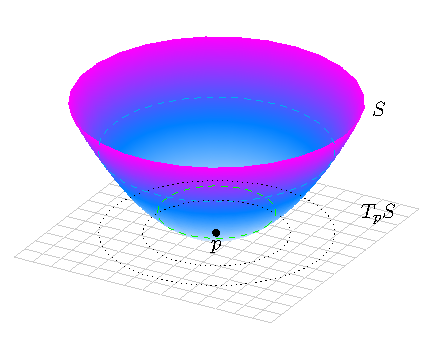
\includegraphics{picture/week9/curvature geo meaning.pdf}
            \begin{comment}
            \begin{tikzpicture}
                \begin{axis}[xticklabels={,,},%不显示x坐标轴数字
                    yticklabels={,,},
                    zticklabels={,,},
                    axis line style={draw=none},%不显示坐标轴
                    tick style={draw=none},
                    colormap/cool,
                    view={30}{40}
                ]
                \addplot3 [
                    surf,
                    domain=-1:1, domain y=-1:1,
                    samples=15, samples y=15,
                ] ({x},{y},{0});
                \addplot3[
                    surf,
                    shader=interp,
                    z buffer=sort,
                    domain=0:360, domain y=0:1,
                    samples=30, samples y=30,
                    variable=\u, variable y=\v,
                    ]({v*cos(u)},{v*sin(u)},{v*v});
                    \node[text=black] at (0,0,-0.1) {\(p\)};
                    \node at (0,0,0) {\(\bullet\)};
                    \node[text=black] at (0.8,0.8,0) {\(T_p S\)};
                    \node[text=black] at (0.8,0.8,0.8) {\(S\)};
                \addplot3 [
                    black,
                    dotted,
                    domain=0:360,
                    samples=30,
                    samples y=1%防止曲线闭合
                ]({0.8*cos(x)},{0.8*sin(x)},0);
                \addplot3 [
                    cyan,
                    dashed,
                    domain=0:360,
                    samples=30,
                    samples y=1%防止曲线闭合
                ]({0.8*cos(x)},{0.8*sin(x)},{0.64});
                \addplot3 [
                    black,
                    dotted,
                    domain=0:360,
                    samples=30,
                    samples y=1%防止曲线闭合
                ]({0.5*cos(x)},{0.5*sin(x)},0);
                \addplot3 [
                    green,
                    dashed,
                    domain=0:360,
                    samples=30,
                    samples y=1%防止曲线闭合
                ]({0.4*cos(x)},{0.4*sin(x)},{0.16});
                \end{axis} 
            \end{tikzpicture}
        \end{comment}
          \end{center}
          Then
          \[\label{geometric meaning curvature 2}
            K(p)=\lim_{r\to 0}3\frac{2\pi r-c(r)}{\pi r^3},\tag{2}  
          \]
          where \(c(r)\)= circumference of the circle of radius \(r\)
          on \(S\).
          \item Consider a disk around \(p\) of radius \(r\) in \(T_p S\). 
          Also consider a ``disk'' around \(p\) of radius \(r\) on 
          \(S\).
          \[\label{geometric meaning curvature 3}
            K(p)=\lim_{r\to 0} 12\frac{\pi r^2-A(r)}{\pi r^4},\tag{3}
          \]
          where \(A(r)\)= Area of disk on \(S\).
\end{enumerate}
\begin{remark}
    From expression of \cref{geometric meaning curvature 2} 
    and \cref{geometric meaning curvature 3}, one can prove 
    them by considering the Taylor's expansion of \(c(r)\)
    and \(A(r)\). The proof of these two facts will be postponed
     after we step into intrinsic geometry.(Need Taylor's expansion
      of metric tensor)
\end{remark}
\begin{proof}
    Let \(F(u,v)\) be the local parametrization on \(U\).
    \[
        \Rightarrow Area(U)=\iint_{F^{-1}(U)}\left|
            F_u\wedge F_v
        \right| \dd u\dd v,
    \]
    then \(T_{N(p)}N(U)=\Span\{N_u,N_v\}\),
    \[
        \bar{A}=\iint_{F^{-1}(U)} \left|N_u\wedge N_v\right|\dd u
        \dd v.
    \]
    \underline{Recall}: \(dN\begin{pmatrix}
        F_u\\
        F_v
    \end{pmatrix}=\begin{pmatrix}
        N_u\\N_v
    \end{pmatrix}=A\begin{pmatrix}
        F_u\\
        F_v
    \end{pmatrix}\), where \(A\) is the Weingarten matrix.
    \[
        \Rightarrow \left|
            N_u \wedge N_v
        \right|=\left|\det A\right|\left|
            F_u\wedge F_v
        \right|=|K|\left|
            F_u\wedge F_v
        \right|.
    \]
    \begin{align*}
        \frac{\bar{A}}{A}&=\frac{\iint |K|\left|
            F_u\wedge F_v
        \right|\dd u \dd v}{\iint \left|
            F_u\wedge F_v
        \right|\dd u\dd v}\\
        &=\frac{|K(q)|\left|
            F_u\wedge F_v
        \right|(q)Area(F^{-1}(U))}{\left|
            F_u\wedge F_v
        \right|(\bar{q})Area(F^{-1}(U))}\quad (\text{Middle value theorem}).
    \end{align*}
    As \(A\to 0\), \(q\to p\), \(\bar{q}\to p\),
    \[\Rightarrow |K(p)|=\lim_{A\to 0}\frac{\bar{A}}{A}.\]
\end{proof}
\section{More Examples}
\begin{exercise}
    Graph \(z=h(x,y)\)= \(S\). 
\end{exercise}
(\underline{Recall}: For a regular surface, by the implicit (inverse) 
function theorem, it can be written as a graph locally.)

In the HW 8, you may have computed 
\[
    I=\left(1+h_x^2\right)\dd x^2+2h_x h_y\dd x\dd y+(1+h_y^2)\dd y^2
\]
\[
    \II =\frac{h_{xx}}{\sqrt{1+\left|\nabla h\right|_{\mathbb{R}^2}^2}}
    \dd x^2 +2 \frac{h_{x}h_y}{\sqrt{1+\left|\nabla h
    \right|^2}}\dd x\dd y+\frac{h_{yy}}{\sqrt{1+\left|
        \nabla h\right|^2}}\dd y^2.
\]
\[
N=\frac{\left(-h_x,-h_y,1\right)}{\sqrt{1+\left|
    \nabla h\right|^2}}.    
\]
\[
    K=\frac{h_{xx}h_{yy}-h_{xy}^2}{\left(1+\left|
        \nabla h\right|^2\right)^2}=\frac{\det \nabla^2h}{\left(1+\left|
            \nabla h\right|^2\right)^2}.
\]
\[
    2H=\frac{(1+h_x^2)h_{yy}-2 h_x h_y h_{xy}+(1+h_y^2)h_{xx}}{
        \left(1+\left|
            \nabla h\right|^2\right)^{\frac{3}{2}}
    }    .
    \footnotemark
\]
\footnotetext{A basic observation one should make is how \(K\) and
\(H\) depend on the \engordnumber{2} derivative of \(h\).}
Note that the last term equals \[
    \mathrm{div}_{\mathbb{R}^2}\left(\frac{\nabla h}{
        \sqrt{1+\left|
            \nabla h\right|^2}
    }\right)
    =
    \sum_{i,j=1}^2 L^{ij}\left(\nabla f\right)\nabla_i\nabla_j h,
\]
where \[
    L^{ij}\left(\nabla f\right)=\frac{1}{\sqrt{1+\left|
        \nabla h\right|^2}}\left(\delta_{ij}-
        \frac{\nabla_i h\nabla_j h}{1+\left|
            \nabla h\right|^2}\right)    .
\]
Let \(p\in S\), and assume \(p\) is the origin in \(\mathbb{R}^3\),
 and \(N\) agrees with the unit normal of \(z\)-axis
 \[
    h_x=h_y=0\text{ at p}.   
 \]
 \[
    e=h_{xx}(0,0), f=h_{xy}(0,0), g=h_{yy}(0,0).   
 \]
 Hessian of \(h\) at \(p\) is 
 \[
    \begin{pmatrix}
        h_{xx}(0,0)& h_{xy}(0,0)\\
        h_{yx}(0,0)&h_{yy}(0,0)
    \end{pmatrix} .  
 \]
 Hence, at \(p\)
 \[
    \II=\mathrm{Hess}~h.   
 \]
 Moreover, at \(p\)
 \[
    \partial H=\delta h.
 \]
 As an application, we give a geometric interpretation of the Dupin
 indicatrix.
 \underline{Claim}: If \(p\in S\) is not a planar point, consider the 
 intersection of a plane parallel to \(T_p S\) with \(S\), and the plane
  is close enough to \(T_p S\), then the obtained curve is approximated
   by the Dupin indicatrix.
\begin{proof}
    Since we only care about local behavior at \(p\), W.L.O.G assume
     near \(p\), the surface is parametrized by the graph \(z=h(x,y)\),
     such that \(p\) is the origin and \(z\)-axis is the normal direction 
      and \(x\)-axis, \(y\)-axis are principal directions.
      Let the intersection curve be \(h(x,y)=\epsilon\), for sufficiently
      small \(\epsilon\). Consider the Tayler's expansion of 
      \(h(x,y)\) at \(p\)
      \begin{align*}
        h(x,y)=&h(0,0)+h_x(0,0)x+h_y(0,0)y\\
        &+\frac{1}{2}\left(
            h_{xx}(0,0)x^2+\underbrace{2h_{xy}(0,0)}_{
                =0\text{(principal direction)}
            }xy+h_yy(0,0)y^2
        \right)\\
        &+\text{Remainder}\\
        =&\frac{1}{2}\begin{pmatrix}
            x&y
        \end{pmatrix}
        \begin{pmatrix}
            h_{xx}(0,0)&0\\
            0&h_{yy}(0,0)
        \end{pmatrix}
        \begin{pmatrix}
            x\\
            y
        \end{pmatrix}+\text{Remainder},
      \end{align*}
\end{proof}
where 
\[
    \lim_{(x,y)\to (0,0)}    \frac{\text{Remainder}}{x^2+y^2}=0.
\]
Hence, the intersection curve is given by 
\[
    \frac{1}{2}\left(h_{xx}(0,0)x^2+h_{yy}(0,0)y^2\right)+R=\epsilon.    
\]
Note: in the \engordnumber{2} fundamental form\(II\) \(f=0\), 
and in the  \engordnumber{1} fundamental form \(I\) \(F=0\),
then at \(p\) one has 
\[
    \begin{cases}
        k_1=\frac{e}{E}=h_{xx}(0,0)\\
        k_2=\frac{g}{G}=h_{yy}(0,0)
    \end{cases}    
\]
using \(k_i=H\pm\sqrt{H^2-K}\). Then, \(k_1x^2+k_2y^2=2\epsilon\)
can be viewed as the \engordnumber{1} order approximation of the 
intersection curve. Renormalized it, then 
\[k_1 \bar{x}^2+k_2\bar{y}^2=1,\]
is just the Dupin indicatrix.
\begin{exercise}
    Surface of revolution.
\end{exercise}
Let \(\alpha(s)=\varphi(s),0,\psi(s)\) be a regular curve, with \(\varphi
(s)>0\) and \(s\in(a,b)\) is the arclength parametrization.
\(\Rightarrow \left(\varphi'(s)\right)^2+\left(\psi'(s)\right)^2=1\)
\(\Rightarrow \vphi'\vphi'' +\psi'\psi''=0\).
Rotate it about \(z\)-axis
\[
    \Rightarrow \alpha(\theta,s)=\left(\varphi(s)\cos\theta
    ,\varphi(s)\sin \theta,\psi(s)\right),\, 0<\theta<2\pi.
\]
\begin{align*}
    I=&\dd s^2+\varphi(s)^2\dd \theta^2\\
    \II=&\left(\psi'\vphi''-\psi''\vphi'\right)\dd s^2
    -\vphi\psi'\dd\theta^2.
\end{align*}
\(\because F=f=0\), \(\therefore\) \(s\)-curve and \(\theta\)-curve 
are curvature lines.
\[
    K=\frac{e}{E}\frac{g}{G}=-\frac{\varphi''}{\varphi},\;
    H=\frac{1}{2}\left(\frac{e}{E}+\frac{g}{G}\right)    .
\]
Since principal curvatures satisfy \(\lambda^2-2\lambda H+K=0\).
\[
    \Rightarrow \lambda_1    =\frac{e}{E}=-\frac{\vphi''}{\vphi},
    \;\lambda_2=\frac{g}{G}=\psi'\vphi''-\psi''\vphi'.
\]
The mean curvature is 
\[
    H=\frac{1}{2}\frac{-\psi'+\vphi\left(\psi'\vphi''-
    \psi''\vphi'\right)}{\vphi}.    
\]
\begin{question}[Homework]
    \begin{enumerate}[(1)]
        \item Assume \(K=1\), \(\lim_{s\to 0^+}\alpha(s)=(0,0,1)\),
         \(\alpha(\frac{\pi}{2})=(1,0,0)\),\(s\in (0,\pi)\). 
         Describe the surface and determine the \engordnumber{1}
         fundamental form (\(\dd s^2+\sin^2 s\dd \theta^2\)).
         \item Assume \(K=0\), \(\lim_{s\to 0^+}\alpha(s)=(0,0,1)\),
          \(\alpha(1)=(\frac{\sqrt{2}}{2},0,\sqrt{2}{2})\), 
          \(s\in (0,\infty)\), answer the same question as in (1)
          (\(\dd s^2+\frac{1}{2}s^2\dd \theta^2\)).
          \item Assume \(H=0\), \(\alpha(0)=(1,0,0)\), \(\alpha(1)
          =(\sqrt{2},0,\arcsin(1))\), \(s>0\), answer the question in 
          (1). (\(\alpha(s)=\left(\sqrt{1+s^2},0,\arcsin s\right)\),
           \(I=\dd s^2+(1+s^2)^2\dd \theta^2\sim \text{Catenoid}\)).
    \end{enumerate}
\end{question}

\begin{exercise}[Ruled surface]
    A line passing through a point \(\alpha_0\in\mathbb{R}^3\) 
    with direction \(v\in \mathbb{R}^3\) can be written as 
    \[
        \ell(t)=\alpha_0 + t v.    
    \]
    Now we let \(\alpha_0,v\) are two vector-valued functions,
    \ie\ \(\alpha(s),v(s)\), then the collection of lines form 
    a surface 
    \[
        R(s,t)=\alpha(s)+t v(s).    
    \]
Surfaces with such parametrization is called the ruled surfaces, 
where \(\alpha(s)\) is called the base curve of \(S\) and 
\(v(s)\) is called the director curve.
\end{exercise}
\begin{remark}
    Ruled surface may contain singular points.
\end{remark}
\begin{example}
    \(R(s,t)=\alpha(s)+t e_3\). \(\alpha(s)\) is the circle on \(x-y\)
    plane, \(e_3=(0,0,1)\). (\(x^2+y^2=1\)) 
    \begin{center}
        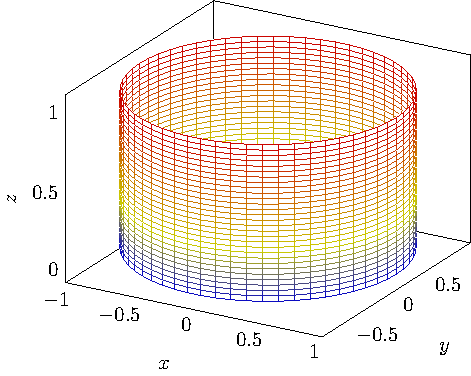
\includegraphics{picture/week9/ruled surface-cylinder.pdf}
        \begin{comment}
            \begin{tikzpicture}
    \begin{axis}[
        %xticklabels={,,},%不显示x坐标轴数字
        %yticklabels={,,},
        %zticklabels={,,},
        %axis line style={draw=none},%不显示坐标轴
        tick style={draw=none},
        view={30}{30},
        xlabel=\(x\),
        ylabel=\(y\),
        zlabel=\(z\)
    ]
    \addplot3 [
        surf,
        fill=white,
        domain=0:1, domain y=0:180,
        samples=30, samples y=30,
    ] ({cos(y)},{sin(y)},{x});
    \addplot3 [
        surf,
        fill=white,
        domain=0:1, domain y=180:360,
        samples=30, samples y=30,
    ] ({cos(y)},{sin(y)},{x});
    \end{axis}
\end{tikzpicture}
        \end{comment}
        \end{center}
\end{example}
\begin{example}\label{a ruled surface}
    \(R(s,t)=\alpha(s)+t\left(\alpha'(s)+e_3\right)\), where \(\alpha(s)\)
     and \(e_3\) are the same as before.
    \begin{center}
        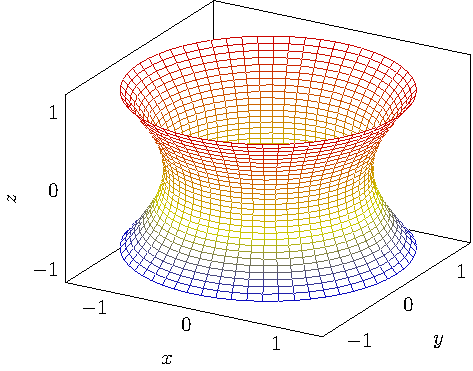
\includegraphics{picture/week9/ruled surface-catenoid.pdf}
        \begin{comment}
            \begin{tikzpicture}
    \begin{axis}[
        %xticklabels={,,},%不显示x坐标轴数字
        %yticklabels={,,},
        %zticklabels={,,},
        %axis line style={draw=none},%不显示坐标轴
        tick style={draw=none},
       % colormap/cool,
        view={30}{30},
        xlabel=\(x\),
        ylabel=\(y\),
        zlabel=\(z\)
    ]
    \addplot3 [
        surf,
        fill=white,
        domain=-1:1, domain y=0:180,
        samples=30, samples y=30,
    ] ({sqrt(x*x+1)*cos(y)},{sqrt(x*x+1)*sin(y)},{x});
    
    \addplot3 [
        surf,
        fill=white,
        domain=-1:1, domain y=180:360,
        samples=30, samples y=30,
    ] ({sqrt(x*x+1)*cos(y)},{sqrt(x*x+1)*sin(y)},{x});
\end{axis}
\end{tikzpicture}
        \end{comment}
    \end{center}
\end{example}
\begin{example}
    \(R(s,t)=0+t\left(u(s)+e_3\right)\), where \(u(s)=\left(
        \cos\theta,\sin\theta,0
    \right)\)
    \begin{center}
        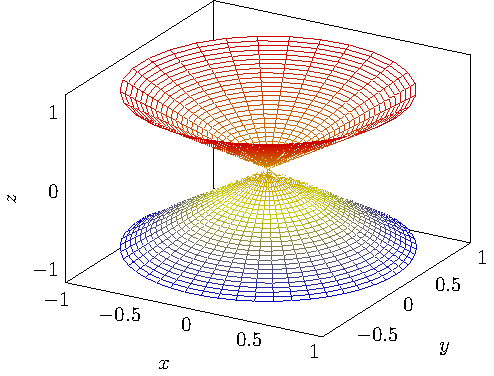
\includegraphics{picture/week9/ruled surface-cone.pdf}
        \begin{comment}
            \begin{tikzpicture}
    \begin{axis}[
        %xticklabels={,,},%不显示x坐标轴数字
        %yticklabels={,,},
        %zticklabels={,,},
        %axis line style={draw=none},%不显示坐标轴
        tick style={draw=none},
        view={30}{30},
        xlabel=\(x\),
        ylabel=\(y\),
        zlabel=\(z\)
    ]
    \addplot3 [
        surf,
        fill=white,
        domain=0:1, domain y=0:360,
        samples=30, samples y=30,
    ] ({x*cos(y)},{x*sin(y)},{x});
    \addplot3 [
        surf,
        fill=white,
        domain=-1:0, domain y=300:340,
        samples=30, samples y=30,
    ] ({x*cos(y)},{x*sin(y)},{x});
    \addplot3 [
        surf,
        fill=white,
        domain=-1:0, domain y=-30:180,
        samples=30, samples y=30,
    ] ({x*cos(y)},{x*sin(y)},{x});
    
    \end{axis}
\end{tikzpicture}
        \end{comment}
    \end{center}
\end{example}
In the following discussion, we assume the ruled surface \(S\)
\[
    R(s,t)=\alpha(s)+t v(s),~|v(s)|=1,~v'(s)\neq 0\forall s.    
\]
Direct computation shows:
\begin{align*}
    I=&\left|\alpha_s+t v_s\right|^2\dd s^2+2\left\langle
        \alpha_s,v
    \right\rangle \dd s\dd t
    +\dd t^2\\
    N=&\frac{\alpha_s\wedge v+t v_s \wedge v}{
        \left|\alpha_s\wedge v+t v_s \wedge v\right|
    }\\
    \II=&e\dd s^2+2f \dd s \dd t .
\end{align*}
Hence,
\[
    K=-\frac{f^2}{\det I}\le 0.    
\]
Note that 
\begin{align*}
    f&=\left\langle R_{st},N\right\rangle\\
    &=v_s\vdot \frac{\alpha_s\wedge v+t v_s \wedge v}{
        \left|\alpha_s\wedge v+t v_s \wedge v\right|
    }\\
    &=\frac{\left(v_s,\alpha_s,v\right)}{\left|R_s\wedge R_t\right|}.
\end{align*}
\begin{definition}
    \(S\) is called developable on ``flat'' surface if \(\left(
        v_s,v,\alpha_s
    \right)\equiv 0\). In this case \(K=0\).
\end{definition}
\begin{remark}
    Physically, a developable surface can be flattened onto a plane 
    without ``stretching'' or ``compressing'', but allowing unfolding
    or cutting along a line. Later, we'll see on page 414, section 5-8
    in Do Carmo: If on a developable surface \(S\), all lines can be 
    extended on both sides, the surface can only be a plane 
    or a cylinder.
\end{remark}
\begin{remark}
    On a non-cylindrical ruled surface \(S\), \ie\ 
    \[R(s,t)=\alpha(s)+t v(s),v'(s)\neq 0\forall s,\]
    one can choose a spherical base curve \(\beta(s)\) such
    that 
    \[
        R(s,t)=\beta(s)+t v(s),    
    \]
    where \(\left\langle\beta'(s)+v'(s)\right\rangle=0\),
     such curve is called the line of striction. Points on the line
      of striction is called the central points of the ruled surface.
\end{remark}
\begin{example}
    In \cref{a ruled surface}, \(\alpha(s)\) is the line of striction.
\end{example}
\begin{exercise}
    Find the line of restriction (\(\beta(s)-\alpha(s)
    -\frac{\left\langle\alpha',v'\right\rangle}{|v'|^2}v\)).
    Then \(R(s,u)=\beta(s)+u v(s)\).

    Hence, if we let \(\lambda=\frac{(\beta',v,v')}{|v'|^2}\), then 
    \(K=-\frac{\lambda^2}{\left(\lambda^2+u^2\right)^2}\).
\end{exercise}
\begin{exercise}[Homework]
    Prove that there are no closed smooth minimal surface in 
    \(\mathbb{R}^2\).
\end{exercise}
\begin{proof}
    On a closed surface, there must exist an elliptic point, at which 
    \(k>0\), this contradicts to minimal surface.
\end{proof}
\begin{theorem}
    \begin{enumerate}[(1)]
        \item If a surface of revolution \(M\) is minimal, then 
        \(M\) is contained in either a plane or a catenoid.
        \item If a ruled surface \(M\) is minimal, then \(M\) is 
        contained in either a plane or a helicoid.
    \end{enumerate}
\end{theorem}
\begin{proof}
    See homework.
\end{proof}
\section{Isometries between surfaces}
From this lecture on, we'll study the intrinsic geometry of a regular 
surface. More precisely, we'll see how the \engordnumber{1} fundamental
form determines the geometry.
\begin{itemize}
    \item \(S_1,S_2\) are regular Surfaces, \(f\colon S_1\to S_2\).
\end{itemize}
\begin{enumerate}[(1)]
    \item \(f\) is isomorphism (1-1 and onto) 
    (of sets)\(\Leftrightarrow \)
    \(S_1\) and \(S_2\) are identified as sets.
    \item \(f\) is homeomorphism (\(f\) is an isomorphism + \(f\)
    and \(f^{-1}\) continuous)\(Leftrightarrow\) \(S_1\) and \(S_2\)
    are identified as topological spaces.
    \item \(f\) is diffeomorphism (\(f\) is a homeomorphism+
    \(f,f^{-1}\) are smooth) \(\Leftrightarrow\) \(S_1\) and \(S_2\)
    are identified with considering smooth structures on them.
    \item \(f\) is isometry 
    
    \(\Leftrightarrow\) \(f\)
    is a diffeomorphism and \(f\) preserves the arclength, 
    area, angles,\(\ldots\)(everything defined by the 
    \engordnumber{1} fundamental form).
\end{enumerate}
\begin{definition}[Isometry]
    \(\vphi\colon S_1\to S_2\) is a diffeomorphism between regular 
    surfaces. If \(\forall p\in S_1\), \(v_1,v_2\in T_p S\)
    \[
        \left\langle v_1,v_2\right\rangle_p=
        \left\langle d\vphi_p(v_1),d\vphi_p(v_2)\right\rangle,
        \tag{1}\label{definition of isometry}
    \]
    which is equivalent to saying that \(\vphi\) preserves the 
    \engordnumber{1} fundamental form, then we say \(\vphi\) is 
    an isometry.
\end{definition}
\begin{definition}[Local isometry]
    \(\vphi\colon S_1\to S_2\) is called a local isometry, if 
    \(\forall p\in S_1\), \(\exists\) a neighborhood \(U\) of 
    \(p\) such that \(\vphi|_U\) is an isometry.
\end{definition}
\begin{example}
    Catenoid and helicoid are only locally isometric to each other but not 
    global isometric. In fact the helicoid is simply connected, but 
    the catenoid is not (since it comes from revolution).
\end{example}
\begin{remark}
    Isometry implies local isometry, however the converse is false.
\end{remark}
\begin{example}
    \(\left(\mathbb{R}^2,\dd x^2 +\dd y^2\right)\) and the cylinder 
    \((\cos u,\sin u,v), \dd u^2+\dd v^2\) are only local isometric
     to each other, but not ``globally'' isometric.

    (The local isometry map is just the local parametrization
    of cylinder:
    \[
        \vphi\colon (u,v,0)\to (\cos u,\sin u,v).    
    \]
    Clearly, \(\mathbb{R}^2\) and the cylinder are not diffeomorphic
    to each other, since the cylinder has a non-shrinkable loop.)
\end{example}
\begin{exercise}
    The condition in \cref{definition of isometry} is equivalent to 
    \[
        \forall w\in T_p S, \quad |w|_p=\left|d \vphi_p(w)
        \right|_{\varphi(p)}.\tag{2}\label{second definition of isometry}
    \]
\end{exercise}
\begin{proof}
    \cref{definition of isometry} \(\Rightarrow\)
     \cref{second definition of isometry}, obviously.

     \cref{second definition of isometry}
     \(\Rightarrow\) \cref{definition of isometry}, 
     let  \(w=v_1+v_2\), then 
     \[
        |w|_p^2=\left|d \vphi_p(w)
        \right|_{\varphi(p)}^2,~
        |v_1|_p^2=\left|d \vphi_p(v_1)
        \right|_{\varphi(p)}^2,~ 
        |v_2|_p^2=\left|d \vphi_p(v_2)
        \right|_{\varphi(p)}^2
     \]
     \[\Rightarrow
        \left\langle v_1,v_2\right\rangle_p=
        \left\langle d\vphi_p(v_1),d\vphi_p(v_2)\right\rangle.
     \]
\end{proof}
\begin{remark}
    If \(\vphi\colon S_1\to S_2\) is a local isometry.
    \(\forall p\in S_1\), let \(U\) be a coordinate patch of 
    \(p\) and \(\vphi|_U\colon U\to \vphi(U)\) is a diffeomorphism 
    given by 
    \[
        \vphi(u,v)=\left(\tilde{u},\tilde{v}\right).    
    \]
    \[
        I_1=\begin{pmatrix}
            \dd u& \dd v
        \end{pmatrix}
        \begin{pmatrix}
            E&F\\
            F&G
        \end{pmatrix}
        \begin{pmatrix}
            \dd u\\
            \dd v
        \end{pmatrix}
    \]
    \[
        I_2=\begin{pmatrix}
            \dd \tilde{u}& \dd \tilde{v}
        \end{pmatrix}
        \begin{pmatrix}
            \tilde{E}&\tilde{F}\\
            \tilde{F}&\tilde{G}
        \end{pmatrix}
        \begin{pmatrix}
            \dd \tilde{u}\\
            \dd \tilde{v}
        \end{pmatrix}.
    \]
    Note 
    \[
        \begin{pmatrix}
            \dd \tilde{u}\\
            \dd \tilde{v}
        \end{pmatrix}
        =
        \pdv{(\tilde{u},\tilde{v})}{(u,v)}
        \begin{pmatrix}
            \dd u\\
            \dd v
        \end{pmatrix}
        =
        J_\vphi 
        \begin{pmatrix}
            \dd u\\
            \dd v
        \end{pmatrix}    
    \]
    \[
        \Rightarrow 
        \begin{pmatrix}
            E&F\\
            F&G
        \end{pmatrix}=
        J_\vphi^\top \begin{pmatrix}
            \tilde{E}&\tilde{F}\\
            \tilde{F}&\tilde{G}
        \end{pmatrix} J_\vphi. 
    \]
\end{remark}
\begin{proposition}
    \(U\subset \mathbb{R}^2\), assume \(\gamma_1(U)\subset S_1\), 
    \(\gamma_2(U)\subset S_2\) are two local parametrizations 
    of \(S_1\) and \(S_2\) such that 
    \[
        E_1=E_2,~F_1=F_2,~G_1=G_2,    
    \]
    then \(\vphi=\gamma_2\circ \gamma_1^{-1}\) is a local isometry.
\end{proposition}
\begin{proof}
    \(\gamma_1,\gamma_2\) are local parametrizations \(\Rightarrow\)
    \(\vphi=\gamma_2\circ\gamma_1^{-1}\) is a local diffeomorphism. 
    It suffices to show \(\forall p\in U\), \(w\in T_p U\)
    \[
        I_p(w,w)=I_{\vphi(p)}(d\vphi_p(w),d\vphi_p(w)).    
    \]
    Let \(w=\alpha'(0)\in T_p S\) for a curve \(\alpha(t)\in S_1\),
     \(\alpha(t)=\gamma_1\left(u(t),v(t)\right)\) 
     \[\Rightarrow
     w=\pdv{\gamma_1}{u}u'(0)+\pdv{\gamma_1}{v}v'(0)\]
     \[
        I_p(w,w)=E_1u'(0)^2+2 F_1u'(0)v'(0)+G_1 v'(0)^2.   
     \]
     Since
     \[
        d\vphi_p(w)=\left.\dv{t}\right|_{t=0}\vphi\circ \alpha(t)
        =\pdv{\gamma_2}{u}u'(0)+\pdv{\gamma_2}{v}v'(0) ,
     \]
     \[
        \therefore I_{\vphi(p)}(d\vphi_p(w),d\vphi_p(w))=
        E_2 u'(0)^2+2 F_2 u'(0)v'(0)+G_2 v'(0)^2  .
     \]
    By assumption, \(I_p(w,w)=I_{\vphi(p)}(d\vphi_p(w),d\vphi_p(w))\).
\end{proof}
\begin{remark}
    For two (local) isometric surfaces \(S_1\) and \(S_2\), the 
    \engordnumber{1} fundamental forms might look quite different 
    in the given parametrization. But we can always find a coordinate 
    change on one of then to get the desired isometry between them.
    (Such coordinate change gives the isometry on the surface to itself)
\end{remark}
\begin{exercise}
    In your homework 6, you have checked the catenoid and the with 
    \[
        C(u,v)=\left(a\cosh v\cos u,a\cosh v\sin u,a v\right),~
        0<u<2\pi,~-\infty<v<+\infty
    \]
    and the helicoid with 
    \[
        H(\bar{u},\bar{v})=\left(\bar{v}\cos\bar{u},
        \bar{v}\sin\bar{u},a \bar{u}\right),~0<\bar{u}<2\pi,-\infty<
        \bar{v}<+\infty
    \]
    are local isometric, and the local isometry is 
    \[
        \vphi(u,v)=(\bar{u},\bar{v}),~\bar{u}=u,~\bar{v}=a\sinh v.    
    \]
\end{exercise}
\begin{remark}
    If \(\varphi\colon S_1\to S_2\) is an isometry, \(\vphi\) preserves distance, 
    length, angle, area et.c.
\end{remark}
We often use another weaker equivalent condition, \ie\ a diffeomorphism 
only preserving angle.
\begin{definition}
    A diffeomorphism \(\varphi\colon S_1\to S_2\) is called a conformal
    map if \(\forall p \in S_1\), \(v_1, v_2, \in T_p S_1\), we 
    have 
    \[
        \left\langle d\vphi_p(v_1),d\vphi_p(v_2)\right\rangle=
        \lambda^2(p)\left\langle v_1,v_2\right\rangle_p,
    \]
    where \(\lambda^2\) is a nowhere vanishing smooth function on \(S_1\)
    and \(S_1\) is said to be conformal to \(S_2\).
\end{definition}
\begin{definition}[Locally conformal]
    \(\vphi\colon S_1\to S_2\) is called a locally conformal map,
    if \(\forall\), \(\exists\) a neighborhood \(U\) of \(p\) such
    that  \(\vphi|)U\) is a conformal map.
\end{definition}
\begin{proposition}
    \(\vphi \colon S_1\to S_2\) is a locally conformal map if and only 
    if \(\vphi\) is an angle preserving smooth map.
\end{proposition}
\begin{proof}
    See homework.
\end{proof}
\begin{remark}
    \begin{enumerate}[(1)]
        \item Angle-preserving is a geometric description
        of (locally) conformal condition. In reality, it's more convenient
        to use definition.
        \item Conformal is also an equivalent relation on regular surfaces.
    \end{enumerate}
\end{remark}
\begin{example}
    In HW 6, you have checked that stereographic map
    \[
        \pi_N\colon \mathbb{S}^2-{N}\to \mathbb{R}^2   
    \]
    \[
        (x,y,z)\mapsto (\frac{x}{1-z},\frac{y}{1-z})    ,
    \]
    is a locally conformal map.
    Recall 
    \begin{align*}
        \dd s_{\mathbb{S}^2}^2&=\frac{4}{(1+u^2+v^2)^2}\left(
            \dd u^2+\dd v^2
        \right)\\
        &=\frac{4}{(1+u^2+v^2)^2}\dd s_{\mathbb{R}^2}^2
    \end{align*}
\end{example}
\begin{definition}[Locally conformal flat]
    A regular surface is called locally conformally flat, if 
    \(\forall p\in S\) \(\exists\) neighborhood \(U\) of \(f\)
    such that \(U\) is conformally equivalent to an open subset
    of \(\mathbb{R}^2\), \ie\ on \(U\) the first fundamental form of 
    \(S\) is 
    \[
        I_U=\lambda^2I_{\mathbb{R}^2}    
    \]
    for a non-vanishing smooth function.
\end{definition}
A remarkable result in surface theory is: 
\begin{theorem}
    Any regular surface is locally conformally flat.
\end{theorem}
In practice, this is very useful. The theorem tells that 
\(\forall p \in S\), we can choose a local parametrization
near \(p\) such that 
\[
    \dd s^2=\lambda^2\dd s_{\mathbb{R}^2}^2=\lambda^2\left(
        \dd x^2+\dd y^2
    \right).
\]
Such parametrization is called Isothermal parametrization.
Hence, the study of geometry on \(S\) (which is determined by the
\engordnumber{1} fundamental form) becomes the study of function
\(\lambda\).
\begin{proof}
    (Skip) (Reference: S.S. Chern, 1955, proceedings, An elementary 
    proof of the existence of isothermal parameters on a surface). 
    The proof is reduced to solving some complex valued differential
    equations
\end{proof}
\begin{remark}
    Later, in Riemannian Geometry course, you'll see there is a
    ``mysterious'' curvature  (Weyl) tensor to characterize the 
    ``locally conformally flat'' condition, \ie\ 
    \[\text{Weyl tensor}\equiv 0\Leftrightarrow \text{Locally 
    conformally flat}.\]
    However, Weyl tensor is always zero on a manifold of dimension
    2 and 3.
\end{remark}
\begin{remark}
    \begin{enumerate}[(1)]
        \item In surface theory, conformal map is closely related to
         the complex analysis.
        \item In higher dimensional Riemannian Geometry, there is a
        branch called conformal geometry.
    \end{enumerate}
\end{remark}

\underline{Yamabe Problem}:
\begin{enumerate}[(1)]
    \item Let \((M,g)\) be a close Riemannian manifold with 
    \(\dim M\ge 3\). Does there exist a Riemannian metric
    \(\tilde{g}\) such that \(\tilde{g}=\lambda^2 g\) and the 
    ``scalar curvature'' of \(\tilde{g}\) is a constant c?(\(c<0\)
    and \(c=0\) are solved. \(c>0\) remains open)
    \item In \(\dim =2\), this question is equivalent to 
    finding a metric with constant Gaussian curvature on a closed
    surface under the conformal change.
\end{enumerate}

\chapter{Intrinsic geometry}
\section{Einstein convention}

Recall \(v\in \mathbb{R}^n\), \(v=(v^1,\ldots,v^n)\implies v=\sum_{i=1}^n v^i e_i\).
\begin{enumerate}[(1)]
    \item The summation is taken over \(i=1,2,\ldots,n\);
    \item \(v=\sum_{i=1}^n v^ie_i=\sum_{j=1}^nv^je_j\), expression of \(v\) is
        independent of choice of summation indices \(i\) or \(j\).
    \item One ``\(i\)'' appears as upper index, another ``\(i\)'' appears as lower
        index.
\end{enumerate}

Einstein convention: Whenever there is pair of same letter as upper and a lower
index, then the expression is summation of the index letter from 1 to \(n\),
\(n\) is usually the dimension of vector space / manifold / etc.

\begin{example}
\begin{itemize}
    \item \(W=V\cdot A\), \(A=(A_i^j)_{n\times n}\) matrix, \(v,w\in \mathbb{R}^n\),
        then \[
            W^j=v^i A_i^j=\sum_{i}v^iA_i^j
        .\] 
    \item \[
        g^{ij}\omega_{jk}=\sum_{j=1}^n g^{ij}\omega_{jk}.
    .\] Where \(g^{ij}\) is the \((i,j)\)-entry of inverse matrix \(g^{-1}\) of
    \(g\). \ie\ \[
        g^{ij}g_{jk}=\delta^i_k,
        \quad g^{ij}g_{ij}=\sum_{i=1}^n \sum_{j=1}^{n}g^{ij}g_{ij}
        =\sum_{i=1}^{n}\delta^i_i=n
    .\] 

    We will use Einstein convention from now on.
\end{itemize}
\end{example}

\section{Therema Egregium (Gauss)}

\underline{Goal:} The Gaussian curvature \(K\) depends only on the 1st fundamental
form.

Previously, we have seen once we know local parametrization \(\vphi(x^1,x^2)\) of
a surface \(S\), then \(I,\II\) can be computed and the Gaussian curvature is \[
    K=\frac{\det \II}{\det I}=\frac{eg-f^2}{EG-F^2}
.\] Now, we want to follow the same procedure as we study the Frenet formula of a
curve and try to understand the motion of equation of frame \(\vphi_1,\vphi_2,N\),
where \(\vphi_i=\pdv{\vphi}{x^i}, N=\frac{\vphi_1\times \vphi_2}{|\vphi_1\times 
\vphi_2|}\).

Fix a local parametrization \[
    \vphi\colon U \longrightarrow S\subset \mathbb{R}^3,
    \ (x^1,x^2)\longmapsto \vphi(x^1,x^2)
.\] Then
\begin{align*}
    I&=g_{ij}\dd{x^i}\dd{x^j},\quad g_{ij}=\left<\vphi_i,\vphi_j\right> \\
    \II&=h_{ij}\dd{x^i}\dd{x^j},\quad h_{ij}
.\end{align*}
We shall study the differential equation of \(\{\vphi_i,N\}\) up to 2nd order.
\begin{align*}
    \vphi_{11}&=\Gamma_{11}^1\vphi_1+\Gamma_{11}^2\vphi_2+h_{11}N\\
    \vphi_{12}&=\Gamma_{12}^1\vphi_1+\Gamma_{12}^2\vphi_2+h_{12}N\\
    \vphi_{21}&=\Gamma_{21}^1\vphi_1+\Gamma_{21}^2\vphi_2+h_{21}N\\
    \vphi_{22}&=\Gamma_{22}^1\vphi_1+\Gamma_{22}^2\vphi_2+h_{22}N\\
.\end{align*}
Weingarten equation, \(A=(a_i^j)\)
\[
    \begin{bmatrix}
        N_1 \\ N_2
    \end{bmatrix}=A\begin{bmatrix}
        \vphi_1 \\ \vphi_2
    \end{bmatrix}
.\] Then \[
    a_i^j=-h_{ik}g^{kj}
.\] Lets write above equations as
\begin{equation}\label{eq:motion}
    \begin{cases}
        \vphi_{ij}=\Gamma_{ij}^k\vphi_k+h_{ij}N \\
        N_i=a_i^j=\vphi_j
    \end{cases}
    \implies \text{The only unknown are }\Gamma_{ij}^k
.\end{equation}
Moreover, \[
    \vphi_{ij}=\vphi_{ji}\implies \Gamma_{ij}^k=\Gamma_{ji}^k
.\] \[
    \left<\vphi_{ij},\vphi_p\right> =\Gamma_{ij}^k \left<\vphi_k,\vphi_p\right> 
    =\Gamma_{ij}^kg_{kl}
.\] So
\begin{gather*}
    \pdv{g_{ip}}{x^j}-\left<\vphi_i,\vphi_{pj}\right> 
    =\left<\vphi_{ij},\vphi_p\right> =\Gamma_{ij}^kg_{kp} \\
    \pdv{g_{jp}}{x^i}-\left<\vphi_j,\vphi_{pi}\right> 
    =\left<\vphi_{ji},\vphi_p\right> =\Gamma_{ji}^kg_{kp} \\
    \pdv{g_{ij}}{x^p}=\left<\vphi_{ip},\vphi_j\right>
    +\left<\vphi_i,\vphi_{jp}\right> 
\end{gather*}
Hence \[
    2\Gamma_{ij}^k g_{kp}=\pdv{g_{jp}}{x^i}+\pdv{g_{ip}}{x^j}-\pdv{g_{ij}}{x_{p}}
.\] \[
    \implies 2\Gamma_{ij}^kg_{kp}g^{pq}
    =(\pdv{g_{jp}}{x^i}+\pdv{g_{ip}}{x^j}-\pdv{g_{ij}}{x_{p}})g^{pq}
.\] We get \[
    \Gamma_{ij}^k=\frac{1}{2}(\pdv{g_{jp}}{x^i}+\pdv{g_{ip}}{x^j}g^{pk}
    -\pdv{g_{ij}}{x_{p}})
.\] 

\begin{remark}
    We multiply \(g^{pk}\) form right because of the choice of row vector. In
    modern convention of the column vector, \[
        \Gamma_{ij}^k=\frac{1}{2}g^{kp}(\pdv{g_{jp}}{x^i}+\pdv{g_{ip}}{x^j}
        -\pdv{g_{ij}}{x_{p}})
    .\] 
\end{remark}
\begin{definition}
    \(\Gamma_{ij}^k\) is called the Christoffel symbols. They're uniquely determined
    by the 1st fundamental form.
\end{definition}

Next we derive the Gauss equation, we'll see the Gaussian curvature can be
expressed only in 1st fundamental form.

So far, we have obtained \[
    \vphi_{ij}=\Gamma_{ij}^k\vphi_k+h_{ij}N
    \quad\&\quad
    N_p=a_p^q\vphi_q
.\] Then we have
\begin{align*}
    \vphi_{ijp}&= \partial_p \Gamma_{ij}^k\vphi_k+\Gamma_{ij}^k\vphi_{kp}+
    \partial_p h_{ij} N+h_{ij}N_p \\
    &= \partial_p\Gamma_{ij}^k\vphi_k+\Gamma_{ij}^k(\Gamma_{kp}^q+h_{kp}N)
    +\partial_p h_{ij} N+h_{ij}a_p^q \vphi_q, \\
    \vphi_{ipj}
    &= \partial_j\Gamma_{ip}^k\vphi_k+\Gamma_{ip}^k(\Gamma_{kj}^q+h_{kj}N)
    +\partial_j h_{ip} N+h_{ip}a_j^q \vphi_q
.\end{align*}
The derivative is taken in \(\mathbb{R}^3\), so the two expression should be
the same, we got 
\begin{align*}
    \vphi_{ijp}-\vphi_{ipj}
    =&(\partial_p\Gamma_{ij}^k-\partial_j\Gamma_{ip}^k)\vphi_k+(\Gamma_{ij}^k
    \Gamma_{kp}^q-\Gamma_{ip}^k\Gamma_{kj}^q)\vphi_q+(h_{ij}a_p^q-h_{ip}a_j^q)
    \vphi_q &\text{(tangential)} \\
    &+(\Gamma_{ij}^kh_{kp}-\Gamma_{ip}^kh_{kj}+\partial_p h_{ij}-\partial_{j}
    h_{ip})N &\text{(normal)} \\
    =& 0
\end{align*}
\begin{remark}
    If the ambient space is not \(\mathbb{R}^n\), LHS should give curvature of
    the ambient space.
\end{remark}

Note that \(\vphi_i\) and \(N\) are perpendicular, we can split tangential part
and normal part of the equation, and use \(a_{p}^k=-h_{pq}g^{qk}\) we get:

Normal part:
\begin{equation}\label{eq:codazzi}
    \partial_p h_{ij}-\Gamma_{pi}^kh_{kj}=\partial_j h_{ip}-\Gamma_{ji}^kh_{kp}
.\end{equation}

Tangential part: \[
    (h_{ij}h_{pq}-h_{ip}h_{jq})g^{qk}
    =\partial_p \Gamma_{ij}^k-\partial_j\Gamma_{ip}^k
    +\Gamma_{ij}^l\Gamma_{lp}^k-\Gamma_{ip}^l\Gamma_{lj}^k
.\] multiply by \(g^{kr}\) we get
\begin{equation}\label{eq:gauss}
    h_{ij}h_{pq}-h_{ip}h_{jq}=
    g_{qk}\left(\partial_p \Gamma_{ij}^k-\partial_j\Gamma_{ip}^k
    +\Gamma_{ij}^l\Gamma_{lp}^k-\Gamma_{ip}^l\Gamma_{lj}^k\right)
.\end{equation}

\cref{eq:codazzi} is called the Codazzi equation and~\cref{eq:gauss} is called
the Gauss equation. Take \(i=j,p=q\) in Gauss equation, we see LHS becomes \[
    h_{ii}h_{pp}-h_{ip}h_{pi}=\det\begin{bmatrix}
        h_{ii} & h_{ip} \\
        h_{pi} & h_{pp}
    \end{bmatrix}
.\] For 2 dim case, if \(i\neq p\), this gives exactly \(\det\II\). Note RHS
is purely determined by \(I\), hence \(K=\frac{\det\II}{\det I}\) only depends
on \(I\), it is an intrinsic geometric quantity.

{\color{red}\large !} Gaussian curvature is the local geometric invariant of
surfaces.

We look back Codazzi equation, we can add a term as \[
    \partial_{p}h_{ij}-\Gamma_{pi}^kh_{kj}-\boxed{\Gamma_{pj}^kh_{ki}}
    =\partial_{j}h_{ip}-\Gamma_{ji}^kh_{kp}-\boxed{\Gamma_{jp}^kh_{ki}}
.\] In terms of covariant derivative \(\nabla\), this writes \[
    \nabla_p h_{ij}=\nabla_{j} h_{ip}
.\] \ie\ All 3 index of \(\nabla_p h_{ij}\) are symmetric.

\begin{remark}
    We don't need to memorize the Gauss-Codazzi equations precisely. It
    suffices to work it out step by step once we know local parametrization.
    And there is a much more simple form of the equations after we introduced
    notations in Riemannian geometry.
\end{remark}

We also call the Gauss-Codazzi equations are the integrability to solve
the equation of motion~\cref{eq:motion}.

\begin{theorem}[Fundamental theorem of surface theory (local)]\hfill\\
    Let \(U\subset \mathbb{R}^2\) be open, connected set. Given two quadratic
    form \(I=g_{ij}\dd{x^i}\dd{x^j}, \II=h_{ij}\dd{x^i}\dd{x^j}\), \st\ \(I\) is
    positively definite. Moreover, the Gauss-Codazzi equations are satisfied.
    Then there is a surface \(S\) in \(\mathbb{R}^3\) \st\ \(I,\II\) are the 1st
    and 2nd fundamental form of \(S\) with \(U\) a coordinate chart.

    The surface \(S\) is unique up to rigid motion.
\end{theorem}
\begin{proof}
    Skip. (Can be found in Do Carmo's book)
\end{proof}

\section{An invitation of Riemannian Geometry}
We have introduced the concept of smooth manifold \(M\), \ie\ \(M\) is a
topological manifold together with a smooth structure, given by a collection
of coordinate covering \(M=\bigcup_{\alpha}U_\alpha\) \st\ 
\begin{enumerate}[(1)]
    \item \(\vphi_\alpha\colon U_\alpha\to \vphi_\alpha(U_\alpha)\subset
        \mathbb{R}^n\), is homeomorphism.
    \item \(\forall\,\alpha,\beta\), \(U_\alpha\cap U_\beta\neq\emptyset
        \implies\) the transition function \(\vphi_\beta\circ \vphi_\beta^{-1}\)
        on \(U_{\alpha}\cap U_\beta\) is smooth.
\end{enumerate}
Each \((U_\alpha,\vphi_\alpha)\) is called a coordinate patch.

Now a basic question is how to take derivative on \(M\)? This question is
natural to be asked since we want to apply the technique in calculus to study
\(M\).

First, we need to know how to differentiate \(f\in C^\infty(M)\), this has been
done by introducing ``tangent vector'' \& ``tangent vector field''.

Recall a smooth vector field \(X\) on \(M\) is a smooth map sending \(p\in M\)
to a vector \(X_p\in T_pM\). Let \(\Gamma(TM)\) be set of all smooth vector
fields on \(M\). \(X_p\) is understood geometrically as \(\forall\,f\in C^\infty
(M)\), \[
    (Xf)(p)=X_p(f)=\eval{\dv{t}}_{t=0}f(\alpha(t))
    =\lim_{t\to 0}\frac{f(\alpha(t))-f(p)}{t}
.\] Where \(\alpha(t)\) is any curve with initial value \(p\) and initial
velocity \(X_p\). We temporarily take this definition and try to generalize
it to Lie derivative. Soon we shall take the viewpoint that \(X_p\) as first
order derivative and generalize it to covariant derivative.

\subsection{Lie derivative}
Now we want to take derivatives of vector fields. First let's consider \(M=
\mathbb{R}^n\). Let \(V,W\) be two smooth vector fields, \(p\in \mathbb{R}^n\),
and
\begin{equation}\label{eq:lie-diff-Rn}
    \mathrm{D}_{V_p}W(p)=\lim_{t\to 0}\frac{W(p+tV_p)-W(p)}{t}
.\end{equation}
This just means the rate of ``change of value of \(W\)'' w.r.t. the ``change
of points in the domain''.

There're two things to be paid more attention:
\begin{enumerate}[(1)]
    \item \(p+tV_p\in \mathbb{R}^n\) is defined via linear structure of
        \(\mathbb{R}^n\).
    \item \(W(p+tV_p)-W(p)\), again, the subtraction makes sense by the linear
        structure of \(\mathbb{R}^n\). In which, we can identify \[
            T_p \mathbb{R}^n\cong T_{p+tV_p}\mathbb{R}^n\cong \mathbb{R}^n
        .\] 
\end{enumerate}

Next we consider general \(M\) as a manifold, \(V,W\in \Gamma(TM)\). To
generalize~\cref{eq:lie-diff-Rn} to manifolds, we have to reconsider (1) and
(2).
\begin{enumerate}[(1)]
    \item Given \(p\) and initial velocity \(V_p\), we can choose a smooth
    curve \(\alpha(t)\) as a replacement of ``linear perturbation in
    \(\mathbb{R}^n\)''
    \item Then consider the vector field \(W\) (restricted on \(\alpha(t)\)).
    \ie\ \(W(\alpha(t))\in T_{\alpha_(t)}M\). However \(T_{\alpha(t)}\neq
    T_pM\), not the same linear space. To do the subtraction, we need to
    ``move'' \(W(\alpha(t))\) back to \(T_pM\). This can be done by viewing \[
        \alpha(t)\colon p \mapsto \alpha(t)
    \] as a smooth map from \(M\) to \(M\) (at least locally). Then we can
    define a map \[
        \alpha(-t)\colon \alpha_(t) \mapsto p.
        \quad\text{(again from }M\text{ to }M\text{)}
    \] We have
    \begin{align*}
        \dd{\alpha(-t)}_{\alpha(t)}\colon T_{\alpha(t)}M &\longrightarrow
        T_p M \\
        W(\alpha(t)) &\longmapsto \left(\dd{\alpha(-t)}\right)_{\alpha(t)}
        (W(\alpha(t)))\in T_p M
    .\end{align*}
    Then \(\left(\dd{\alpha(-t)}\right)_{\alpha(t)}(W(\alpha(t)))\) and \(W_p\)
    both live in \(T_p M\).
\end{enumerate}

\begin{definition}[Lie derivative] \[
    \mathcal{L}_V W(p):=\lim_{t \to 0} \frac{\left(\dd{\alpha(-t)}_{\alpha(t)}
    \right)(W(\alpha(t)))-W(p)}{t}
\] is called the Lie derivative of \(W\) along \(V\), of course, we can write
above as \[
    \mathcal{L}_V W(p):=\eval{\dv{t}}_{t=0}
    \left(\dd{\alpha(-t)}_{\alpha(t)}\right)(W(\alpha(t)))
.\] 
\end{definition}

Note that \(\mathcal{L}_V W\) is still a smooth vector field (Exercise). The
computational formula is given by
\begin{prop} \[
    \mathcal{L}_V W=\left[V,W\right]=VW-WV
.\] In some books, people just take this as the definition of Lie derivative.
\end{prop}

\([V,W]\) is called the Lie bracket, defined by \(\forall\,f\in C^\infty(M)\),
\[
    [V,W](f)=V(W(f))-W(V(f))
.\] One should check this do give a derivation and defines a smooth vector
field.

Note if we write \(\mathcal{L}_V f=V(f)\), then above equation writes \[
    (\mathcal{L}_V W)(f)=\mathcal{L}_V(W(F))-W(\mathcal{L}_V f)
.\] \ie\ \[
    \mathcal{L}_V(W(f))=(\mathcal{L}_V W)(f)+W(\mathcal{L}_V f)
.\] This is Leibniz rule for Lie derivative.

Locally, let \(V=V^i\pdv{x^i},W=W^j\pdv{x^j}\), then
\begin{align*}
    [V,W]&= [V^i\pdv{x^i},W^j\pdv{x^j}]=V^i\pdv{x^i}(W^j\pdv{x^j})
    -W^j\pdv{x^j}(V^i\pdv{x^i}) \\
    &= V^i\pdv{W^j}{x^i}\pdv{x^j}+V^iW^j\pdv{x^ix^j}
    -W^j\pdv{V^i}{x^j}\pdv{x^i}-W^jV^i\pdv{x^ix^j} \\
    &= V^i\pdv{W^j}{x^i}\pdv{x^j}-W^j\pdv{V^i}{x^j}\pdv{x^i} \\
    &= (V^i\pdv{W^j}{x^i}-W^i\pdv{V^j}{x^i})\pdv{x^j}
.\end{align*}

Let's pause to introducing Lie derivative until we need more properties of it.

\subsection{Affine connection \& Covariant derivative}
Now we take another viewpoint of tangent vector fields. \ie\ A smooth vector
field \(V\) on \(M\) is understood as a 1st order differential operator acting
on \(C^\infty(M)\). \ie\ \(V\in \Gamma(TM)\), \(f\in C^\infty(M)\), \(V(f)\) is
a smooth function \st\ \[
    V(f)(p)=V_p(f)
.\] where \(V_p\colon C^\infty(M)\to \mathbb{R}\) \st\ 
\begin{enumerate}[(1)]
    \item \(V_p(f+\lambda g)=V_p(f+\lambda V_p(g))\),
    \item \(V_p(fg)=V_p(f)g(p)+f(p)V_p(g)\).
\end{enumerate}
Lets also write \(V(f)=\nabla_V f\), then \(\forall\,V,W\in \Gamma(TM)\),
\(h\in C^\infty(M)\), we have \[
    \nabla\colon \Gamma(TM)\times C^\infty(M)\to C^\infty(M),
    \quad(V,f)\mapsto \nabla_V f,
\]
satisfies:
\begin{enumerate}[(1)]
    \item \(\nabla_{V+hW}f=\nabla_V f+h\nabla_W f\),
    \item \(\nabla_V(f+\lambda h)=\nabla_V f+\lambda \nabla_V h\),
    \item \(\nabla_V(fh)=(\nabla_V)h+f\nabla_V h\).
\end{enumerate}

In a similar fashion, we define the covariant derivative \(\nabla_V W\),
by requiring (1)-(3) above, more precisely, \(\forall\,V,W,Z\in \Gamma(TM),
f\in C^\infty(M),\lambda\in \mathbb{R}\),
\begin{enumerate}[(1)]
    \item \(\nabla_{V+fZ}W=\nabla_V w+f\nabla_Z W\). (\(C^\infty\)-linear
        in subscript vector filed)
    \item \(\nabla_V(W+\lambda Z)=\nabla_V W+\lambda\nabla_V Z\).
        (\(\mathbb{R}\)-linear in vector fields)
    \item \(\nabla_V(fW)=(\nabla_V f)W+f\nabla_V W\). (Leibniz rule)
\end{enumerate}

\begin{definition}
    \[\nabla\colon \Gamma(TM)\times \Gamma (TM)\to \Gamma(TM)\]
    \[(X,Y)\mapsto \nabla_X Y\]
    is called the affine connection on \(M\).
\end{definition}
\underline{Fact}: There are many such affine connections!

In practice, we need local expressions of \(\nabla_V W\). Let 
\((x^1,\ldots,x^n)\) be a local coordinate on \(U\subset M\), 
\(V=V^i\pdv{x^i},W=W^i\pdv{x^i}\), then
\begin{align*}
    \nabla_V W &=\nabla_{V^i\pdv{x^i}}\left(W^j\pdv{x^j}\right)\\
    &= V^i\nabla_{\pdv{x^i}}\left(W^j \pdv{x^j}\right)\\
    &=V^i\left(\left(\nabla_{\pdv{x^i}} W^j\right)\pdv{x^j}
    + W^j \nabla_{\pdv{x^i}} \pdv{x^j}\right)\\
    &=V^i\left(\pdv{W^j}{x^i}\pdv{x^j}+W^j
    \boxed{\nabla_{\pdv{x^i}}\pdv{x^j}}\right).
\end{align*}
\begin{definition}
    On \(U\), we define the Christoffel symbol by 
    \[
        \nabla_{\pdv{x^i}}\pdv{x^j}=\Gamma\indices*{_{ij}^k}\pdv{x^k}.
    \]
    (Here, one should compare this definition with the Christoffel
    symbol introduced in the study of equation of motion 
    in previous lectures).
\end{definition}
\[
    \Rightarrow \nabla_V W= V^i\left(\pdv{W^j}{x^i}+W^k\Gamma
    \indices*{_{ki}^j}\right)\pdv{x^j}   .
\]
Conventionally, we define
\[
    \nabla_i W^j=\pdv{W^j}{x^i}+\Gamma\indices*{_{ik}^j}W^k    
\]
\begin{itemize}
    \item \(\nabla_i W^j\): Taking covariant derivative 
    of \(j\)-th component of \(W\) along the \(i\)-th coordinate
    direction.
    \item \(\pdv{W^j}{x^i}\): Euclidean derivative.
    \item \(\Gamma\indices*{_{ik}^j}W^k\): Correction term.
\end{itemize}
This notion is frequently used in geometry references.

Again, because there are tons of selection of affine connections,
this yields many choices of \(\Gamma\indices*{_{ij}^k}\)!
After we introduce the Riemannian metric, we shall see there is a unique
affine connection compatible with the Riemannian metric.
\begin{definition}[Riemannian metric]
    Let \(M\) be a smooth manifold. A Riemannian metric on \(M\)
    is a smooth map 
    \[
     g\colon \Gamma(TM)\times \Gamma(TM)\to C^\infty(M),
    \]
    such that 
    \(\forall X,Y,Z\in \Gamma(TM), f\in C^\infty(M)\)
    there is the following 
    \begin{enumerate}[(1)]
        \item \(g(X,Y)=g(Y,X)\).(symmetry)
        \item \(g(X,X)\ge 0\), and equality achieves iff \(X=0\).
        (positive definite)
        \item \(g(f X+Y,Z)=f\cdot g(X,Z)+g(Y,Z)\).(\(C^\infty\) linearity) 
    \end{enumerate}
    \((M,g)\) is called a Riemannian manifold.
\end{definition}
\begin{remark}
    At each \(p\in M\), \(g\) defines an inner product \(g_p\)
    on \(T_p M\). If we choose a coordinate chart near \(p\)
    with local coordinate \((x^1,\ldots,x^n)\),
    the local expression of \(g\) is written as 
    \[
        g=g_{ij}dx^i dx^j    ,
    \]
    where \(g_{ij}=g\left(\pdv{x^i},\pdv{x^j}\right)\).
\end{remark}
\begin{example}
    The \engordnumber{1} fundamental form on \(M\) is a Riemannian metric.
\end{example}
Using the Riemannian metric \(g\), we can define 
the length, area, angle, et.c.
\begin{definition}
    \begin{enumerate}[(1)]
        \item \(X\in \Gamma(TM)\), \(|X|=\sqrt{g(X,X)}\).
        \item The volume density on \((M,g)\) is defined as 
        \[
            \dd V=\sqrt{\det(g_{ij})} dx^1\wedge\ldots \wedge dx^n .
        \]
        \item The volume of a bounded region \(B\) is 
        \[
            V(B)=\int_B 1 \dd V
        \]
    \end{enumerate}
\end{definition}
With the Riemannian metric introduced, we can uniquely determine
an affine connection compatible with the Riemannian metric.
\begin{theorem}
    Let \((M,g)\) be a Riemannian manifold, then there is a unique
    affine connection 
    \(\nabla\colon \Gamma(TM)\times \Gamma (TM)\to \Gamma(TM)\)
    satisfying following conditions: \(\forall X,Y,Z\)
    \begin{enumerate}[(1)]
        \item \(\nabla_Z \left(g(X,Y)\right)=g\left(
            \nabla_Z X,Y\right)+g(X,\nabla_Z Y)\).(Compatible with metric 
            \(g\))\footnotemark
        \item \(\nabla_X Y-\nabla_Y X=[X,Y]\).(Torsion free)
    \end{enumerate}
    \footnotetext{(1) is also equivalent to \(\nabla g=0\). 
    (We shall talk about this later)}
    The connection \(\nabla\) is called Levi-Civita connection.
\end{theorem}
Locally, take \(X=\pdv{x^i},Y=\pdv{x^j},Z=\pdv{x^k}\)
\begin{align*}
    (1)&\Rightarrow \pdv{g_{ij}}{x^k}=\Gamma\indices*{_{ki}^l}g_{lj}
    +\Gamma\indices*{_{kj}^l}g_{l i}    \\
    (2)&\Rightarrow \Gamma\indices*{_{ij}^k}=\Gamma\indices*{_{ji}^k}.
\end{align*}
\begin{exercise}
    Show that 
    \[
        \Gamma\indices*{_{ij}^k}=\frac{1}{2}g^{kl}\left(
            \pdv{g_{jl}}{x^i}+\pdv{g_{il}}{x^j}-\pdv{g_{ij}}{x^l}
        \right)    
    \]
    This is just the same expression as we see on.
    %打到这里的时候page142还不存在,到时候再做引用。
\end{exercise}
So far, we have defined \engordnumber{1} order derivatives (Lie derivative,
covariant derivative) on functions and vector fields. Next we shall consider
\engordnumber{2} order derivatives of a function and vector fields.
In particular, non-commutative nature of \engordnumber{2} order derivative
on vector fields will be captured by the ``curvature''.
    
Let's assume \(\nabla\) to be the Levi-Civita connection from now on.
\begin{itemize}
    \item Recall we have defined tangent bundle. 
    \(TM=\bigcup_{p\in M} T_p M\) is the collection of all 
    tangent vector spaces. As a vector space, \(T_p M\) is isomorphic 
    to \(\mathbb{R}^n\). Let \(T^*_p M=\)\{all covectors at \(p\)\}.
    We also let \(T^*M=\bigcup_{p\in M}T^*_p M=\bigcup_p 
    \left\{(p,\alpha)| \alpha\in T^*_p M\right\}\). Similar to the 
    \(TM\), one can endow a smooth structure on \(T^*M\) such that 
    it's a smooth manifold of dimension \(2\dim M\). We shall also 
    call an element of \(\Gamma(T^* M)\) a differential 1-form, 
    where \(\Gamma(T^*M)\) is the collection of all global covectors.
    \item We have introduced 
    \[
        \nabla \colon \Gamma(TM)\times C^\infty(M)\to C^\infty(M)
    \]
    \[
        (X,f)\mapsto \nabla_X f.    
    \]
    This map induces 
    \[
        \nabla f\colon \Gamma(TM)\to C^\infty(M).
    \]
    At each point \(p\in M\) this map is 
    \[
        X\mapsto \nabla_X f=\nabla f(X).    
    \]
    \(
        \nabla f(p)\colon T_p M\to \mathbb{R}\Rightarrow 
        \nabla f(p)\in T^*_p M\Rightarrow
        \nabla f\in \Gamma(T^* M)
    \).
\end{itemize}
\begin{remark}
    If \((x^1,\ldots, x^n)\) is local coordinate at \(p\). \(T_p M
    =\Span\{\pdv{x^1},\ldots,\pdv{x^n}\}\), then \(T^*_p M=\Span 
    \{d x^1,\ldots , d x^n\}\), \(dx^i\left(\pdv{x^j}\right)=\delta^i_j\)
    \[
        \Rightarrow \nabla f(p)=\pdv{f}{x^i} (p)dx^i=\nabla_i f\cdot 
        d x^i. \quad (\nabla_i f=\pdv{f}{x^i})    
    \]
\end{remark}
\begin{definition}
    The gradient vector field of \(f\), written as \(\mathrm{grad} f=
    \mathrm{grad}_g f \) is defined as \(\forall X\in \Gamma(TM)\)
    \[
        g(\mathrm{grad} f,X)=\nabla_X f=\nabla f(X).    
    \]
\end{definition}
Locally, 
\[
    \mathrm{grad} f=g^{ij}\pdv{f}{x^j}\pdv{x^i}=\nabla^i f\pdv{x^i}.
\]
\begin{definition}[Hessian of \(f\)]
    \[
        \nabla\nabla f\colon \Gamma(TM)\times \Gamma(TM)\to C^\infty(M)
    \]
    \[
        (X,Y)\mapsto \nabla\nabla f(X,Y).    
    \]
    Where \(\nabla\nabla f(X,Y)=\left(\nabla_X \nabla f\right)(Y)
    \footnotemark
    =\nabla_X
    \left(\nabla f(Y)\right)-\nabla f\left(\nabla_X Y\right)=
    X\left(Y f\right)-()\nabla_X Y) f\).
\end{definition}
\footnotetext{Note that here we haven't defined the covariant derivative of
 a 1-form}
 Locally: 
 \begin{align*}
    \nabla\nabla f\left(\pdv{x^i},\pdv{x^j}\right)&=
    \pdv{x^i}\left(\pdv{f}{x^j}\right)-\nabla_{\pdv{x^i}}\pdv{x^j} f\\
    &=\pdv{f}{x^i}{x^j}-\Gamma\indices*{_{ij}^k}\pdv{f}{x^k}.
 \end{align*}
 \begin{remark}
    \begin{enumerate}[(1)]
        \item We conventionally write \(\nabla\nabla f(\pdv{x^i}
        \pdv{x^j})=\nabla_i\nabla_j f\), \ie\ 
        \[
            \nabla_i\nabla_j f=
            \pdv{f}{x^i}{x^j}-\Gamma\indices*{_{ij}^k}\pdv{f}{x^k}.   
        \]
        \begin{itemize}
            \item \(\nabla_i\nabla_j f\): tensor component.
            \item \(\pdv{f}{x^i}{x^j}\): Euclidean Hessian.
            \item \(\Gamma\indices*{_{ij}^k}\pdv{f}{x^k}\)
            Correction.
        \end{itemize}
        \item \(\nabla_i\nabla_j f=\nabla_j\nabla_i f\).(Symmetric in 
        \(i\) and \(j\))
        \item In tensor notation we write this as 
        \[
            \nabla\nabla f=\left(\nabla_i\nabla_j f\right)d x^i d x^j.    
        \]
    \end{enumerate}
 \end{remark}
 \begin{definition}[Laplacian of \(f\)]
    \(\Delta f=\mathrm{trace}\left(\nabla\left(\mathrm{grad}
    f\right)\right)\).
 \end{definition}
 Locally, \(\mathrm{grad} f=\nabla^i f\pdv{x^i}\Rightarrow
 \nabla\left(\mathrm{grad}f\right)=\nabla_j\nabla^i f dx^j\otimes
  \pdv{x^i}\).
  \begin{align*}
    \Delta f & =\nabla_i \nabla^i f=g^{ij}\nabla_i\nabla_j f\\
    &=g^{ij}\left(
        \pdv{f}{x^i}{x^j}-\Gamma\indices*{_{ij}^k}\pdv{f}{x^k}
    \right).
  \end{align*}
  \begin{exercise}
    Show that 
    \[
        \Delta f=\frac{1}{\sqrt{\det g}}\pdv{x^i}\left(
            \sqrt{\det g}\cdot g^{ij}\pdv{f}{x^j}
        \right)    .
    \]
  \end{exercise}
  Note that the expression of R.H.S follows from
  ``integration by parts'', \ie\ \(\forall h\in C^\infty_c(M)\),
  \[
    \int_M  h\Delta f \sqrt{g}\dd x =-\int_M \left\langle
        \nabla h,\nabla f
    \right\rangle\sqrt{g}\dd x.
  \]
  Next, we consider taking \engordnumber{2} order derivative
  of a vector field \(Z\) along two different vector fields \(X\) and 
  \(Y\). Let's do a general local computation.(The following 
  computation should be very familiar with you)

  Let \(X=X^i\pdv{x^i},Y=Y^j\pdv{x^j},Z=Z^k\pdv{x^k}\)
  \begin{align*}
    \Rightarrow \nabla_X\nabla_Y Z&=
    \nabla_X\left(\nabla_Y Z\right)\\
    &=\nabla_X\left(\left(Y^j \nabla_j Z^k\right)\pdv{x^k}\right)\\
    &=\left(X^i\nabla_i Y^j\nabla_j Z^k+X^i Y^j\nabla_j\nabla_i Z^k
    \right)\pdv{x^k}\\
    \nabla_Y\nabla_X Z&=\left(Y^j\nabla_j X^i \nabla_i Z^k
    +X^iY^j \nabla_j\nabla_i Z^k\right)\pdv{x^k}
  \end{align*}
  \begin{align*}
    &\Rightarrow \nabla_X\nabla_Y Z-\nabla_Y\nabla_X Z\\
    &=
    X^i Y^j\left(\nabla_i\nabla_j Z^k-\nabla_j\nabla_i Z^k\right)
    \pdv{x^k}+\left(\nabla_{\nabla_X Y}Z^k-\nabla_{\nabla
    _Y X }Z^k\right)\pdv{x^k}\\
    &=X^i Y^j\left(\nabla_i\nabla_j Z^k-\nabla_j\nabla_i Z^k\right)
    \pdv{x^k}
    +\left(\nabla_{[X,Y]}Z^k\right)\pdv{x^k}.
  \end{align*}
  \(\therefore \nabla_X\nabla_Y Z-\nabla_Y\nabla_X Z -\nabla_{[X,Y]}Z=
  X^i Y^j\left(\nabla_i\nabla_j Z^k-\nabla_j\nabla_i Z^k\right)
    \pdv{x^k}
  \).
\begin{definition}
    The (1,3) Riemannian curvature tensor is defined by a map 
    \[
        R\colon \Gamma(TM)\times \Gamma(TM)\times \Gamma(TM)
        \to \Gamma(TM)    
    \]
    \[
        \left(X,Y,Z\right)\mapsto R(X,Y)Z    
    \]
    \[
        R(X,Y)Z=\nabla_X\nabla_Y Z-\nabla_Y\nabla_X Z -\nabla_{[X,Y]}Z    
    \]
    Locally, 
    \[
        R\left(\pdv{x^i},\pdv{x^j}\right)\pdv{x^k}=R\indices{_{ij}^l_k}
        \pdv{x^l}    
    \]
\end{definition}
\begin{exercise}
    \begin{enumerate}[(1)]
        \item Check \(R\) is \(C^\infty\) in \(X,Y,Z\).
        \item Find a local expression for \(R\indices{_{ij}^l_k}\)
        in terms of Christoffel symbols.
    \end{enumerate}
\end{exercise}
Computation: take \(X=\pdv{x^i}\), \(Y=\pdv{x^j}\), \(Z=\pdv{x^k}\),
\begin{align*}
    R\left(\pdv{x^i},\pdv{x^j}\right)\pdv{x^k}&=
    \nabla_i\nabla_j\pdv{x^k}-\nabla_j\nabla_i\pdv{x^k}\\
    &=\nabla_i\left(\Gamma\indices*{_{jk}^l}\pdv{x^l}\right)
    -\nabla_j\left(\Gamma\indices*{_{ik}^l}\pdv{x^l}\right)\\
    &=\left(\partial_i\Gamma\indices*{_{jk}^l}\right)\pdv{x^l}+
    \Gamma\indices*{_{jk}^l}\Gamma\indices*{_{il}^p}\pdv{x^p}
    -\partial_j\Gamma\indices*{_{ik}^l}\pdv{x^l}
    -\Gamma\indices*{_{ik}^l}\Gamma\indices*{_{jl}^p}\pdv{x^p}\\
    &=\left(\partial_i\Gamma\indices*{_{jk}^l}+
    \Gamma\indices*{_{jk}^p}\Gamma\indices*{_{ip}^l}-
    \partial_j\Gamma\indices*{_{ik}^l}-\Gamma\indices*{_{ik}^p}
    \Gamma\indices*{_{jp}^l}\right)\pdv{x^l}\\
    &=\left(\textcolor{blue}{
        \partial_i\Gamma\indices*{_{jk}^l}
        -\partial_j\Gamma\indices*{_{ik}^l}
        +\Gamma\indices*{_{jk}^p}\Gamma\indices*{_{ip}^l}
        -\Gamma\indices*{_{ik}^p}\Gamma\indices*{_{jp}^l}
    }
    \right)\pdv{x^l}
\end{align*}
\textcolor{olive}{
    \underline{Notation}: \(R\left(\pdv{x^i},\pdv{x^j}
    \right)\pdv{x^k}=\tensor{R}{_{ij}^l_k}\pdv{x^l}\).
    \[
        \tensor{R}{_{ij}^l_k}=
        \partial_i\Gamma\indices*{_{jk}^l}
        -\partial_j\Gamma\indices*{_{ik}^l}
        +\Gamma\indices*{_{jk}^p}\Gamma\indices*{_{ip}^l}
        -\Gamma\indices*{_{ik}^p}\Gamma\indices*{_{jp}^l}
    \]
}
\begin{definition}
    The (0,4) Riemannian curvature tensor is defined as 
    \[
        Rm:\Gamma(TM)\times \Gamma(TM)\times\Gamma(TM)\times\Gamma(TM)
        \to C^\infty(M) 
    \]
    \[
        (X,Y,W,Z)\mapsto Rm(X,Y,W,Z)=g\left(R(X,Y),Z,W\right)    
    \]
\end{definition}
Locally, \(\tensor{R}{_{ijlk}}=
R(\pdv{x^i},\pdv{x^k},\pdv{x^l},\pdv{x^k})=
g\left(R\left(\pdv{x^i},\pdv{x^j}\right)\textcolor{blue}{\pdv{x^k}}
,\textcolor{blue}{\pdv{x^l}}\right)=
g\left(\tensor{R}{_{ij}^p_k}\pdv{x^p},\pdv{x^l}\right)=
\tensor{R}{_{ij}^p_k}g_{pl}
\)
\[
    \textcolor{olive}{
        \Rightarrow \tensor{R}{_{ijlk}}=\tensor{R}{_{ij}^p_k}g_{pl}
        \text{ (pull-down the \engordnumber{3} index)},
    }
\]
\[
    \textcolor{olive}{
        \Rightarrow
        \tensor{R}{_{ij}^p_k}=
        \tensor{R}{_{ijlk}} g^{lp}
        \text{ (lift-up the \engordnumber{3} index)}.
    }    
\]
\begin{remark}
    For a pair of vector fields \(X,Y\), \(R(X,Y)=
    \left[\nabla_X,\nabla_Y\right]-\nabla_{[X,Y]}\) is an 
    antisymmetric (in \(X\) and \(Y\)) operator from 
    \(\Gamma(TM)\to \Gamma(TM)/\)
    \[\Rightarrow R(X,Y)\in End \left(\Gamma(TM)\right)=\Gamma
    \left(T^* M\otimes TM\right).\]
\end{remark}

\textcolor{blue}{
    \begin{definition}
        At \(p\in M\), let \(\pi\) be a 2-plane generated by \(v,w\in T_p W\),
    the sectional curvature of \(\pi\) is 
    \[
        K_p(\pi)=\frac{Rm(v,w,v,w)}{\Vert v\wedge w\Vert^2},    
    \]
    where \(\Vert v\wedge w\Vert^2=g(v,v)g(w,w)-g(v,w)^2\). (Area of 
    \(\pi\))
    \end{definition}
}

\textcolor{orange}{
    Important properties of (0,4) Riemannian curvature tensor: 
    \begin{enumerate}[(1)]
        \item \(Rm(\textcolor{blue}{X,Y},W,Z)=
        -Rm(\textcolor{blue}{Y,X},W,Z)\).
        \item \(
            Rm(\textcolor{blue}{X,Y},W,\textcolor{blue}{Z})
            +Rm(\textcolor{blue}{Y,Z},W,\textcolor{blue}{X})
            +Rm(\textcolor{blue}{Z,X},W,\textcolor{blue}{Y})
            =0
        \)
        \textcolor{black}{This is called the \engordnumber{1} 
        Bianchi identity.}
        \item \(Rm(X,Y,\textcolor{blue}{W,Z})=Rm(\textcolor{blue}{W,Z}
        ,X,Y)\).
    \end{enumerate}
}
Locally, 
\begin{enumerate}[(a)]
    \item \(
    -\tensor{R}{_{\textcolor{orange}{ji}kl}}
    \overset{(1)}{=}
    \tensor{R}{_{ijkl}}
    \overset{(3)}{=}
    \tensor{R}{_{\textcolor{orange}{kl}\textcolor{blue}{ij}}}
    \overset{(1)}{=}
    -\tensor{R}{_{lkij}}
    \overset{(3)}{=}
    -\tensor{R}{_{ijlk}}
    \).
    \item \(
        \tensor{R}{_{ij\textcolor{orange}{l}k}}
        +\tensor{R}{_{jk\textcolor{orange}{l}i}}
        +\tensor{R}{_{ki\textcolor{orange}{l}j}}=0
    \).
\end{enumerate}
\begin{remark}
    There are also \engordnumber{2} Bianchi identity:
    \[
        \nabla_U R(X,Y,V,W)
        +\nabla_V R(X,Y,W,U)
        +\nabla_W R(X,Y,U,V)=0,    
    \]
    and contracted \engordnumber{2} Bianchi identity:
    \[
        \nabla_X \underbracket{Ric(X,Y)}_{\text{Ricci curvature}}
        =\frac{1}{2}\nabla_Y \underbracket[1pt][7pt]{S}_{\mathclap{
            \text{Scaler curvature}}}.
    \]
    We are not going to use these two important Bianchi identities
    in this course.
\end{remark}
\begin{theorem}
    \textcolor{red}{In 2-d, the sectional curvature is just the
    Gaussian curvature.}
\end{theorem}
\begin{proof}
    \begin{enumerate}[(1)]
        \item We have seen there are 4 Gaussian equations
        \[
            K g_{11}=\partial_2\Gamma\indices*{_{11}^2}
            -\partial_1\Gamma\indices*{_{12}^2}
            +\Gamma\indices*{_{2p}^2}\Gamma\indices*{_{11}^p}
            -\Gamma\indices*{_{1p}^2}\Gamma\indices*{_{12}^p}
            =\tensor{R}{_{21}^2_1}
        \]
        \[
            K g_{12}=\partial_1\Gamma\indices*{_{12}^1}
            -\partial_2\Gamma\indices*{_{11}^1}
            +\Gamma\indices*{_{1p}^1}\Gamma\indices*{_{12}^p}
            -\Gamma\indices*{_{2p}^1}\Gamma\indices*{_{11}^p}
            =\tensor{R}{_{12}^1_1}
        \]
        \[
            K g_{21}=\partial_2\Gamma\indices*{_{12}^2}
            -\partial_1\Gamma\indices*{_{22}^2}
            +\Gamma\indices*{_{2p}^2}\Gamma\indices*{_{12}^p}
            -\Gamma\indices*{_{1p}^2}\Gamma\indices*{_{22}^p}
            =\tensor{R}{_{21}^2_2}
        \]
        \[
            K g_{22}=\partial_1\Gamma\indices*{_{22}^1}
            -\partial_2\Gamma\indices*{_{12}^1}
            +\Gamma\indices*{_{1p}^1}\Gamma\indices*{_{22}^p}
            -\Gamma\indices*{_{2p}^1}\Gamma\indices*{_{12}^p}
            =\tensor{R}{_{12}^1_2}    
        \]
        \item \[
            \tensor{R}{_{21}^2_1}=\tensor{R}{_{21p1}}g^{p2}
            =\underbrace{R_{2111}}_{0}g^{12}+R_{2121}g^{22}=R_{1212}g^{22}
        \]
        \[
            \tensor{R}{_{12}^1_1}=\tensor{R}{_{12p1}}g^{p1}
            =\underbrace{R_{1211}}_{0}g^{11}+R_{1221}g^{21}=-R_{1212}g^{21}
        \]
        \[
            \tensor{R}{_{21}^2_2}=\tensor{R}{_{21p2}}g^{p2}
            =R_{2112}g^{12}+\underbrace{R_{2122}}_{0}g^{22}
            =-R_{1212}g^{12}
        \]
        \[
            \tensor{R}{_{12}^1_2}=\tensor{R}{_{12p2}}g^{p1}
            =R_{1212}g^{11}+\underbrace{R_{1222}}_{0}g^{21}
            =-R_{1212}g^{11}
        \]
    \end{enumerate}
    (1) and (2) \(\Rightarrow\)
    \[
        K\begin{pmatrix}
            g_{11}& g_{12}\\
            g_{12} & g_{22}
        \end{pmatrix}    
        =
        R_{1212}\begin{pmatrix}
            g^{22} & -g^{12}\\
            -g^{12} & g^{11} 
        \end{pmatrix}.
        \tag{\(\textcolor{cyan}{\bigstar}\) }
    \]
    Note \(g^{11}=\frac{1}{\det g}g_{22}\), \(g^{12}=-\frac{1}{\det g}
    g_{12}\), \(g^{22}=\frac{1}{\det g}g_{11}\)
    \[
        K\begin{pmatrix}
            g_{11}& g_{12}\\
            g_{12} & g_{22}
        \end{pmatrix}
        =R_{1212}\cdot\frac{1}{\det g}
        \begin{pmatrix}
            g_{11}& g_{12}\\
            g_{12} & g_{22}
        \end{pmatrix}.
    \]
    \ie\ 
    \[
        \textcolor{red}{
            \boxed{K=\frac{R_{1212}}{\det g}.}
        }    
    \]
\end{proof}
Note: \(R_{1212}=R\left(\pdv{1},\pdv{2},\pdv{1},\pdv{2}\right)\), 
\(\det= g_{11}g_{22}-{g_{12}}^2\)= Area of plane generated by
\(\{\pdv{x^1},\pdv{x^2}\}\).
\section{Parallel transportation and Geodesics}
\subsection{Parallel transport}
Let \((M,g)\) be an n-dimensional Riemannian manifold, \(v\in 
\Gamma(TM)\) is a smooth vector field. \(\alpha(t)\subset M\) is a 
regular curve on \(M\). Let \(v(t)=v|_{\alpha(t)}\) be the restriction of 
\(V\) on the curve.
\begin{center}
    \includegraphics[scale=0.3]{picture/week11/vector field 
    along a curve.png}
\end{center}
We can take ``derivatives'' of \(V(t)\) along 
\(\alpha(t)\), denoted as \(\frac{D V(t)}{dt}\). To understand this,
we shall compute this locally. Let \((x^1,\ldots, x^n)\) be a local
coordinate, write \(\alpha(t)=\left((x^1(t),\ldots,x^n)\right)\), 
\(V(t)=V^i(t)\pdv{x^i}\), \(\dot{\alpha}(t)=\dot{x}^i(t)\pdv{x^i}\).
\begin{align*}
    \frac{DV(t)}{dt}&=\frac{D}{dt}\left(V^i(t)\pdv{x^i}\right)
    =\dot{V}^i(t)\pdv{x^i}+V^i(t)\nabla_{\dot{a}(t)}\pdv{x^i}\\
    &=\dot{V}^i(t)\pdv{x^i}+V^i(t)\dot{x}^j(t)\nabla_{\pdv{x^j}}\pdv{x^i}
    =\dot{V}^i(t)\pdv{x^i}+
    V^i(t)\dot{x}^j(t)\Gamma\indices*{_{ji}^k}\pdv{x^k}\\
    &=\left(V^i(t)+
    \Gamma\indices*{_{jk}^i}\dot{x}^j(t)V^k(t)\right)\pdv{x^i}
\end{align*}
\ie\ 
\[
    \textcolor{blue}{
        \frac{DV(t)}{dt}=\left(\left(V^i(t)+
        \Gamma\indices*{_{jk}^i}\dot{x}^j(t)V^k(t)\right)\right)
        \pdv{x^i}
        \tag{\(\textcolor{blue}{\bigstar}\)}
    }
\]
\begin{remark}
    Let \(S\) be a regular surface in \(\mathbb{R}^3\),
    \(\alpha(t)\in S\) is a regular curve. \(V\) is a smooth vector
    field on \(S\). \(V|_{\alpha(t)}\) is a vector field along
    \(\alpha(t)\). We can also view \(V(t)\) as a vector field in 
    \(\mathbb{R}^3\). Take the usual derivative of \(V(t)\) in 
    \(\mathbb{R}^3\), \ie\ \(\dv{V(t)}{t}\), and let
    \(\frac{DV(t)}{dt}\)=tangential part of \(\dv{V(t)}{t}\) on \(S\),
    \ie\ taking the projection of \(\dv{V(t)}{t}\) on \(TS\) at each point.
\end{remark}
\textcolor{olive}{
    \begin{exercise}
        Check: this definition coincides with 
        \(\textcolor{blue}{\bigstar}\).
    \end{exercise}
}
(Hint: using the equation of motion of coordinate frame.)
\textcolor{blue}{
    \begin{definition}[parallel vector field]
        \begin{enumerate}[(1)]
            \item A vector field \(V\) along a curve \(\alpha(t)\colon
            I\to M\) is called parallel if 
            \[
                \frac{DV(t)}{dt}=0   . 
            \]
            \begin{center}
                \includegraphics[scale=0.3]{picture/week11/parallel 
                vector field.png}
            \end{center}
            \item In general, we call a vector field \(V\) to be parallel, 
            if \(\nabla V=0\). Equivalently, along any curve \(\alpha(t)\)
            in \(M\), \(\frac{DV(t)}{dt}=0\).
        \end{enumerate}
    \end{definition}
}
\begin{example}
    \begin{enumerate}[(1)]
        \item In \(\mathbb{R}^n\), \(\frac{DV(t)}{dt}=0\Rightarrow\) \(V\)
        is a constant vector field along the curve.
        \begin{center}
            \includegraphics[scale=.3]{picture/week11/parallel 
            v-f in Rn.png}
        \end{center}
        \item \(\mathbb{S}^2\), the tangent vector field of a 
        great circle is a parallel vector field along this circle
        (Green arrows).
        \begin{center}
            \includegraphics[scale=.3]{picture/week11/parallel 
            v-f on S2.png}
        \end{center}
        Let \(\alpha(\theta)\) be the great circle, after a
        rotation we assume
        \[
            \alpha(\theta)=\left(\cos\theta,\sin\theta,0\right)
        \]
        to be the equator. The tangent vector field of \(\alpha(\theta)\)
        is 
        \[
            \alpha'(\theta)=\left(-\sin\theta,\cos\theta,0\right)    .
        \]
        \[
            \Rightarrow \dv{\alpha'(t)}{t}=-\alpha(\theta)=\text{normal
            field of }\mathbb{S}^2.    
        \]
        \(\Rightarrow \alpha''(\theta)\) has no projection part
        on \(T\mathbb{S}^2\), \ie\ \(\frac{D\alpha'(t)}{dt}=0\).
    \end{enumerate}
\end{example}
\begin{remark}
    The \engordnumber{1} fundamental form on \(\mathbb{S}^2\) is
    \[
        ds^2=dr^2+\sin^2r d \theta^2    .
    \]
    At each point \(p\), \(T_p S=\Span\{\pdv{r},\pdv{\theta}\}\).
    \begin{center}
        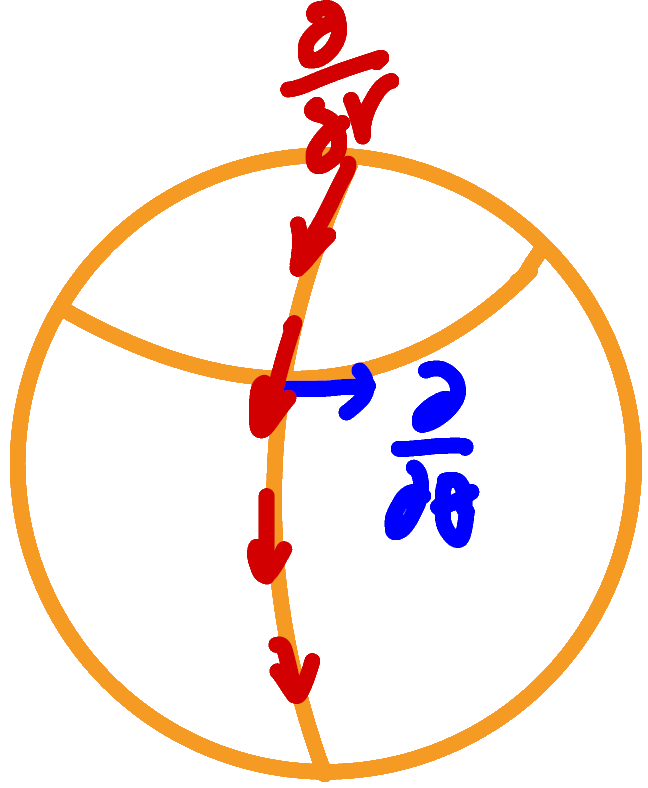
\includegraphics[scale=.2]{picture/week11/coordinate on S2.png}
    \end{center}
    Fixing \(\theta\), then \(\pdv{r}\) is the tangent vector field
    of the great circle, then 
    \[
        \frac{D}{dr}\left(\pdv{r}\right)=\nabla_{\pdv{r}}\pdv{r}
        =\Gamma\indices*{_{rr}^r}\pdv{r}+\Gamma\indices*{_{rr}^\theta}
        \pdv{\theta},
    \]
    where
    \[
        \Gamma\indices*{_{rr}^r}=\frac{1}{2}g^{rk}\left(
            \pdv{g_{rk}}{r}+\pdv{g_{rk}}{r}-\pdv{g_{rr}}{x^k}
        \right)
        =\frac{1}{2}g^{rr}\pdv{g_{rr}}{r}=0.
    \]
    \[
        \Gamma\indices*{_{rr}^\theta}=\frac{1}{2}
        g^{\theta\theta}\left(
            \pdv{g_{r\theta}}{r}
            +\pdv{g_{r\theta}}{r}
            -\pdv{g_{rr}}{\theta}
        \right)
        =0    
    \]
    \(\Rightarrow\frac{D}{dr}\pdv{r}=0\Rightarrow\) \(\pdv{r}\)
    is parallel along itself.

    If we compute 
    \[
        \frac{D}{d\theta}\pdv{\theta}=\nabla_{\pdv{\theta}}\pdv{\theta}
        =\Gamma\indices*{_{\theta\theta}^r}\pdv{r}+\Gamma
        \indices*{_{\theta\theta}^\theta}\pdv{\theta}
        =-\sin r\cos r \pdv{r}.    
    \]
    Hence, 
    \[
        \textcolor{blue}{
            \frac{D}{d\theta}\pdv{\theta}=0
            \Longleftrightarrow r=\frac{\pi}{2}.}
    \]
\end{remark}
\underline{Facts}:
\[
    \frac{DV(t)}{dt}=0\Longleftrightarrow 
    \dot{V}^i(t)+\Gamma\indices*{_{jk}^i}(t)\dot{x}^j(t)V^k(t)=0.    
\]
This is the \engordnumber{1} order linear O.D.E. system of
\(V(t)\). Hence, given a curve \(\alpha(t)\), let \(p\in\alpha(t)\),
\(v_0\in T_p M\), then by the Solution to the Cauchy problem, there is 
a unique parallel vector field \(V(t)\) along \(\alpha(t)\) such that 
\(V(0)=v_0\). 
\begin{center}
    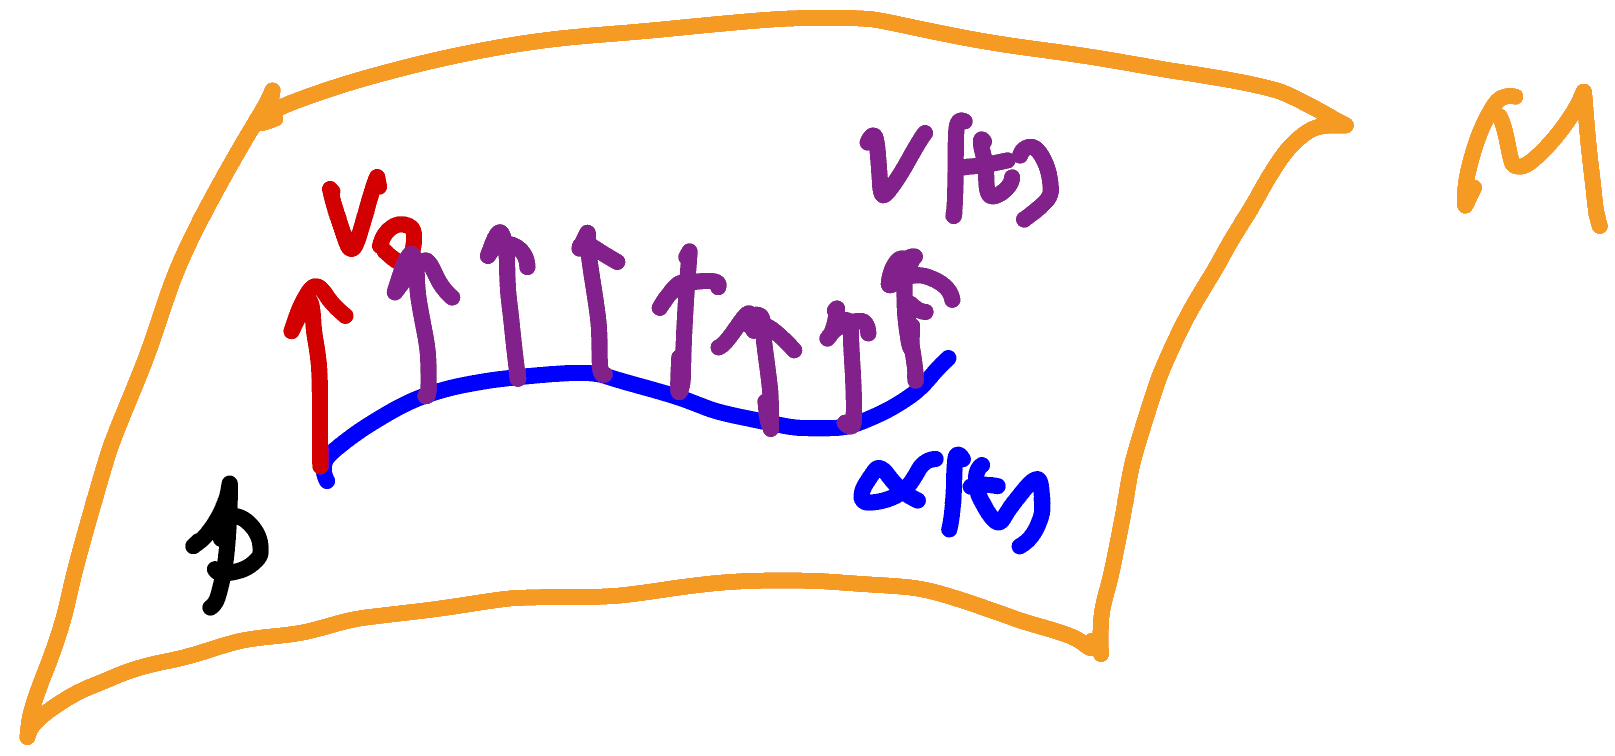
\includegraphics[scale=0.25]{picture/week11/parallel transport.png}
\end{center}
Consider \(p,q\in M\), let \(\alpha(t)\colon[0,1]\to M\) such that 
\(\alpha(0)=p,\alpha(1)=q,v_0\in T_p M\), and \(V(t)\) is the parallel 
vector field along \(\alpha(t)\) with \(V(0)=v_0\), then 
\textcolor{blue}{
    \(V(1)\in T_q M\) is called the parallel transportation of 
    \(v_0\) at \(q\).
}
\textcolor{blue}{
    \begin{proposition}
        Let \(V_1,V_2\) be two parallel vector fields along a curve 
        \(\alpha(t)\), then \(\left\langle V_1,V_2 \right\rangle\)
        is a constant along \(\alpha(t)\).
    \end{proposition}
}
\begin{proof}
    \(\dv{t}\left\langle V_1(t),V_2(t)\right\rangle
    =\left\langle\dv{V_1(t)}{t},V_2(t)\right\rangle
    +\left\langle\dv{V_2(t)}{t},V_1(t)\right\rangle
    =0\).
\end{proof}
\textcolor{blue}{
    \begin{corollary}
        The parallel transport along a curve does not
        change the length or angle of original vectors.
        \begin{center}
            \includegraphics[scale=0.2]{picture/week11/p. transport 
            isometry.png}
        \end{center}
        In particular, the map 
        \[  
            P_{\alpha(1)}\colon T_p M\to T_q M
        \]
        is a linear isometry.
    \end{corollary}
}
\begin{remark}
    The advantage of parallel transport is helping us choose an
    orthonormal frame along a curve \(\alpha(t)\). At \(T_p M\),
    choose orthonormal basis \{\(E_1,\ldots,E_n\)\} and parallel
    transport \(E_i\) along \(\alpha\), then at each point 
    of the curve \(\{E_1(t),\ldots,E_n(t)\}\)is an orthonormal basis
    of \(T_{\alpha(t)}M\).
    \begin{center}
        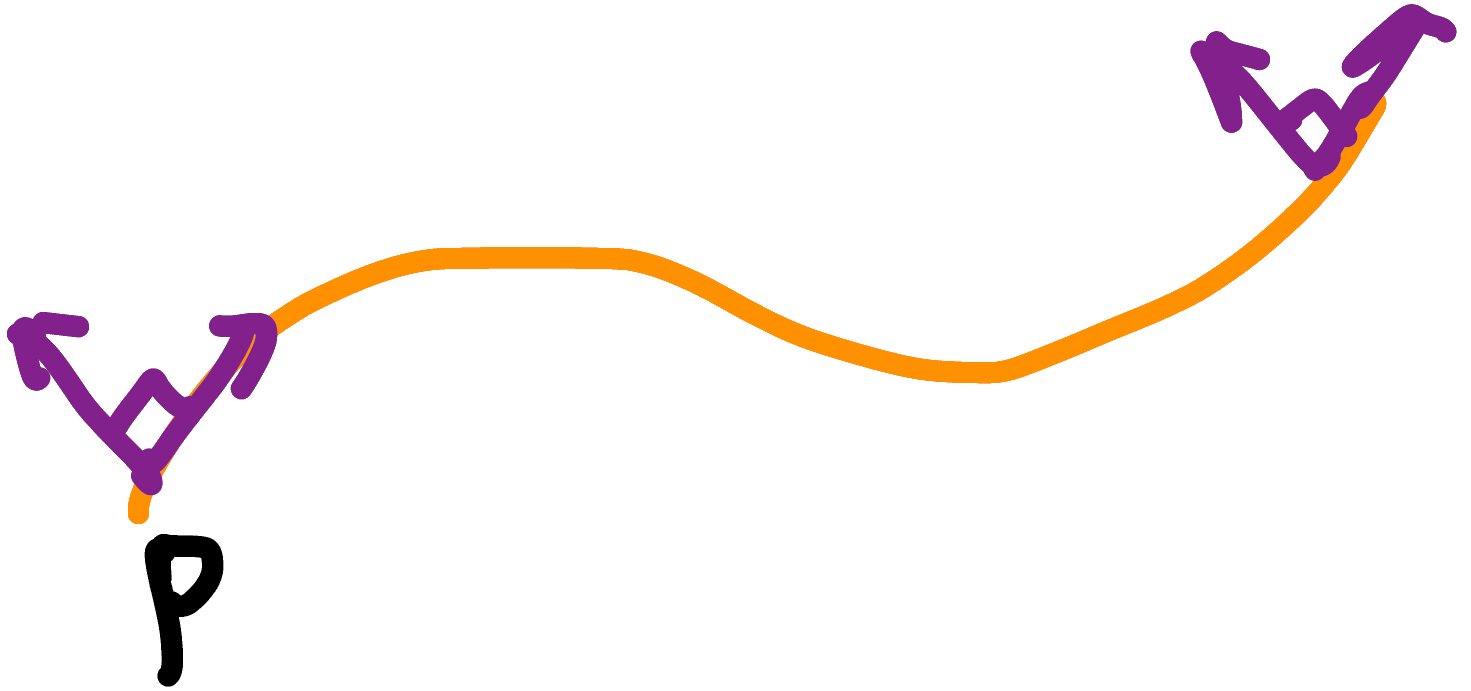
\includegraphics[scale=0.15]{picture/week11/orthonormal basis.png}
    \end{center}
    For any vector field \(V(t)\) along
    \(\alpha(t)\), \textcolor{blue}{\(V(t)=V^i(t)E_i(t)\)},
    \[
        \frac{DV(t)}{dt}=\frac{D}{dt}\left(
            V^i(t)E_i(t)
        \right)    
        =\dot{V}^i(t)E_i(t)+V^i(t)\underbrace{\frac{DE_i(t)}{dt}}_{=0}.
    \]
    \[
        \frac{DV(t)}{dt}=\dot{V}^i(t)E_i(t).
    \]
\end{remark}
\begin{remark}
    \(\forall p\in M\), let \(\alpha\) be a piecewise 
    smooth \textcolor{blue}{closed} curve  passing through \(p\),
    then the parallel transport \(P_\alpha\colon T_p M\to T_p M\)
    yields a linear isometry of \(T_p M\). If \(\beta\) is another
    piecewise \textcolor{blue}{closed} curve passing through \(p\),
    we have another linear isometry \(P_\beta\).
\end{remark}
\textcolor{blue}{
    \begin{definition}
        \[\mathrm{Hol}_p(M,g)=\{P_\alpha\colon T_p M\to T_p M,
        \alpha\text{: closed curve passing
        through }p\}.\]
        \begin{center}
            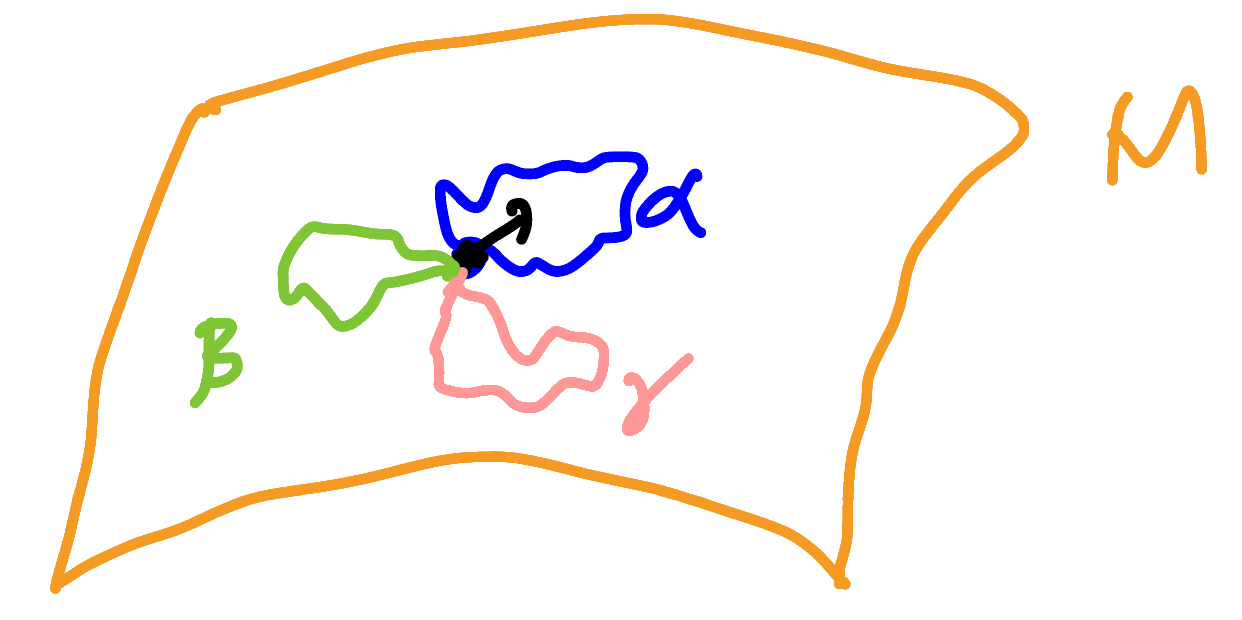
\includegraphics[scale=0.3]{picture/week11/holonomy groups.png}
        \end{center}
    \end{definition}
}
This set has a group structure given by composition of parallel transport.
\(\mathrm{Hol}_p(M,g)\) is called the Holonomy group of \(M\) at \(p\).
In fact, it's a Lie group. Note that \(\mathrm{Hol}(M,g)\) relies on 
the Riemannian metric \(g\).\

\textcolor{cyan}{
    {\Large \textbf{!}} The classification of Holonomy group is useful 
    to understand the classification of Riemannian manifold (metric). 
    Details can be found in Peter Perterson's Riemannian Geometry
    book p.388.
}
\textcolor{blue}{
    \begin{definition}[Geodesics]
        \(\gamma(t)\) is a parametrized curve in \(M\), if
        \[
            \frac{D}{dt}\dot{\gamma}(t)=0\left(\Longleftrightarrow
            \nabla_{\dot{\gamma}(t)}\dot{\gamma}(t)=0
            \text{ or simply }\nabla_{\dot{\gamma}}\dot{\gamma}\right).    
        \]
        \ie\ \(\dot{\gamma}(t)\) is a parallel vector field along
        \(\gamma(t)\), then we call \(\alpha(t)\) a geodesic. 
    \end{definition}
}
\begin{remark}
    By definition, \(\left\langle\dot{\gamma}(t),\dot{\gamma}(t)
    \right\rangle\) is constant, after reparametrization,
    \(\gamma(t)=\gamma(s),s=ct\) is the arclength parameter,
    \(\therefore\) a curve \(\alpha(s)\) with arclength parameter
    is a geodesic iff \(\frac{D}{ds}\left(\alpha'(s)\right)=0\).
\end{remark}
\subsection{Geodesics on surfaces}
Let \(S\) be a regular surface in \(\mathbb{R}^3\). Let \(\alpha(s)\)
be a geodesic on \(S\) with arclength parameter. Then \(\alpha''(s)\)
(in \(\mathbb{R}^3\)) has the following decomposition
\begin{align*}
    \alpha''(s)&=\frac{D}{ds}\left(\alpha'(s)\right)+
    \left\langle\alpha''(s),\va*{N}\left(\alpha(s)\right)\right\rangle
    \va*{N}\\
    &=\left\langle\alpha''(s),\va*{N}\left(\alpha(s)\right)\right\rangle
    \va*{N}\\
    &=k_{\vb{n}}(s)\va*{N}.\footnotemark
\end{align*}
\footnotetext{Recall that \(k_{\vb{n}}(s)=\II \left(\alpha'(s),
\alpha'(s)\right)\).}
\(\therefore \alpha(s)\) is a geodesic \(\Longleftrightarrow\) principal
normal \(\va{n}(s)\) is parallel to the normal of surface \(\va*{N}\).
Note normal section is a geodesic, but geodesic may not be a normal
section.
\begin{enumerate}[(1)]
    \item \(\mathbb{S}^2\). Great circles are geodesics.
    \begin{center}
            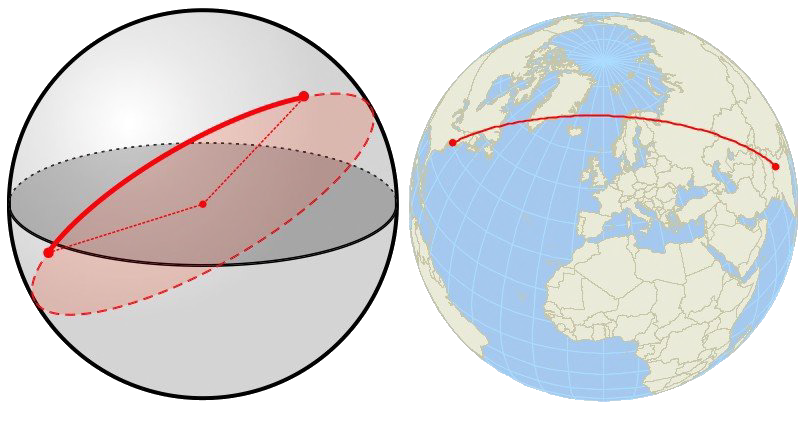
\includegraphics[scale=0.7]{picture/week11/geodesics on S2.png}
    \end{center}
    \item On Cylinder, \(x^2+y^2=1\), 
    \begin{center}
        \includegraphics[scale=0.5]{picture/week11/geodesics on 
        cylinder.png}
    \end{center}
    consider the local parametrization
    \[\gamma(u,v)=\left(\cos u ,\sin u,v\right)\]
    \(\Rightarrow\) lines, horizontal circles, and helix curve
    \(\left(\cos as,\sin as, bs\right)\) are all geodesics.
\end{enumerate}

\subsection{Geodesic curvature}
Let \(\alpha(s)\colon I\to S\) be a regular curve, at each point \(p\in \alpha\).
We have two o.n. frames:
\begin{enumerate}[(1)]
    \item Frenet's formula \(\{\vec{t}(s),\vec{n}(s),\vec{b}(s)\}\);
    \item \(\{\vec t(s),N(s)\times \vec t(s),N(s)\}\), \(N(s)\) is unit normal of
        \(S\) at \(\alpha(s)\).
\end{enumerate}
Using the second frame, we have \[
    \left<\alpha''(s),N(s)\right> =\II(\alpha'(s),\alpha'(s))=k_n,
    \text{ normal curvature at }\alpha(s)
.\] 

\begin{definition}[Geodesic curvature]
    \[
        k_g:=\left<\alpha''(s),N(s)\times \vec t(s)\right> 
    \] is called geodesic curvature.
\end{definition}

By the Frenet formula, \(\alpha''(s)=\vec t'(s)=k\vec n(s)\), let \(\theta\) be the
angle between \(\vec n(s)\) and \(N(s)\), then
\begin{align}
    k_n&= k\cos\theta=\left<\alpha''(s),N(s)\right> &\text{normal curvature} \\
    k_g&= \pm k\sin\theta=\left<\alpha''(s),\right> &\text{geodesic curvature}
.\end{align}
The sign of expression of \(k_g\) depends on the choice of normal of surface
and orientation of \(\alpha(s)\).

Hence \[
    k^2=k_n^2+k_g^2
.\] And \(\alpha(s)\) is geodesic \(\iff \vec n\parallel N\iff k_n=k\iff k_g=0\).

\begin{exercise}[Liouvill formula]
    Let \(\vphi(u,v)\) be an orthogonal parametrization of a regular surface \(S\),
    \(\alpha(s)\) be a regular curve on \(S\) with arclength parameter.
    Let \(\theta(s)\) be the angle between \(u\)-curve and \(\alpha'(s)\). Then \[
        k_g=\dv{\theta}{s}-\frac{1}{2\sqrt{G}}\pdv{\log E}{v}\cos\theta
        +\frac{1}{2\sqrt{E}}\pdv{\log G}{u}\sin\theta
    .\] 
\end{exercise}

\subsection{Length minimizing curves (variational viewpoint)}
\((M,g)\) be Riemannian manifold, let \(\gamma(s)\colon [0,l]\to M\) be a curve
with arc-length parameter. \(\gamma(0)=:p,\gamma(l)=:q\). Let \(\Gamma(s,t)\) be a
family of smooth variation with endpoints fixed.
\ie\ \(\Gamma(s,t)\colon [0,l]\times (-\eps,\eps)\to M\) \st\ \(\forall\,t\in (-\eps,
\eps)\), \(\Gamma(s,t_0)\) is a \(C^\infty\) curve with initial point \(p\) and
endpoint \(q\), and, \(\Gamma(s,0)=\gamma(s)\).

Consider the arc-length functional \[
    L(\Gamma(s,t))=\int_{0}^{l}\left|\pdv{\Gamma(s,t)}{s}\right|\dd{s}
.\] 
Then
\begin{equation}\label{eq:variation-geodesic}
\begin{split}
    \eval{\dv{t}}_{t=0}L(\Gamma(s,t))
    &=\int_{0}^{l}\frac{1}{2}\left<\dot\gamma(s),\dot\gamma(s)\right> ^{-\frac{1}{2}}
    \eval{\dv{t}}_{t=0}\left<\dv{\Gamma(s,t)}{s},\dv{\Gamma(s,t)}{s}\right> \dd{s} \\
    &=\int_{0}^{l}\left<\eval{\frac{\mathrm{D}}{\dd{t}}}_{t=0}
    \left(\pdv{\Gamma(s,t)}{s}\right),\dot\gamma(s)\right> \dd{s}.
\end{split}
\end{equation}

\begin{lemma}
    \[
        \frac{\mathrm{D}}{\dd{t}}\left( \pdv{\Gamma(s,t)}{s} \right) 
        =\frac{\mathrm{D}}{\dd{s}}\left(\pdv{\Gamma(s,t)}{t}\right)
    .\] 
\end{lemma}
\begin{proof}
Let \((x^1,\ldots,x^n)\) be local coordinate \st\ \(\Gamma(s,t)\) is contained
in this coordinate chart.
\begin{flalign*}
    \implies &\Gamma(s,t)=(x^1(s,t),\ldots,x^n(s,t))
    \implies \begin{cases}
        \pdv{\Gamma}{s}=x^i_s\pdv{x^i} \\
        \pdv{\Gamma}{t}=x^i_t\pdv{x^i}
    \end{cases}. &
\end{flalign*}
\begin{flalign*}
    \implies \frac{\mathrm{D}}{\dd{t}}\left(\pdv{\Gamma}{s}\right)
    &=\frac{\mathrm{D}}{\dd{t}}\left(x^i_s\pdv{x^i}\right) & \\
    &=x^i_{st}\pdv{x^i}+x^i_s x^j_t\nabla_{\pdv{x^i}}\pdv{x^j} \\
    &=\frac{\mathrm{D}}{\dd{s}}\left(\pdv{\Gamma}{t}\right)
.\end{flalign*}
\end{proof}

Then
\begin{flalign*}
    \text{\cref{eq:variation-geodesic}}
    &= \int_{0}^{l}\left<\frac{\mathrm{D}}{\dd{s}}\left(\eval{\pdv{\Gamma}{t}}_{t=0}
    \right),\dot\gamma(s)\right> \dd{s} & \\
    &= \eval{\left<\eval{\pdv{\Gamma}{t}}_{t=0},\dot\gamma(s)\right>}_0^l
    -\int_{0}^{l}\left<\eval{\pdv{\Gamma}{t}}_{t=0},\nabla_{\dot\gamma}
    \dot\gamma\right> \dd{s}
.\end{flalign*}
Note the variational family fix endpoints.
\begin{flalign*}
    \implies & \eval{\pdv{\Gamma}{t}}_{t=0}=\eval{\pdv{\Gamma}{t}}_{t=0}(l)=0 &
\end{flalign*}
Hence
\begin{flalign*}
    \text{\cref{eq:variation-geodesic}}
    &=-\int_{0}^{l}\left<\eval{\pdv{\Gamma}{t}}_{t=0},\nabla_{\dot\gamma}\dot\gamma
    \right> \dd{s} &
\end{flalign*}
Hence Euler-Lagrange equation is \(\nabla_{\dot\gamma}\dot\gamma=0\) (geodesic
equation).

We conclude that if \(\gamma(s)\) is a curve having shortest length between two points
on \(M\), then it must be a geodesic. Conversely, we only have geodesics are local
minimizing curves (prove later).

\begin{example}
    Every great circle on \(\mathbb{S}^2\) is a geodesic.
\end{example}
Note \[
    \nabla_{\dot\gamma}\dot\gamma=0\iff \ddot x^k(t)+\Gamma_{ij}^k(x(t))\dot x^i(t)
    \dot x^j(t)=0.
\] By ODE theory, at each point \(p=(x^1(t_0),\ldots,x^n(t_0))\) with any prescribed
direction \(v=\dot x^k(t_0)\pdv{x^k}\), there is a unique geodesic starting at \(p\)
with initial velocity \(v\). Locally, \ie\ \(\exists\,\gamma(t)\colon (0,\eps)\to M\)
geodesic \st\ \(\gamma(0)=p,\dot\gamma(0)=v\).

\begin{remark}
\begin{enumerate}[(1)]
\item Previously, we have considered the length functional of a family of curves
    \(\Gamma(s,t)=\gamma_t(s)\colon [0,l]\to M\): \[
        L(\gamma_t(s))=\int_{0}^{l}\left|\dot\gamma_t(s)\right|\dd{s}
    .\] In fact, when we consider the Euler-Lagrange equation, it's more convenient
    to consider the ``energy'' functional 
    \begin{equation}\label{eq:energy-functional}
        E(\gamma_t(s))=\frac{1}{2}\int_{0}^{l}\left|\dot\gamma_t(s)\right|^2\dd{s}
    .\end{equation}
    (Then there won't appear denominator term).
\item A generalization of such type of functional: let \(u\colon(M,g)\to (N,h)\)
    be \(C^\infty\) map, the energy functional is \[
        E(u)=\int_{M}\left|\dd{u}\right|^2\dd{V_g}
    .\] If \((x^1,\ldots,x^m)\) is local coordinate of \(M\), \(u(x)=(u^1,\ldots,u^n)
    \), then \[
        \left|\dd{f}\right|_{g,h}^2=g^{ij}h_{\alpha\beta}
        \pdv{u^\alpha}{x^i}\pdv{u^\beta}{x^j}
    .\] As special cases:
    \begin{enumerate}[(a)]
    \item If \(M\) is an interval \([a,b]\), \(u\colon [a,b]\to (N,h)\), \(E(u)\)
        is just~\cref{eq:energy-functional}.
    \item If \(M=\Omega\subset \mathbb{R}^n,N=\mathbb{R}\), \ie\ \(u\) is smooth
        function \(\Omega\to \mathbb{R}\) with compact support, \[
            E(u)=\int_{\mathbb{R}^n}|\dd{f}|^2\dd{x^1}\cdots \dd{x^n}
        .\] Then Euler-Lagrange equation is just harmonic function equation.
    \end{enumerate}
\end{enumerate}
\end{remark}

\begin{definition}
    The solution of Euler-Lagrange equation of~\cref{eq:energy-functional} is called
    harmonic maps.
\end{definition}

\subsection{Complete manifold}
From geodesic equation \(\nabla_{\dot\gamma}\dot\gamma=0\), \(\forall\,p\in M,v\in
T_p M\), \(\exists\) unique geodesic \(\gamma(t)\colon (-\eps,\eps)\to M\) \st\ 
\(\gamma(0)=p,\dot\gamma(0)=v\). In fact we can write \(\gamma(t)=\exp_p(tv)\) locally.

A natural question to ask in how large the defining domain of \(\gamma(t)\) could be.

\noindent{\large\color{blue}\boxed{Observation}} If \(I_1,I_2\) are two interval in
\(\mathbb{R}, t_0\in I_1\cap I_2\), \(\gamma_1\colon I_1\to M,\gamma_2\colon I_2\to M\)
are two geodesics \st\ \(\gamma_1(t_0)=\gamma_2(t_0)\) and \(\dot\gamma_1(t_0)
=\dot\gamma_2(t_0)\). Then \(\gamma_1\) and \(\gamma_2\) agree on \(I_1\cap I_2\) by
uniqueness of solution of ODE\@.

Then \(\gamma_1\cup \gamma_2\) is an extension of geodesics \(\gamma_1\) and
\(\gamma_2\). Furthermore, it is also a geodesic defined on \(I_1\cup I_2\).

\begin{definition}[Maximal geodesic]\hfill\\
    \(\gamma(t)\colon I\to M\) is called a maximal geodesic if \(I\) is the largest
    defining domain of \(\gamma(t)\), \ie\ it cannot be extended to a geodesic on
    a larger interval containing \(I\).
\end{definition}
\begin{remark}
    A maximal geodesic can be defined on
    \begin{enumerate}[(1)]
    \item \(\mathbb{R}\);
    \item Finite open interval \((a,b)\);
    \item Half interval \((-\infty,b)\) or \((a,+\infty)\).
    \end{enumerate}
\end{remark}
\begin{definition}[Complete manifold]\hfill\\
    A Riemannian manifold \((M,g)\) is called (geodesic) complete if all maximal
    geodesics are define on \(\mathbb{R}\).
\end{definition}
\begin{remark}
    This means each geodesic starting from a point \(p\) with initial velocity \(v\)
    can be extended from both sides for all time. Furthermore, \(\exp_p\colon
    T_p M\to M\) is defined for all \(v\in T_p M\).
\end{remark}

\begin{example}
    \(\mathbb{R}^2\setminus\{0\}\) is not geodesic complete. Consider geodesic
    \(\gamma(t)=(t,0)\), which can only be defined on \((-\infty,0)\).
\end{example}

For the completeness of a manifold, we mention the Hopf-Rinow theorem, the proof of
which will be left to Riemannian geometry course.

Note the Riemannian metric \(g\) on \(M\) defines a distance function \[
    d(p,q)=\inf\{L(\gamma):\gamma\text{ piecewise smooth from } p \text{ to }q\}
.\] Then \(M\) became a metric space.

Recall a metric space \((M,d)\) is complete if every Cauchy sequence is convergent.

\begin{theorem}[Hopf-Rinow]\label{thm:hopf-rinow}
    Let \((M,g)\) be a manifold without boundary, TFAE\@:
    \begin{enumerate}[(1)]
    \item \((M,g)\) is geodesic complete.
    \item \((M,g)\) is geodesic complete at some \(p\in M\), \ie\ \(\exp_p\) is defined
        on whole \(T_p M\).
    \item \((M,d)\) is complete metric space.
    \item \(A\subset M\) is compact iff \(A\) is bounded and closed.
    \item Every closed geodesic ball \(\overline{B}(p,r)\) is compact.
    \end{enumerate}
\end{theorem}

\begin{corollary}
    If \((M,g)\) is complete, then any \(p,q\in M\) can be jointed by a minimal
    geodesic, \ie\ the distance \(d(p,q)\) is realized by length of a geodesic.
\end{corollary}
\begin{corollary}
    If \((M,g)\) is closed manifold (compact without boundary), then \((M,g)\) is
    complete. In particular, any surface without boundary in \(\mathbb{R}^3\) which is
    a closed subset is complete.
\end{corollary}

\begin{remark}
    One of the famous incomplete Riemannian metric lies in the study of geometry of
    the moduli space (or Teichm\"uller space) of Riemann surfaces: \[
        T_g=\frac{\{\text{Conformal structure of }\Sigma_g\}}{\text{Orientation
        preserving diffeomorphisms}}
    .\] On \(T_g\), each point represents a Riemann surface of genus  \(g\) with a
    given conformal structure. There is a metric on such space defined by \(L^2\)
    pairing of infinitesimal conformal structure at each point. Such metric is called
    the Weil-Petersson metric an it's not complete.
\end{remark}

\noindent{\color{red}\underline{Key fact:}} Studying the metric completion of
Weil-Petersson metric is related to the compactification of the moduli space!
This is one of many correspondence of Differential Geometry \(\longleftrightarrow\)
Algebraic Geometry.

\subsection{Exponential map \& geodesic spherical coordinate}
Let's first see a rescaling argument of geodesic:

We have seen \(\forall\,p\in M\), along any prescribed velocity \(v\in T_p M\), there
is a unique geodesic \(\gamma(t)\colon [0,\eps)\to M\) \st\ \(\gamma(0)=p,
\dot\gamma(0)=v\). By rescaling the velocity \(v\rightsquigarrow\lambda v\), we obtain
the geodesic \(\beta(\tau)\colon[0,\frac{\eps}{\lambda})\to M\), which has the same
trace with \(\gamma(t)\) and \(\beta(0)=p,\dot\beta(0)=\lambda v\). In particular,
we introduce notation \[
    \gamma(t,v)=\gamma(t),\quad \beta(\tau,\lambda v)=\beta(\tau),\quad \lambda\tau=t
.\] Then \(\beta(\tau,\lambda v)=\beta(\tau)=\gamma(t)=\gamma(t,v)=\gamma(\lambda\tau,v
),\forall\,\tau\in [o,\frac{\eps}{\lambda})\).

This rescaling argument allows us to consider geodesics defined on \([0,1]\).
\begin{definition}[Exponential map]
    Let \(p\in M,v\in T_p M,\gamma\colon[0,1]\to M\) is a geodesic \st\ \(\gamma(0)=p,
    \gamma'(0)=v\). The exponential map is defined as
    \begin{align*}
        \exp_p\colon T_p M &\longrightarrow M \\
        v &\longmapsto \exp_p(v)=\gamma(1)
    .\end{align*}
\end{definition}
Note the length of \(\gamma\) between \(p\) and \(\gamma(1)\) is \(|v|\), and
\(\gamma(t)=\exp_p(tv)\) for \(t\in [0,1]\), \(\exp_p(0)=p\). Hence geodesic \(\gamma
(t)\) is the image of ray from \(0\) in \(T_p M\) under \(\exp_p\).

We state the following fact without proof:
\begin{prop}
    \(\exists\,\eps>0\) \st\ \(\exp_p\colon B(0,\eps)\to M\) is a diffeomorphism
    where \(B(0,\eps)\) is ball of radius \(\eps\) centered at origin in \(T_p M\).
\end{prop}
\begin{remark}
    The radius \(\eps\) could be very large or even \(\infty\), but also could be
    a finite number.
\end{remark}

\begin{example}
    \(\exp_p\colon T_p M\to M\) where \(p\) is north pole in \(\mathbb{S}^2\).
    \(\exp_p(v)=q\) the south pole if \(|v|=\pi\), then \(\exp_p\) fails to be a
    diffeomorphism on \(B(0,r),r>\pi\).
\end{example}

\begin{definition}
    \(W\subset M\) is called a normal neighbourhood of \(p\), if for some \(U\subset 
    T_p M\) containing 0, \(\exp_p\colon U\to W\) is diffeomorphism.
\end{definition}

For normal neighbourhood, we can endow coordinate at \(p\) by considering the image
of Cartesian coordinate and polar coordinate at origin of \(T_p M\cong \mathbb{R}^n\).

\subsubsection*{Normal coordinate}
Let \(e_1,\ldots,e_n\) be orthonormal basis of \(T_p M\cong \mathbb{R}^n\), for any
vector \(v\in U\subset T_p M\), write \(v=x^i e_i\).
Then we say \(q=\exp_p(v)\) has coordinate \((x^1,\ldots,x^n)\). In particular,
\(\exp_p(tv)\) has coordinate \((tx^1,\ldots,tx^n)\) and \(p\) has coordinate \(0\).

Since \(\gamma(t)=\exp_p(tv)\) satisfies geodesic equation, it writes: \[
    \gamma^k(t)=tx^k,\ \Gamma_{ij}^k(\gamma(t))x^i x^j=0\quad
    (\ddot \gamma^k(t)+\Gamma_{ij}^k(\gamma(t))\dot x^i(t)\dot x^j(t)=0)
.\] At \(p=\gamma(0)\), \(\Gamma_{ij}^k(\gamma(0))x^i x^j=0\). Since \(v=x^i e_i\) is
chosen arbitrarily, we conclude that \(\Gamma_{ij}^k=0\) at \(p\).
Moreover, \(g_{ij}(p)=g(e_i,e_j)=\delta_{ij}\).

We summarize that the normal coordinate \((x^1,\ldots,x^n)\) in a neighbourhood of 
\(p\) has the following properties:
\begin{enumerate}[(1)]
\item \(p=(0,\ldots,0)\) ;
\item \(g_{ij}(p)=\delta_{ij}\) ;
\item \(\Gamma_{ij}^k(p)=0\);
\item \(\tensor{R}{_{ij}^k_l}(p)=(\pdv{x^i}\Gamma_{jl}^k-\pdv{x^j}\Gamma_{il}^k)(p)\);
\item \(\triangle_g f(p)=g^{ij}(\partial_i \partial_j f-\Gamma_{ij}^k \partial_k f)(p)
    =\triangle f(p)\).
\end{enumerate}

\subsubsection*{Geodesic spherical coordinate}
Take \((\rho,\theta^1,\ldots,\theta^{n-1})\) as polar coordinate in \(T_p M\cong 
\mathbb{R}^n\). Let \(U\) be normal neighbourhood of \(p\in M\). Then \\
Geodesic sphere \(=\) image of \(\{r=r_0\}\) under \(\exp_p\); \\
Radial geodesic \(=\) image of \(\{\theta=\theta_0\}\) under \(\exp_p\).

\((\rho,\theta^1,\ldots,\theta^{n-1})\) is called the geodesic spherical coordinate
and the vector fields are \(\pdv{\rho},\pdv{\theta^1},\ldots,\pdv{\theta^{n-1}}\).

Note \(\theta=\theta_0\) is a ``straight ray'' and \(\rho\) is just the arc-length
parameter of radial geodesic. Hence in \((\rho,\theta^1,\theta^{n-1})\) coordinate
the coefficient of the Riemannian metric. \[
    g_{11}=g(\pdv{\rho},\pdv{\rho})=1\iff \pdv{\rho}\text{ is a radial unit vector
    filed}
.\] Next we study \(g_{\rho\theta^i}\), we'll show it's 0. Let's argue for surface
since \(\theta=\theta_0\) is geodesic, 
\begin{flalign*}
    \implies & \nabla_{\pdv{\rho}}\pdv{\rho}=0
    \implies \Gamma_{11}^1\pdv{\rho}+\Gamma_{11}^2\pdv{\theta}=0. & \\
    \implies & \Gamma_{11}^1=0, \Gamma_{11}^2=0 \\
    & 0=\Gamma_{11}^1=g^{12}\partial_1 g_{12}=-\frac{1}{\det g}g_{12}\partial_1 g_{12}
.\end{flalign*}
Since \(g^{22}=\frac{1}{\det g}g^{11}\neq 0\), \(\partial_1 g_{12}=0\), \ie\ \(g_{12}\)
is independent of \(\rho\).

Note that \((x_1,x_2)=(\rho\cos\theta,\rho\sin\theta)\), \[
    g_{12}=g(\pdv{\rho},\pdv{\theta})=g(\cos\theta\pdv{x^1}+\sin\theta\pdv{x^2},
    -\rho\sin\theta\pdv{x^1}+\rho\cos\theta\pdv{x^2})
.\] Hence \(g_{12}(\rho,\theta)=\lim_{\rho \to 0} g_{12}(\rho,\theta)=0\).

\begin{exercise}
    Proof \(g_{\rho\theta^i}=0\) for general case.
\end{exercise}

We summarize: In geodesic polar coordinate \((\rho,\theta^1,\ldots,\theta^{n-1})\),
\begin{enumerate}[(1)]
\item \(\pdv{\rho}\) is a unit vector field generating a radical geodesic;
\item \(\pdv{\rho}\perp \pdv{\theta}\), \ie\ radial geodesic is orthogonal to
    geodesic spheres.
\end{enumerate}
These two results are called the \emph{Gauss Lemma}.

Hence in geodesic polar coordinate, the metric is \[
    \dd{s}^2=\dd{\rho}^2+\tilde{g}_{ij}(\rho,\theta)\dd{\theta^i}\dd{\theta^j}
.\] 

\begin{exercise}
    If \(S\) is a surface, \((\rho,\theta)\) is geodesic polar coordinate, show that \[
        \lim_{\rho \to 0} \sqrt{G}=0,\quad
        \lim_{\rho \to 0} (\sqrt{G})_\rho=1
    .\] 
\end{exercise}
\begin{remark}
    In surface case, the Gaussian curvature has expression \[
        K=-\frac{(\sqrt{G})_{\rho\rho}}{\sqrt{G}}
        =-\pdv[2]{\rho}(\log \sqrt{G})
        -(\pdv{\rho}\log\sqrt{G})^2
    .\] 
\end{remark}

{\color{red}
So far, we have seen two useful local expression of Gaussian curvature:
\begin{enumerate}[(1)]
\item \(\dd{s}^2=\dd{r}^2+G(r,\theta)\dd{\theta}^2\implies 
    K=-\frac{(\sqrt{G})_{rr}}{\sqrt{G}}\);
\item \(\dd{s}^2=\lambda(u,v)(\dd{u}^2+\dd{v}^2)
    \implies K=-\frac{1}{2\lambda}\triangle \log\lambda\).
\end{enumerate}
}

\noindent\underline{\bfseries Recall:}
\begin{itemize}
\item \(\mathbb{R}^2\): \(\dd{s^2}=\dd{r^2}+r^2\dd{\theta}^2\implies K=0\).
\item \(\mathbb{S}^2\): \(\dd{s^2}=\dd{r^2}+\sin^2 r\dd{\theta}^2\implies K=1\).
\item \(\mathbb{H}^2\): \(\dd{s^2}=\dd{r^2}+\sinh^2 r\dd{\theta}^2\implies K=-1\).
\end{itemize}
Conversely, if we prescribe the Gaussian curvature \(K=0,\pm1\), then solving
ODE \[
    \begin{cases}
        (\sqrt{G})_{rr}+K\sqrt{G}=0, \\
        \lim_{r\to 0}\sqrt{G}=0,\ \lim_{r\to 0}(\sqrt{G})_r=1
    \end{cases}
.\] Hence, \(\dd{s}^2\) can be written in standard form above. This implies if two
regular surfaces have the same constant Gaussian curvature, they must be locally
isometric. This is \emph{Minding's theorem}.

\subsection{Applications of Geodesic Polar Coordinate}

Recall previously, by comparing the area \(A\) of a small neighbourhood of \(p\in S\)
and the Area \(\overline{A}\) of its Gaussian image, then \[
    |K(p)|=\lim_{A \to 0} \frac{\overline{A}}{A}
.\] We also mentioned two more results:
\begin{enumerate}[I.]
\item Let \(C(r)\) be the image of circle of radius \(r\) centered at 0 in \(T_p S\)
    under exponential map, \ie\ the geodesic circle of radius \(r\), then \[
        K(p)=\lim_{r \to 0} 3\cdot\frac{2\pi r-L(C(r))}{\pi r^3}
    .\]
\item Consider similarly the geodesic disk \(D(r)\), then \[
    K(p)=\lim_{r \to 0} 12\cdot \frac{\pi r^2-A(D(r))}{\pi r^4}
.\]
\end{enumerate}
The proof of I and II both rely on the Taylor's expansion of metric tensor.
\begin{proof}
I. \[
    L(C(r))=\lim_{\eps \to 0} \int_{\eps}^{2\pi-\eps}\sqrt{G}\dd{\theta}
\] Since we care abort \(r\to 0\), we use Taylor's expansion of \(\sqrt{G}\).

Recall that \(\eval{\sqrt{G}}_{r=0}=0,\eval{(\sqrt{G})_r}_{r=0}=1\) and \(K=
-\frac{(\sqrt{G})_{rr}}{\sqrt{G}}\). Hence \[
    (\sqrt{G})_{rr}+K\sqrt{G}=0
,\] and \(\eval{(\sqrt{G})_{rr}}_{r=0}=0\). Take one more derivative we have \[
    (\sqrt{G})_{rrr}+K_r\sqrt{G}+K(\sqrt{G})_{r}=0
.\] Let \(r=0\), we see \[
    K(p)=-\eval{(\sqrt{G})_{rrr}}_{r=0}
.\] Hence the expansion is 
\begin{equation}\label{eqn:geodesic-circle}
    \sqrt{G}(r,\theta)=r-\frac{r^3}{3!}K(p)+o(r^3)
.\end{equation}
Then \(L(C(r))=2\pi r-\frac{r^3}{3}\pi K(p)+o(r^3)\), this gives I.

II.\@Follows by integrating \cref{eqn:geodesic-circle} from \(r=0\) to \(R\). We get \[
    A(R)=\int_{0}^{R}L(C(r))\dd{r}=\pi R^2-\frac{R^4}{12}\pi K(p)+o(R^4)
.\] This gives II.
\end{proof}

\subsection{Geodesics are Locally Length Minimizing}
\(\forall\,p\in S\), take a normal neighbourhood \(U\) of \(p\). The metric in geodesic
polar coordinate is \[
    \dd{s}^2=\dd{r}^2+G(r,\theta)\dd{\theta}^2
.\] By shrinking \(U\), we further require \(U=\{\exp_p(v):v\in B(0,\eps)\subset
T_p S\}\). For any \(q=(r_0,\theta_0)\in U\), we have \(r_0<\eps\), consider all
piecewise smooth curve from \(p\) to \(q\) on \(S\). Let \(\gamma(t)\colon [0,t_0]
\to S\) be such a curve. First observe that if \(\gamma(t)\) is entirely contained
in \(U\), we can let \(\gamma(t)=(r(t),\theta(t))\), then \[
    \gamma'(t)=r'(t)\pdv{r}+\theta'(t)\pdv{\theta}
.\] This gives 
\begin{align*}
    L(\gamma(t))&=\int_{0}^{t_0}\left(|r'(t)|^2+|\theta'(t)|^2 G(r,\theta)\right)
    ^{\frac{1}{2}}\dd{t} \\
    &\ge \int_{0}^{t_0}|r'(t)|\dd{t}\ge \int_{0}^{t_0}r'(t)\dd{d}=r(t_0)=r_0
.\end{align*}
Equality holds iff \(\theta'(t)\equiv 0\). \ie\ \(\gamma\) is the radical ray, which
is the geodesic from \(p\) to \(q\), given by \[
    \gamma(t)=\exp_p(r(t)\pdv{r})
.\] If the curve is not entirely in \(U\), let \(t_1\) be the first time \(\gamma\)
meets the boundary. Then for any \(t_2<t_1\) we know the length of \(\eval{\gamma}_{
[0,t_2]}\) must be greater than the geodesic one, \ie\ \[
    L(\gamma|_{[0,t_2]})=\int_{0}^{t_2}|\gamma'(t)|\dd{t}\ge r(t_2)
.\] Let \(t_2\to t_1\) we see \(L(\gamma)\ge r(t_1)=\eps>r_0\).

We conclude that in \(U\), any piecewise smooth curve has greater length than
(radical) geodesic.

\begin{remark}
\begin{enumerate}[(1)]
\item By the Cauchy problem's solution to geodesic equation \[
    \begin{cases}
        \ddot{x}^k(t)+\Gamma_{ij}^k(t)\dot{x}^i(t)\dot{x}^j(t)=0 \\
        \gamma(0)=p,\ \dot\gamma(0)=v_0
    \end{cases}
.\] There is a unique geodesic starting at \(p\), with initial velocity \(v_0\). Hence
in this arguement, by shrinking \(U\) if necessary, we can see in \(U\), there is
unique minimizing geodesic from \(p\) to \(q\).
\item {\color{blue}Try to think about how large the normal neighbourhood could be.}

    This will be answered after we study the second variation of arc-length 
    and this problem is related to the global geometry of the surface.
\item It's important to study the behavior of a family of geodesics from a point.
    The local picture should be kept in mind is:

    {\color{orange}``The smaller curvature is, the faster geodesics will separate''}
\end{enumerate}
\end{remark}


\section{Quick introduction to tensor and tensor field}
\begin{enumerate}[(I)]
    \item Let \(V\) be a vector space, \(\dim V=n\).
    \(V^*\) be the covector space=\{all linear functionals 
    \(\alpha\colon V\to \mathbb{R}\)\}. The pairing is given by 
    \[V^*\times V\to \mathbb{R}\]
    \[(\alpha,v)\mapsto \alpha(v)\]
    \begin{itemize}
        \item A \textcolor{blue}{covariant \(l\)-tensor} on \(V\)
        is a multilinear map 
        \textcolor{blue}{
            \[
                \omega\colon V\times \ldots \times V\to \mathbb{R}.
                \tag{1}    
            \]
        }
        A \textcolor{blue}{
            contravariant \(k\)-tensor 
        }
        is a multilinear map 
        \textcolor{blue}{
            \[
                X\colon V^*\times \ldots \times V^*\to \mathbb{R}.
                \tag{2}    
            \]
        }
        A \textcolor{blue}{
            tensor of \((k,l)\) type (\(k\)-contravariant, \(l\)-covariant)
        }
        is a multilinear map 
        \textcolor{blue}{
            \[
                T\colon  V^*\times \ldots \times V^*\times 
                V\times \ldots \times V \to \mathbb{R}.
                \tag{3}   
            \]
        }
        Let 
        \begin{center}
            \(
            \bigotimes^l V^*=\{\text{all covariant }l\text{-tensors}\}
            \Rightarrow \omega \text{ in (1) }\in \bigotimes^l V^*    
        \)

        \(
            \bigotimes^k V=\{\text{all contravariant }k\text{-tensors}\}
            \Rightarrow X \text{ in (2) }\in \bigotimes^k V    
        \)

        \(
            \mathcal{T}^{(k,l)}(V)=\{\text{all }(k,l)\text{-type tensors}\}
            \Rightarrow T\in \mathcal{T}^{(k,l)}(V)    
        \)
        \end{center}
        \item Next we talk about the \textcolor{blue}{tensor product}.
        Let \(T\in \mathcal{T}^{(k,l)}(V)\),
        \(S\in \mathcal{T}^{(p,q)}(V)\), then \(T\otimes S \in 
        \mathcal{T}^{(k+p,l+q)}(V)\) is defined as
        \textcolor{blue}{
            \begin{align*}
                &T\otimes S\left(\omega^1,\ldots,\omega^{k+p}
                ;X_1,\ldots, X_{l+q}\right)\\
                =&
                T\left(\omega^1,\ldots,\omega^{k}
                ;X_1,\ldots, X_{l}\right)
                S\left(\omega^{k+1},\ldots,\omega^{k+p}
                ;X_{l+1},\ldots, X_{l+q}\right) .
            \end{align*}
        } 
Let \(V=\Span\{E_1,\ldots,E_n\}\),
\(V^*=\Span\{\alpha^1,\ldots, \alpha^n\}\) with 
\(\alpha^i (E_j)=\delta^i_j\), or equivalently
\(E_j(\alpha^i)=\delta^i_j\). 

Then 
\[(1)\Rightarrow \omega=\omega_{i_1,i_2,\ldots,i_l} \alpha^{i_1}
\otimes \ldots \otimes \alpha^{i_l}.\]
Moreover, \begin{align*}
    \omega\left(E_{j_1},\ldots,E_{j_l}\right)
    &= \omega_{i_1,i_2,\ldots,i_l} \alpha^{i_1}
    \otimes \ldots \otimes \alpha^{i_l}\left(
        E_{j_1}\otimes \ldots\otimes E_{j_l}
    \right)\\
    &=\omega_{i_1,i_2,\ldots,i_l}
    \alpha^{i_1}(E_{j_1})\cdots \alpha^{i_l}(E_{j_l})\\
    &=\omega_{i_1,i_2,\ldots,i_l}\delta^{i_1}_{j_1}\cdots 
    \delta^{i_l}_{j_l}=\omega_{j_1\ldots j_l}.
\end{align*}
\[
    (2)\Rightarrow X=X^{i_1\ldots i_k} E_{i_1}\otimes \ldots 
    E_{i_k}.
\]
\[
    (3)\Rightarrow T=\tensor{T}{^{i_1\ldots i_k}_{j_1\ldots j_l}}
    E_{i_1}\otimes \ldots E_{i_k}\otimes \alpha^{j_1}\otimes 
    \ldots \otimes \alpha^{j_l} 
    \footnotemark
\]
\footnotetext{Tensor is ordered!}
    \end{itemize}
    \item On manifold \(M\), we have introduced 
    \begin{itemize}
        \item \(TM=\coprod_{p\in M} T_p M\) the tangent bundle. 
        \item \(T^*M=\coprod_{p\in M}T^*_p M\) cotangent bundle.
    \end{itemize}
    Now, we define \textcolor{blue}{
        \((k,l)\)-tensor bundle
        \[
            \mathcal{T}^{(k,l)}M=\coprod_{p\in M}\mathcal{T}^{(k,l)}_p M,    
        \]
    }
where \(\mathcal{T}^{(k,l)}_p M\) is the space of all \((k,l)\)-tensors
on \(T_p M\).
\textcolor{blue}{A tensor field \(T\) is a smooth map
\[
    T\colon M\to  \mathcal{T}^{(k,l)}M   
\]
\[
    p\mapsto T_p\in \mathcal{T}^{(k,l)}_p M.    
\]}
Let \((x^1,\ldots,x^n)\) be a local coordinate, then 
\[
    T=\tensor*{T}{^{i_1\ldots i_k}_{j_1\ldots j_l}} 
    \pdv{x^{i_1}}\otimes \ldots \otimes \pdv{x^{i_k}}
    \otimes d x^{j_1} \otimes \ldots \otimes d x^{j_l}.  
\]
\textcolor{pink}{
    {\Large \textbf{!}} \(T\left(\alpha^1,\ldots,\alpha^k;
    X_1,\ldots,X_l\right)\) is \(C^\infty\)-linear in each variable 
    \(\alpha^i\) and \(X_j\).
}
\end{enumerate}
\section{Induced Riemannian metric}
\begin{itemize}
    \item Let \((M,g)\) be a Riemannian manifold. Let \(p\in M\),
    and around \(p\) we have a local coordinate \((x^1,\ldots,x^n)\)
    \item \(T_p M=\Span\left\{
        \pdv{x^1},\ldots,\pdv{x^n}
    \right\}\), \(T^*_p M=\Span\left\{
        dx^1,\ldots,dx^n
    \right\}\).
    Moreover, 
    \textcolor{blue}{
        \[
            d x^i\left(\pdv{x^j}\right)=\delta^i_j.    
        \]
    }
    \item The Riemannian metric at \(p\) is
    \textcolor{blue}{
        \[
        g_p\colon T_p M\times T_p M\to \mathbb{R}    
        \]
        \[
            (V,W)\mapsto g_p(V,W)    
        \]
    }
    For a non-zero vector \(V\in T_p M\), this induces a linear map
    \[  
        \varphi_V\colon T_p M\to \mathbb{R}
        \]
\[W\mapsto \varphi_V(W)\]
\ie\ \(\vphi_V\in T^*_p M\)=\{all linear functionals on \(T_p M\)\}.
In particular, let \(V=\pdv{x^i}\), \(\forall W=\pdv{x^j}\)
\[
    \vphi_{\pdv{x^i}}\left(\pdv{x^j}\right)=g\left(\pdv{x^i},
    \pdv{x^j}\right)=g_{ij}.    
\]
Hence, as an element in \(T^*_p M\), we can write
\textcolor{blue}{
    \[\vphi_{\pdv{x^i}}=g_{ij}d x^j.\]
}
\item Discussions above says that we have a linear isomorphism
\[\vphi \colon T_p M\to T^*_p M\]
\[V\mapsto \vphi_V\]
\item Let \(\psi\colon T^*_p M\to T_p M\) be the inverse of \(\vphi\),
then 
\[
    T_p M \overset{\vphi}{\longrightarrow}T^*_p M\overset{\psi}{
        \longrightarrow
    }
    T_p M    
\]
\[
    \pdv{x^i}\mapsto g_{ij}d x^j\mapsto \pdv{x^i}    
\]
\ie\ \(\psi\left(g_{ij}d x^j\right)=g_{ij}\psi\left(d x^j\right)
=\pdv{x^i}\Rightarrow \psi\left(d x^j\right)=\textcolor{blue}{
    \underbracket{g^{ij}}_{\mathclap{\text{inverse of }(g_{ij})}}}
\pdv{x^i}\).

Moreover, for any covector \(\alpha=\alpha_j dx^j\)
\[
    \psi\left(\alpha_j dx^j\right)=\alpha_j g^{ij}\pdv{x^i}    
\]
\textcolor{blue}{
    \begin{definition}
        \begin{enumerate}[(1)]
            \item \[\vphi\colon T_p M\to T^*_p M\]
            \[v\mapsto\vphi(v)=\left(v^ig_{ij}\right)d x^j\]
            is called index-lowered down, usually denoted by 
            \(\vphi(v)=v_\flat\).\footnote{\(\flat\) for ``flat'' in music.}
            \item \[\psi\colon T^*_p M\to T_p M\]
            \[
                \alpha\mapsto \psi(\alpha)=\left(\alpha_i g^{ij}\right)
                \pdv{x^j}    
            \]
            is called index-lifted up, denoted by \(\psi(\alpha)
            =\alpha^{\sharp}\).\footnote{\(\sharp\) for ``sharp'' in music}
        \end{enumerate}
    \end{definition}
}
\item The linear isomorphism \(\sharp\) enables us to extend the Riemannian
metric on \(T^* M\), \ie\ \(\forall p\in M\)
\textcolor{blue}{
    \[
        \tilde{g}\colon T^*_p M\times T^*_p M\to\mathbb{R}    
    \]
    \[
        (\alpha,\beta)\mapsto \tilde{g}(\alpha,\beta)    
    \]
}
such that
\textcolor{blue}{
    \[
        \tilde{g}(\alpha,\beta):=g\left(\alpha^\sharp,\beta^\sharp\right)    .
    \]
}
In local coordinate, \(\alpha=\alpha_i dx^i,\beta=\beta_j dx^j\)
\begin{align*}
    \tilde{g}(\alpha,\beta)&= g\left(\alpha_i g^{ik}\pdv{x^k}
    ,\beta_j g^{jl}\pdv{x^l}\right)=\alpha_i g^{ik}\beta_j g^{jl}g
    \left(\pdv{x^k},\pdv{x^l}\right)\\
    &=\alpha_i g^{ik}\beta_j \underbrace{g^{jl}g_{kl}}_{\delta^j_k}
    =\alpha_i\beta_j g^{ij}.
\end{align*}
\ie\ \textcolor{blue}{
    \(\tilde{g}(\alpha,\beta)=g^{ij}\alpha_i\beta_j\)}.
In particular, \(\tilde{g}\left(dx^i,dx^j\right)=g^{ij}\). 

In general, we can extend the Riemannian metric to any tensor of the same
type, \ie\ 
\textcolor{blue}{
    \(\forall S, T\) are two \(p,q\) tensors, locally
    \[
        S=\tensor*{S}{^{i_1\ldots i_p}_{j_1\ldots j_q}}
        \pdv{x^{i_1}}\otimes \ldots \otimes\pdv{x^{i_p}}\otimes 
        dx^{j_1}\otimes\ldots \otimes dx^{j_q}.    
    \]
    \[
        T=\tensor*{T}{^{i_1\ldots i_p}_{j_1\ldots j_q}}
        \pdv{x^{i_1}}\otimes \ldots \otimes\pdv{x^{i_p}}\otimes 
        dx^{j_1}\otimes\ldots \otimes dx^{j_q}.    
    \]
    Then \(\tilde{g}(S,T):=\tensor*{S}{^{i_1\ldots i_p}_{j_1\ldots j_q}}
    \tensor*{T}{^{k_1\ldots k_p}_{l_1\ldots l_q}} g_{i_1k_1}g_{i_2k_2}
    \cdots g_{i_p k_p} g^{j_1 l_1}\cdots g^{j_q l_q}\).
}
\end{itemize}
\begin{example}
    \begin{enumerate}[(1)]
        \item If \(S=S_{ij}dx^i\otimes dx^j\), \(T=T_{pq}dx^p\otimes dx^q\),
        then
        \[
            \tilde{g}(S,T)=S_{ij}T_{pq}g^{ip}g^{jq}.    
        \]
        \item \(\nabla f= df =f_i d x^i\),
        \(\mathrm{grad} f= g^{ij} f_j \pdv{x^i}\).
        \[
            \begin{rcases}
                \Rightarrow &\left|\nabla f\right|^2 =
                g\left(f_i dx^i,f_j dx^j\right)=g^{ij} f_i f_j.\\
                &\left|\mathrm{grad} f\right|^2= g^{ij} f_j g^{kl}f_l g_{ik}
                =g^{ij}f_i f_j.
            \end{rcases}
            \Rightarrow
            |\nabla f|^2=|\mathrm{grad} f|^2.  
        \]
        \item From (1), \(\mathrm{Hess} f =\nabla_i\nabla_j f dx^i\otimes
        d x^j\),
        \footnote{Recall that \(\nabla_i\nabla_j f=\pdv{f}{x^i}{x^j}
        -\Gamma\indices*{_{ij}^k}\pdv{f}{x^k}\).}
        \[\Rightarrow |\mathrm{Hess} f|^2= g^{ik}g^{jl}\nabla_i\nabla_j f
        \nabla_k\nabla_l f.\]
    \end{enumerate}
\end{example}
\section{Bochner formula in 2-dimensional Riemannian manifold}
\textcolor{red}{
    \begin{theorem}
        Let \((S,g)\) be a 2-dimensional Riemannian manifold,
        \(f\in C^3(S)\), then
        \[
            \frac{1}{2}\Delta |\nabla f|^2 =|\nabla\nabla f|^2+\left\langle
                \nabla\left(\Delta f\right),\nabla f\right\rangle 
                +K|\nabla f|^2.   
        \]
    \end{theorem}
}
\textcolor{teal}{
    \begin{remark}
        \begin{enumerate}[(1)]
            \item In your homework, you have shown that on the
            Euclidean space
            \[\frac{1}{2}\Delta |\nabla f|^2 =|\nabla\nabla f|^2+\left\langle
                \nabla\left(\Delta f\right),\nabla f\right\rangle. \]
            \item On a general Riemannian manifold, the Bochner formula
            is
            \textcolor{red}{
                \[\frac{1}{2}\Delta |\nabla f|^2 =|\nabla\nabla f|^2+
                \left\langle\nabla\left(\Delta f\right),
                \nabla f\right\rangle 
                +\mathrm{Ric}(\nabla f,\nabla f).\]
            }
        \end{enumerate}
    \end{remark}
}
\begin{proof}
    \begin{align*}
        \Delta |\nabla f|^2
        &=g^{ij}\nabla_i\nabla_j \left(g^{kl}\nabla_k f\nabla_l f\right)\\
        &=g^{ij}g^{kl}\left(
            \nabla_i\nabla_j\nabla_k f\nabla_l f+ \nabla_i\nabla_j\nabla_l f
            \nabla_k f+\nabla_i\nabla_l f\nabla_j \nabla_k f
            +\nabla_i\nabla_k f\nabla_j\nabla_l f \right)\\
        &=2 g^{ij}g^{kl}\nabla_i\textcolor{blue}{\nabla_j\nabla_k f}
            \nabla_l f+ 2 g^{ij}g^{kl}\nabla_i\nabla_k f\nabla_j\nabla_l f\\
        &=2|\nabla\nabla f|^2 + 2 g^{ij}g^{kl}\nabla_i 
        \textcolor{blue}{\nabla_k\nabla_j f}\nabla_l f.
    \end{align*}
    To further compute R.H.S., we take
    \textcolor{teal}{geodesic polar coordinate
    \[
        ds^2=dr^2+G(r,\theta)d\theta^2\Rightarrow g^{-1}=\begin{pmatrix}
            1&0\\
            0& \frac{1}{G}
        \end{pmatrix}.    
    \]
    }
    \begin{align*}
        &g^{ij}g^{kl}\nabla_i\nabla_k\nabla_j f\cdot \nabla_l f
        =g^{kl}\nabla_i\nabla_k\nabla^i f\nabla_l f\\
        =&\nabla_i\nabla_1\nabla^i f\cdot \nabla_1 f
        +\frac{1}{G}\nabla_i\nabla_2\nabla^i f\nabla_2 f\\
        =&\nabla_1\nabla_1\nabla^1 f \cdot \nabla_1 f+\nabla_2 \nabla_1
        \nabla^2 f\cdot \nabla_1 f+\frac{1}{G}\left(
            \nabla_1\nabla_2\nabla^1 f\nabla_2 f+\nabla_2\nabla_2\nabla^2 f
            \nabla_2 f
        \right)
    \end{align*}
    \begin{enumerate}[(1)]
        \item \begin{align*}
            \nabla_2\nabla_1\left(\nabla^2 f\right)\cdot \nabla_1 f
            &=\nabla_1 \nabla_2 \left(\nabla^2 f\right)\cdot + 
            \tensor{R}{_{21}^2_i}\nabla^i f\nabla_1 f
            \\
            &=\nabla_1 \nabla_2 \left(\nabla^2 f\right)\cdot \nabla_1 f
            + R_{212i}g^{22}\nabla^i f\nabla_1 f \\
            &=\nabla_1 \nabla_2 \nabla^2 f\cdot \nabla_1 f
            +R_{2121}\frac{1}{G}\nabla^1 f\nabla_1 f.
        \end{align*}
        \item \begin{align*}
            \nabla_1 \nabla_2 \nabla^1 f\cdot \nabla_2 f
            &=\nabla_2 \nabla_1 \nabla^1 f\cdot \nabla_2 f+ 
            \tensor{R}{_{12}^1_i}\nabla^i f \nabla_2 f\\
            &=\nabla_2\nabla_1 \nabla^1 f\cdot \nabla_2 f
            +R_{1212}\nabla^2 f\nabla_2 f.
        \end{align*}
    \end{enumerate}
    Note that \(R_{1212}=R_{2121}\) and \(K=\dfrac{R_{1212}}{G}\).
        \begin{align*}
            & g^{kl}\nabla_i\nabla_k\nabla^i f
            \cdot \nabla_l f\\
            =&\underbracket{\nabla_1\nabla_1\nabla^1 f
            \nabla_1 f+ \nabla_1\nabla_2\nabla^2 f \nabla_1 f 
            }_{(1)}+\underbracket{K\nabla^1 f\nabla_1 f}_{(2)}\\
            &
            +\underbracket{\frac{1}{G}\left(
                \nabla_2\nabla_1\nabla^1 f \nabla_2 f
                +\nabla_2\nabla_2\nabla^2 f \nabla_2 f
            \right)}_{(1)}+\underbracket{K\nabla^2 f\nabla_2 f}_{(2)}\\
            =&\nabla_1\left(\Delta f\right)\nabla_1 f
            +\frac{1}{G}\left(\nabla_2(\Delta f)\nabla_2 f\right)
            + K|\nabla f|^2\\
            =&\left\langle\nabla(\Delta f),\nabla f\right\rangle
            +K |\nabla f|^2.
        \end{align*}
        Hence, \(
            \frac{1}{2}\Delta |\nabla f|^2 =|\nabla\nabla f|^2+\left\langle
                \nabla\left(\Delta f\right),\nabla f\right\rangle 
                +K|\nabla f|^2    
        \).
\end{proof}
To obtain interesting geometry results, it(Bochner formula) needs to combine with
analysis tools, one of such tools is the following maximum principle.
\begin{theorem}[Hopf-Calabi: Maximum principle]
    \hfill
    \begin{itemize}
        \item \((M,g)\) is a connected Riemannian manifold.
        \item \(f\colon M\to \mathbb{R}\): \(C^\infty\) subharmonic function,
        \ie\ \(\Delta_g f\ge 0\).
    \end{itemize}
    \(\Rightarrow\)\(f\) attains no maximum unless it's constant.
\end{theorem}
The proof is based on the standard maximum principle in the P.D.E.
theory. We'll show, if \(f\) attains maximum at \(p\in M\), then \(f\)
must be a constant. (Again, we'll consider the \(\dim M=2\) case
in the following, and in higher dimension arguments are similar.)
    \begin{enumerate}[\textbf{Step} 1]
        \item (Strong version) If \(\Delta f>0\), then \(f\) has no local
        maximum.
        \begin{proof}
            If \(f\) attains local max at \(p\in M\), then
            \(\nabla f(p)=0\) and \(\nabla\nabla f\le 0\Rightarrow
            \Delta f(p)\le 0\).
        \end{proof}
        \item (Weak version) If \(\Delta f\ge 0\), and \(f\) attains global
        maximum at \(p\), then f is constant.
        \begin{proof}(By perturbation method)
            If \(f\) attains global maximum at \(p\), then \(p\) is also a 
            local maximum of \(f\). Assume \(f\) is not a constant in any
            neighborhood of \(p\), then we may choose a sufficient
            small coordinate ball(geodesic ball) \(B\) of \(p\)
            such that
            \[
                S=\{x\in \partial B |f(x)\ge f(p)-1\}
                \footnotemark
            \]
            \footnotetext{This is modified slightly by the TA.}
            (You can choose 1 here after replacing \(f\) by some \(\lambda 
            f\))
            is a proper subset of \(\partial B\) (\ie\ there must be some
            \(\bar{q} \in \partial B\), \(f(\bar{q})< f(p)\)).
            \begin{center}
                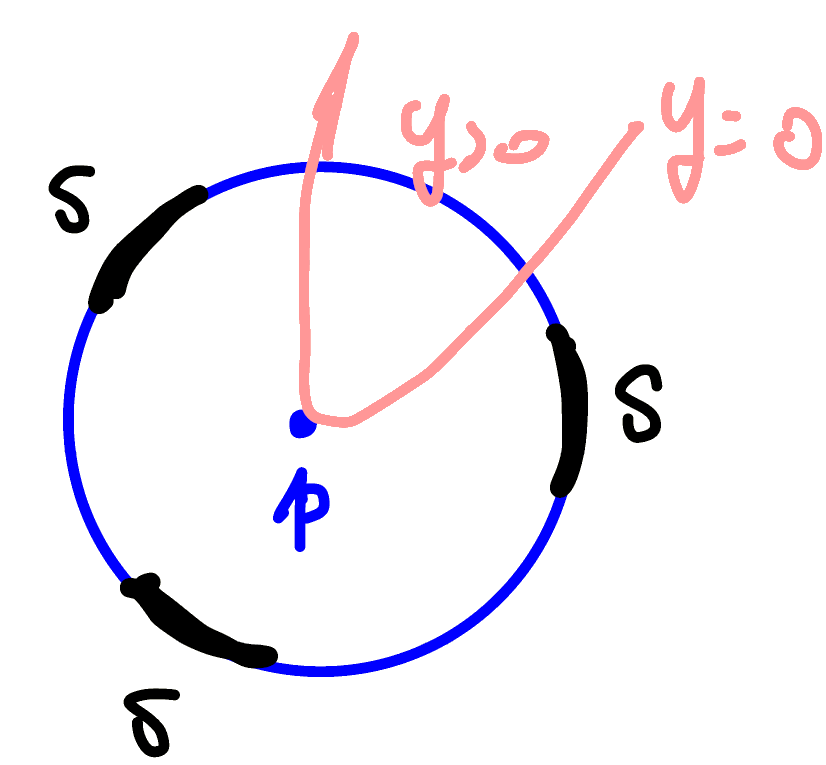
\includegraphics[scale=0.4]{
                    picture/week13/maximum principle.png}
            \end{center}
            By a suitable choice of coordinate \((x,y)\), we can further
            assume \(p\) lies on \(y=0\) and \(S\) lies on \(\{y<0\}\).
            Consider coordinate \(y(q)\) for \(\forall q\in B_p(r)\),
            then \(y\) is a smooth function on \(\bar{B}\).
            
            Note that
            \begin{enumerate}[(1)]
                \item \(y(p)=0\), and \(y<0\) on \(S\).
                \item \(|\nabla y|^2=|g^{22}|\neq 0\)(By
                positive-definiteness).
                \item \(|\Delta y|=|g^{ij}\Gamma\indices*{_{ij}^2}|
                \le A\) for some constant \(A>0\).
            \end{enumerate}
            Let \(h=e^{cy}-1\) for \(c\gg 1\), then
            \begin{enumerate}[(1)]
                \item \(h(p)=0\).
                \item \(\Delta h=c e^{cy}\left(c|\nabla y|^2\right)+
                \Delta y\). Note that \(|\Delta y|\le A\),
                \(|\nabla y|\neq 0\), we
                can choose \(c\) sufficiently large such that
                \[
                    \Delta h>0 \text{ on } \bar{B}.    
                \]
                \item \(h<0\) on \(S\).
            \end{enumerate}
Now consider a perturbation of \(f\)
\[
    f_\epsilon=f+\epsilon h,0<\epsilon\ll 1.
\]
Then
\begin{enumerate}[(1)]
    \item \(f_\epsilon(p)=f(p)+\epsilon h(p)=f(p)\).
    \item \(\Delta f_\epsilon=\Delta f+\epsilon \Delta h>0\) on \(\bar{B}\).
    \item \(f_\epsilon\) must attain maximum inside \(B\). Since
    \(\forall x\in \partial B\), if \(x\) lies in \(S=\{x|f(x)\ge f(p)-1\}\),
    note that \(p\) is a local maximum, and \(S\subset \{y<0\}\), then 
    \[f_\epsilon< f_\epsilon(p) \text{ on }S.\]
    If \(x\in \partial B- S\), \ie\ \(f(x)< f(p)-1\), take \(\epsilon\)
    sufficiently small such that \(|\epsilon h(x)|<1\) on \(\partial B\),
    then one has 
    \[f_\epsilon(x)<f_\epsilon(p) \text{ on }\partial B-S.\]
    This contradicts the strong maximum principle.
\end{enumerate}
\end{proof}
\end{enumerate}
\begin{exercise}[Maximum principle in 1-dimensional calculus]
    Show that
    \begin{enumerate}[(1)]
        \item \(x\in \mathbb{R}\), \(f''(x)>0\), then \(f\) has no upper
        bound.
        \item \(x\in \mathbb{R}\), \(f''(x)\ge 0\), if
        \(\exists x_0\in\mathbb{R}\) such that \(f(x_0)=A=\max f(x)\),
        then \(f(x)=A\) for all \(x\in \mathbb{R}\).
    \end{enumerate}
\end{exercise}
\section{Induced covariant derivative on tensor fields}
Let \(\nabla\) be the Levi0Civita connection on \((M,g)\), then for 
\(\forall\) vector field \(X\in \Gamma(TM)\), the covariant derivative
\(\nabla_X\) is 
\[
    \nabla_X\colon \Gamma(TM)\to \Gamma(TM)    
\]
\[
    Y\mapsto \nabla_X Y    
\]
and locally 
\[
    \nabla_{\pdv{x^i}}\pdv{x^j}=\Gamma\indices*{_{ij}^k}\pdv{x^k}.    
\]
Since \(T^* M\) is the dual bundle of \(TM\), we can extend \(\nabla_X\)
on \(T^*M\) as 
\[
    \nabla_X\colon \Gamma(T^*M)\to \Gamma(T^*M)    
\]
\[
    \omega\mapsto  \nabla_X \omega  
\]
such that \(\forall Y\in \Gamma(TM)\)
\[
    \left(\nabla_X \omega\right)(Y)
    =\nabla_X\left(\omega(Y)\right)-\omega\left(\nabla_X Y\right).
\]
Locally, \(\Gamma(T^*M)=\Span\{dx^1,\ldots,dx^n\}\)
\begin{align*}
    \left(\nabla_{\pdv{x^i}}d x^j\right)\left(\pdv{x^k}\right)
    &=\nabla_{\pdv{x^i}}\left(d x^j \left(\pdv{x^k}\right)\right)-
    d x^j\left(\nabla_{\pdv{x^i}}\pdv{x^k}\right)\\
    &=- dx^j\left(\Gamma\indices*{_{ik}^ p}\pdv{x^p}\right)\\
    &=-\Gamma\indices*{_{ik}^j}.
\end{align*}
\(\Rightarrow \boxed{
    \nabla_{\pdv{x^i}}d x^j =-\Gamma\indices*{_{ik}^j} dx^k
}\).
Now, let \(T\) be a \(p,q\)-tensor
\[
    T=\tensor*{T}{^{i_1\ldots i_p}_{j_1\ldots j_q}}
        \pdv{x^{i_1}}\otimes \ldots \otimes\pdv{x^{i_p}}\otimes 
        dx^{j_1}\otimes\ldots \otimes dx^{j_q}.    
\]
Then
\begin{align*}
    \nabla_k T&=\nabla_k \left(
        \tensor*{T}{^{i_1\ldots i_p}_{j_1\ldots j_q}}
        \pdv{x^{i_1}}\otimes \ldots \otimes\pdv{x^{i_p}}\otimes 
        dx^{j_1}\otimes\ldots \otimes dx^{j_q}
        \right)\\
        &=\partial_k \tensor*{T}{^{i_1\ldots i_p}_{j_1\ldots j_q}}
        \pdv{x^{i_1}}\otimes \ldots \otimes\pdv{x^{i_p}}\otimes 
        dx^{j_1}\otimes\ldots \otimes dx^{j_q}\\
        &\phantom{=}+\sum_{\alpha=1}^p
        \tensor*{T}{^{i_1\ldots i_\alpha\ldots i_p}_{j_1\ldots j_q}}
        \pdv{x^{i_1}}\otimes \ldots \otimes
        \nabla_k\left(\pdv{x^i_{\alpha}}\right)\otimes
        \ldots \otimes\pdv{x^{i_p}}\otimes 
        dx^{j_1}\otimes\ldots \otimes dx^{j_q}\\
        &\phantom{=}+\sum_{\beta=1}^q
        \tensor*{T}{^{i_1\ldots i_p}_{j_1\ldots j_\beta \ldots j_q}}
        \pdv{x^{i_1}}\otimes \ldots \otimes\pdv{x^{i_p}}\otimes 
        dx^{j_1}\otimes\ldots\otimes \nabla_k\left(
        d x^{j_\beta}\right)\otimes\ldots \otimes dx^{j_q}\\
        &=\partial_k \tensor*{T}{^{i_1\ldots i_p}_{j_1\ldots j_q}}
        \pdv{x^{i_1}}\otimes \ldots \otimes\pdv{x^{i_p}}\otimes 
        dx^{j_1}\otimes\ldots \otimes dx^{j_q}\\
        &\phantom{=}+\sum_{\alpha=1}^p
        \tensor*{T}{^{i_1\ldots \gamma\ldots i_p}_{j_1\ldots j_q}}
        \Gamma\indices*{_{k\gamma}^{i_\alpha}}
        \pdv{x^{i_1}}\otimes \ldots\otimes\pdv{x^{i_p}}\otimes 
        dx^{j_1}\otimes\ldots \otimes dx^{j_q}\\
        &\phantom{=}-\sum_{\beta=1}^q 
        \tensor*{T}{^{i_1\ldots i_p}_{j_1\ldots\theta \ldots j_q}}
        \Gamma\indices*{_{kj_\beta}^\theta}
        \pdv{x^{i_1}}\otimes \ldots \otimes\pdv{x^{i_p}}\otimes 
        dx^{j_1}\otimes\ldots \otimes dx^{j_q}.
\end{align*}
\begin{align*}
    \therefore\nabla_k T&=\left(
    \partial_k \tensor*{T}{^{i_1\ldots i_p}_{j_1\ldots j_q}}
    +\sum_{\alpha=1}^p
    \tensor*{T}{^{i_1\ldots \gamma\ldots i_p}_{j_1\ldots j_q}}
    \Gamma\indices*{_{k\gamma}^{i_\alpha}}\right.\\
    &\phantom{aaaaaaaaaaa}\left.
    -\sum_{\beta=1}^q 
        \tensor*{T}{^{i_1\ldots i_p}_{j_1\ldots\theta \ldots j_q}}
        \Gamma\indices*{_{kj_\beta}^\theta}
    \right)\pdv{x^{i_1}}\otimes \ldots \otimes\pdv{x^{i_p}}\otimes 
    dx^{j_1}\otimes\ldots \otimes dx^{j_q},
\end{align*}
or
\[\nabla_k \tensor*{T}{^{i_1\ldots i_p}_{j_1\ldots j_q}}
=\partial_k \tensor*{T}{^{i_1\ldots i_p}_{j_1\ldots j_q}}
+\sum_{\alpha=1}^p
\tensor*{T}{^{i_1\ldots \gamma\ldots i_p}_{j_1\ldots j_q}}
\Gamma\indices*{_{k\gamma}^{i_\alpha}}
-\sum_{\beta=1}^q 
\tensor*{T}{^{i_1\ldots i_p}_{j_1\ldots\theta \ldots j_q}}
\Gamma\indices*{_{kj_\beta}^\theta}\]
\section{Method of Moving Frame}
Let \(\vphi(x^1,x^2)\) be a local coordinate of \(S\hookrightarrow\mathbb{R}^3\).
We have already studied the \emph{equation of motion} of coordinate frame \(\{\vphi_1,
\vphi_2,\vec{N}\}\). Recall that we obtained: 
\begin{equation}\label{eq:recall-eq-motion}
    \begin{cases}
        \vphi_{ij}=\Gamma_{ij}^k\vphi_k+h_{ij}N \\
        N_p=a_p^q\vphi_q
    \end{cases}
.\end{equation}
Where \[
    \begin{cases}
        \Gamma_{ij}^k=\frac{1}{2}g^{kl}(\partial_i g_{jl}+\partial_j g_{il}-\partial_l
        g_{ij}) \\
        a_p^q=-h_{pk}g^{kq}
    \end{cases}
.\] And \(g,h\) be the first and second fundamental forms.

Furthermore, the Gauss-Codazzi equation is the integrability condition to solve
\cref{eq:recall-eq-motion}. This phenomenon can be view more generally as \[
    C^0\xlongrightarrow{\dd}C^1\xlongrightarrow{\dd}C^2
.\] \(\dd^2=0\iff\) integrability condition. 

\subsection{Darboux moving frame (Local orthonormal frame)}
\subsubsection{Curve case}
Let \(\alpha(s)\) be a space curve, \(s\) be the arc-length 
parameter. Recall we have learned the Frenet frame \(\{T,N,B\}\), which is orthonormal
along \(\alpha(s)\) where \[
    T(s)=\alpha'(s),\quad N(s)=\frac{\alpha''(s)}{|\alpha''(s)|},\quad
    B(s)=T(s)\wedge N(s)
.\] And the equation of motion is \[
    \dv{s}\begin{pmatrix}
        T(s) \\ N(s) \\ B(s)
    \end{pmatrix}=\begin{pmatrix}
        0 & k(s) & 0 \\
        -k(s) & 0 & -\tau(s) \\
        0 & \tau(s) & 0
    \end{pmatrix}\begin{pmatrix}
        T(s) \\ N(s) \\ B(s)
    \end{pmatrix}
.\] Recall that we derived the equation from geometry.

Now let \(e_1,e_2,e_3\) be any orthonormal frame along \(\alpha(s)\). Let's fix
\(e_1(s)=\alpha'(s)\) and take differential \[
    \dd{e_i}(s)=e_i'(s)\dd{s}\quad \text{(vector valued 1-form)}
.\] Note \(e_i'(s)\) is still a vector field, let \[
    e_i'(s)=\sum_{j=1}^{3}b_i^j(s)e_i(s)
.\] Then \[
    \dd{e_i}(s)=b_i^j(s)\underbrace{\dd{s}}_{\text{1-form}}
    \underbrace{e_j(s)}_{\text{vector}}
.\] About coefficients \(b_i^j\), since \(\left<e_i,e_j\right> =0\), \(\implies b_i^j
+b_j^i=0\), \ie\ \[
    \begin{cases}
        e_1'=b_1^2e_2+b_1^3e_3 \\
        e_2'=-b_1^2e_1+b_2^3e_3 \\
        e_3'=-b_1^3e_1-b_2^3e_2
    \end{cases}
.\] By fixing \(e_1=\alpha'\), any other orthonormal frame \(\{e_1,\tilde{e}_2,
\tilde{e}_3\}\) is obtained by rotating \(e_2\) and \(e_3\). \ie\ \[
    \begin{pmatrix}
        e_2 \\ e_3
    \end{pmatrix}=\begin{pmatrix}
        \cos\theta & \sin\theta \\
        -\sin\theta & \cos\theta
    \end{pmatrix}\begin{pmatrix}
        e_2 \\ e_3
    \end{pmatrix}
.\] Then we have \[
    (b_1^2,b_1^3)=(\tilde{b}_1^2,\tilde{b}_1^3)\begin{pmatrix}
        \cos\theta & \sin\theta \\
        -\sin\theta & \cos\theta
    \end{pmatrix}
.\] By choosing \(\theta\), we can let \(\tilde{b}_1^3=0\), then \[
    \begin{cases}
        \tilde{e}_1'=\tilde{b}_1^2 \\
        \tilde{e}_2'=-\tilde{b}_1^2\tilde{e}_1+\tilde{b}_2^3\tilde{e}_3 \\
        \tilde{e}_3'=-\tilde{b}_2^3\tilde{e}_2
    \end{cases}
.\] Since \(\alpha''(s)=\tilde{e}_1'(s)=\tilde{b}_1^2\tilde{e}_2=k(s)N(s)\),
we see \(\tilde{b}_1^2=k\) up to a sign. If we further let \(\tilde{e}_2=N\),
then \(\tilde{e}_3=\tilde{e}_1\wedge \tilde{e}_2\) is just \(B\). Hence
\(\tilde{b}_2^3=\tau\).

\subsubsection{Surface case}
Our next goal is to study the 1st and 2nd fundamental form
in terms of local orthonormal frame.

\textbf{Existence:} \\
Let \(\vphi(x^1,x^2)\) be a local coordinate chart on \(U\subset S\), then \(TS\big|_U
=\Span{\vphi_1,\vphi_2}\). Let \[
    e_1=\frac{\vphi_1}{|\vphi_1|},\quad e_2=\frac{\vphi_2-\left<\vphi_2,e_1\right> e_1}
    {|\vphi_2-\left<\vphi_2,e_1\right> e_1|}
.\] Then \(\{e_1,e_2\}\) is an orthonormal frame. Moreover, let \(e_3=e_1\wedge e_2\),
then \(e_3\) is unit normal vector field on \(U\). \(\{e_1,e_2,e_3\}\) gives
an orthonormal frame of \(\mathbb{R}^3\) on \(U\).

For any other orthonormal frame \(\{\tilde{e}_1,\tilde{e}_2\}\) on \(U\), it differs
from \(\{e_1,e_2\}\) by an \(SO(2)\) matrix \[
    R(x^1,x^2)=\begin{pmatrix}
        \Gamma_{11}(x^1,x^2) & \Gamma_{12}(x^1,x^2) \\
        \Gamma_{21}(x^1,x^2) & \Gamma_{22}(x^1,x^2)
    \end{pmatrix}
.\] And for any \(p\in U\), \(\det R(p)=1\).

Now, let's assume \(\{e_1,e_2\}\) be any orthonormal frame on \(U\), \(e_3=e_1\wedge 
e_2\). Then there exists a linear transformation \(T=T(x^1,x^2)\in GL(2)\), such that
\[
    \begin{pmatrix}
        \vphi_1 \\ \vphi_2
    \end{pmatrix}=T\begin{pmatrix}
        e_1 \\ e_2
    \end{pmatrix}\implies \begin{cases}
        \vphi_1=t_1^1e_1+t_1^2e_2 \\
        \vphi_2=t_2^1e_1+t_2^2e_2
    \end{cases}
.\] Note \(\vphi=\vphi(x^1,x^2)\), 
\begin{flalign*}
    \implies\dd{\vphi}&=\vphi_1\dd{x^1}+\vphi_2\dd{x^2} &
    \implies &\dd{\phi} \text{ is a vector valued differential 1-form on }U \\
    &&&\text{\ie\ }\dd{\vphi}\in \Gamma(U,\vphi^*(T\mathbb{R}^3\otimes T^*U))
    \text{(basis change)}&=(t_1^1e_1+t_1^2e_2)\dd{x^1}+(t_2^1e_1+t_2^2e_2)\dd{x^2} \\
    &=(t_1^1\dd{x^1}+t_2^1\dd{x^2})e_1+(t_1^2\dd{x^1}+t_2^2\dd{x^2})e_2 \\
    &=\omega^1e_1+\omega^2e_2
.\end{flalign*}
Where \((\omega^1,\omega^2)=(\dd{x^1},\dd{x^2})\cdot T\). \ie\ in terms of orthonormal
frame \(\{e_1,e_2\}\) on \(U\), \[
    \dd{\vphi}=\omega^1e_1+\omega^2e_2
.\] 

Now, we study the 1st and 2nd fundamental form in terms of \(\{e_1,e_2\}\).
Recall that \[
    I=(\dd{s}^2_{\mathbb{R}^3})\big|_S=\delta_{ij}\dd{y^i}\dd{y^j}
    =(\dd{y^1})^2+(\dd{y^2})^2+(\dd{y^3})^2
.\] Note \(\vphi=\vphi(x^1,x^2)=(y^1(x^1,x^2),y^2(x^1,x^2),y^3(x^1,x^2))\). Then \[
    \dd{\vphi}=(\dd{y^1},\dd{y^2},\dd{y^3})
.\] Hence \[
    I=\left<\dd{\vphi},\dd{\vphi}\right> _{\mathbb{R}^3}
.\] Plug in \(\dd{\vphi}=\omega^1e_1+\omega^2e_2\), we have \[
    I=\left<\omega^1e_1+\omega^2e_2,\omega^1e_1+\omega^2e_2\right>_{\mathbb{R}^3}
    =(\omega^1)^2+(\omega^2)^2
.\]
\begin{remark}\hfill
\begin{itemize}
\item \(\{\omega^1,\omega^2\}\) are dual coframe of \(\{e_1,e_2\}\), \ie\ \(\omega^i
    (e_j)=\delta^i_j\).
\item \(\{\omega^1,\omega^2\}\) is orthonormal frame on \(T^*U\).
\end{itemize}
\end{remark}

Next, we study the 2nd fundamental form in terms of \(\{e_1,e_2\}\) and \(e_3=e_1
\wedge e_2\). \(\dd{e_i}\) is vector valued 1-forms on \(U\), and \(\{e_1,e_2,e_3\}\)
is basis for \(\mathbb{R}^3\), so \[
    \dd{e_i}=\omega_i^je_j
.\] Where \(w_i^j\) are differential 1-forms on \(U\). Moreover \[
    \omega_i^j=\left<\dd{e_i},e_j\right> =-\left<e_i,\dd{e_j}\right> =-\omega_j^i
.\] Since \(e_3\) is the unit normal, \(-\dd{e_3}\) is just the Weingarten map, hence
\begin{align*}
    \II&=-\left<\dd{e_3},\dd{\vphi}\right> =-\left<\omega_3^1e_1+\omega_3^2e_2,
    \omega^1e_1+\omega^2e_2\right> \\
    =-\omega_3^1\omega^1-\omega_3^2\omega^3=\omega_1^3\omega^1+\omega_2^3\omega^2
.\end{align*}

In summary, if \(\{e_1,e_2,e_3\}\) is orthonormal frame of \(S\) on \(U\), with
\(e_1,e_2\in T_U S\), \(e_3\in N_U S\), and \(\omega^1,\omega^2\in T_U^*S\) is
dual coframe of \(\{e_1,e_2\}\), then \[
    \begin{cases}
        \dd{e_i}=\omega_i^je_j \\
        \omega_i^j+\omega_j^i=0
    \end{cases},\quad \begin{cases}
        I=(\omega^1)^2+(\omega^2)^2 \\
        \II=\omega_1^3\omega^1+\omega_2^3\omega^2
    \end{cases}
.\] 
\begin{remark}\hfill
\begin{itemize}
\item Here \(\omega^i,\omega_j^k\) are covariant 1-tensors, \[
    \omega^i\omega_i^k=\frac{1}{2}(\omega^i\otimes\omega_i^k+\omega_i^k\otimes\omega^i)
    \quad \text{(symmetrization of }\omega^i,\omega_j^k\text{)}
.\] 
\item Since \(\omega_1^3,\omega_2^3\) are differential 1-forms on \(U\), \ie\ \(
    \omega_1^3,\omega^3\in T_U^*S=\Span\{\omega^1,\omega^2\}\), we can let \[
        \begin{cases}
            \omega_1^3=A_{11}\omega^1+A_{12}\omega^2 \\
            \omega_2^3=A_{21}\omega^1+A_{22}\omega^2
        \end{cases}
    .\] Then \[
        \II=(\omega^2,\omega^2)\begin{pmatrix}
            A_{11} & A_{12} \\
            A_{21} & A_{22}
        \end{pmatrix}\begin{pmatrix}
            \omega^1 \\ \omega^2
        \end{pmatrix}
    .\] In particular, since \(\II\) is symmetric, \(A_{12}=A_{21}\).
\end{itemize}

\subsection{Exterior Derivative \& Cartan's Structure Equation}
\subsubsection{Differential forms}
Reference: Kodaira's book \emph{Complex manifolds and Deformation of Complex Structures}

Let \(M\) be a smooth manifold of dimension \(n\), let \(\{U_\alpha\}\) be a coordinate covering of \(M\).




\end{remark}

\section{The Hilbert's theorem}
\begin{theorem}[Hilbert's theorem]
    Let \(S\) be a complete and simply connected regular surface with
    Gaussian curvature \(K=-1\), then there is no isometric embedding of
    \(S\) into \(\mathbb{R}^3\).
\end{theorem}
\begin{proof}[Sketch of proof]
    \begin{enumerate}[(1)]
        \item \((S,g)\) is isometric to the hyperbolic plane in 
        \(\mathbb{H}^2\)\\
        \(\Rightarrow\) \(Area(S)=Area(\mathbb{H}^2)=+\infty\).
        \item If \(\exists\) an isometric embedding \(
            \varphi\colon S\to \mathbb{R}^3\), then we can construct a 
            global parametrization of \(S\) with coordinate curves being
            asymptotic lines, and the parametrization forms a
            ``chebyshev net'' such that any quadrilateral of coordinate
            curves has area \(<2\pi\). This implies 
            \[Area(S)<2\pi.\]
    \end{enumerate}
    Then (1) and (2) yields a contradiction.
\end{proof}
\begin{definition}
    A local parametrization \(\phi (u,v)\colon U\subset \mathbb{R}^2\to
    S\) is called a ``chebyshev net'' if the length of opposite sides of
    any quadrilateral formed by coordinate curves are equal.
\end{definition}
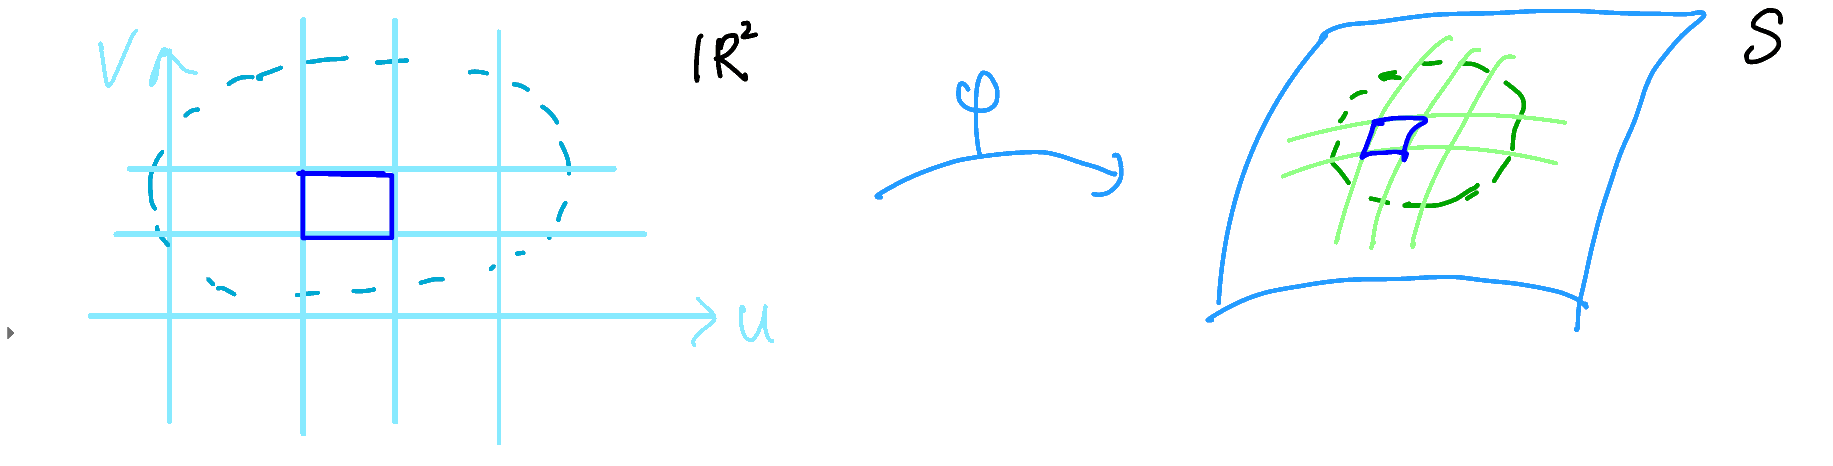
\includegraphics[scale=0.4]{picture/week15/chebyshev net.png}
\begin{proof}[proof of (1)]
    First, from the minding's theorem, we know \(S\) and \(\mathbb{H}\)
    are locally isometric to each other. Let \(p\in S\), \(p'
    \in \mathbb{H}\), the local isometry yields a linear isometry
    \(l\colon T_p S\to T_{p'} \mathbb{H}\).

    To construct a global isometry, let's consider
    \begin{center}
        \begin{tikzcd}
            T_p S \arrow[d, "\exp_p"] \arrow[r, "l"] & T_{p'}\mathbb{H} \arrow[d, "\exp_{p'}"] \\
            S \arrow[r, dashed]                      & \mathbb{H}                             
        \end{tikzcd}
    \end{center}
    By the Hadamard theorem \(\rightarrow\) \(\exp_p\) and \(\exp_{p'}\)
    are diffeomorphism.
    \footnote{
        Hadamard's theorem: let \((M,g)\) be a complete Riemannian manifold
        with \(K_M\le 0\), where \(K_M\) is the sectional curvature, then
        \(\exp_p\colon T_p M\to M\) is a covering map. Moreover, if \(M\)
        is simply connected, then \(\exp_p\) is a diffeomorphism.
    }
    Hence \(f=\exp_p\circ l\circ \exp_{p'}^{-1}\colon S\to \mathbb{H}\)
    is a diffeomorphism. We can further conclude that \(f\) is a local 
    isometry. This follows from the Cartan's theorem:
    \begin{itemize}
        \item Let \((M,g)\), \((M',g')\) be two Riemannian manifolds, 
        \(p\in M\), \(p'\in M'\).
        \item Let \(l\colon T_p M\to T_{p'}M'\) be a linear isometry
        \item \(U\) is a normal neighborhood of \(p\) on which \(\exp_p\)
        is a diffeomorphism.
        \item \(\forall V\in T_q M\), and let \(P_t\) be the parallel transport
        along \(\gamma(t)\), then \(P_t^{-1}(V)\) is a vector in \(T_p M\).
        The linear isometry yields \(l\circ P_t^{-1}(V)\) to be a vector
        in \(T_{p'}M'\). Let \(q'=\exp_{p'}\circ l\circ\exp_{p}^{-1}q
        \in M'\), \(\gamma'(t)\) is the geodesic from \(p'\) to \(q'\)
        and \(P_t'\) is the parallel transport along \(\gamma'(t)\).
        Then using \(P_t '\), we get a vector \(P_t'\circ l\circ 
        P_t^{-1}(V)\\in T_{q'}M'\)
        \(\Rightarrow L_t=P_t'\circ l\circ P_t^{-1}\colon T_q M\to
        T_{q'}M'\) is a linear isometry. If \(\forall\) vectors 
        \(X, Y,Z,W\in T_q M\) we have
        \[
            R(X,Y,Z,W)=R'(L_t(X),L_t(Y),L_t(Z),L_t(W))    
        \]
        then \(f=\exp_{p'}\circ l\circ \exp_p^{-1}\) is a local isometry.
        \begin{center}
            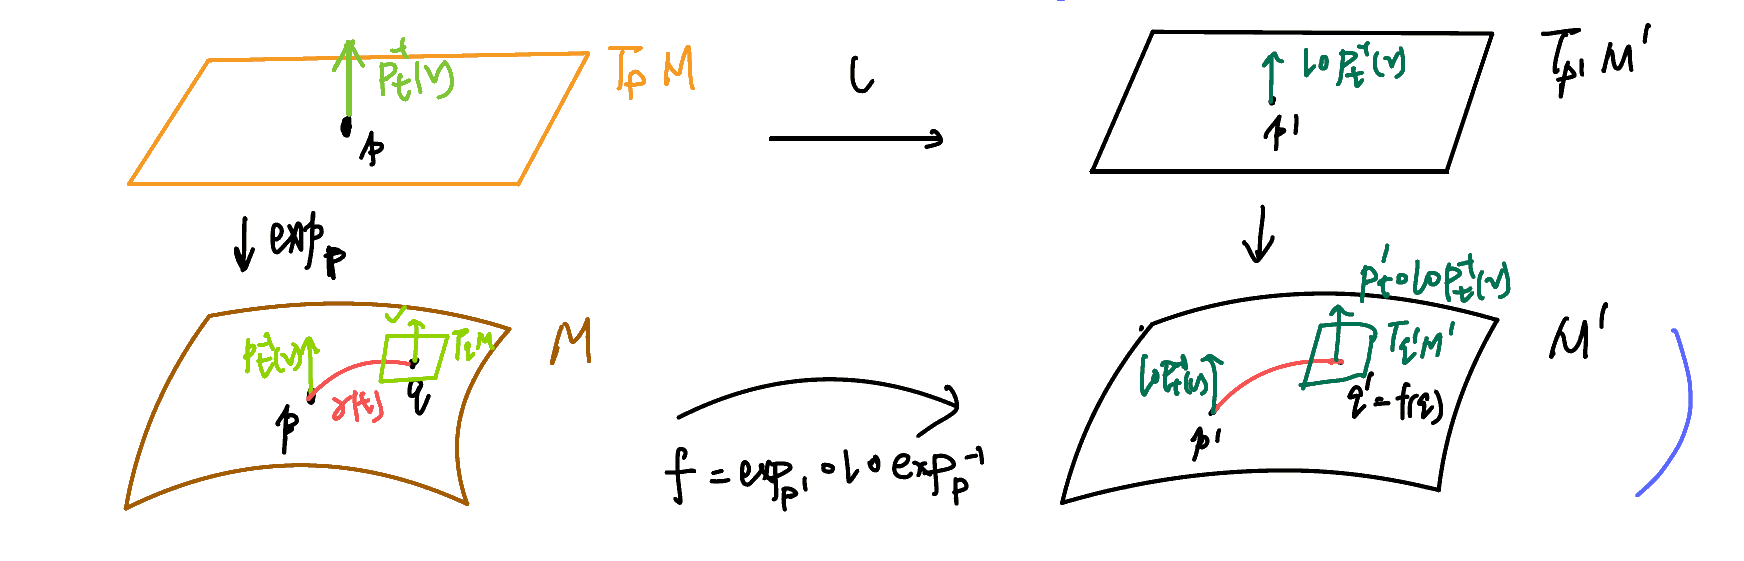
\includegraphics[scale=0.4]{picture/week15/cartan theorem.png}
        \end{center}
    \end{itemize}
    Hence, we see \((S,g)\) and \(\mathbb{H}\) are isometric to each other on
    \(\mathbb{H}^2\). We consider geodesic polar coordinate such that
    \[ds^2=dr^2+\left(\sinh r\right)^2 d\theta^2.\]
    Then the radial geodesic \(\gamma(t)=\exp_p(t\pdv{r})\) defines for all
    time \(t\), \(\Rightarrow t\in (0,+\infty)\)
    \[Area(S)=Area(\mathbb{H})=\int_{0}^{2\pi} \int_{0}^{+\infty}
    \sinh r drd\theta=+\infty\]
\end{proof}
\begin{proof}[proof of (2)]
    Now we assume \(S\) is isometrically embedded into \(\mathbb{R}^3\).

    \underline{Claim 1}: \(\forall p\in S\), \(\exists\) local parametrization
    \((s,t)\) of \(S\), such that the \engordnumber{1} and 
    \engordnumber{2} fundamental form are given by
    \[
      I=ds^2+2\cos \alpha ds dt +dt^2  
    \]   
    \[\II=2\sin\alpha ds dt\]
    where \(\alpha=\alpha(s,t)\) satisfies the Sine-Gordan equation
    \[\alpha_{st}=\sin \alpha,\quad 0<\alpha<\pi\]
    From this expression of I and II, we see
    \begin{enumerate}[(1)]
        \item the length of opposite sides of coordinate quadrilateral
        are the same \(\Rightarrow\) \((s,t)\) forms a chebyshev net,
        \(\alpha\) is the angle between \(s\)-curve and \(t\)-curve.
        \begin{center}
            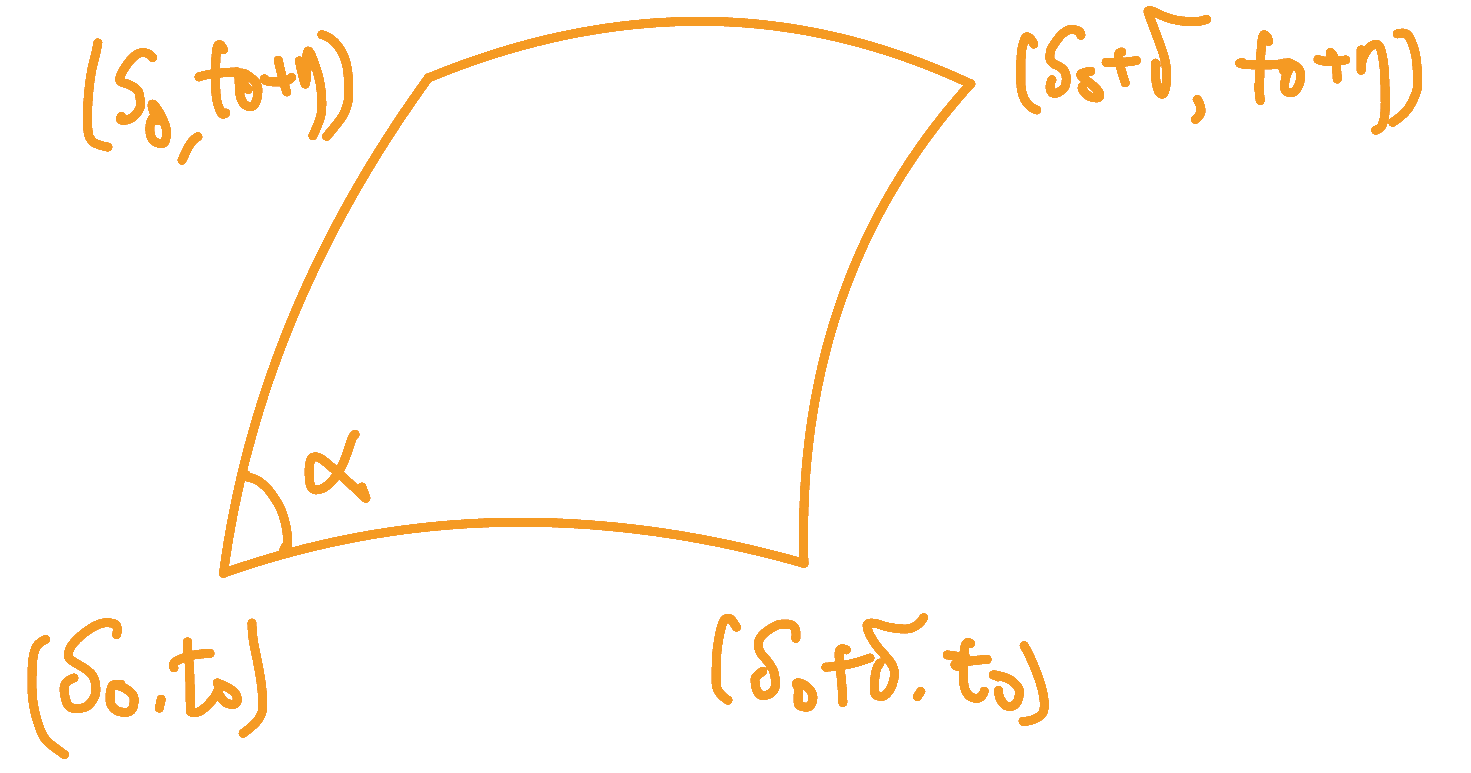
\includegraphics[scale=0.2]{picture/week15/quadrilateral.png}
        \end{center}
        \item coordinate \(s\)-curve and \(t\)-curve are asymptotic lines
    \end{enumerate}
    \begin{proof}[Proof of claim 1]
        \(K=-1\) on \(S\) \(\Rightarrow\) all pairs are umbilical.
        Hence, we can first choose local parametrization \(x^1,x^2\)
        such that 
        \[I=g_{11}(dx^1)^2+g_{22}(dx^2)^2\]
        \[II=h_{11}(dx^1)^2+h_{22}(dx^2)^2\]
    \(\Rightarrow\) principal curvatures \(k_1=\frac{h_{11}}{g_{11}},
    k_2=\frac{h_{22}}{g_{22}}\).
    The codazzi equation is 
    \[\frac{\partial_2k_1}{k_2-k_1}=\partial_2 \log \sqrt{g_{11}}\]
    \[\frac{\partial_1k_2}{k_1-k_2}=\partial_1 \log \sqrt{g_{22}}\]
    Since \(k_1k_2=-1\), we set 
    \[
        k_1=\tan\theta,\quad k_2=-\cot\theta,\quad 0<\theta<\frac{\pi}{2}    
    \]
    \(\Rightarrow k_1-k_2=\tan\theta+\cot \theta=
    \frac{1}{\sin\theta\cos\theta}\).
    Then the codazzi equation 
    \end{proof}
\end{proof}

%==============================%

% \printbibliography{}
\end{document}
